\documentclass[11pt,a4paper,english,twocolumn]{article}
\usepackage{unir_paper}
\usepackage{subcaption}
\usepackage{tablefootnote}

%---------------------------
%título del trabajo y autor
%---------------------------
\title{Machine Learning Tools for Open Cluster Characterization with Gaia DR2 Data}
\author{CD. Álvaro, C. Guzman, J. Álvaro}
\date{24th of January, 2021}


%---------------------------
%marges
%---------------------------
%\usepackage[margin=1.9cm]{geometry}
%---------------------------
%---------------------------
%---------------------------
%---------------------------

\resumen{
The characterization and understanding of \emph{Open Clusters} (OCs) allow us to
understand better properties and mechanisms about the Universe such as stellar
formation and the regions where these events occur. They also provide information
about stellar processes and the evolution of the galactic disk.

In this paper, we present a novel method to characterize OCs. Our method employs a
model built on \emph{Artificial Neural Networks} (ANNs). More specifically, we adapted
a state of the art model, the \emph{Deep Embedded Clustering} (DEC) model for our purpose.
The developed method aims to improve classical state of the arts techniques. We improved
not only in terms of computational efficiency (with lower computational requirements),
but in usability (reducing the number of hyperparameters to get a good characterization
of the analyzed clusters). For our experiments, we used the \emph{Gaia DR2 database} as
the data source, and compared our model with the clustering technique \emph{K-Means}. Our
method achieves good results, becoming even better (in some of the cases) than current techniques.
}

\palabrasclave{
    characterization,
    data analysis,
    deep embedded clustering,
    gaia,
    machine learning,
    open cluster
}

\begin{document}
\twocolumn[
\begin{@twocolumnfalse}
\maketitle
\end{@twocolumnfalse}
]

%\renewcommand{\listfigurename}{Índice de Ilustraciones}
%\renewcommand{\listtablename}{Índice de Tablas}
%\renewcommand{\contentsname}{Índice de Contenidos}
%\renewcommand{\figurename}{Figura}
%\renewcommand{\tablename}{Tabla}
%\twocolumn


%\frontmatter
%\tableofcontents
%\listoffigures
%\listoftables

\section{Introduction}

Stellar OCs~\cite{janes1982open} are groups of stars gravitationally
bounded originated from a single molecular gas cloud.
They share the same chemical composition and age, and that is the reason
that their metallicity must be uniform since those stars were born from
the same gas cloud and at the same time stage. Likewise, they have similar
relative positions inherited from their original gas cloud, which means that
their distances to the Earth are the same. Therefore, they have a narrow
dispersion in their parallax value. Moreover, they share similar values
of proper motion, both in right ascension and declination. For all these
properties, we can see why the stellar OCs are relevant to understand the
spiral structure, dynamics, and chemical evolution of our galaxy.

The study of OCs advanced thanks to the huge and precise dataset
from the Gaia DR2 mission, available since 2018 from~\cite{collaboration2016description}
and~\cite{gaia2018gaia}. Although, the Gaia DR2 database misreported the chemical
composition of some OCs, the database has helped to review already known OCs and
to find new ones.

The characterization of an OC refers to the statistical determination
of the stars that form it. Therefore, the characterization is based on
the probability of a star to be a member of the cluster~\cite{sampedro2016caracterizacion}.

Normally, the characterization process considers astrometric features such as
proper motion in right ascension and declination, or parallax.
In some cases~\cite{oliveira2013fitting}, it also considers photometric features,
which helps to generate the H-R diagram~\cite{hypki2018gaia} of the OC candidate stars.
Those OC candidates should present a sharp profile corresponding to an isochrone curve
derived from a theoretical model. The model considers metallicity, mass and brightness
of the stars involved. For all this purpose, we used a set of tools that require
supervised and parameterized models. It means that we need a previous knowledge of the
cluster, otherwise we must repeat the process iteratively to achieve valid results.

In the present paper, we propose a machine learning model capable of characterizing
OCs inside a stellar region with no previous knowledge about the region.
Our model takes advantage of some features (such as proper motion in right ascension
and declination, and parallax) to train an Artificial Neural Network.
The ANN clusters all the stars within a given region in groups.
One of those groups will be the open cluster that interests us.

Our model contributes with several novelties: i) it is \emph{non-supervised} and
\emph{non-parameterized}, making easier the automation process of analyzing a
wide range of regions with different typologies, and ii) it is computationally
efficient to run in common workstations because it has been developed with
Python using the Keras framework which takes advantage of modern GPUs to perform
its computations. That increases significantly the computational capacity of
our model doing it possible to run on regular workstations.

This paper is organized as follows. Section~\ref{sec:related_works} presents
some related works and Section~\ref{sec:aims_and_method} describes in detail
our model. The following Section~\ref{sec:results}, shows the results and compares
them with a method that involves tools from the Virtual Observatory (VO) such as
Clusterix~\cite{balaguer2020clusterix}. Finally, the last section concludes and
outlines future research lines.

\section{Related work}
\label{sec:related_works}

In~\cite{castro2020hunting}, they present one of the initial approaches to detect OCs.
They search for overdensities in the astrometric space of the galactic disk. Then,
they identify with photometric information possible OCs. Although it seems easy,
it is quite hard to face the problem that the near field around the OC has two kinds of
populations. The first population belongs to the members of the OC stars (from tens or
hundreds to a few thousand). The second population has a background of stars that do
not belong to the OC (from tens to hundreds of thousands). Thus, we summarize our problem
in finding out which stars belong to the OC.

Other works (TOPCAT~\cite{taylor2005topcat}, Clusterix 2.0~\cite{balaguer2020clusterix},
Aladin~\cite{bonnarel2000aladin}, or VOSA~\cite{bayo2008vosa}), first analyze the proper
motion configuration space of the region of interest. TOPCAT cannot find an open cluster.
Instead, it requires parameterizing some of the properties of the cluster. This last
process requires previous knowledge of the cluster. In other words, they perform a supervised
and manual selection of groups based on overdensities in the proper motion configuration space.
Clusterix 2.0 is an interactive web-based tool that can help the choice of groups. Take the
proper motion diagram without making any previous assumptions about the membership of the
candidate star. And empirically determine the frequency functions. It employs normal Gaussian
kernel functions, defined as:

\begin{equation*}
  K(a, b) = \frac{1}{2 \pi h^{2}} \exp{ \left[ - \frac{1}{2}\frac{\left( a - a_{i} \right)^{2} + \left( b - b_{j} \right)^{2}}{ h^{2}} \right]}
\end{equation*}

where \(( a, b )\) are the proper motion configuration space, \(( i, j )\) is a point
located in the center of that provides the maximum contribution for calculating the
local density, and \(h\) is the \emph{smoothing} parameter, which it is measured in the
same units as the proper motion.

Clusterix critically depends on the selection of three radii in the studied region.
The inner radius contains stars belonging or not to the cluster. While the outermost
radii defines a ring which only contains stars that do not belong to the cluster.
In addition, it is also sensitive to other parameters, such as the soften parameter
\emph{h}, or other restrictions related with the searched proper motions.

If the analysis performed by Clusterix is successful, it returns the probability of
each star to belong to the open cluster. The results can be imported then into TOPCAT
to continue the refining process to get a valid characterization.

Another recent approach~\cite{castro2020hunting} solves the problem using machine
learning techniques. It searches systematically for overdensities in the astrometric
space of the galactic disk and a subsequent identification of open clusters using
photometric information. It includes two phases:

\begin{enumerate}
  \item it employs DBSCAN, an unsupervised clustering algorithm, to search for
        overdensities,
  \item and it applies a deep learning ANN to identify isochrone patterns within
        the detected overdensities and thus proceed to confirm them as OCs. They
        trained previously the ANN with magnitude diagrams.
\end{enumerate}

They execute their experiments in the Barcelona Supercomputing Center, MareNostrum 42.
Thereby, the neural network handles the image recognition process with isochrone
patterns without applying theoretical models derived from values such as metallicity
or masses, among other. Their work concludes with the identification of 582 new open
clusters distributed along the galactic disk for a galactic declination bellow 20
degrees, increasing the number of known open clusters by 45\%.

In contrast to~\cite{castro2020hunting}, we lack of a super computer like MareNostrum
for our experiments. For this reason, our aim is to obtain a new novel method that
allows the characterization of open clusters without doing a blind search for clusters
characterization. We advocate of the idea of building an unsupervised and
non-parameterized method. So, it can be suitable for automated processes.

\section{Open Cluster Characterization method}
\label{sec:aims_and_method}

In the literature, we have several clustering algorithms, such as K-Means, Mean-Shift
Clustering, DBSCAN~\cite{ester1996density} among other, that can help us to achieve
our aim. Each one behaves better according to the distribution of the objects to
clusterize. However, we need to set a large number of clusters to find the open cluster
we are looking for. It complicates the identification of the OC because most of the
time falls in many outliers.

The unsupervised \emph{Deep Embedding for Clustering Analysis} (\emph{DEC})
model~\cite{xie2016unsupervised} is a refinement K-Means based on ANN. It starts with
K-Means. And then, it trains an autoencoder to reduce the feature space and pass them
through a Clustering Layer which refines the previous selection.

With all this in mind, our method is based on DEC model. We adapted it to manage data
groups based on the dynamic properties of the stars. Thus, we have an unsupervised
clustering model for open cluster characterization. The model fits a wide range of
clusters without the need for fine-tuning a high number of hyperparameters.

\subsection{Selection of the catalogue}

In this work we make use of Gaia DR2 since DR3 has not been released in time for us to
include it. Gaia DR2 is a multidimensional dataset obtained by ESA's Gaia mission
(located at L2, 1.5 million kilometers from Earth) and operational since 2014. The
catalogue has high precision and accuracy astrometric data for more than 1.7 billion
stellar sources, and magnitudes in three photometric filters (G, BP and RP) for more
than 1,300 million sources.

We start by selecting a region from the OpenClust~\cite{dias2002new} catalogue and
we downloaded it from Gaia DR2 database. The radius of the downloaded region from Gaia
is 1.5 times larger than the one registered in OpenClust, ensuring to include several
stars that do not belong to the open cluster.

\subsection{Selection of features}
\label{sec:feature_selection}

For the selection of features, we studied the Melotte 22 dataset.
Table~\ref{tab:sample_features_melotte22_region} describes an example of the region Melotte 22.
Each row represents the features of a star.

\begin{table}[!htbp]
  \begin{center}
    \resizebox{\columnwidth}{!}{
      \begin{tabular}{c|c|c}
        % \textbf{source\_id} &
        \emph{pmra \((mas \cdot yr^{-1})\)} & \emph{pmdec \((mas \cdot yr^{-1})\)} & \emph{parallax \((mas)\)} \\
        \hline
        % 64035217900973056 &
        2.848682 & -3.291204 & 0.399680 \\
        % 64035217900973440 &
        0.894901 & -3.445501 & 0.416639 \\
        % 64035217901215616 &
        7.924372 & -0.241281 & 0.397743 \\
        % 64035351043566208 &
        -4.433802 & -2.584965 & 0.410695 \\
        % 64035385403304960 &
        0.055990 & -1.760018 & 0.413813 \\
      \end{tabular}
    }
    \caption{Features of Melotte 22 region.}
    \label{tab:sample_features_melotte22_region}
  \end{center}
\end{table}

Proper motion in right ascension (column pmra) and declination (column pmdec) seems
like a natural choice since stars belonging to the same OC share a common motion vector.
Parallax (column parallax) is another relevant feature. It lets us know how far stars
are from us. Besides, since all stars within an open cluster were born from the same
dust cloud, they must all have similar parallax.

However, we are not going to use these raw features. Instead, we are taking a combination
of them. Figure~\ref{fig:features_melotte_22} shows a pairwise relationship of our
combination of features from Melotte 22.

\begin{figure*}[!hbt]
  \centering
  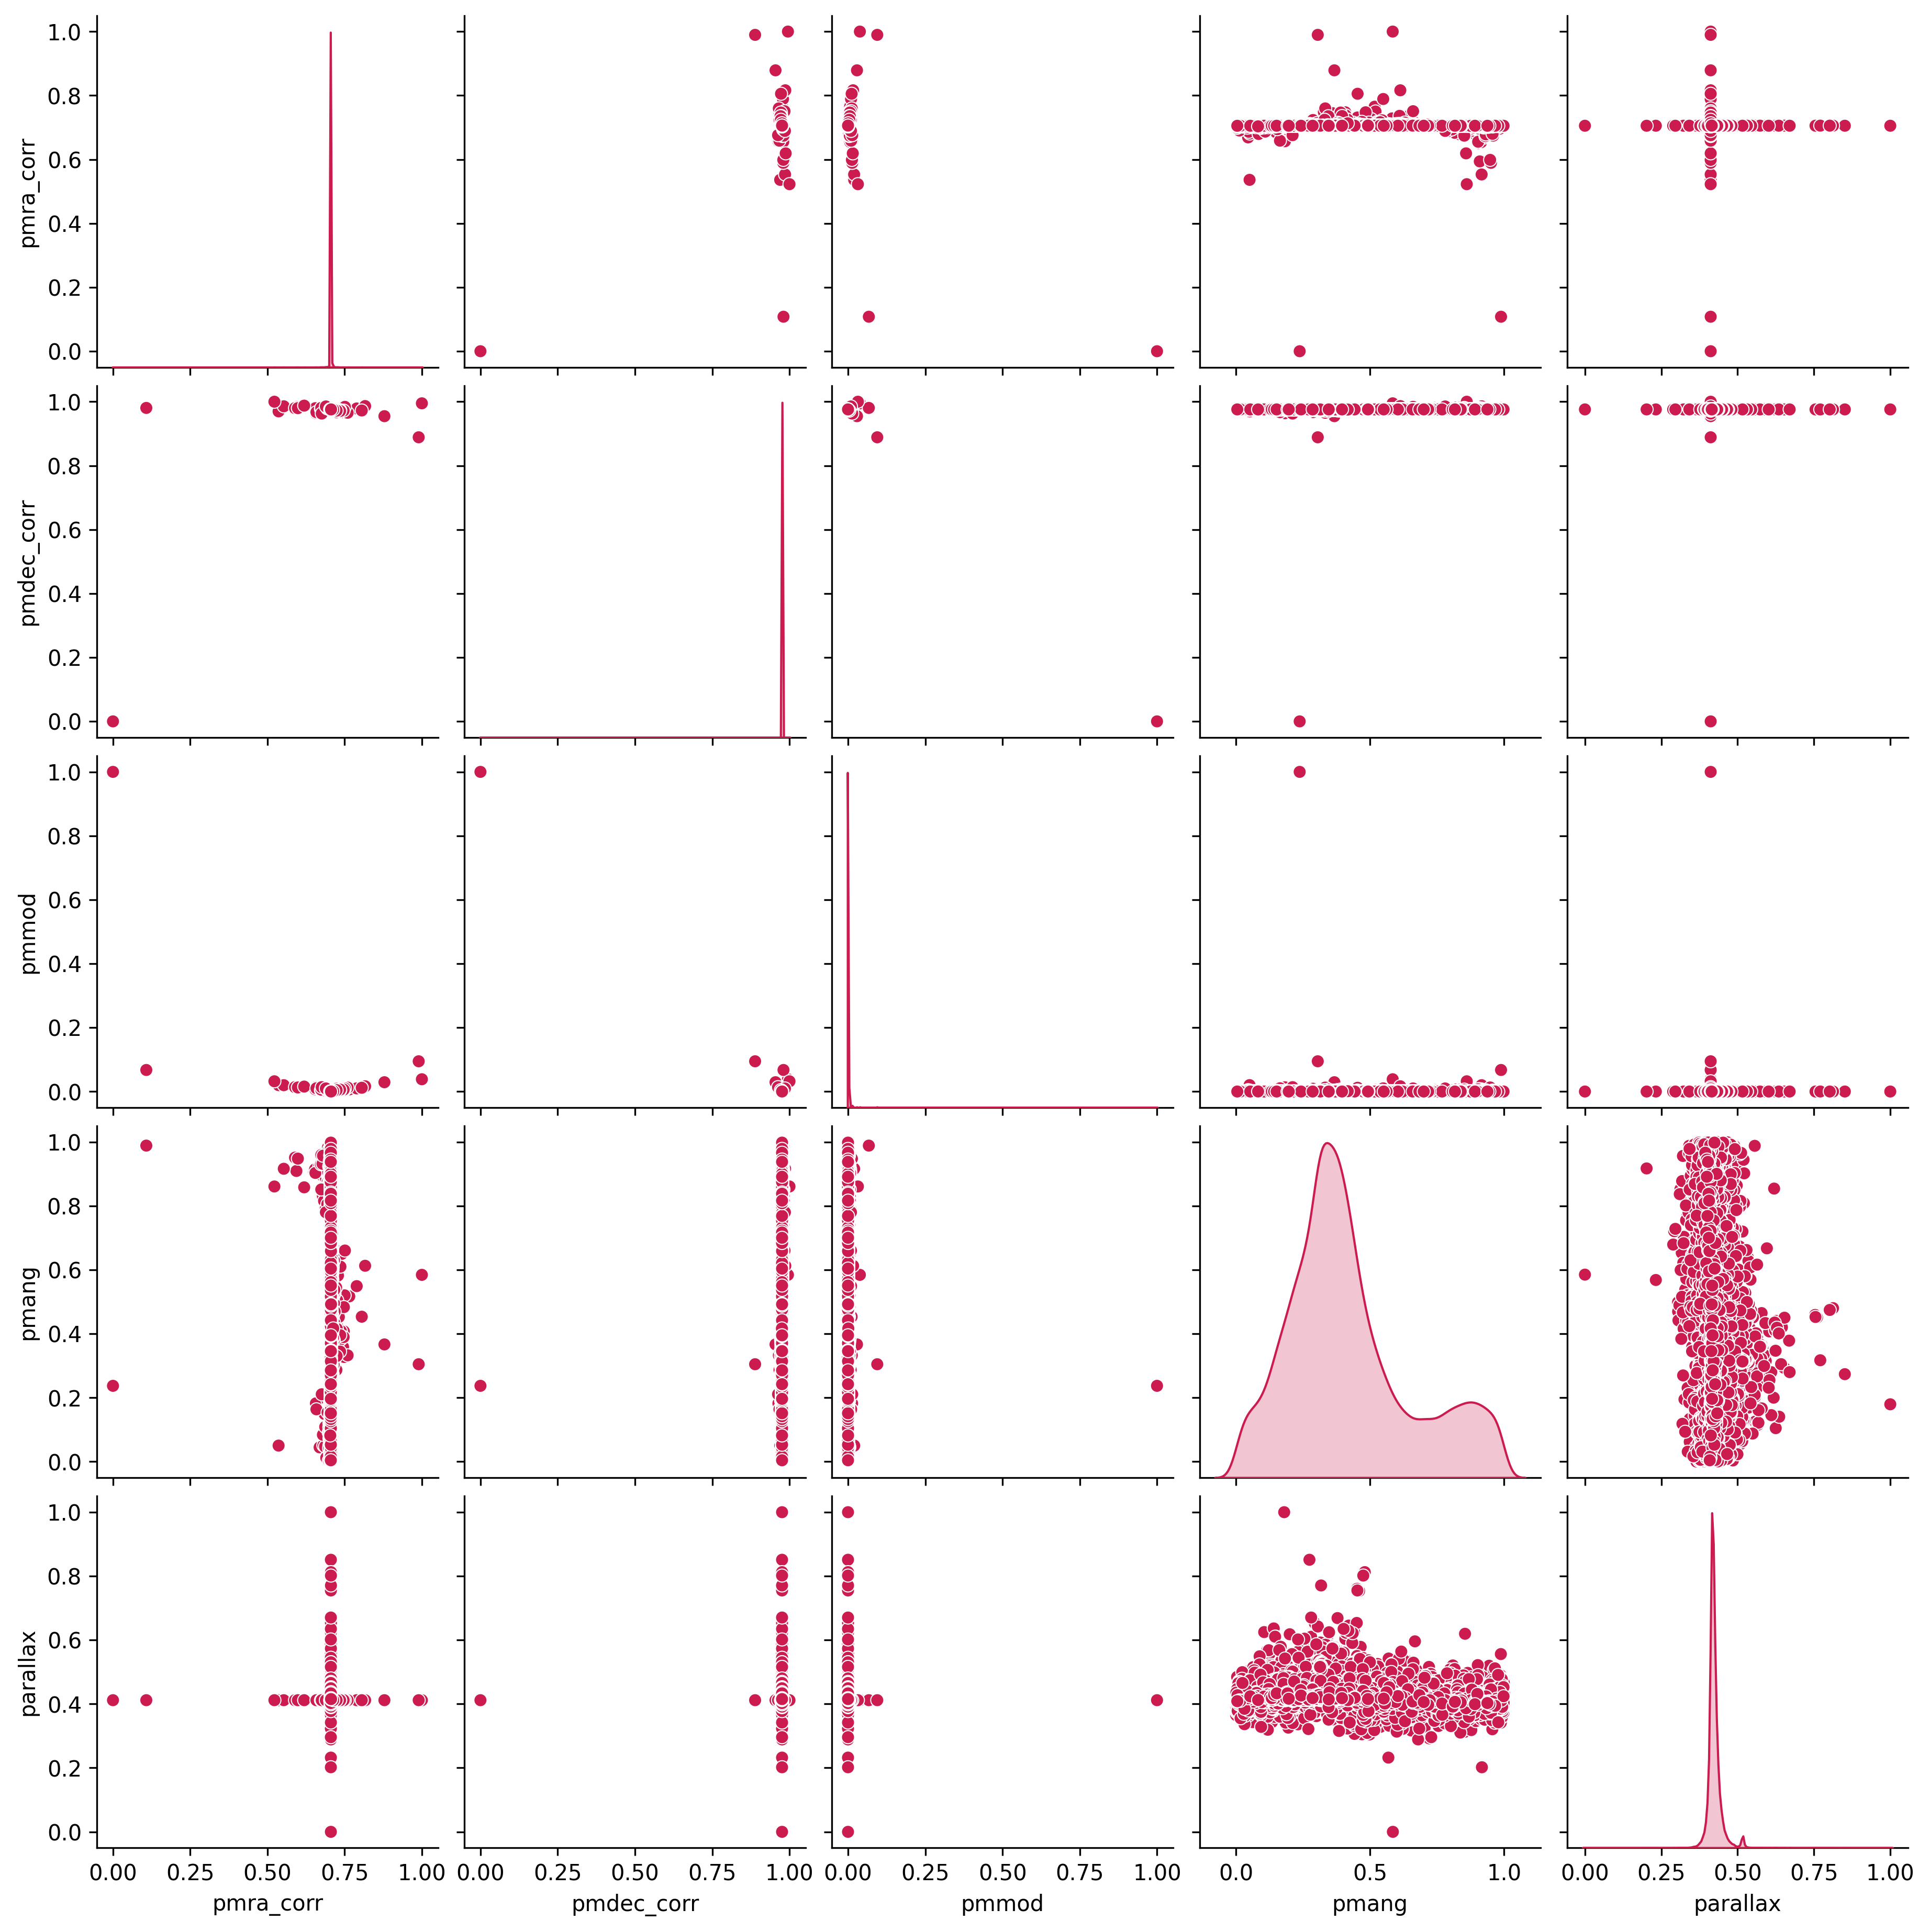
\includegraphics[scale=0.5]{../figures/melotte_22/features_melotte_22.png}
  \caption{Pairwise relationships among variables using Melotte 22 data}
  \label{fig:features_melotte_22}
\end{figure*}

First, we correct proper motion in right ascension and declination by dividing them by
the parallax (variables pmra\_corr and pmdec\_corr, respectively). That way, we normalize
these quantities and help our clustering models to improve their performance. The modulus
of the proper motion (variable pmmod in Figure~\ref{fig:features_melotte_22}) is another
computed property that we considered. We use it to relate both features and therefore
force our model to keep them tight.

\subsection{Deep Open Clustering of stars}
\label{sec:deep_open_clustering}

In this section we explain in more detail our model.

In order to define our model, one of the main problems is that we do not have a labeled
dataset to train a supervised model. Thus, we have to deal with an unsupervised self-trained
model. We adapted the Unsupervised \emph{DEC} model~\cite{xie2016unsupervised} to our requirements.

Same as the DEC model, we have two main components:

\begin{itemize}
  \item \textbf{deep autoencoder:} It is trained before passing the data through the
        \emph{clustering layer}. It is composed by encoder layers followed by decoder
        layers. Recent research has shown that this autoencoder provides meaningful and
        well-separated representations on real-world datasets~\cite{vincent2010stacked}
        and~\cite{hinton2006reducing} to the DEC model.
  \item \textbf{clustering layer:} This layer recibes data transformed by the autoencoder
        and it is iteratively trained until a convergence criterion is met.
\end{itemize}

The deep autoencoder is used to transform the input data into a latent space using a
non-linear mapping function \(f_{\theta} : X \rightarrow Z\).

As it was described in Section~\ref{sec:feature_selection}, the number of features we
deal is not too large. This latent space helps us to start in a reduced number of
features and avoids the \emph{``curse of dimensionality``}~\cite{bellman1961curse}.

The autoencoder is pretrained before fitting the model to generate predictions. Then,
the encoder layers of the autoencoder are used with the aim of transforming input data to
the latent space \(Z\). Once the data has been transformed, a K-Means clusterer is used in
order to make an initial clustering. K-Means cluster centers are used as the initial
weights for the clustering layer.

With that initial configuration, the model iterates alternating between computing an auxiliary
target distribution (Soft Assignment) and minimizing the Kullback-Leiber (KL)
divergence~\cite{kullback1951information} to it.
This unsupervised algorithm allows us to improve the clustering.

\begin{equation}
  p_{ij} = \frac{q^{2}_{ij} / f_{j}}{\sum_{j'}q^{2}_{ij'}/f_{j'}}
  \label{eq:student_tdistribution}
\end{equation}

In the soft assignment stage,
the \emph{Student's t-distribution} is used as a kernel to measure the similarity
between the embedded points and the cluster centroid.
While in the KL divergence minimization the algorithm iteratively refines clusters by learning
from their high confidence assignments with the help of an auxiliary target distribution.
The model is trained by matching the soft assignment to the target distribution.
The choice of this target distribution is crucial for DEC's performance.
In this work we have taken the target distribution from DEC's original paper~\cite{xie2016unsupervised},
which is defined in Equation~\ref{eq:student_tdistribution}.

\begin{figure*}[!hbt]
  \centering
  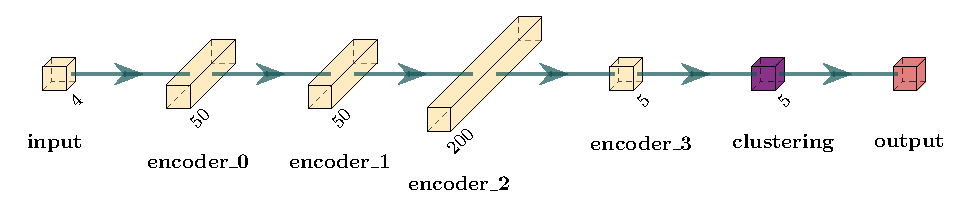
\includegraphics[scale=0.8]{../figures/dec_diagram.pdf}
  \caption{DEC model layer setup}
  \label{fig:dec_model_setup}
\end{figure*}

Figure~\ref{fig:dec_model_setup} shows the layer setup of our DEC model.
It is simpler than the one tested on the original paper~\cite{xie2016unsupervised},
since the number of selected features in our work is smaller than in the original one.
Therefore, using the same configuration would result in a model so
powerful that would incur in overfitting issues unable to make right predictions.

\begin{figure*}[!htbp]
  \centering
  \begin{subfigure}[b]{0.3\textwidth}
    \centering
      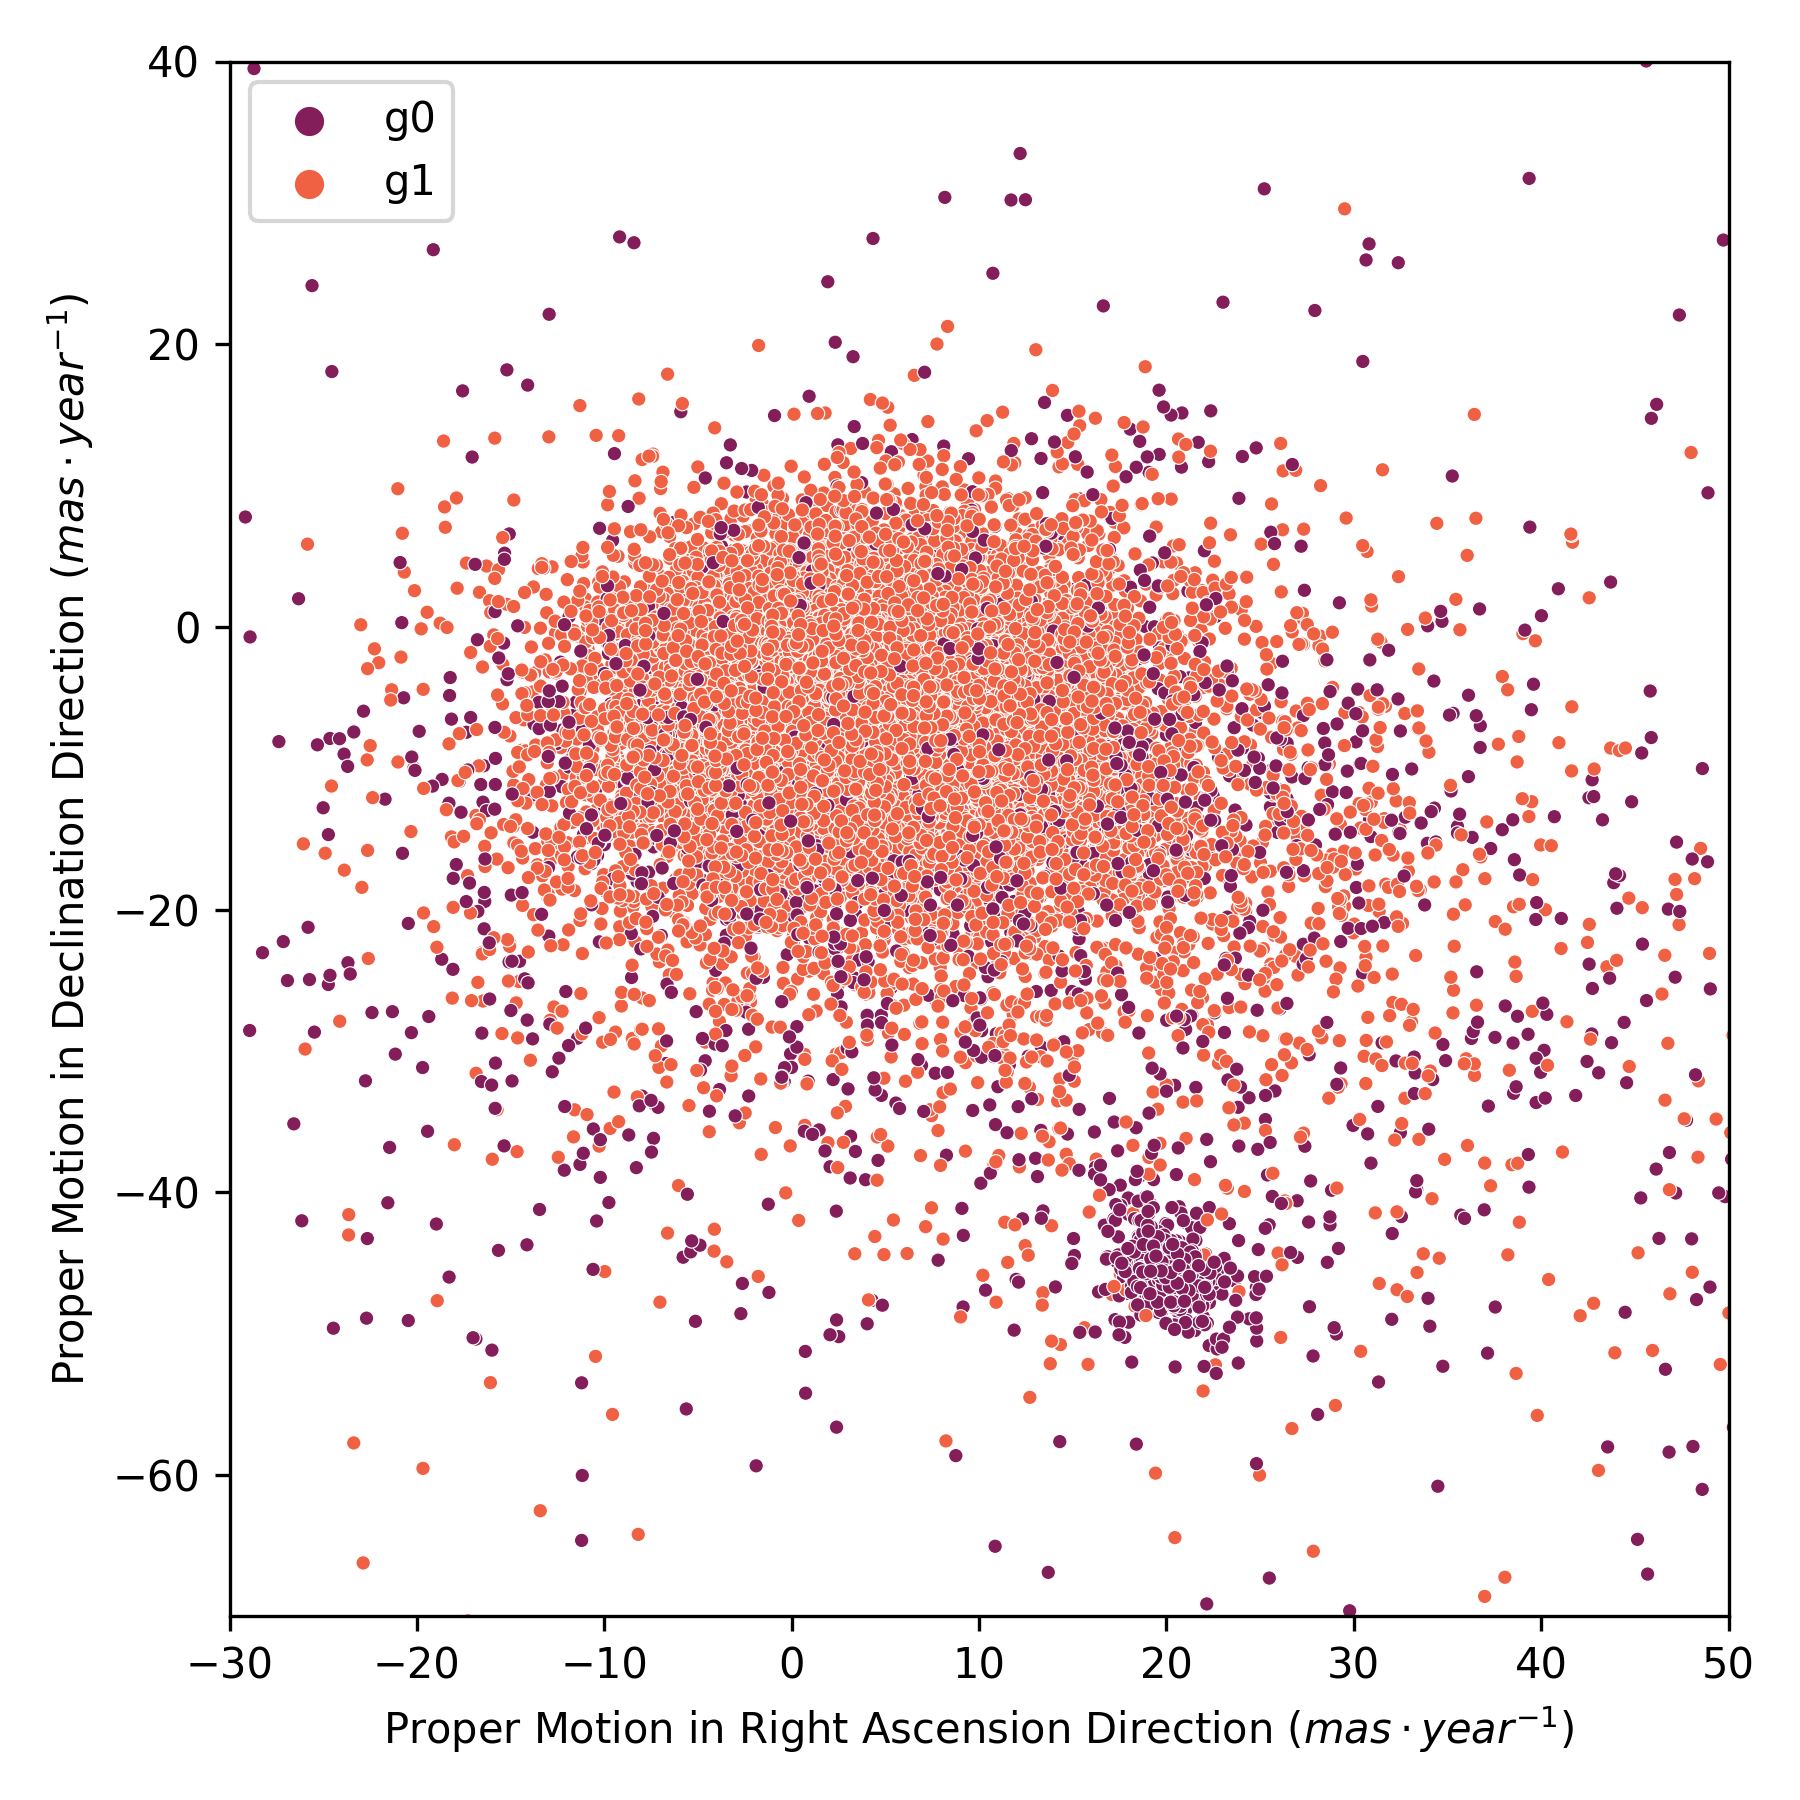
\includegraphics[width=\textwidth]{../figures/kmeans/kmeans_n2_pm_melotte_22.png}
      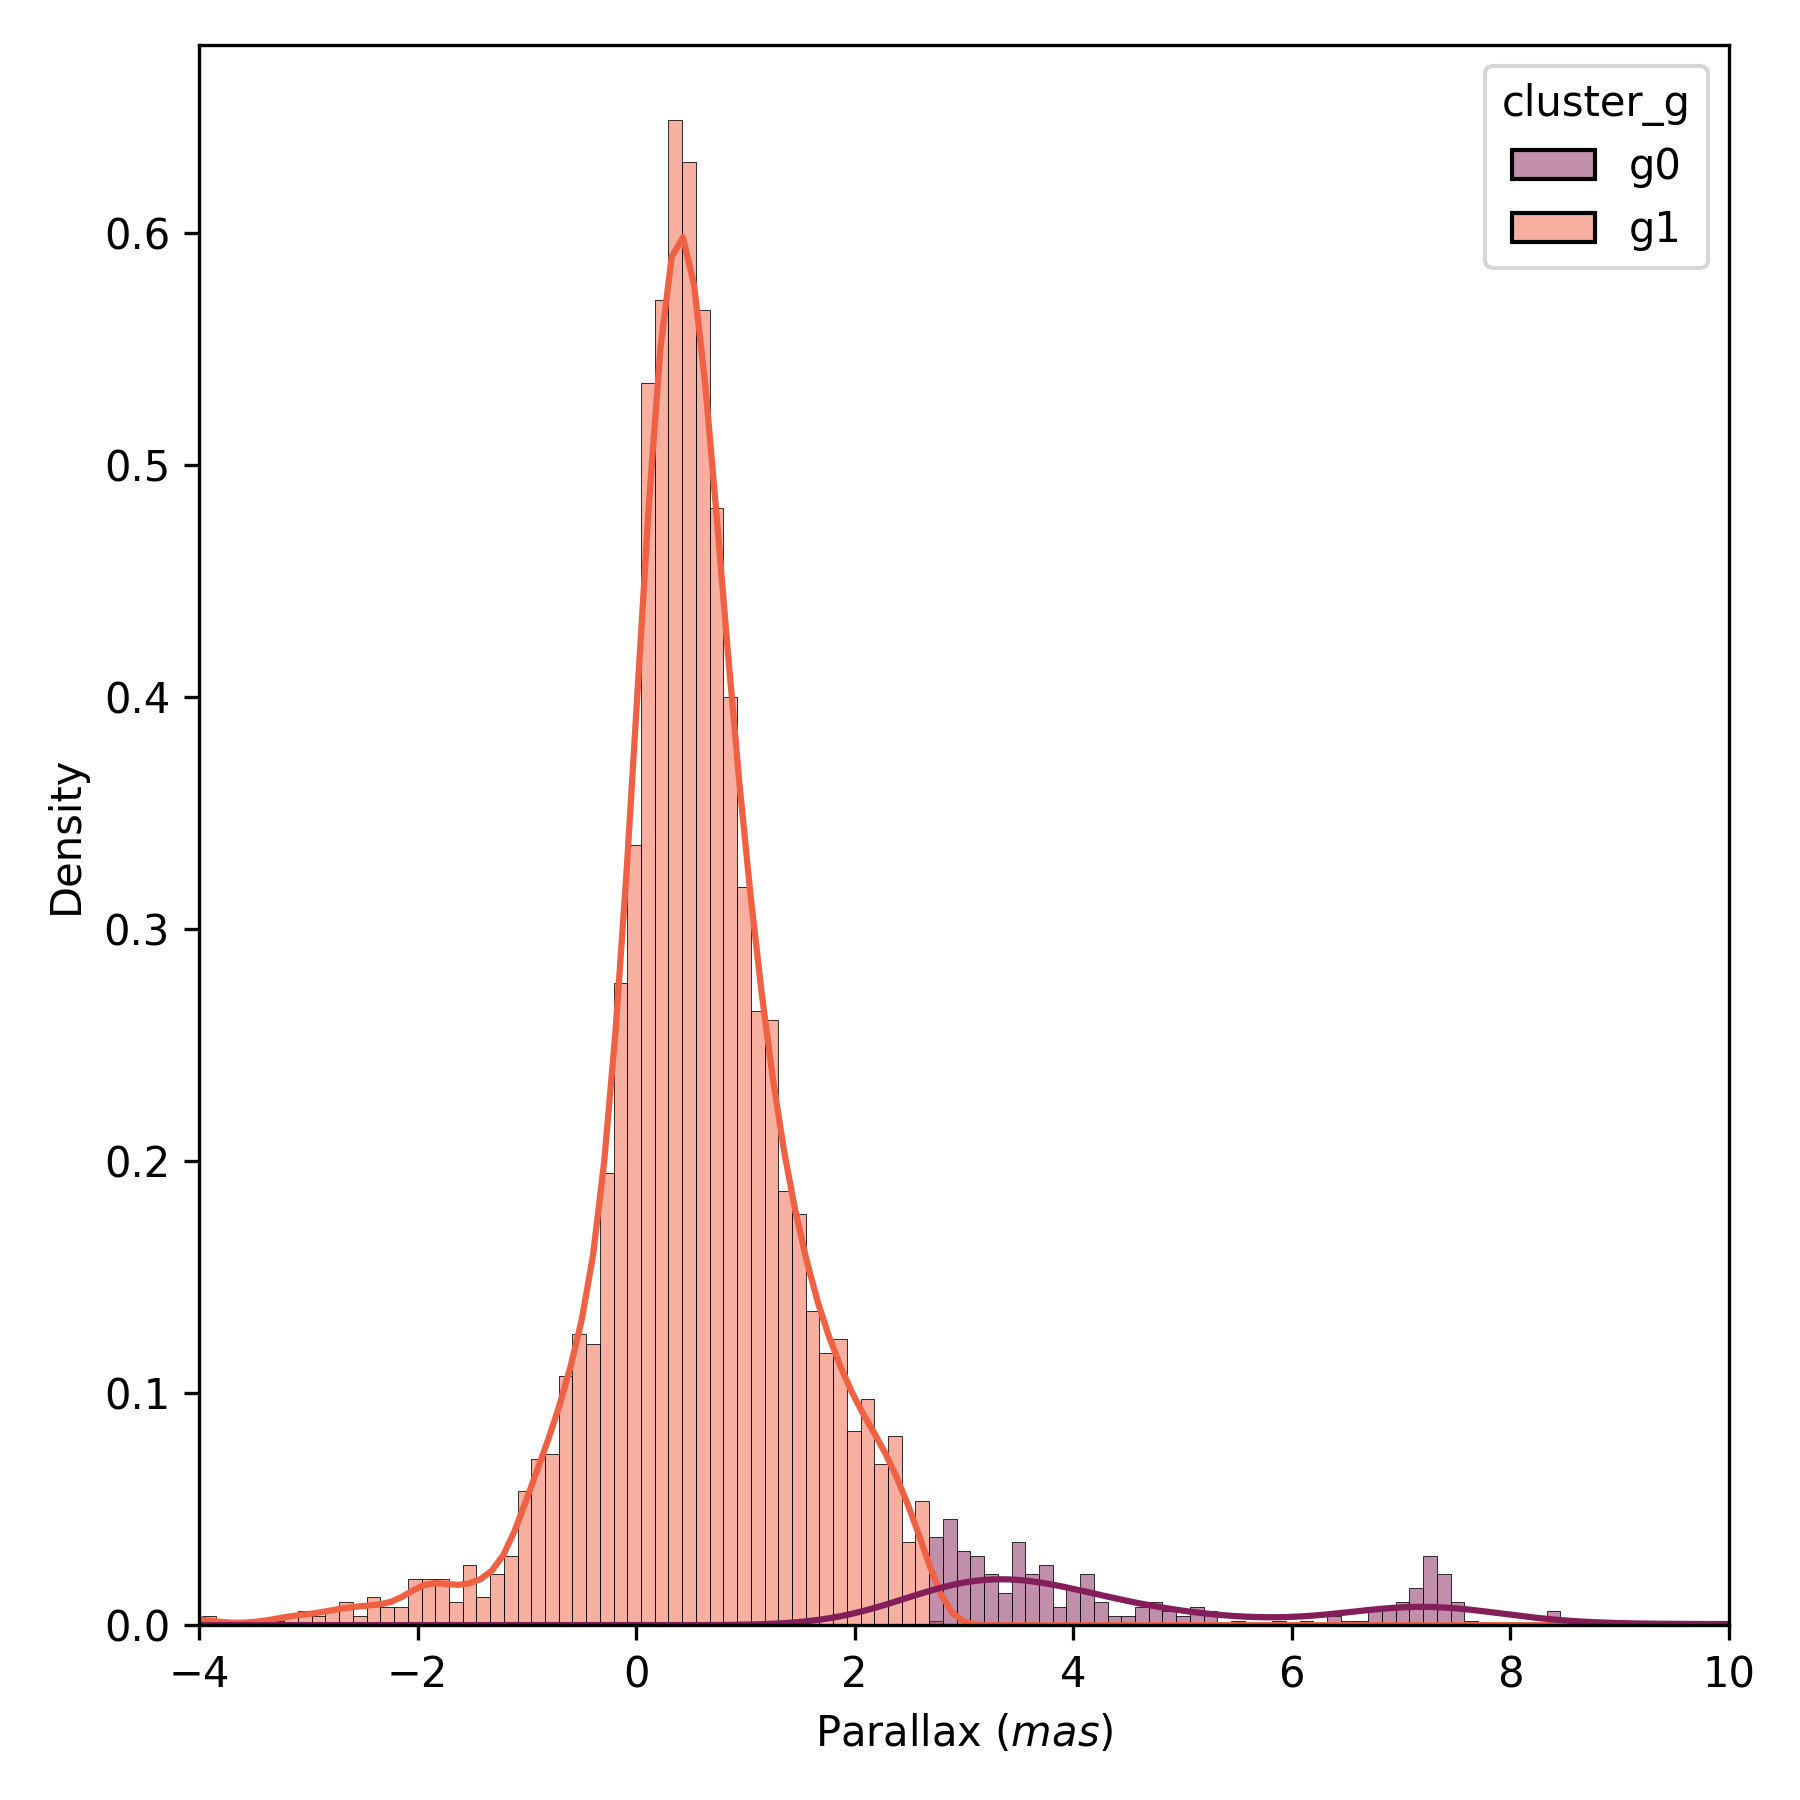
\includegraphics[width=\textwidth]{../figures/kmeans/kmeans_n2_parallax_melotte_22.png}
      \caption{N = 2}
  \end{subfigure}
  \medskip
  \begin{subfigure}[b]{0.3\textwidth}
    \centering
      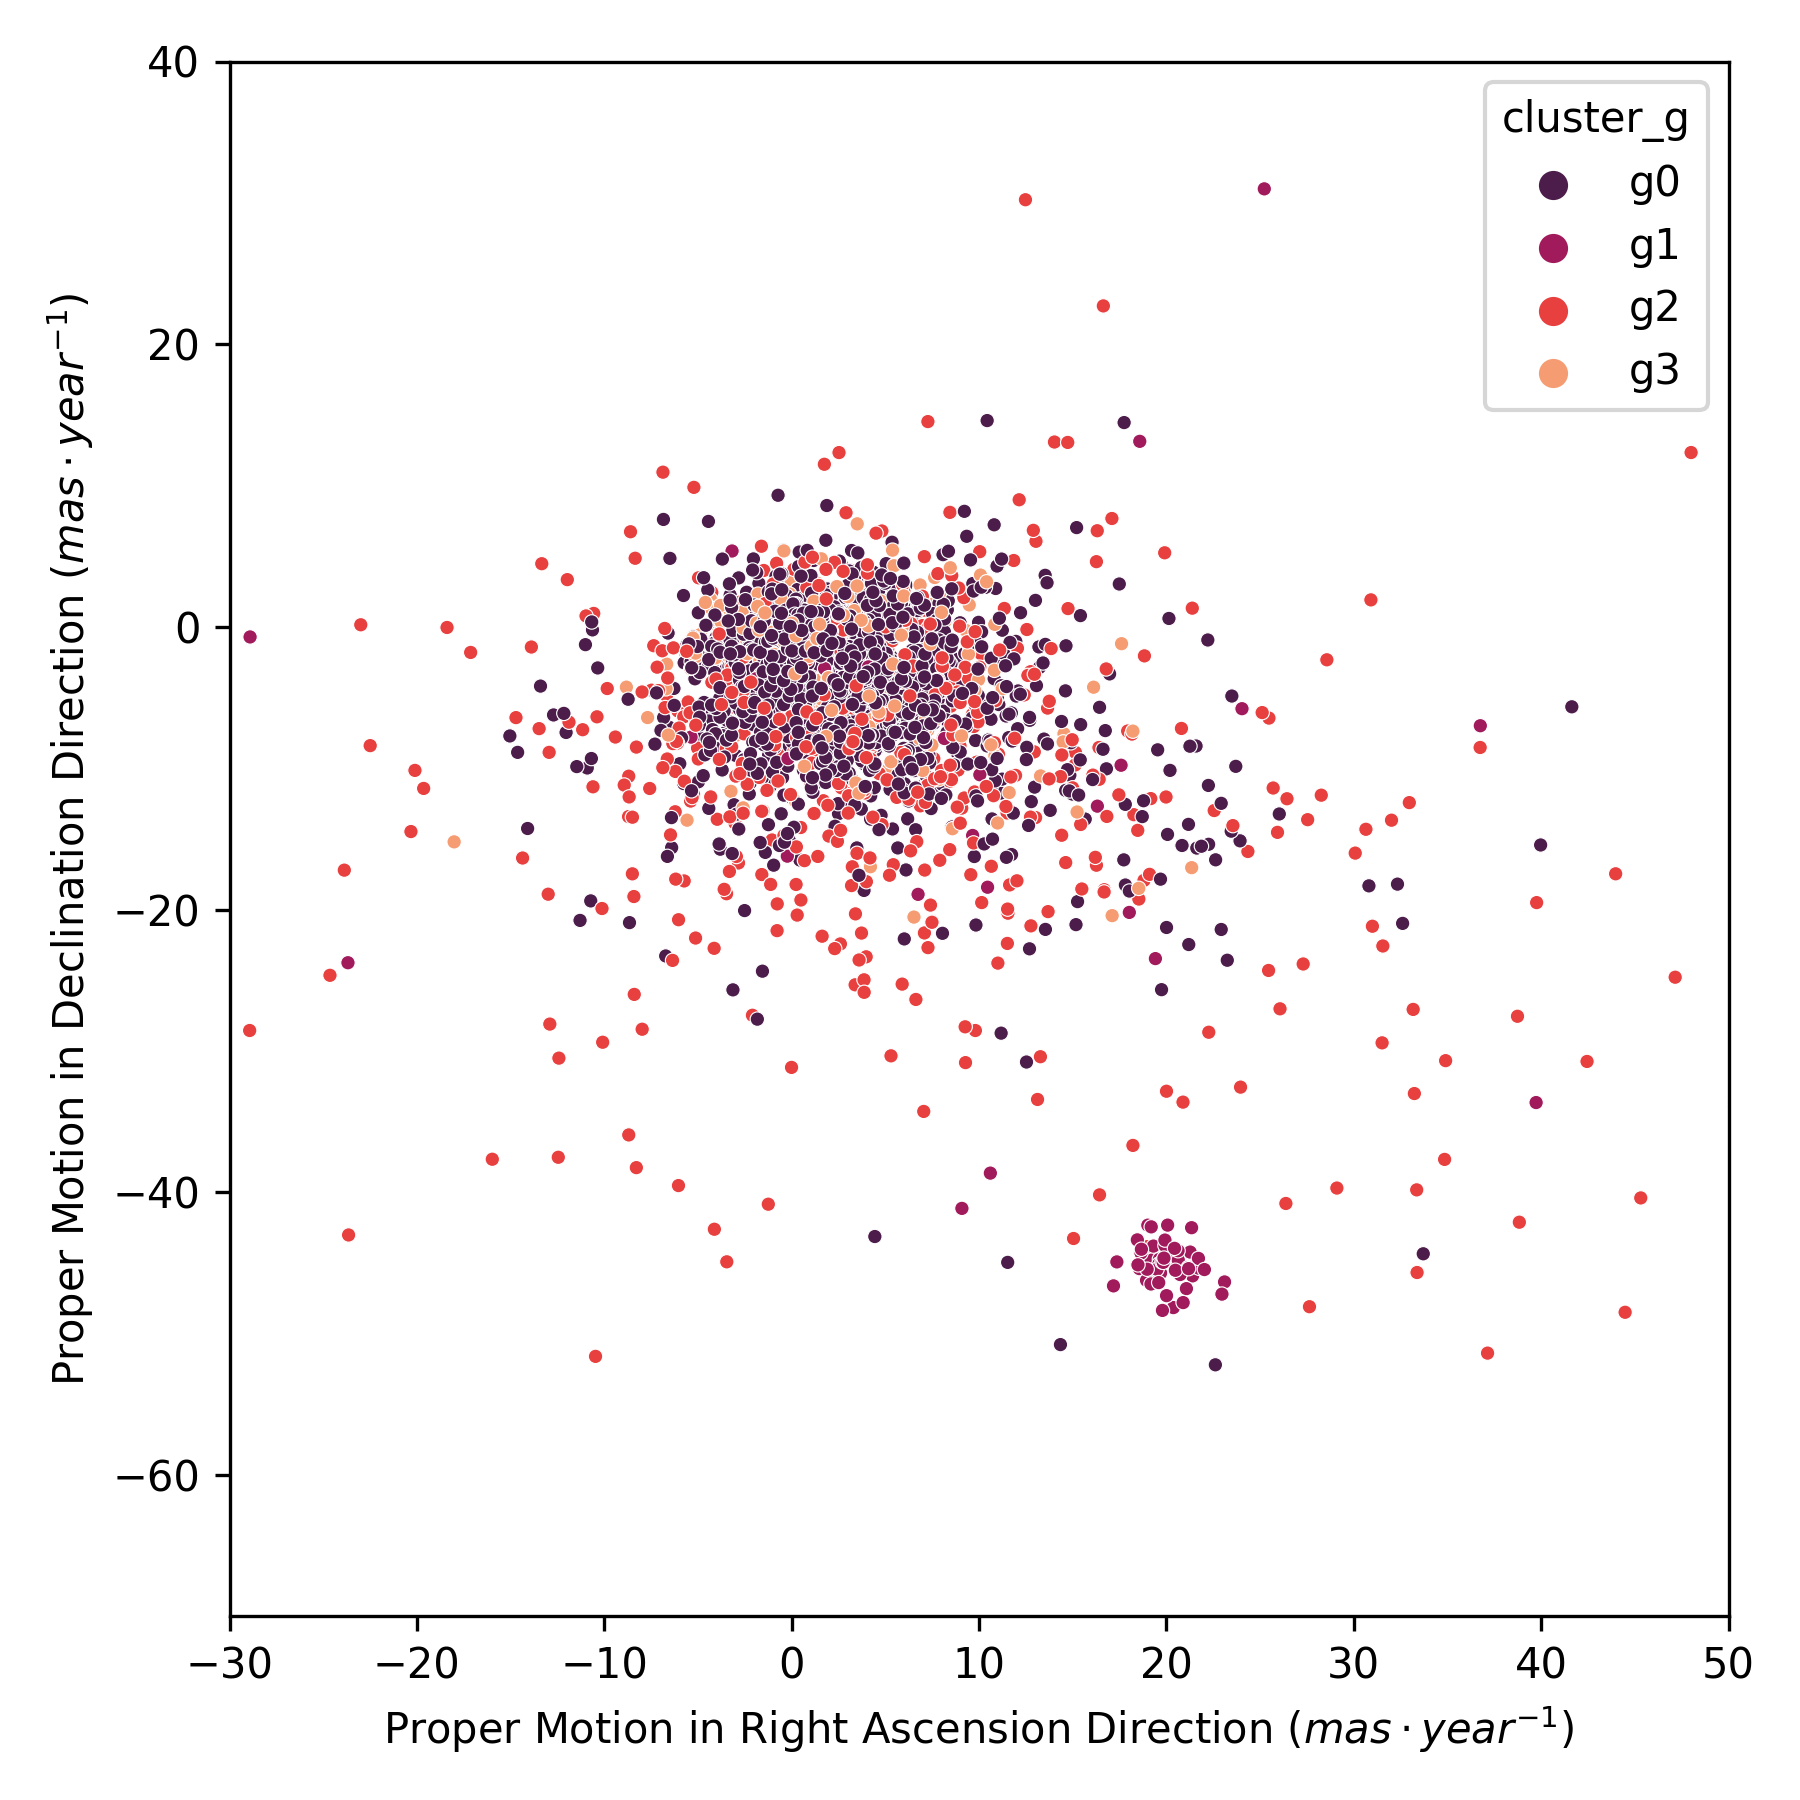
\includegraphics[width=\textwidth]{../figures/kmeans/kmeans_n5_pm_melotte_22.png}
      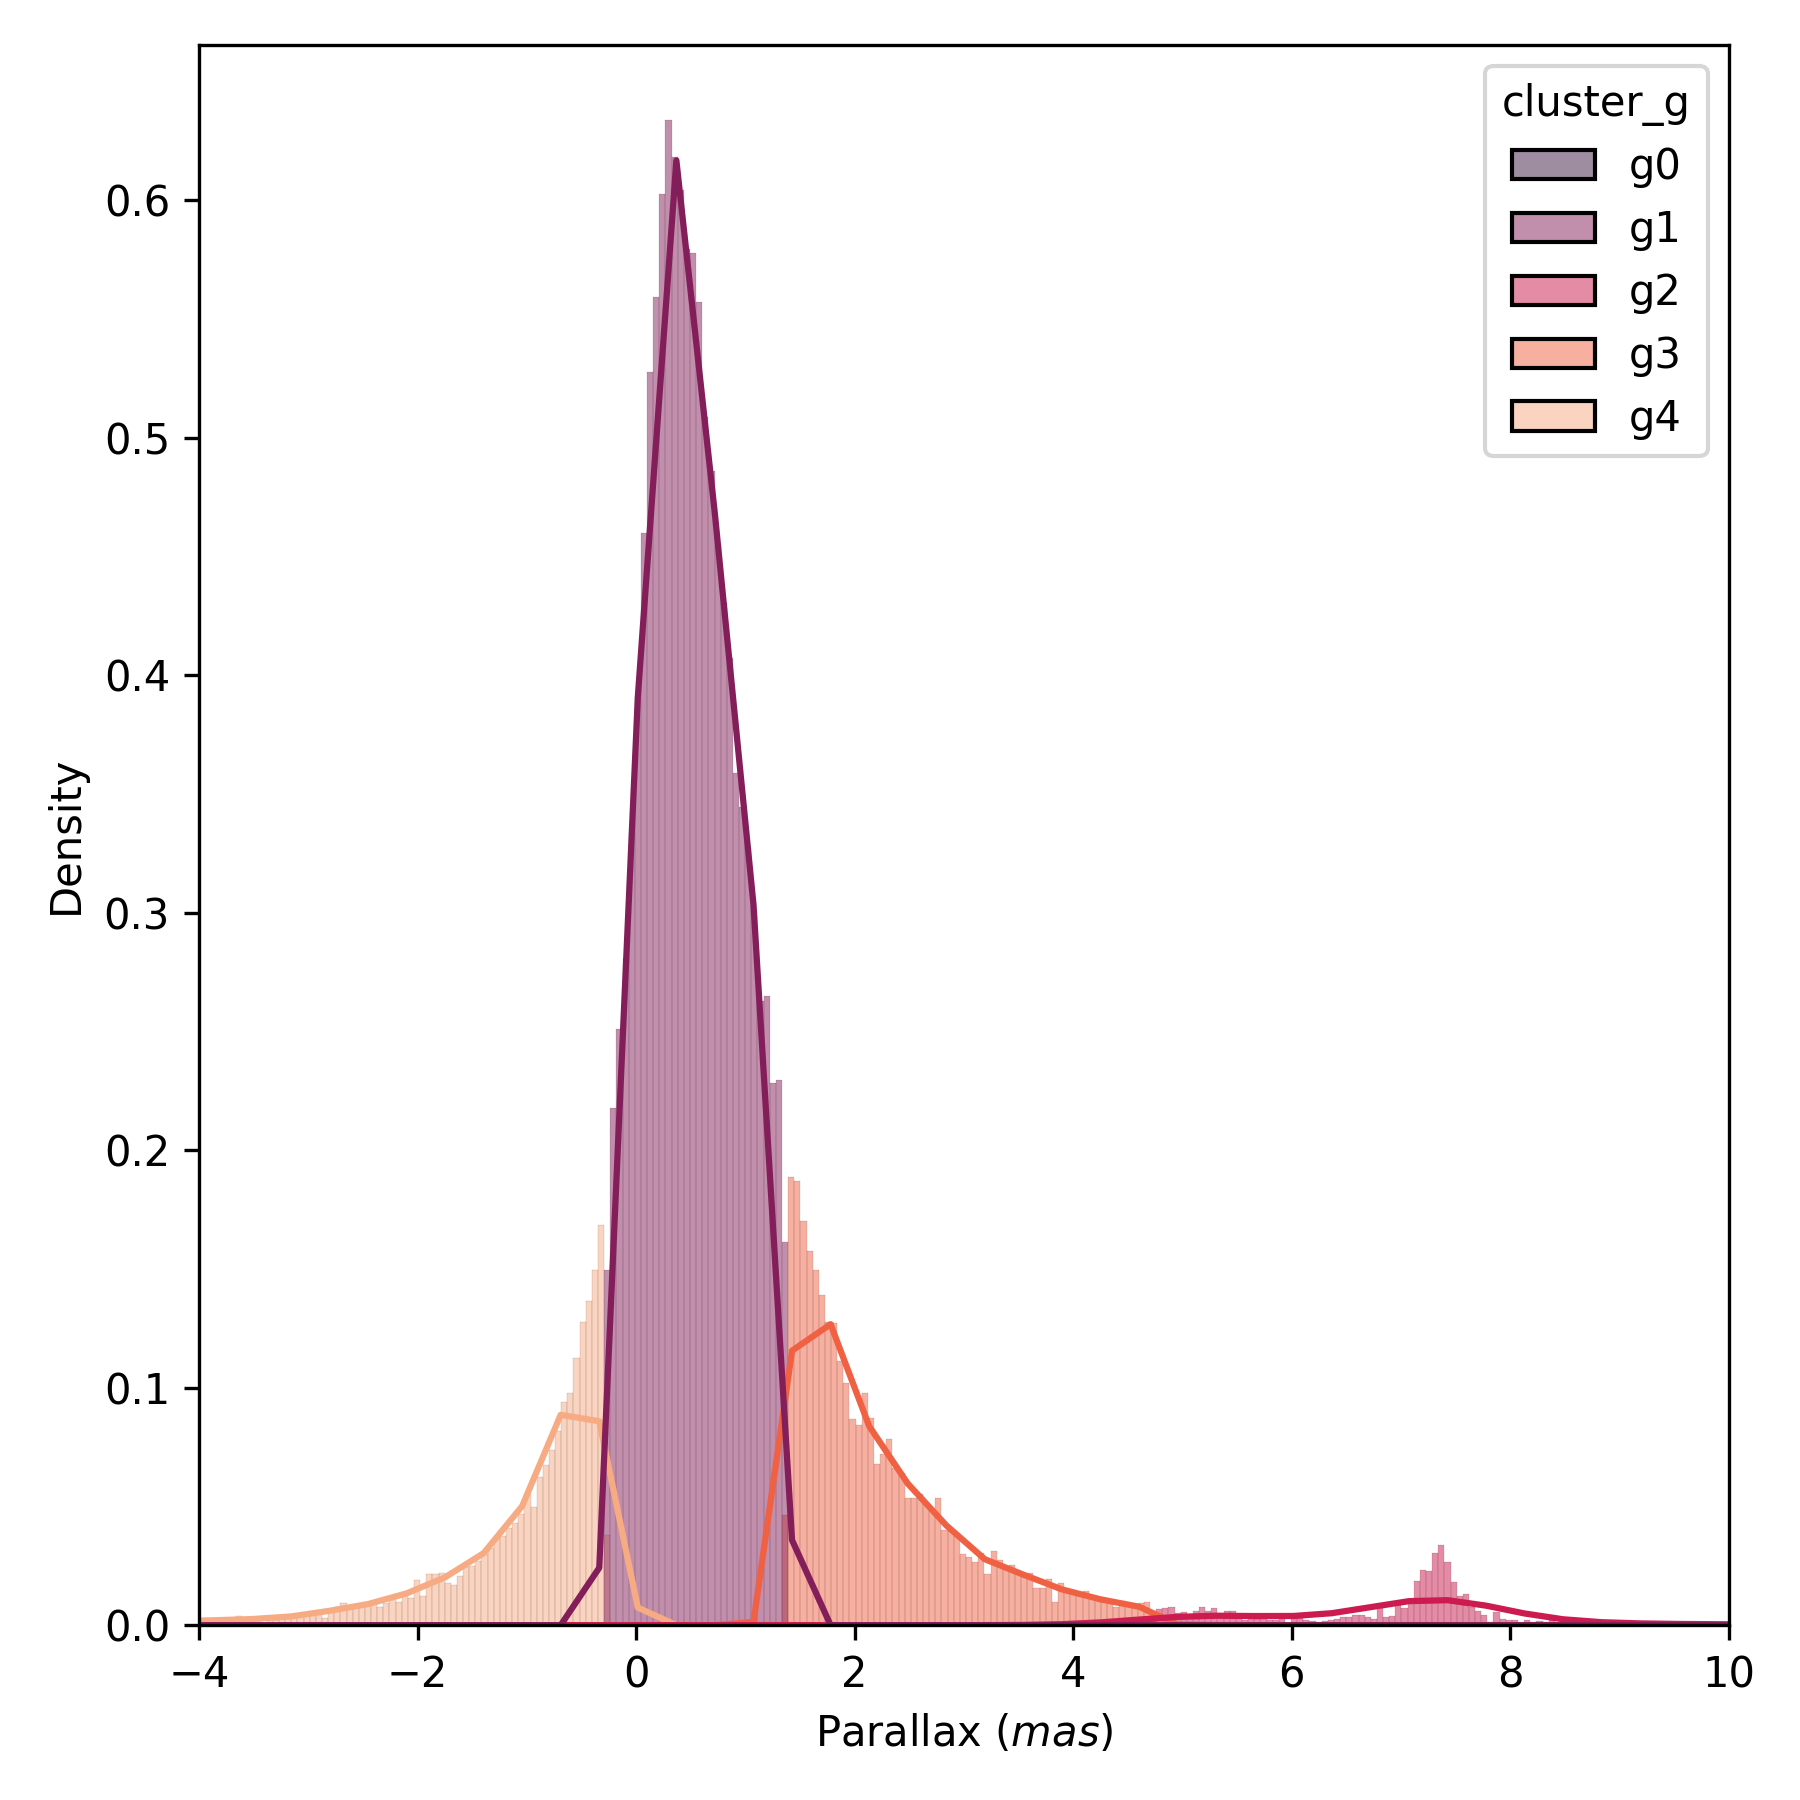
\includegraphics[width=\textwidth]{../figures/kmeans/kmeans_n5_parallax_melotte_22.png}
      \caption{N = 5}
  \end{subfigure}
  \medskip
  \begin{subfigure}[b]{0.3\textwidth}
    \centering
      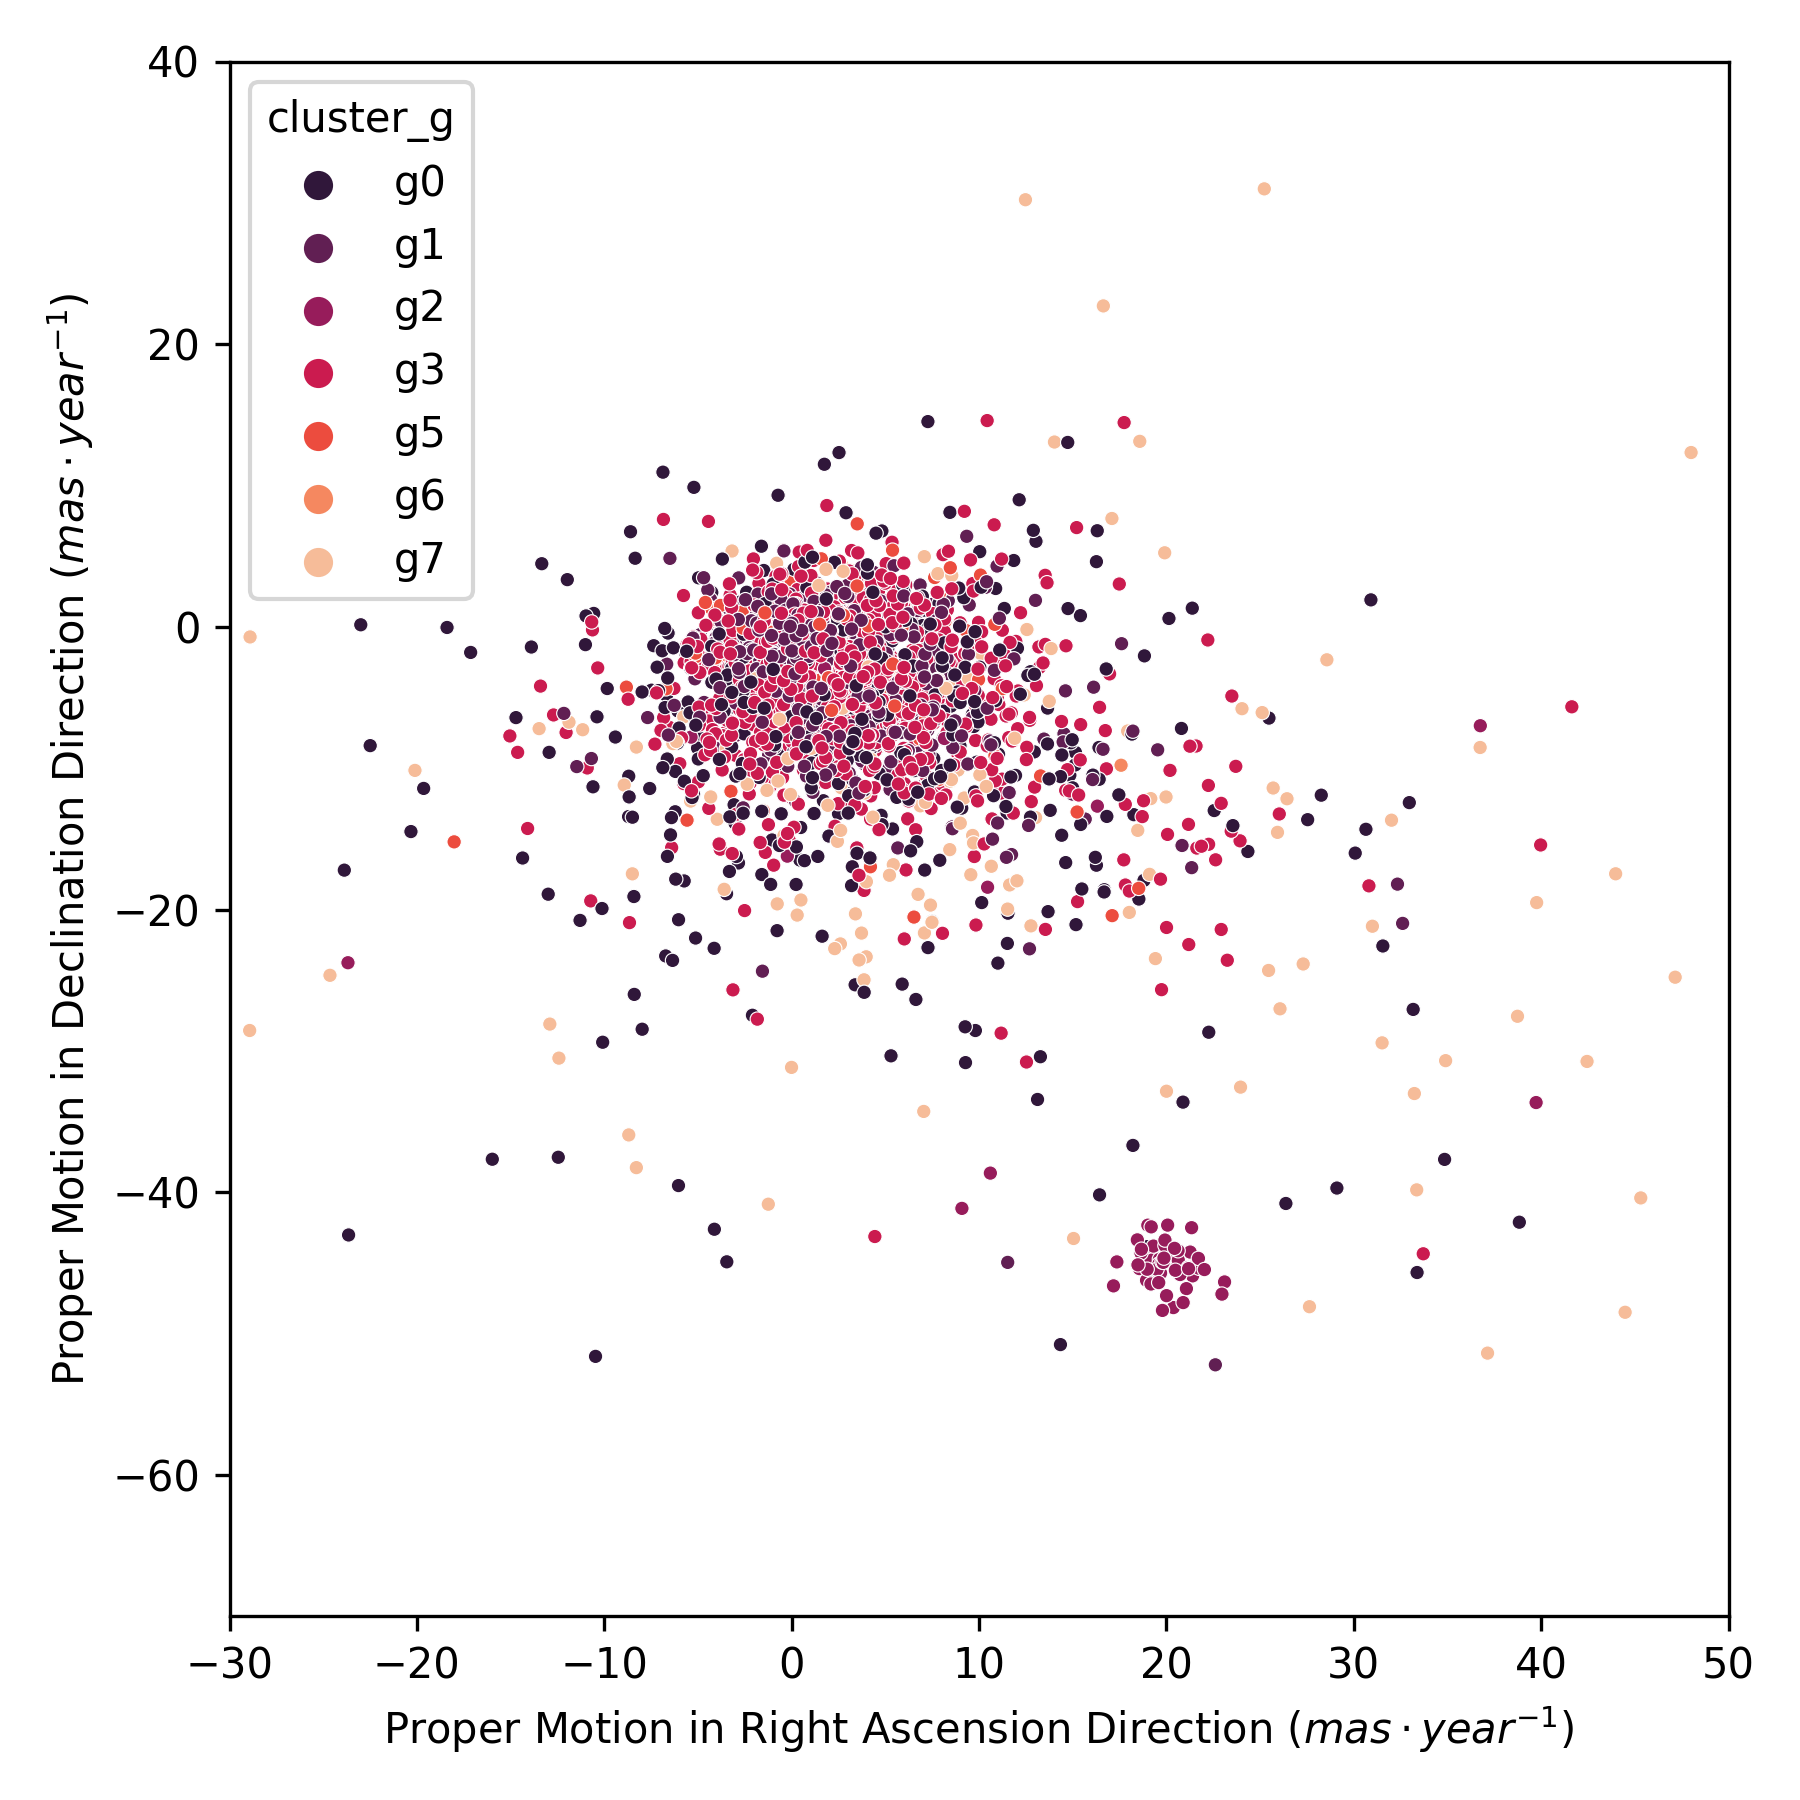
\includegraphics[width=\textwidth]{../figures/kmeans/kmeans_n8_pm_melotte_22.png}
      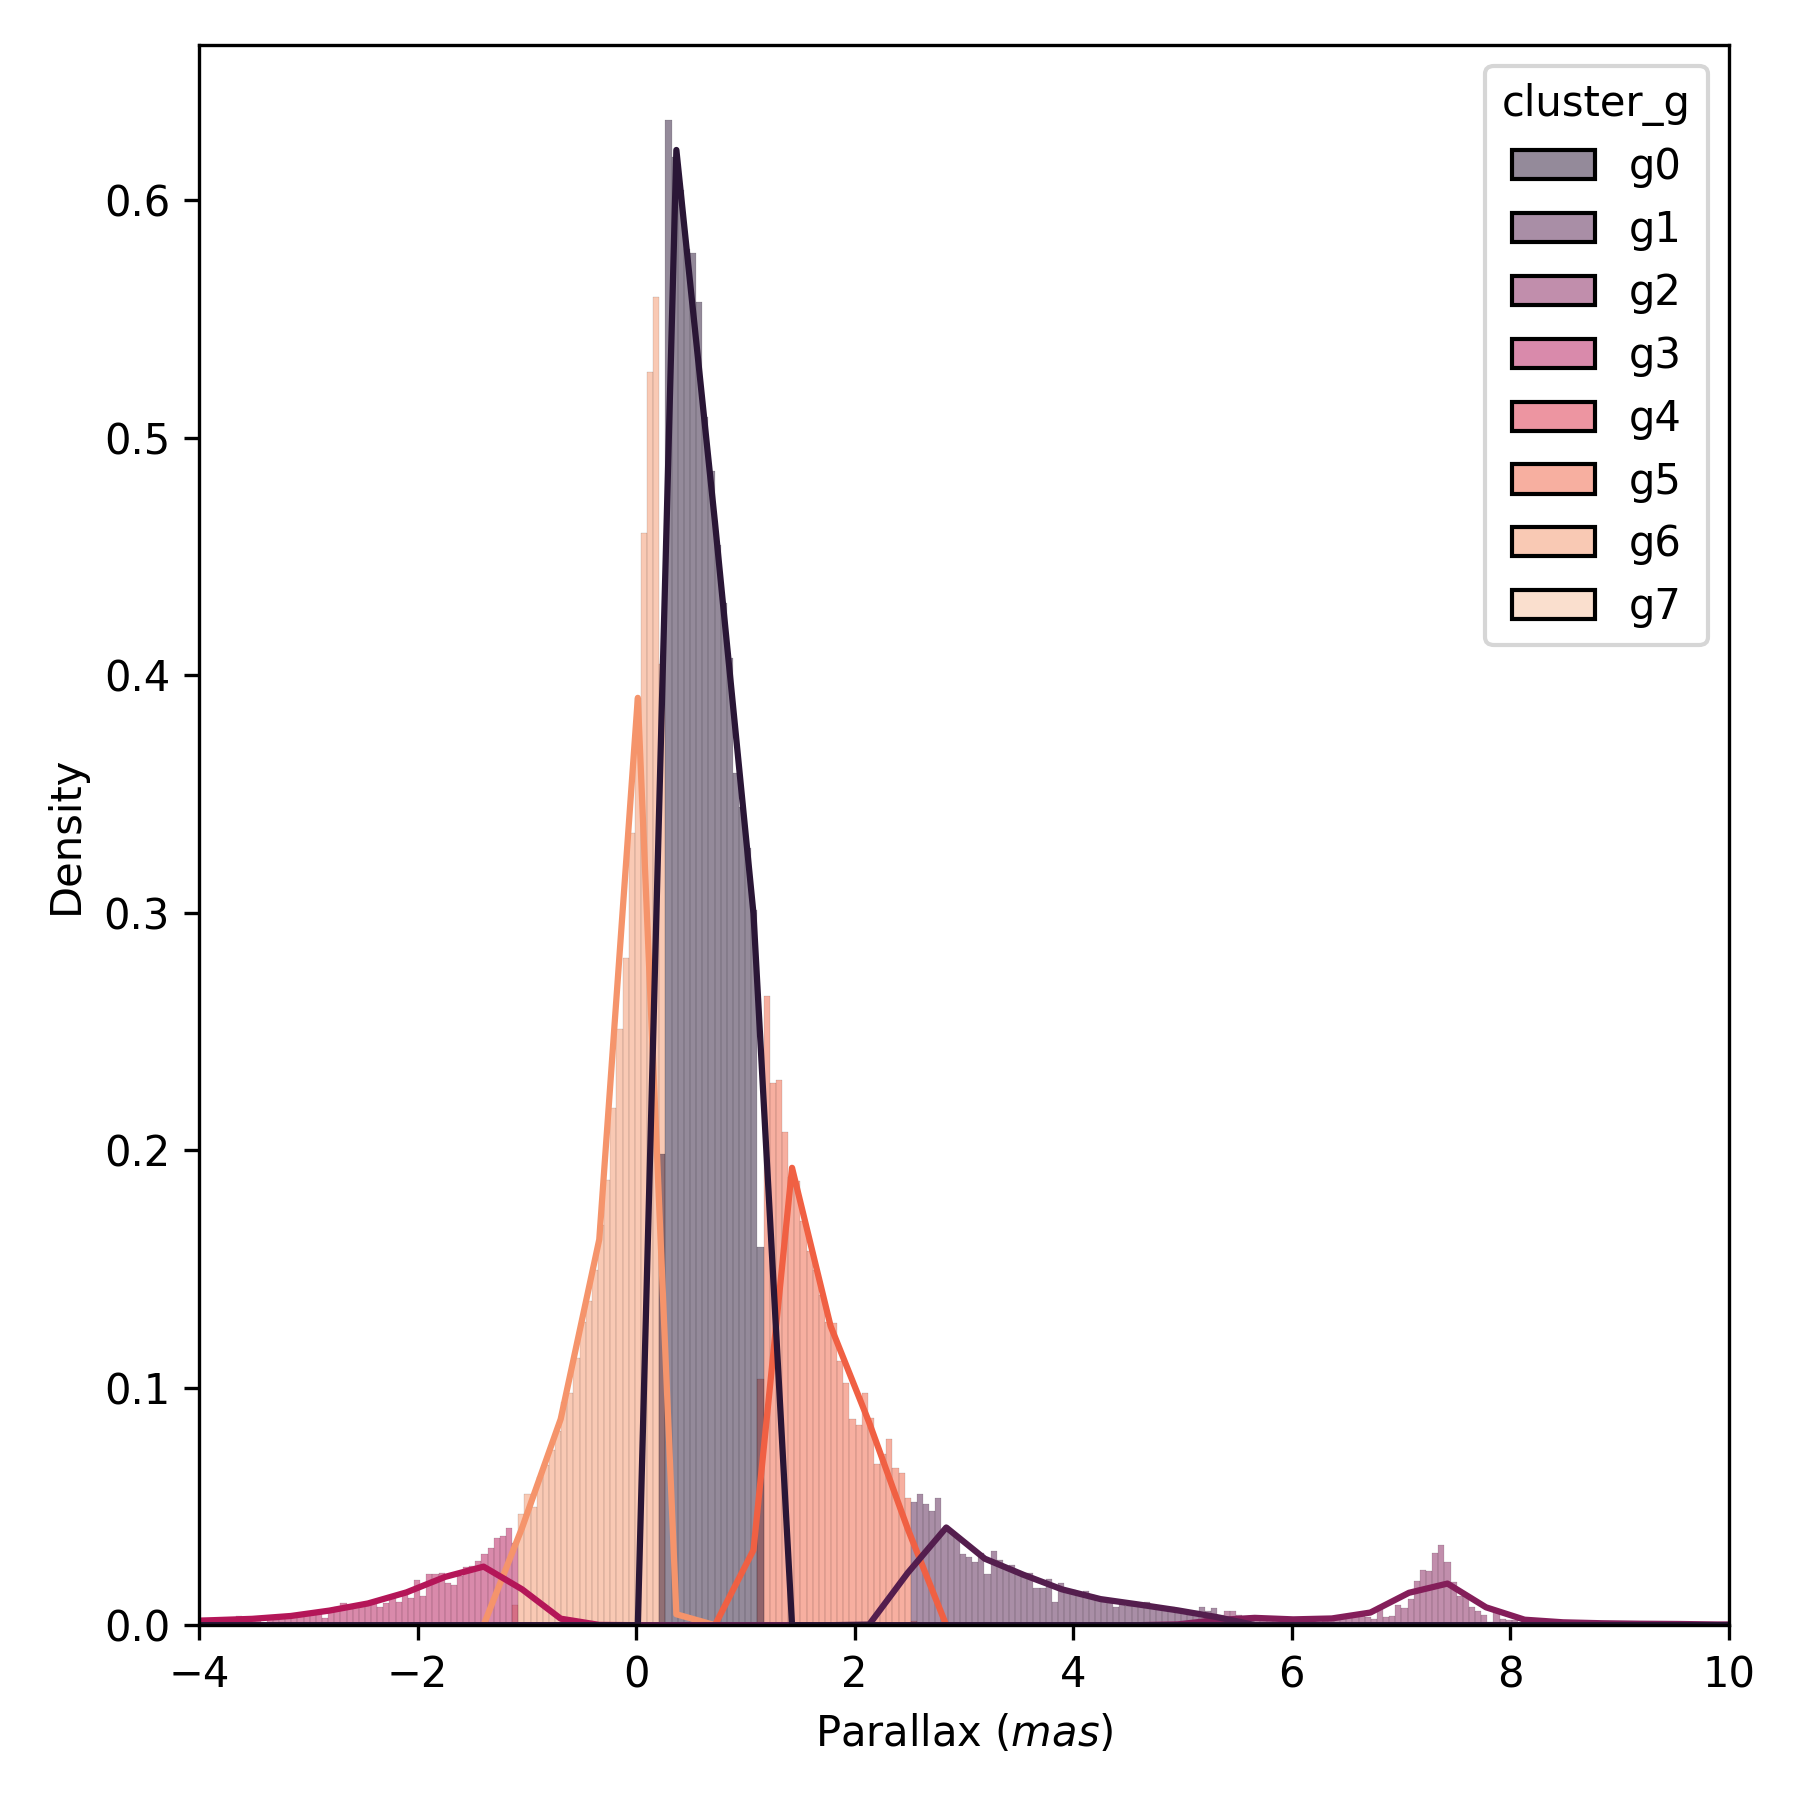
\includegraphics[width=\textwidth]{../figures/kmeans/kmeans_n8_parallax_melotte_22.png}
      \caption{N = 8}
  \end{subfigure}
  \caption{K-Means with Melotte 22}
  \label{fig:kmeans_comparisons_melotte_22}
\end{figure*}

Finally, we can refine this selection by filtering those stars which are bellow and above
the 0.10 and 0.90 quantiles for each group, respectively. That way we remove the most
doubtful values from the selection.

\paragraph{Discussion.}

Since we are looking for a single cluster, it seems reasonable to use a clustering algorithm
like K-Means to find two clusters. One for the desired OC and another for stars that do not
belong to the OC. However, the idea is not completely right. This is due to the fact that OC's
stars are surrounded by other stars with possibly similar properties. Therefore, setting the
number of clusters to two is too low to separate them properly.

Figure~\ref{fig:kmeans_comparisons_melotte_22} shows an example. It describes the results of
applying K-Means with N=2, N=5 and N=8 in Melotte 22. As we can see, large values of the number
of clusters allow us to isolate more accurately the resonance in parallax at \(\approx 7.3mas\).

The disadvantage is that it forms more groups of stars, which complicates the task of finding the
desired OC, since we would like to get just two groups. Therefore, with a K-Means we have to find
a way to set the right value for the number of clusters to isolate the searched cluster without
creating too many groups. To solve this issue, we can try to estimate the best number of clusters
by using the \emph{silhouette score}~\cite{rousseeuw1987silhouettes}.

K-Means does a good job making an initial clustering. However, too many clusters arise
from this characterization and the OC is still polluted with stars that do not belong to it.
Moreover, we would like to reduce the amount of clusters too.

\section{Results}
\label{sec:results}

%% Comparación con K-Means, DEC y DEC filter
\begin{figure*}[!htbp]
  \centering
  \begin{subfigure}[b]{0.3\textwidth}
    \centering
      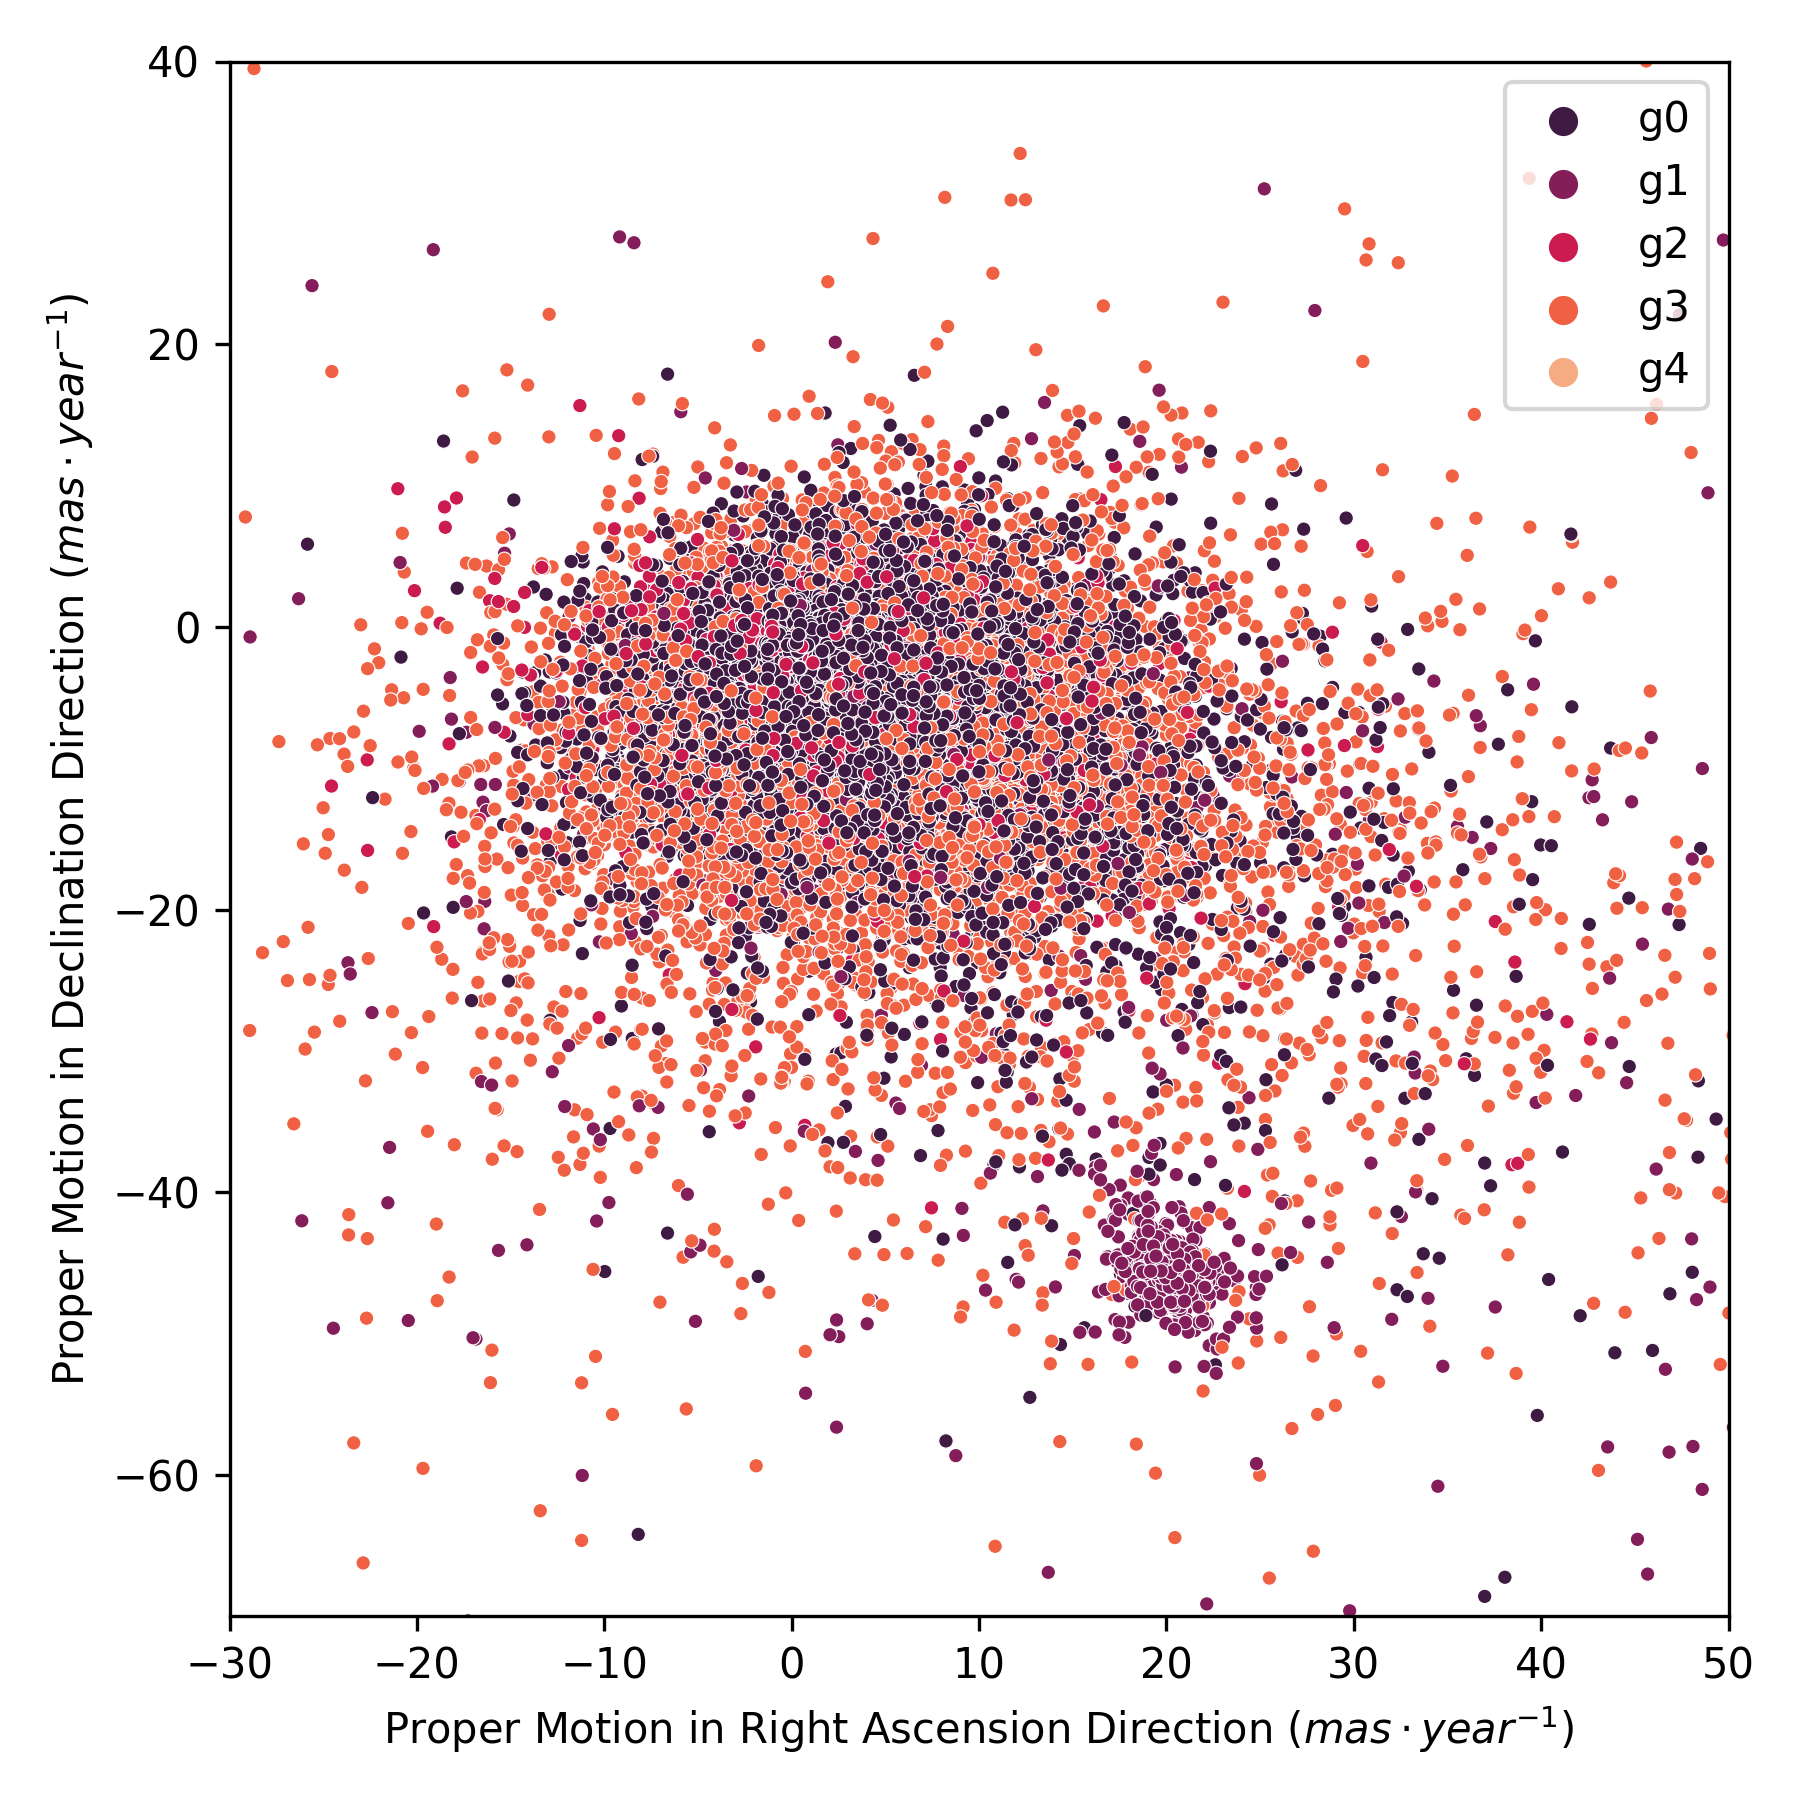
\includegraphics[width=\textwidth]{../figures/melotte_22/kmeans_pm_melotte_22.png}
      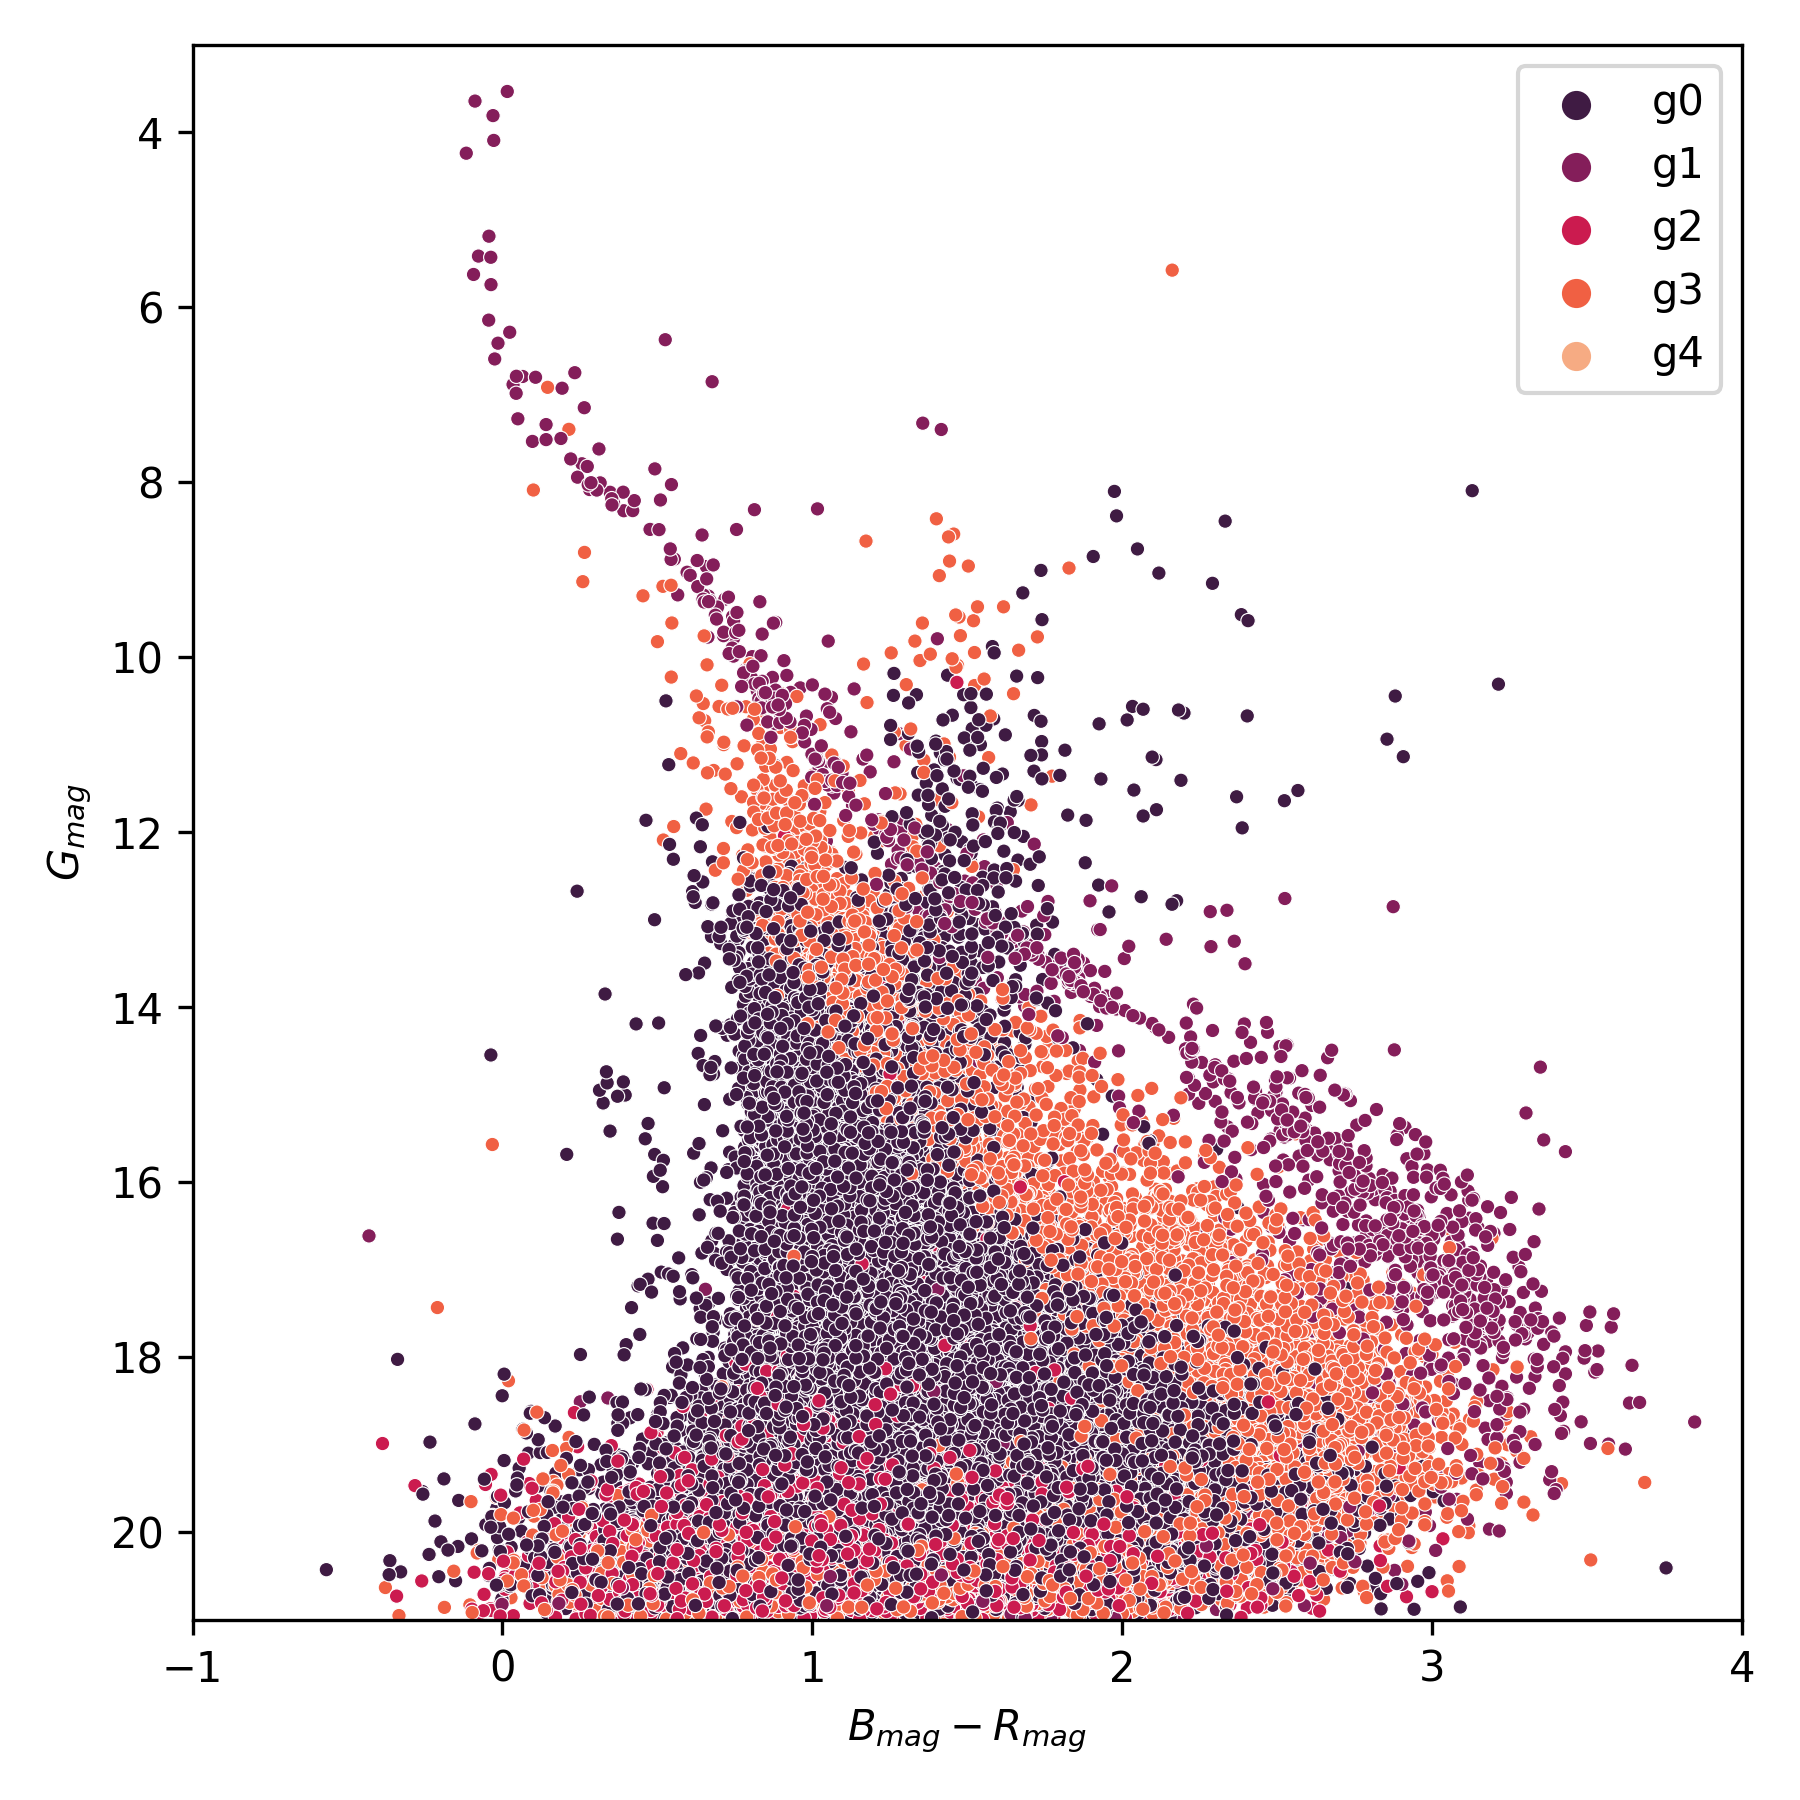
\includegraphics[width=\textwidth]{../figures/melotte_22/kmeans_hr_diagram_melotte_22.png}
      \caption{K-Means}
  \end{subfigure}
  \medskip
  \begin{subfigure}[b]{0.3\textwidth}
    \centering
      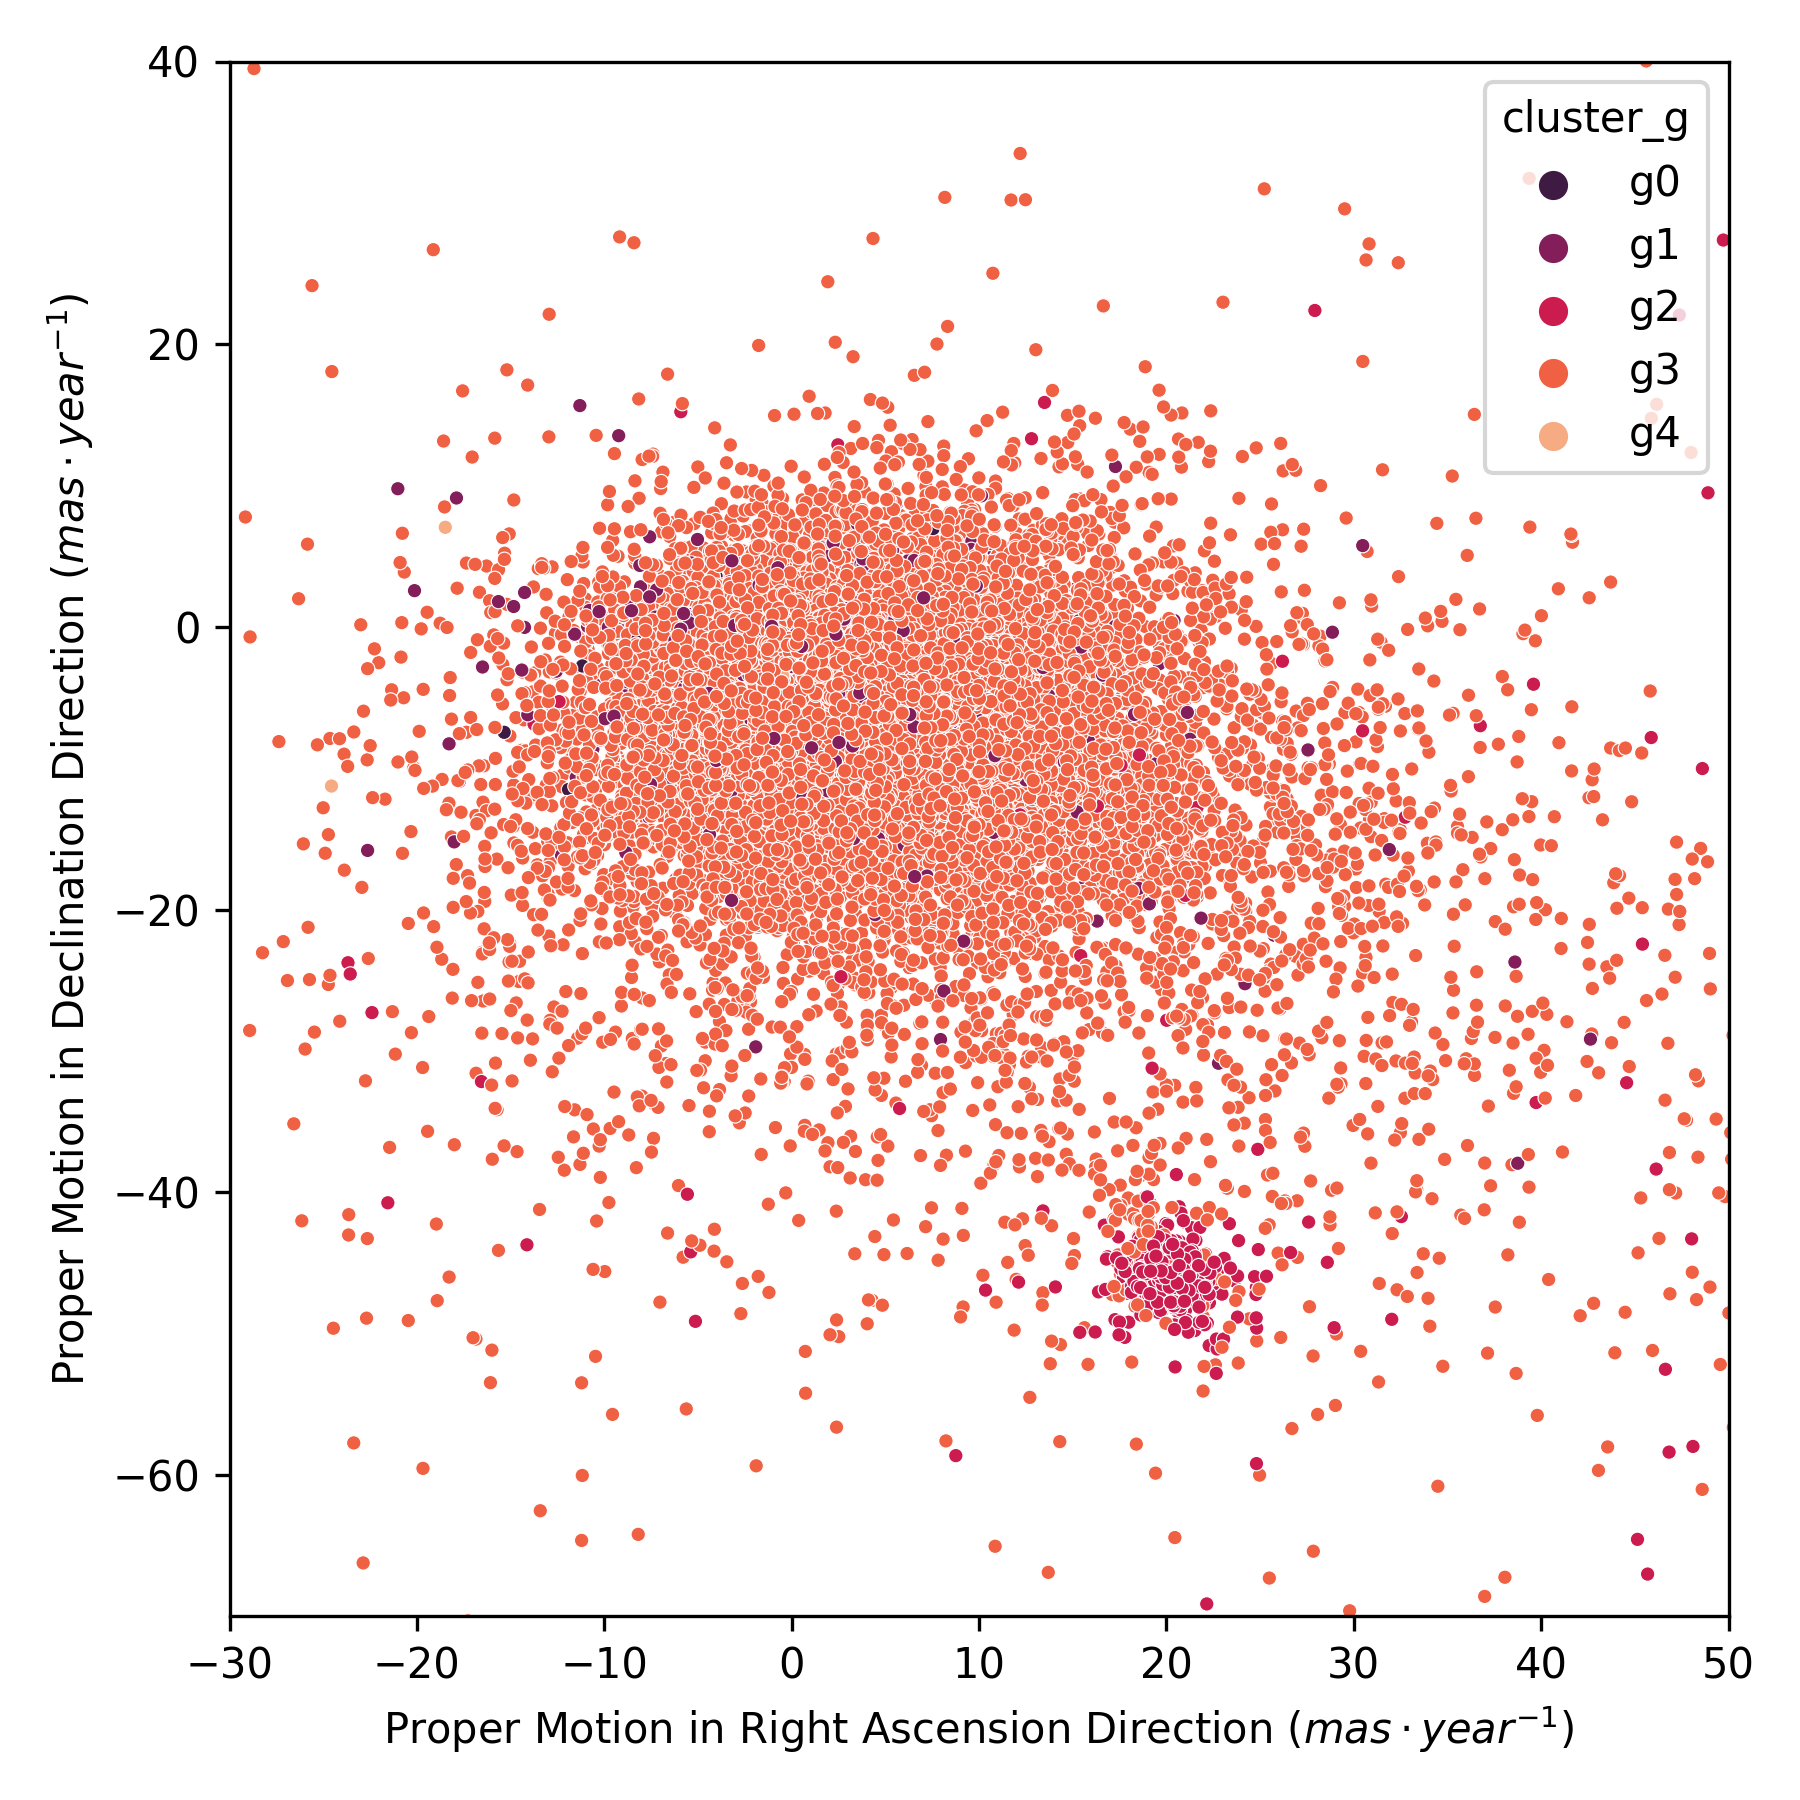
\includegraphics[width=\textwidth]{../figures/melotte_22/dec_pm_melotte_22.png}
      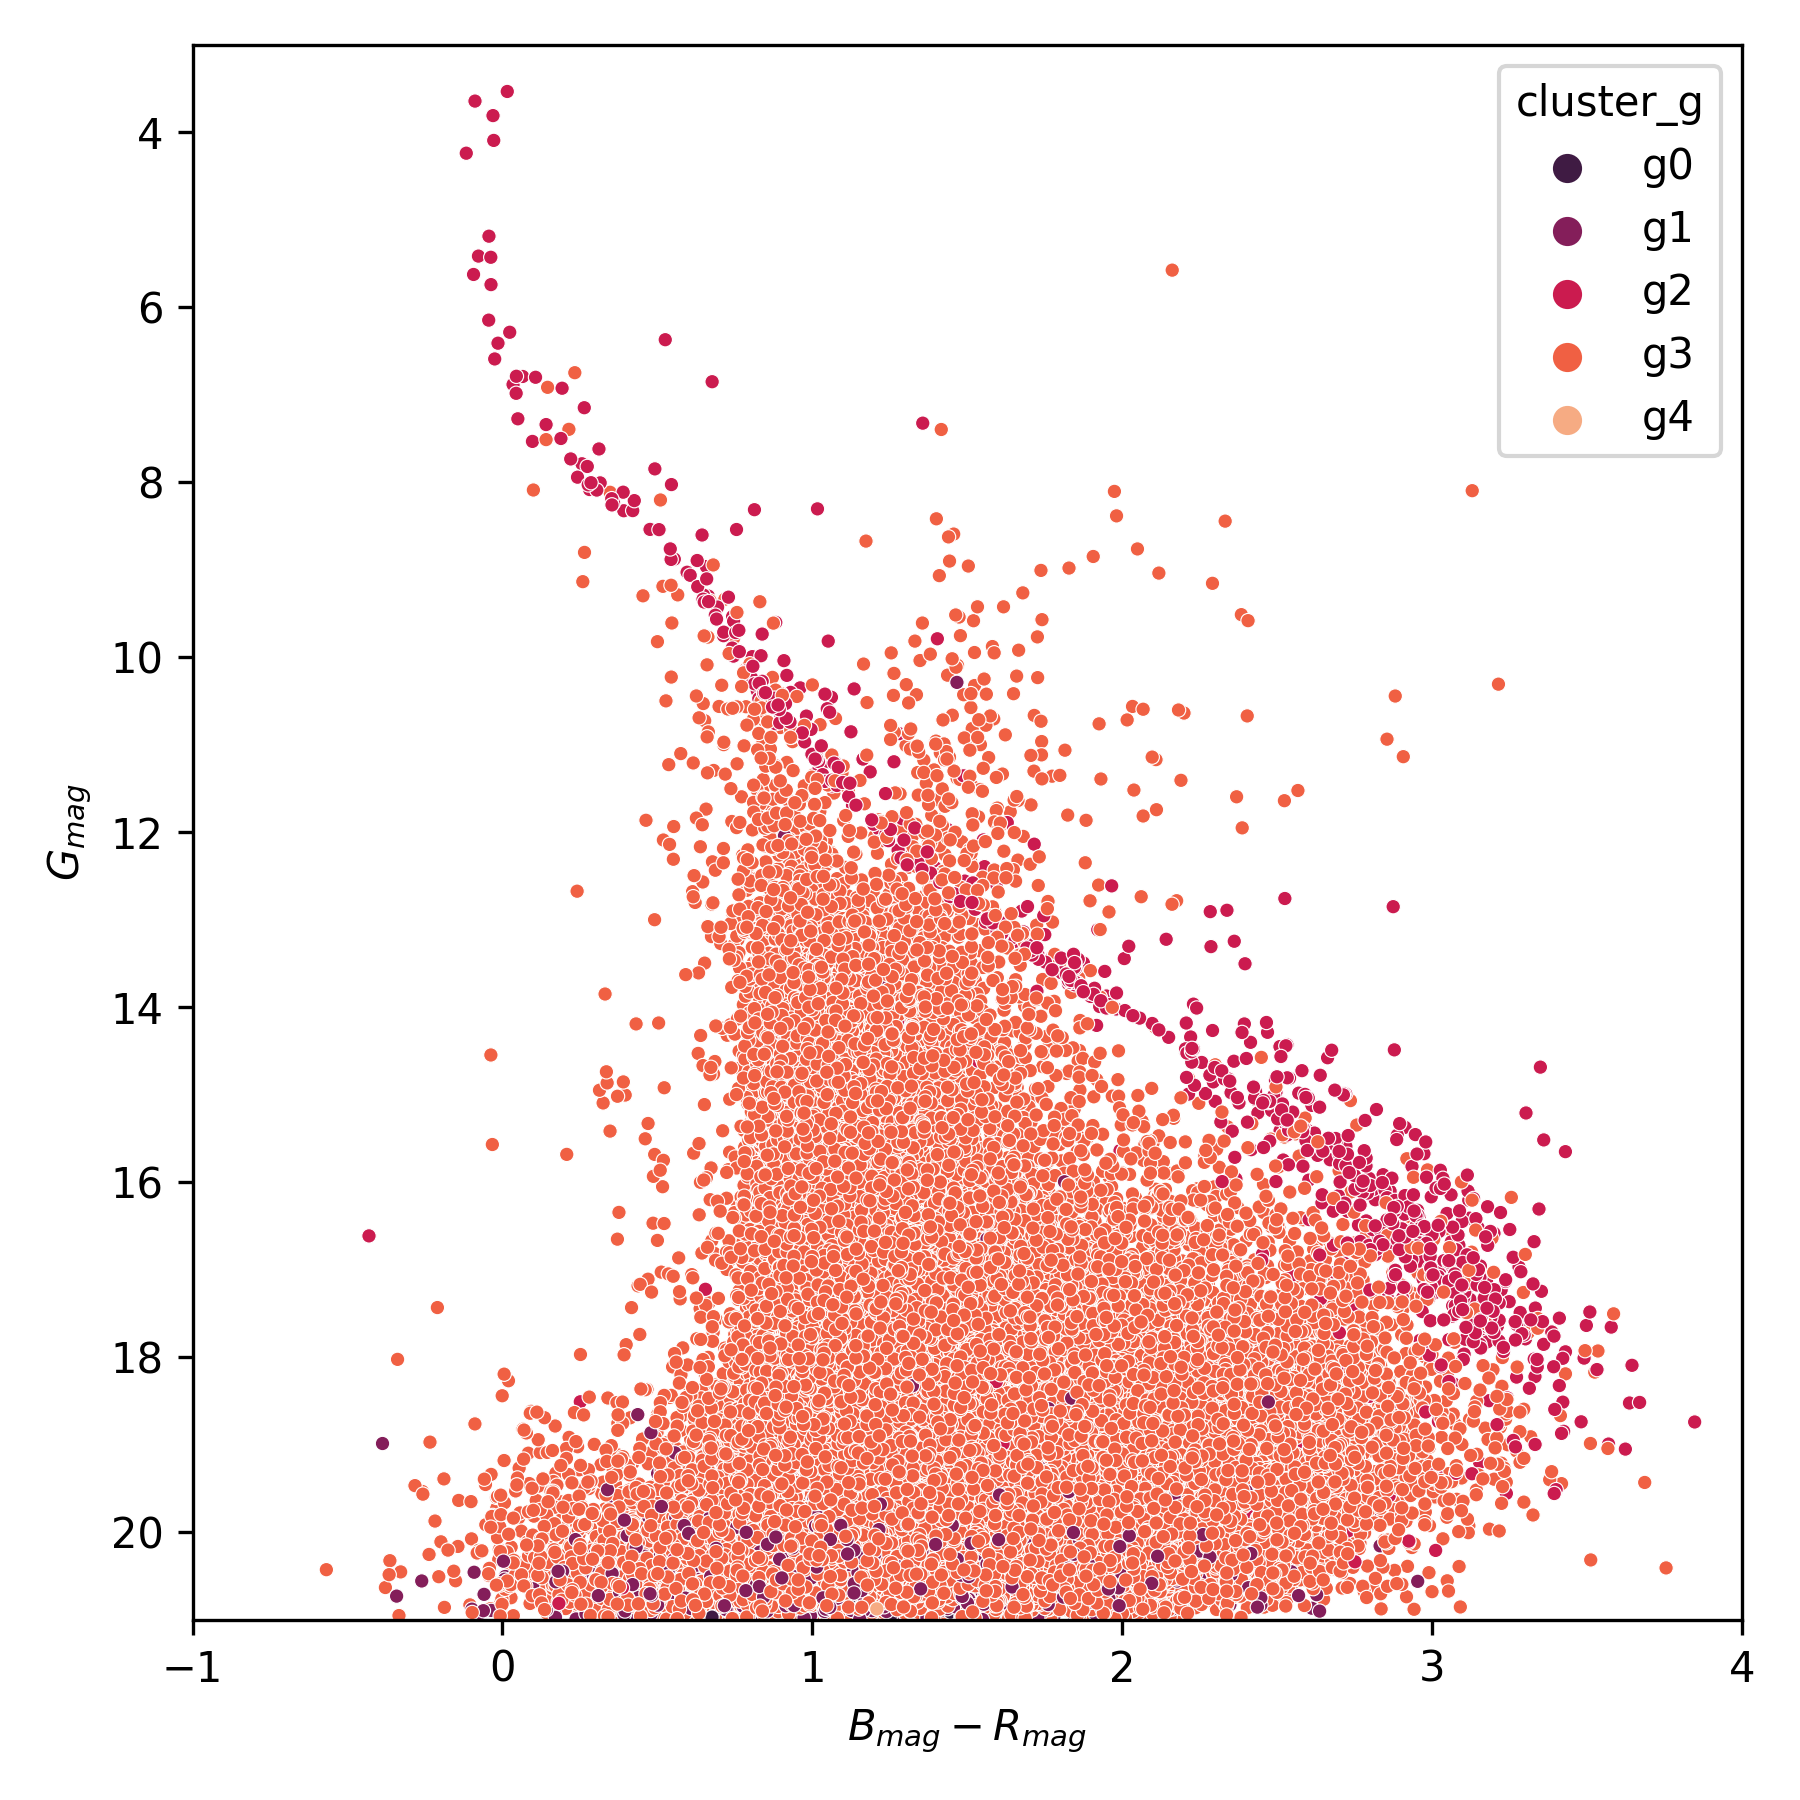
\includegraphics[width=\textwidth]{../figures/melotte_22/dec_hr_diagram_melotte_22.png}
      \caption{DEC}
  \end{subfigure}
  \medskip
  \begin{subfigure}[b]{0.3\textwidth}
    \centering
      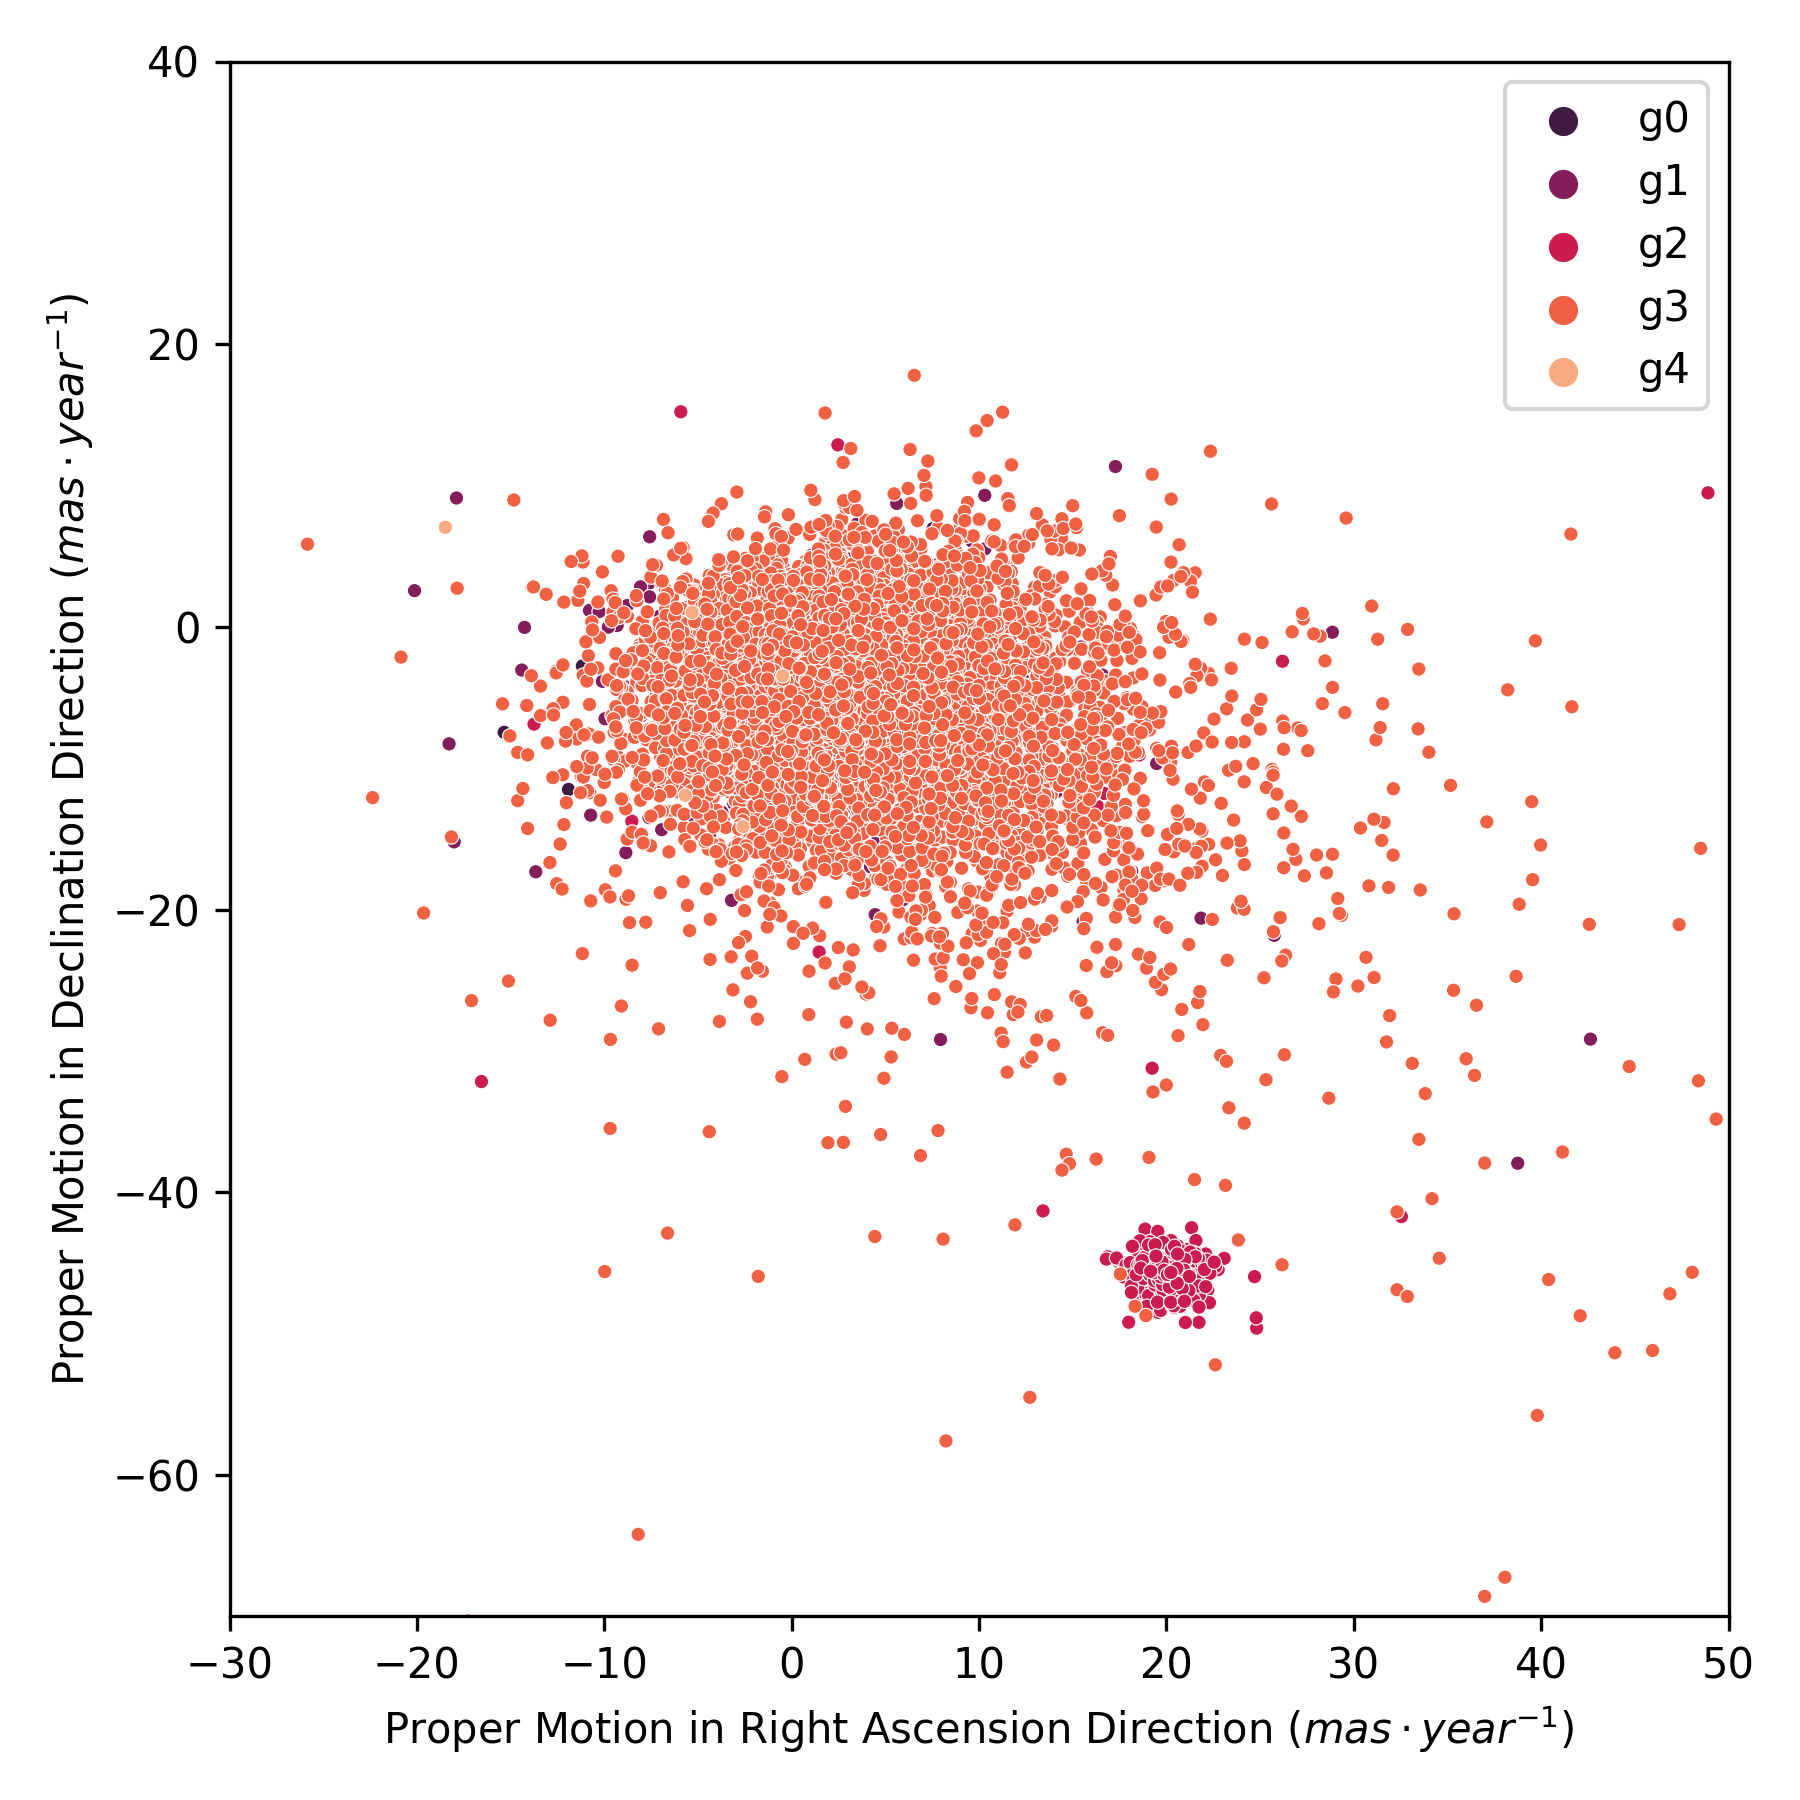
\includegraphics[width=\textwidth]{../figures/melotte_22/dec_pm_filtered_melotte_22.png}
      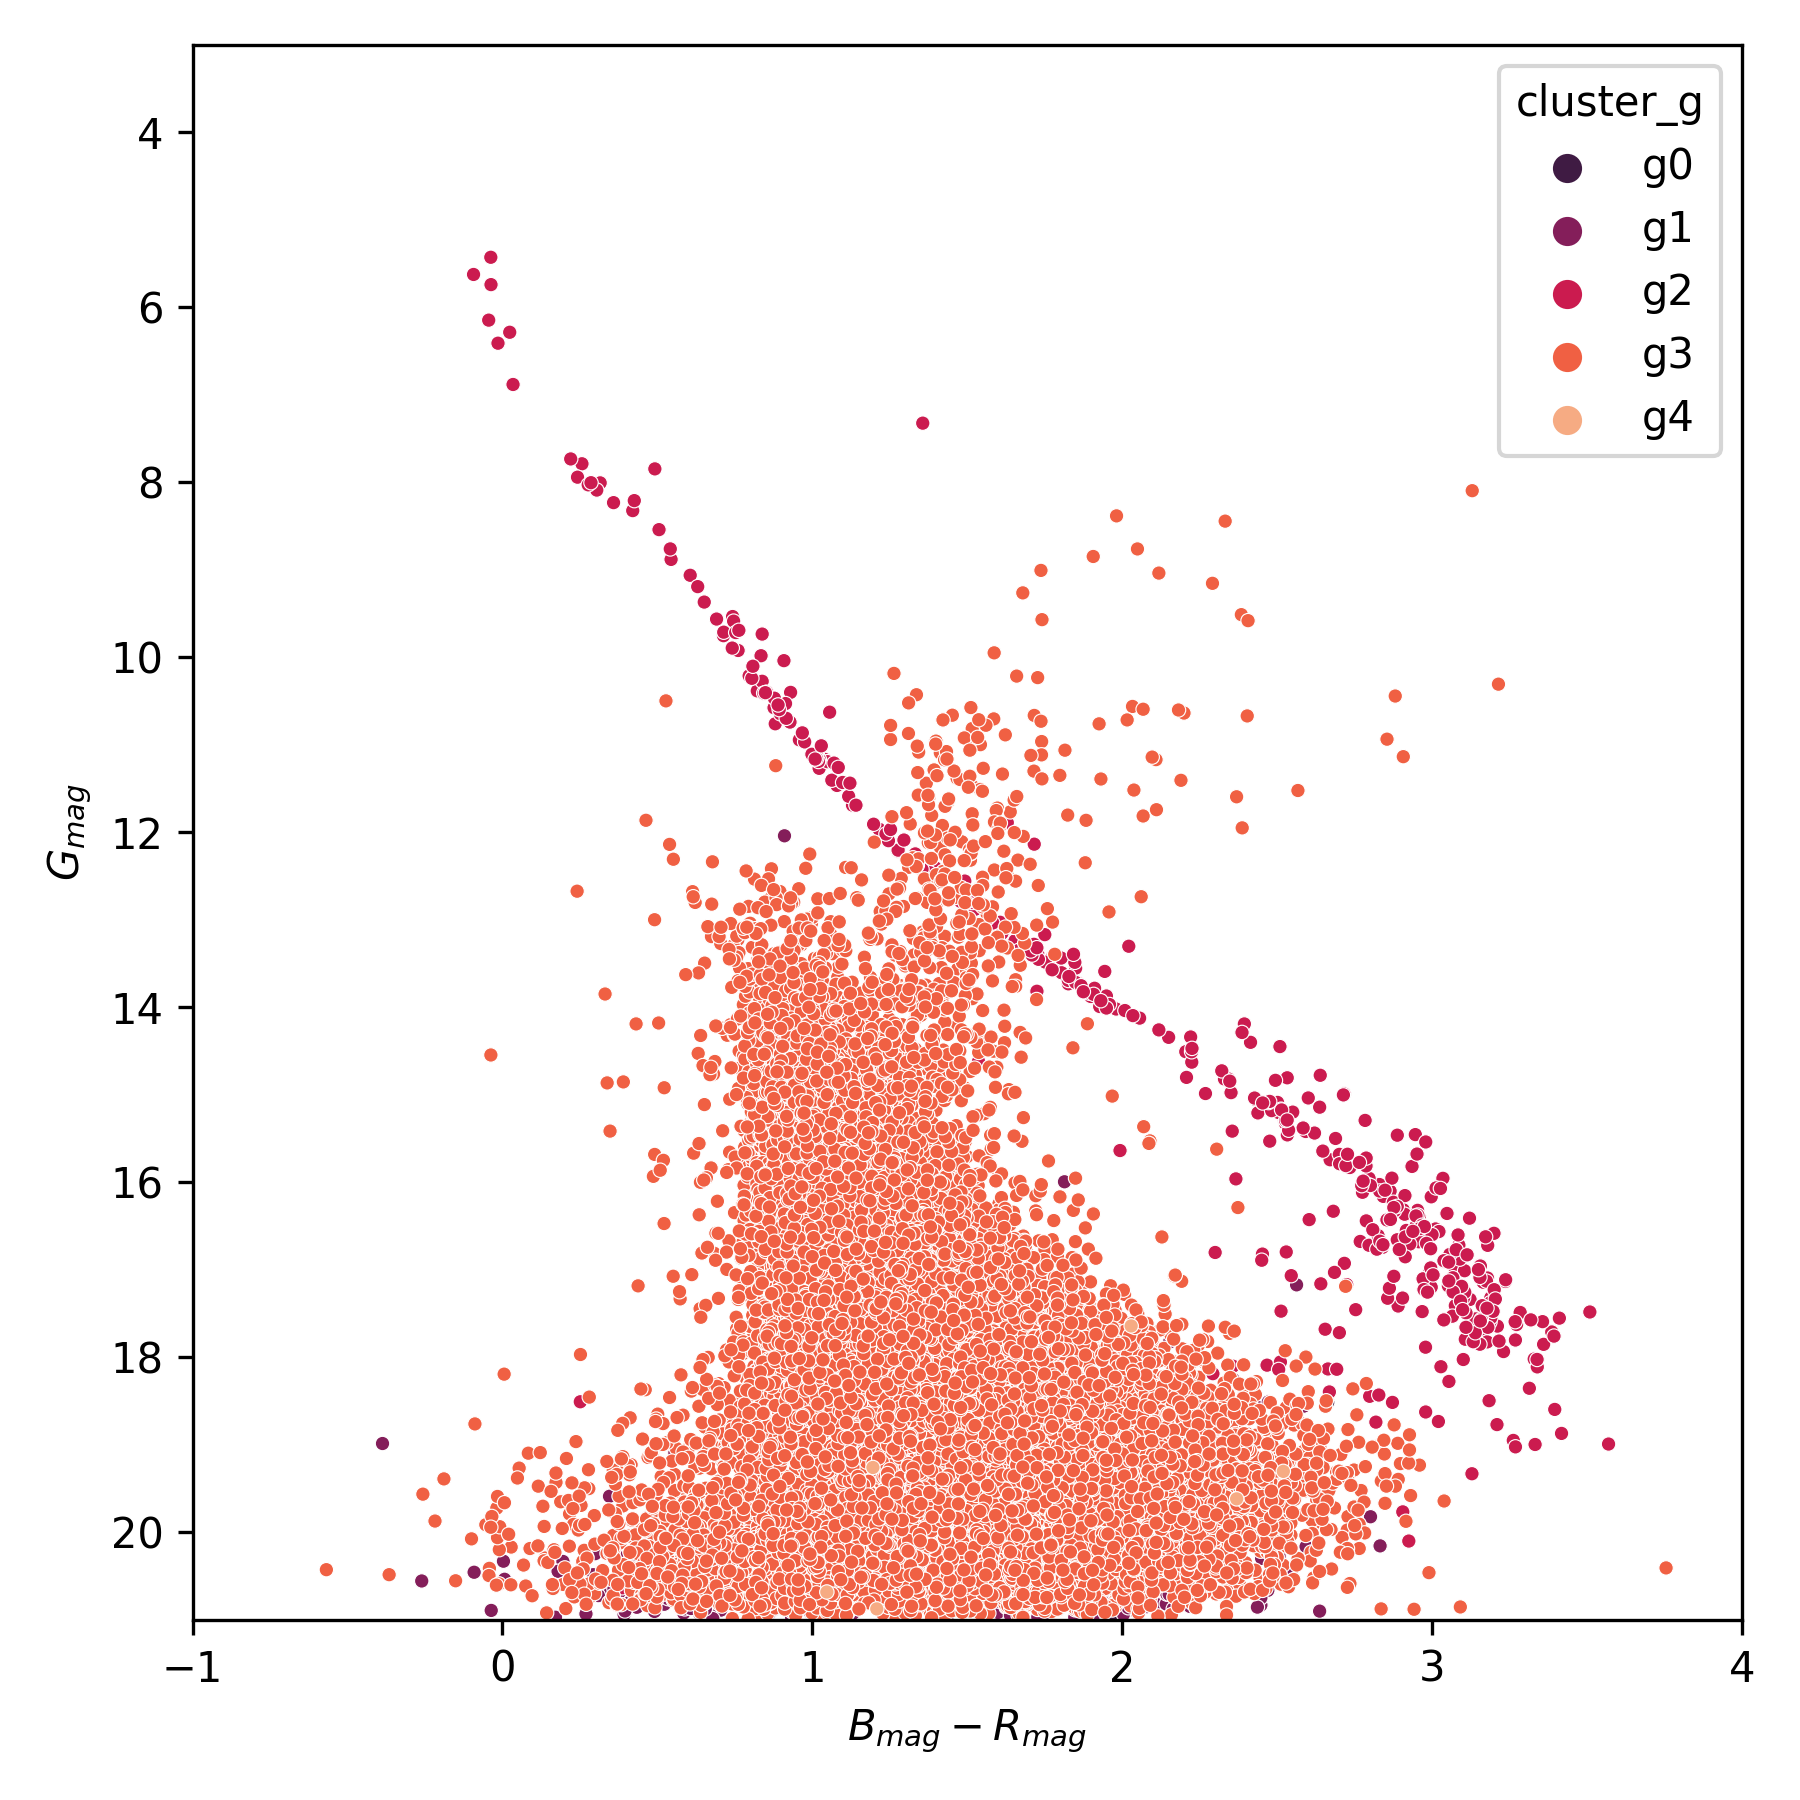
\includegraphics[width=\textwidth]{../figures/melotte_22/dec_hr_diagram_filtered_melotte_22.png}
      \caption{DEC (filt.)}
  \end{subfigure}
  \caption{Evolution of Melotte 22 characterization}
  \label{fig:melotte_22_characterization_evolution}
\end{figure*}

We have tested our model with the Melotte 25 dataset, which is one of the most difficult dataset
to characterize OC by its distribution and extension. In order to support the discussion presented
in Section~\ref{sec:deep_open_clustering}, we compared our model against a K-Means classification
algorithm. In addition, we perform a second execution only in our model where we filtered the
quantiles in the Melotte 22 dataset.

Our model was implemented in Python 3.8 using the Keras 2.2 framework and Jupyter
Notebooks~\cite{Kluyver2016jupyter}. All tests were run on an Apple Mac Pro Late 2013 with a
2.7GHz 12-Core Intel Xeon E5-2697v2, and 64GB RAM 1866MHz DDR3. For the GPU, we use a graphic
card AMD FirePro D700 with 6GB~\footnote{All resources developed for this project are available
at \href{https://github.com/cdalvaro/machine-learning-master-thesis}
{https://github.com/cdalvaro/machine-learning-master-thesis}}.

% More results are available at Appendix \ref{sec:appendix}.

Figure~\ref{fig:melotte_22_characterization_evolution} shows the evolution
of the characterization of Melotte 22. The first column corresponds to the
characterization obtained by applying K-Means alone to the dataset. The middle
column is the characterization made by the DEC model. And the column on the right
shows the characterization made by the DEC and having filtered the quantiles
lower than 0.10 and higher than 0.90. The top row shows the proper motion
configuration space while the bottom one shows the Hertzsprung–Russell diagrams.

%% Comparación con K-Means, DEC y DEC filter

Melotte 25 is located at 66.725 degrees in right ascension and 15.867
degrees in declination with a radius of 165 arcmin.
This region contains more than 400,000 stars.

Table~\ref{tab:results_melotte_25} shows a results summary for Melotte 25.

\begin{table}[!htbp]
  \begin{center}
    \resizebox{\columnwidth}{!}{
      \begin{tabular}{l|c|c|c|c}
        \textbf{Method} & \emph{\(\mu_{\alpha}\) \((mas \cdot yr^{-1})\)} & \emph{\(\mu_{\delta}\) \((mas \cdot yr^{-1})\)}
        & \emph{\( \varpi \) \((mas)\)} & \emph{\# stars} \\
        \hline
        \textbf{Simbad}\tablefootnote{Results have been taken from the SIMBAD astronomical database\cite{wenger2000simbad}}
        & 104.92 \( \pm \) 0.12 & -28.00 \( \pm \) 0.09 & 21.052 \( \pm \) 0.065 & - \\
        Clusterix & 106.796 \( \pm \) 6.229 & -24.870 \( \pm \) 5.417 & 21.210 \( \pm \) 1.115 & 109 \\
        K-Means & 79.936 \( \pm \) 3.7 & -45.362 \( \pm \) 3.8 & 20.901 \( \pm \) 0.31 & 374 \\
        DEC & 104.051 \( \pm \) 3.2 & -33.424 \( \pm \) 2.5 & 22.072 \( \pm \) 0.13 & 219 \\
        \textbf{DEC (filt.)} & 105.96 \( \pm \) 3.5 & -30.00 \( \pm \) 2.4 & 21.74 \( \pm \) 0.07 & 175 \\
      \end{tabular}
    }
    \caption{Melotte 25 results.}
    \label{tab:results_melotte_25}
  \end{center}
\end{table}

Parameters shown are proper motion in right ascension and declination, parallax
with their respective deviations and number of stars corresponding to the OC.

Figure~\ref{fig:result_melotte_25_dec} shows the groups found using the DEC model.
This model labels Melotte 25 as group \emph{g5}.

\begin{figure}[htbp]
  \centering
  \begin{subfigure}{\columnwidth}
    \centering
    \begin{subfigure}[t]{0.30\textwidth}
      \centering
      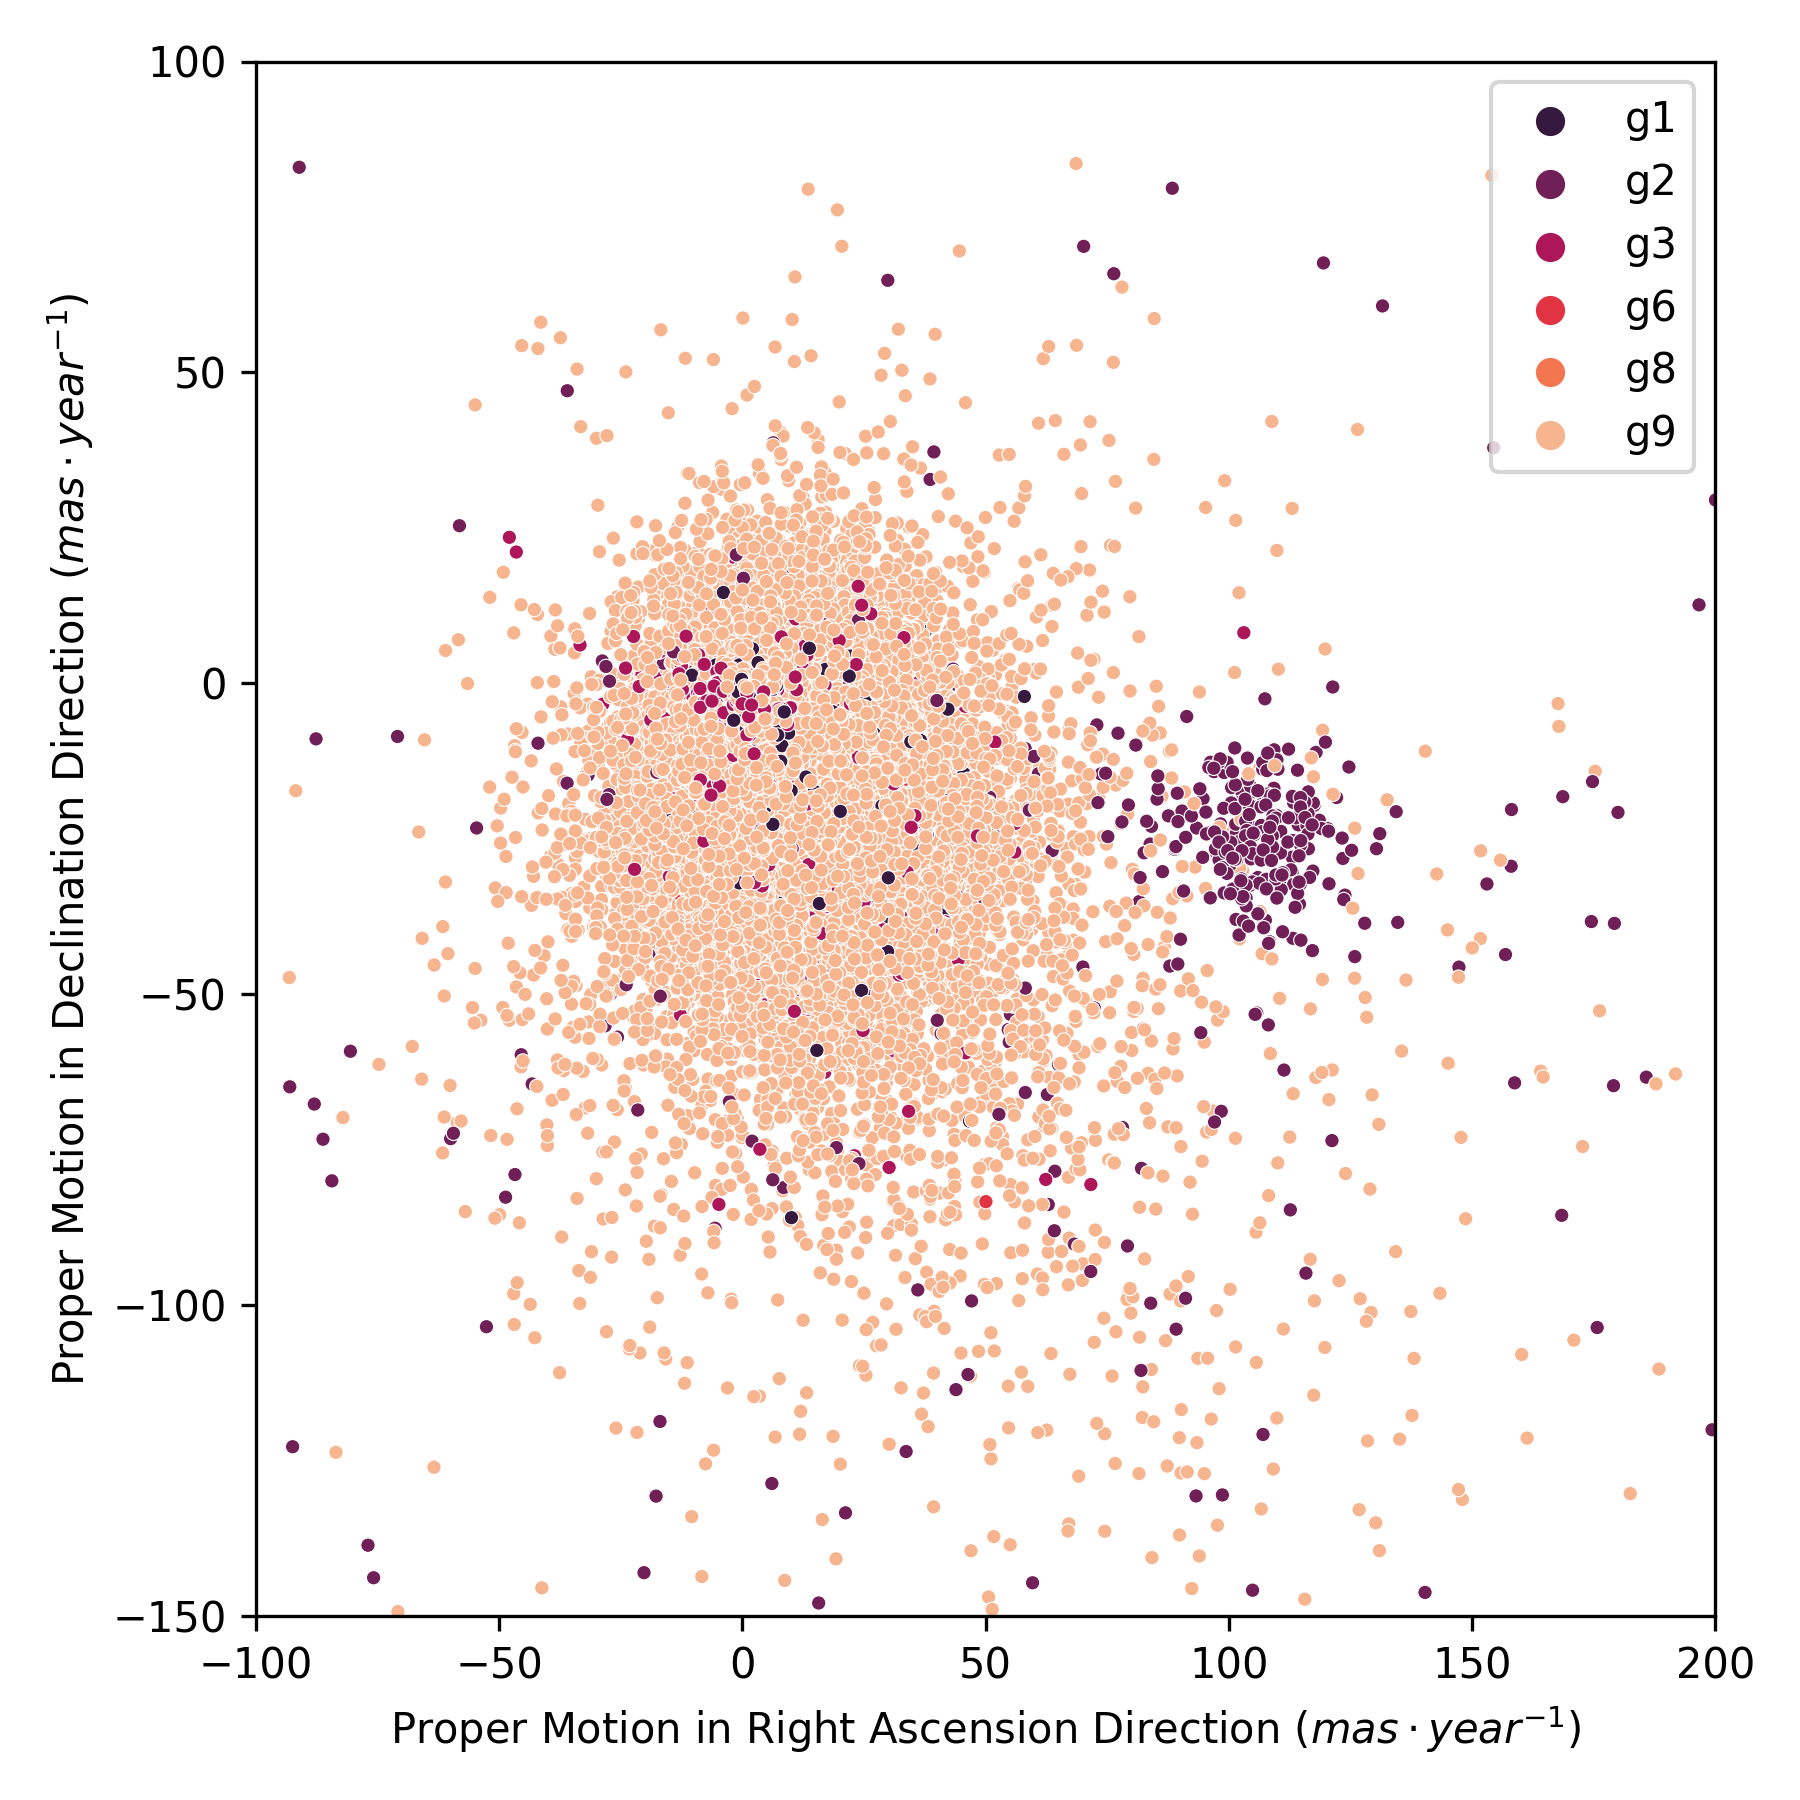
\includegraphics[width=\textwidth]{../figures/melotte_25/dec_pm_melotte_25.png}
    \end{subfigure}
    \hfill
    \begin{subfigure}[t]{0.30\textwidth}
      \centering
      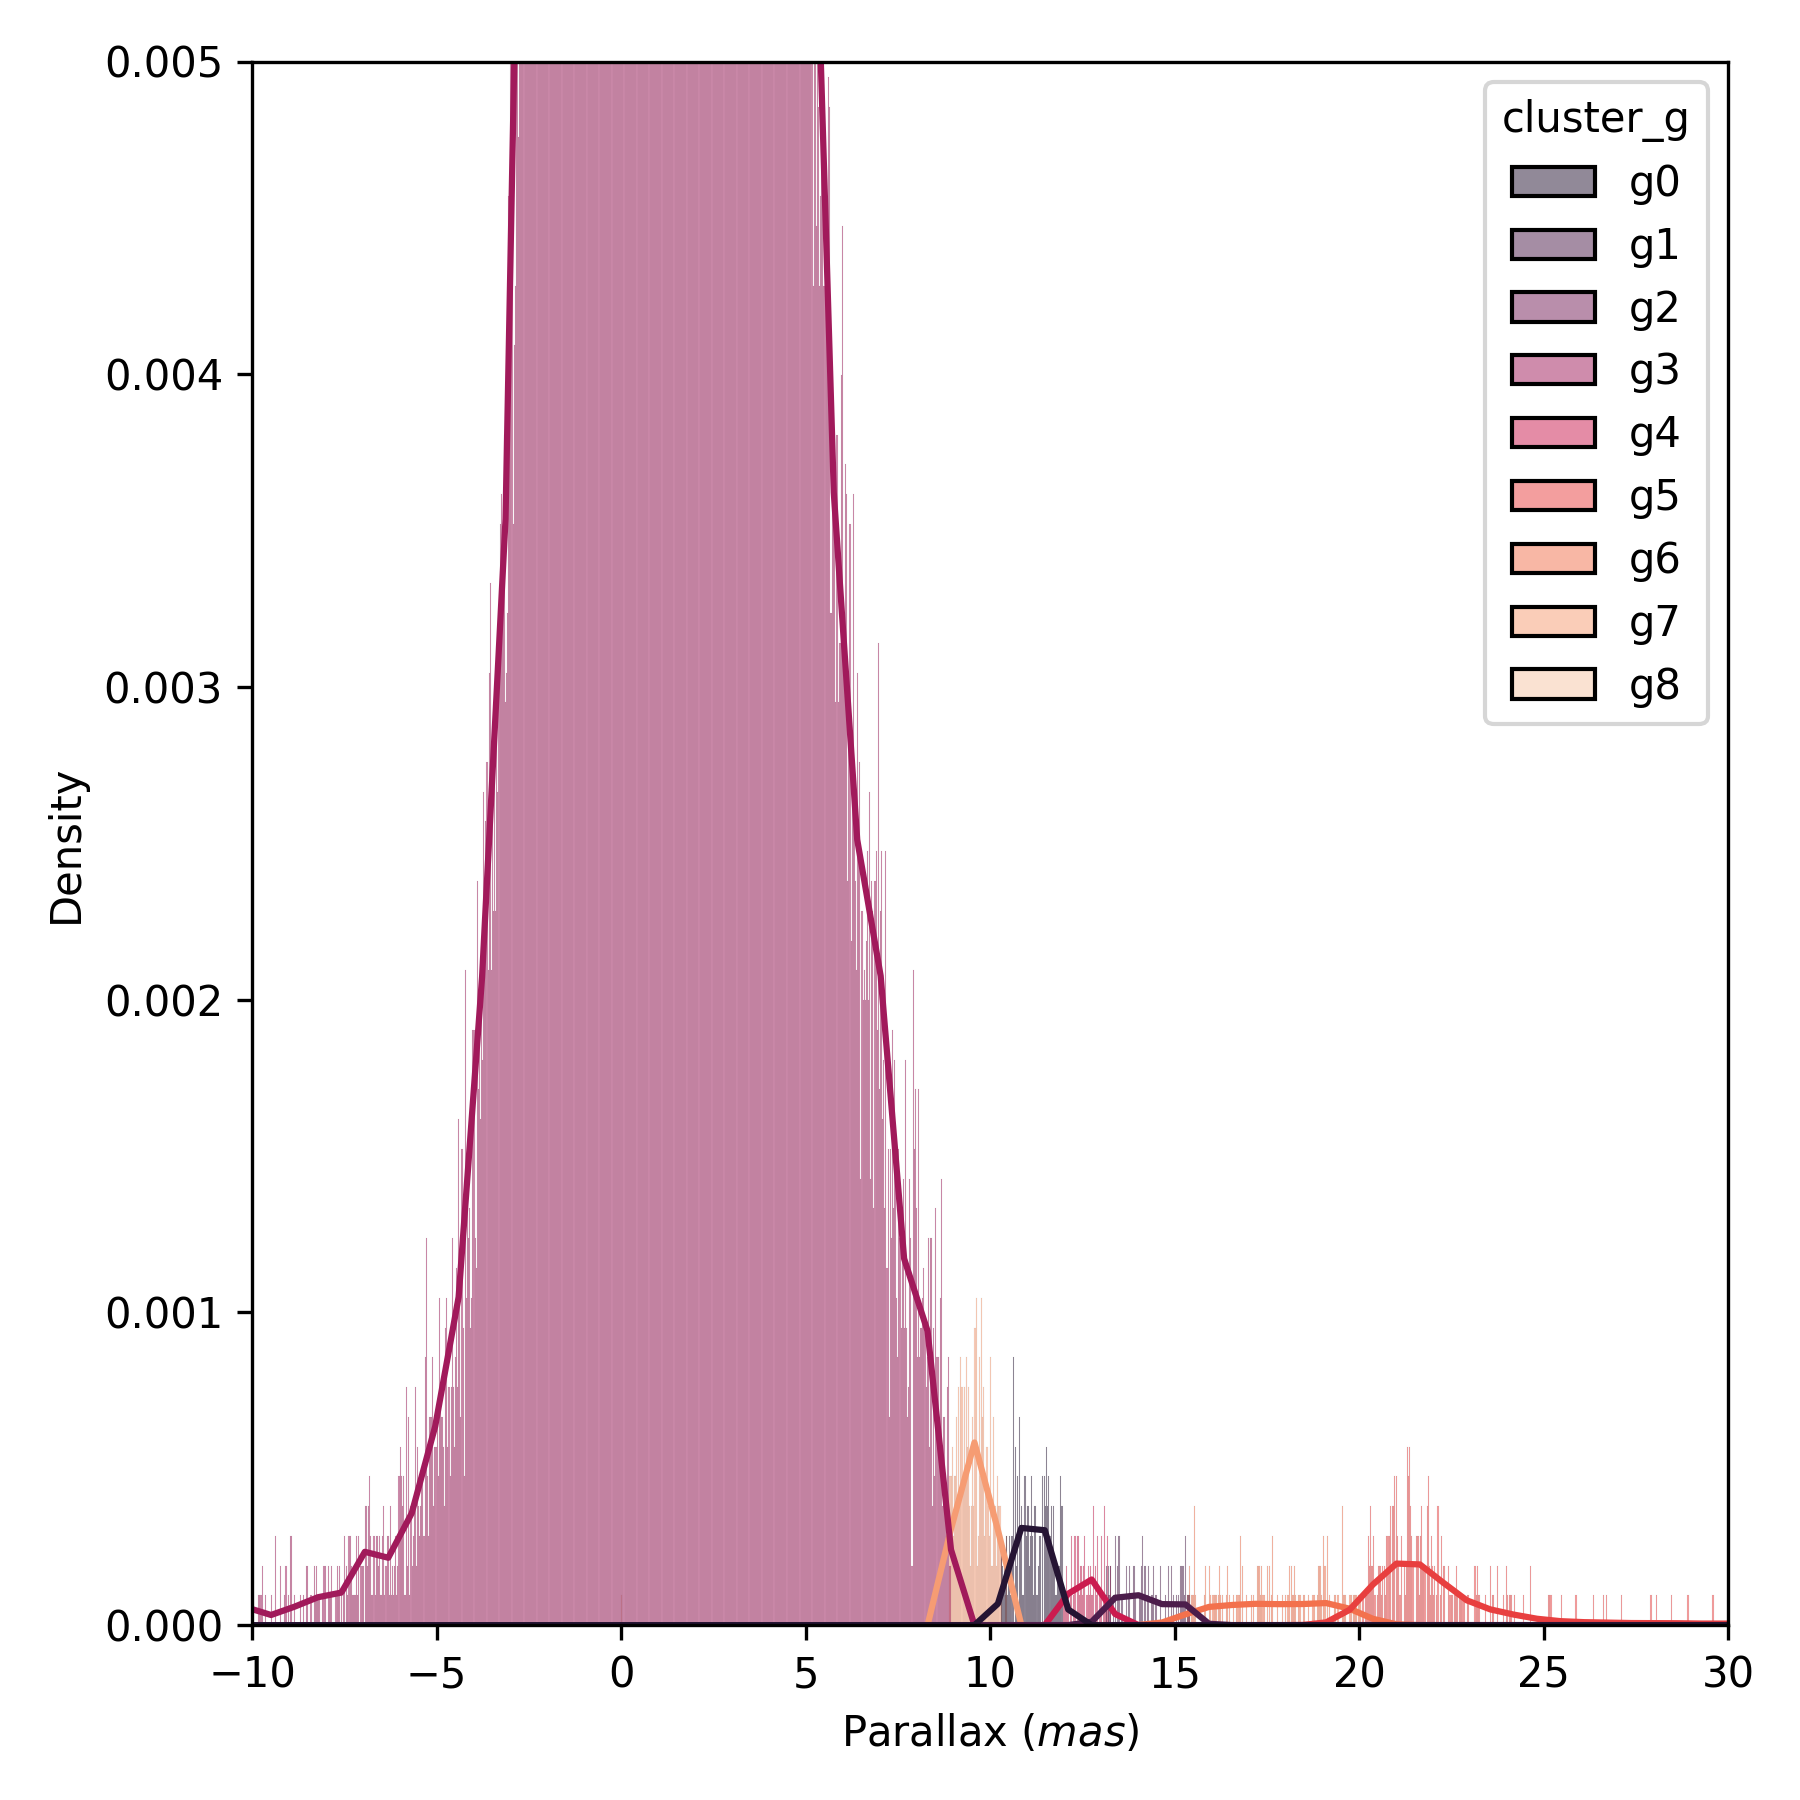
\includegraphics[width=\textwidth]{../figures/melotte_25/dec_parallax_melotte_25.png}
    \end{subfigure}
    \hfill
    \begin{subfigure}[t]{0.30\textwidth}
      \centering
      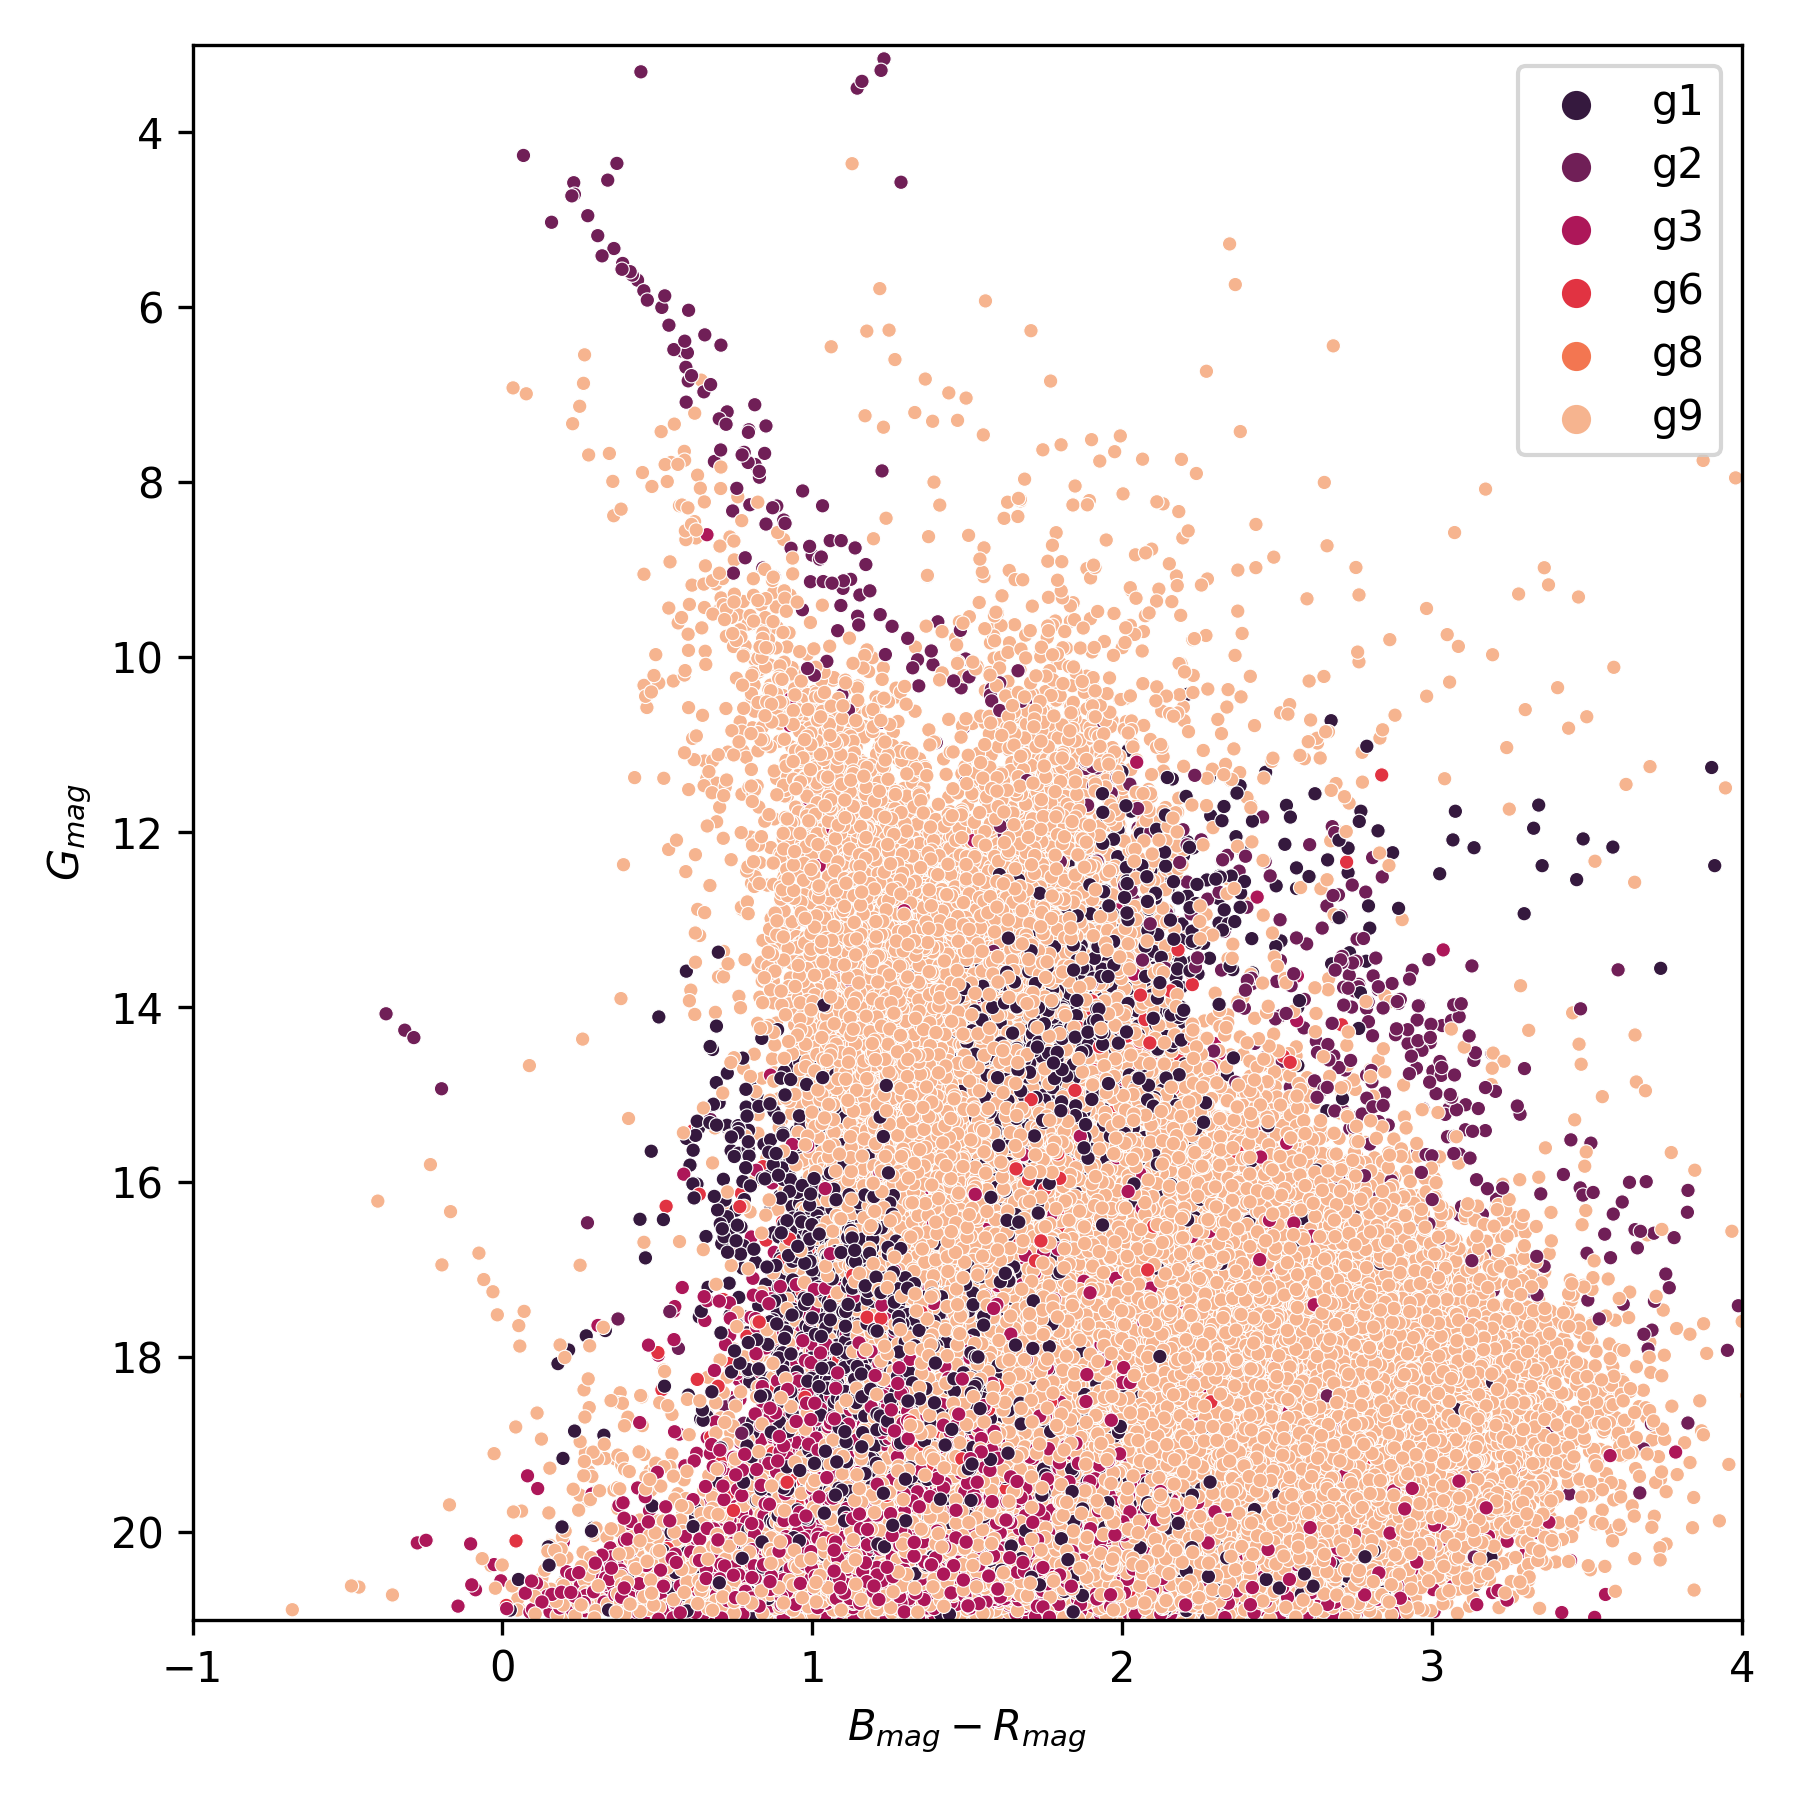
\includegraphics[width=\textwidth]{../figures/melotte_25/dec_hr_diagram_melotte_25.png}
    \end{subfigure}
  \end{subfigure}
  \caption{Melotte 25 characterization using the DEC model.
           From the left to the right: proper motion configuration
           space, parallax histogram and H-R diagram.}
  \label{fig:result_melotte_25_dec}
\end{figure}

Table~\ref{tab:hyperparameters_melotte_25} shows the hyperparameters
used for the characterization.

\begin{table}[h]
  \begin{center}
    \begin{tabular}{l|c}
      \textbf{Hyperparameter} & \textbf{Value} \\
      \hline
      Number of Clusters & 9 \\
      Clustering Layer & \(\left[ 50, 50, 40 \right]\) \\
      Kernel Initializer Seed & 11 \\
      Quantil Threshold & 0.1 \\
    \end{tabular}
    \caption{Melotte 25 DEC hyperparameters.}
    \label{tab:hyperparameters_melotte_25}
  \end{center}
\end{table}

\section{Result discussions}

We have applied our proposed method to clusters with different typologies:

\begin{itemize}
  \item NGC 2516 (Ap.~\ref{sec:ngc2516}) has it proper motion center deviated from the origin but
        it is embedded inside a big cloud of stars with similar proper motions.
  \item NGC 2632 (Ap.~\ref{sec:ngc2632}), in addition to Melotte 22, ia s cluster whose proper motion center
        is not located at the origin and has a well separated parallax center.
  \item NGC 2682 (Ap.~\ref{sec:ngc2682}), on the other hand, has its parallax centered within the region's gaussian,
        which complicates its detection although its proper motion center is deviated from the origin.
  \item Melotte 22 (Ap.~\ref{sec:melotte22}), as well as Melotte 25, is a cluster closer to us than the other.
        That makes its membership stars to be more scattered than previous clusters which are more compact.
\end{itemize}

All these clusters have a wide variety of diameters, from 25 to 330 arcmin,
as well as the number of stars that belong to them. NGC 2682 has 3,000 stars
while Melotte 25 is located inside a region with more than 400,000 stars.
More information about the studied clusters is available in Table~\ref{tab:clusters_summary}.

\begin{table}[htbp]
  \begin{center}
    \resizebox{\columnwidth}{!}{
      \begin{tabular}{l|c|c|c|c}
        \textbf{OC} & \emph{\( \alpha \) J2000 \((degrees)\)} & \emph{\( \delta \) J2000 \((degrees)\)}
        & \emph{Radius \((arcmin)\)} & \emph{\# stars} \\
        \hline
        NGC 2516 & 119.517 & -60.753 & 15 & 12,869 \\
        NGC 2632 & 130.1 & 19.667 & 35 & 13,167 \\
        NGC 2682 & 132.825 & 11.8 & 12.5 & 2,839 \\
        Melotte 22 & 56.75 & 24.117 & 60 & 61,552 \\
        Melotte 25 & 66.725 & 15.867 & 165 & 433,996 \\
      \end{tabular}
    }
    \caption{Right ascension, declination, radius and number of stars of studied clusters.
             The number of stars corresponds to those stars contained within a cone of center
             \((\alpha, \delta)\) and radius the cluster's radius multiplied by a factor of 1.5.}
    \label{tab:clusters_summary}
  \end{center}
\end{table}

In all cases, the model has resolved properly the identity of the cluster
and has characterized the membership stars, giving compatible results
with the ones obtained with classic procedures and VO tools.

Compared with the mentioned tools, our model can be categorized as a
non-parameterized model since it does not depend on parameters referred
to the cluster itself but only hyperparameters such as the initial number
of clusters to be found, or the structure of the Clustering Layer used by DEC model.

The proposed method is also non-supervised since we do not need to tell the model
which stars belong to the cluster or assist it while its training stage.

Only at the end of the characterization, a fine tuning driven by the user,
can be applied in order to improve the selection by discarding those
stars which fall outside the given quantiles.

In any case, we do not make assumptions about the cluster profile,
something that we have to take into account when using VO tools.
This is another evidence that our model is non-parameterized.

\section{Conclusions}

From the results shown in Section~\ref{sec:results}, we can say that, in general,
our model works fine identifying and characterizing open clusters.
So we have succeeded building a model non-parameterized and non-supervised
for open cluster characterization. However, some improvements should be done
in order to improve its accuracy and precision.

Another achievement is that we have developed a model that does not require
complex hardware. Instead, it can be run on workstations with a common GPU,
making it accessible to be implemented in many research centers.

We have built a non-parameterized model since the user is not required to provide
any information about the cluster profile or its properties.
Nevertheless some tweaks can be done regarding the cluster, like changing the initial
number of clusters or modifying the clustering layer structure in order to improve
the final characterization.

Another key point in our model is the initializer kernel.
This kernel prepares data before passing it to the ANN
and the results may vary significantly depending on this kernel.
This is something to avoid, so an improvement to solve this issue is necessary
in order to have a reliable model which does not depend on the dataset order.

Despite that, comparing our method with Clusterix, we can still say that the
number of parameters (or hyperparameters) in our model is smaller and that
we do not need previous knowledge about the studied cluster.
That makes easier to test different configurations and automate the process.

Furthermore, our model is able to deal with large and open regions. As an example,
it has succeeded characterizing Melotte 25 (Hiades) OC. Also, the relative proximity
of this cluster, 45 parsec, makes it difficult to characterize. Clusterix fails
characterizing this cluster. In this case, our method proposes at least two more
non-catalogued clusters. The analysis of these new clusters brings out an interesting
stellar dynamics in the studied region. It could mean that there was a recent
interaction among different molecular clouds.

For all this, we consider that the presented method is good enough to be included
in the Virtual Observatory toolset. Only a few tweaks must be done in order to make
our model compatible with other tools of the VO.

\subsection{Future work}

One open point to do from now is testing the model with a wider range of clusters.
In general we could think of applying it to the whole VizieR catalogue.
That way we could have a better idea about the current limitations of our model
and we could make some adjustments to improve it. We could determine with higher
accuracy the typologies that our model works well with, and which ones the model
does not resolve properly. Furthermore, we could stablish different sets of
hyperparameters regarding the typology of the cluster.

With our model, new uncatalogued clusters arise from the data apart of the main ones.
Hence, it is also interesting the individual study of these new clusters.

Another possible change in our model would be using DBSCAN instead of K-Means
as our initial clustering algorithm. Maybe this algorithm gives us a better starting
point for the DEC model which could improve the results.

Finally, we have used the Gaia DR2 database as our data source for this work,
but recently the DR3 dataset has been released.
Therefore, it is evident the interest on testing our model with this new data.

\appendix
\section{Appendix}
\label{sec:appendix}

\subsection{NGC 2516}
\label{sec:ngc2516}

\begin{table}[htbp]
  \begin{center}
    \resizebox{\columnwidth}{!}{
      \begin{tabular}{l|c|c|c|c}
        \textbf{Method} & \emph{\(\mu_{\alpha}\) \((mas \cdot yr^{-1})\)} & \emph{\(\mu_{\delta}\) \((mas \cdot yr^{-1})\)}
        & \emph{\( \varpi \) \((mas)\)} & \emph{\# stars} \\
        \hline
        \textbf{Simbad} & -4.6579 \( \pm \) 0.0075 & 11.1517 \( \pm \) 0.0075 & 2.4118 \( \pm \) 0.0006 & 1727 \\
        Clusterix & -4.652 \( \pm \) 0.523 & 11.203 \( \pm \) 0.454 & 2.409 \( \pm \) 0.127 & 638 \\
        K-Means & -4.344 \( \pm \) 0.14 & 9.507 \( \pm \) 0.19 & 2.268 \( \pm \) 0.01 & 1542 \\
        DEC & -4.426 \( \pm \) 0.17 & 9.952 \( \pm \) 0.20 & 2.436 \( \pm \) 0.01 & 1532 \\
        \textbf{DEC (filt.)} & -4.502 \( \pm \) 0.14 & 10.114 \( \pm \) 0.17 & 2.392 \( \pm \) 0.004 & 1072 \\
      \end{tabular}
    }
    \caption{NGC 2516 results.}
    \label{tab:app_results_ngc_2516}
  \end{center}
\end{table}

Table~\ref{tab:app_results_ngc_2516} shows a results summary for NGC 2516.
The top row of Figure~\ref{fig:app_result_ngc_2516_clusterix_kmeans} shows
the characterization using Clusterix+TOPCAT tools while the bottom row
shows eight clusters found by K-Means.

\begin{figure}[htbp]
  \centering
  \begin{subfigure}{\columnwidth}
    \centering
    \begin{subfigure}[t]{0.30\textwidth}
      \centering
      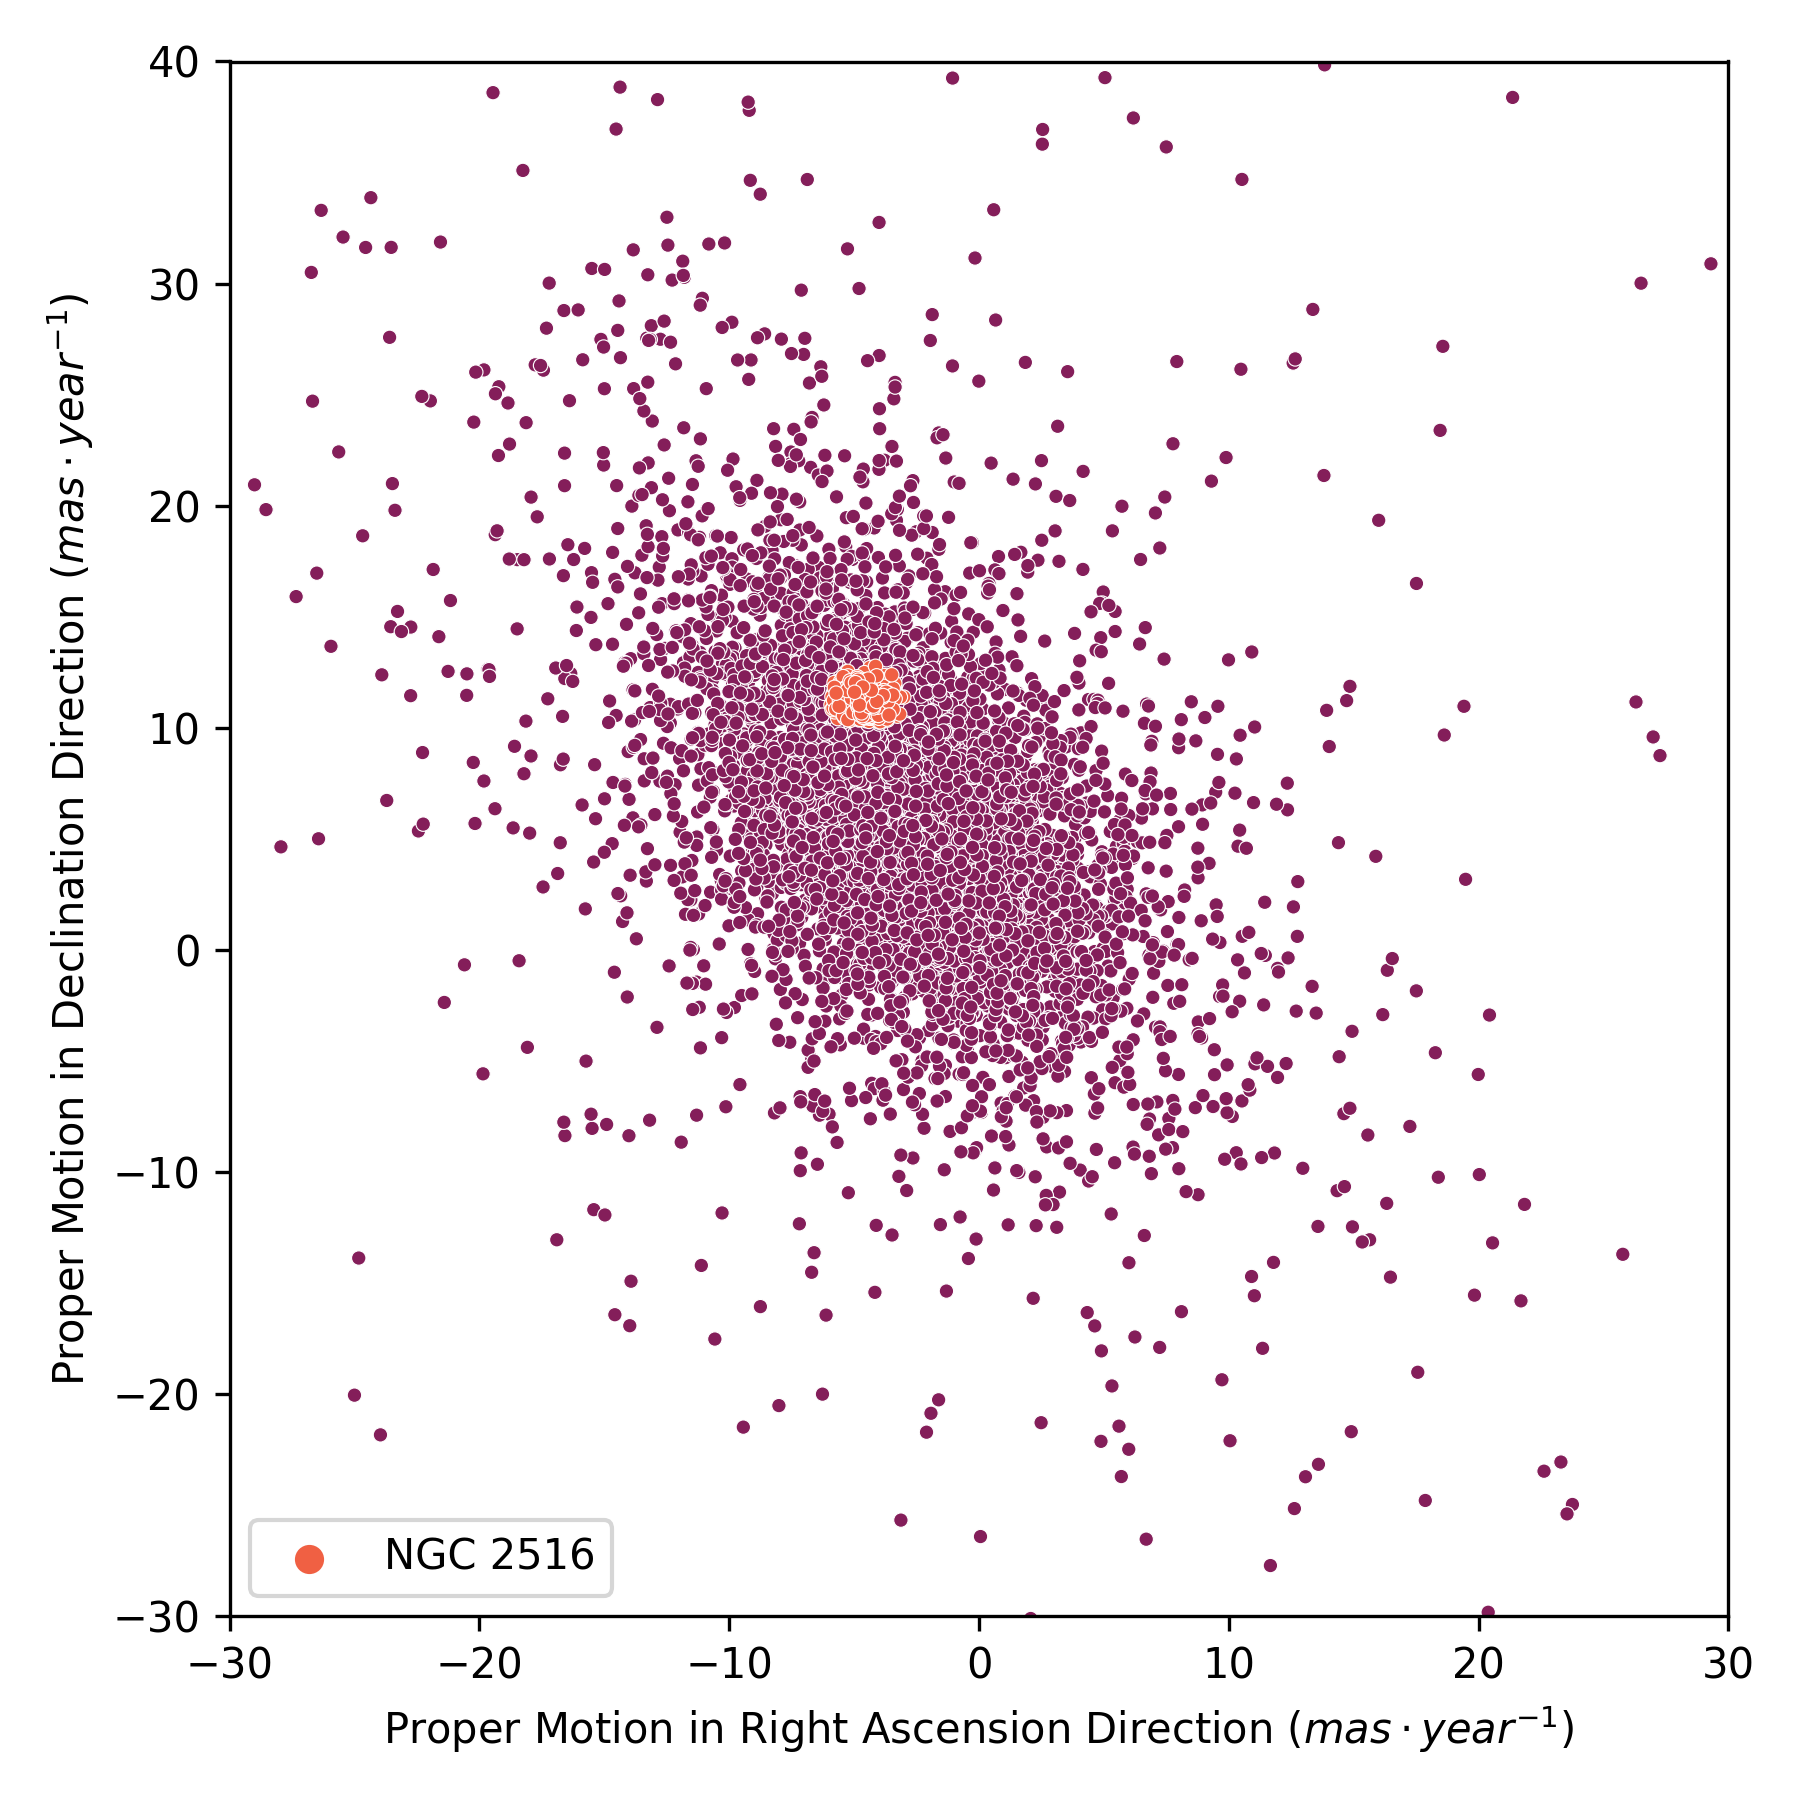
\includegraphics[width=\textwidth]{../figures/ngc_2516/pm_ngc_2516.png}
    \end{subfigure}
    \hfill
    \begin{subfigure}[t]{0.30\textwidth}
      \centering
      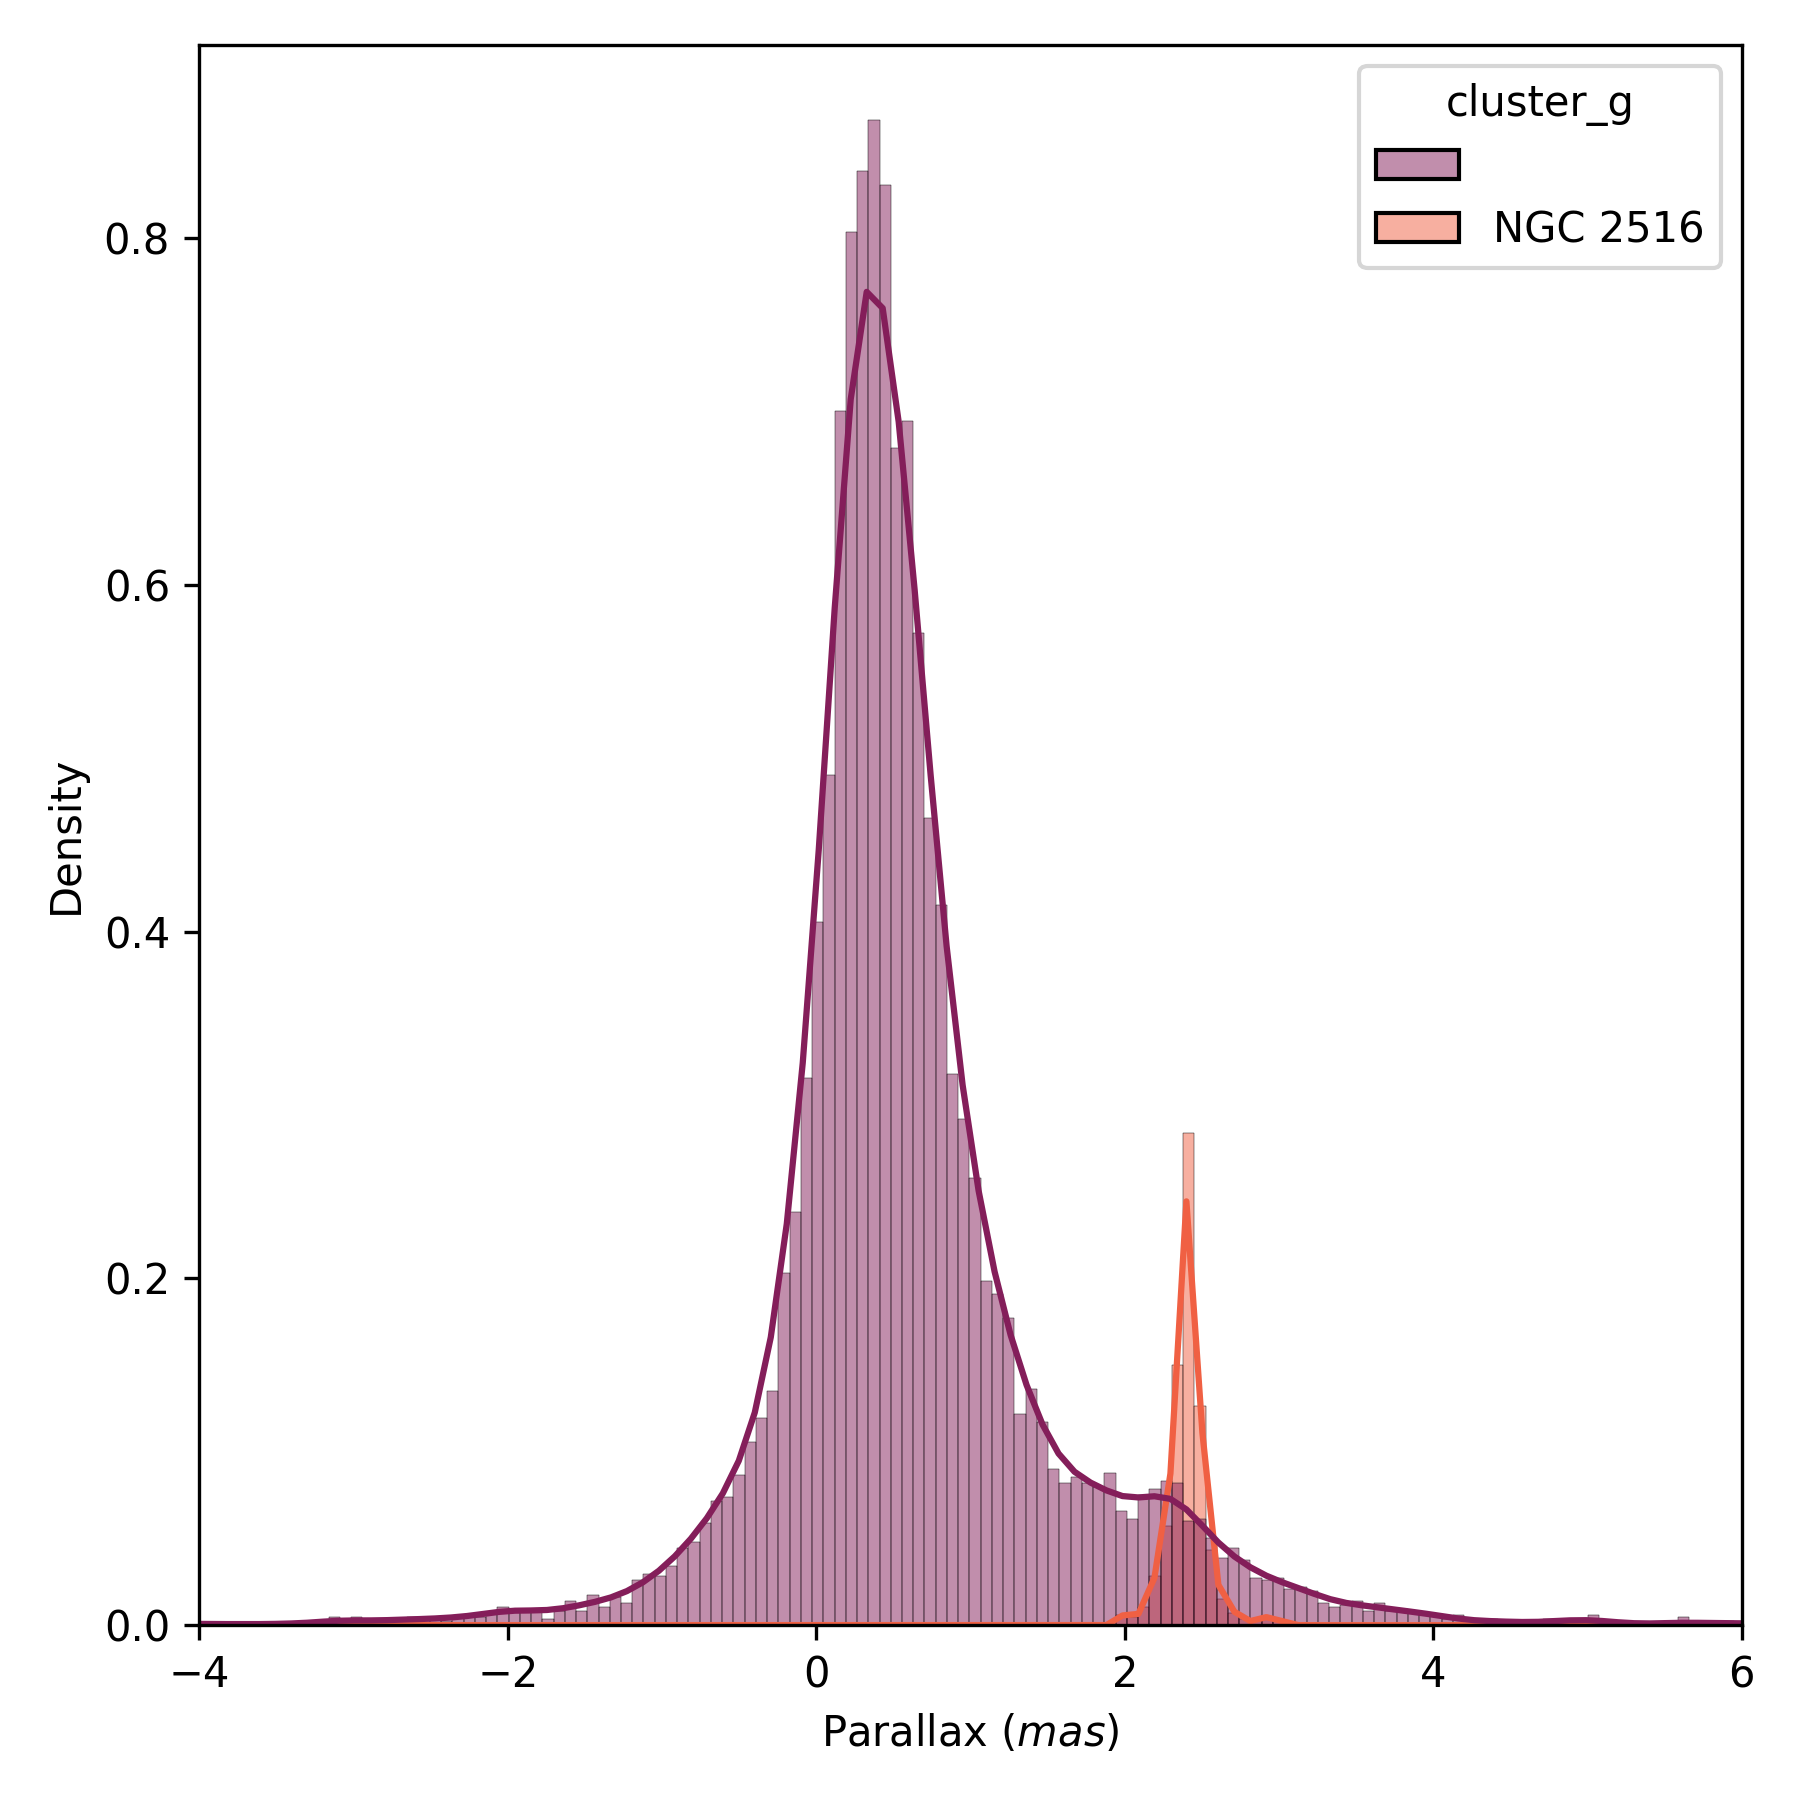
\includegraphics[width=\textwidth]{../figures/ngc_2516/parallax_ngc_2516.png}
    \end{subfigure}
    \hfill
    \begin{subfigure}[t]{0.30\textwidth}
      \centering
      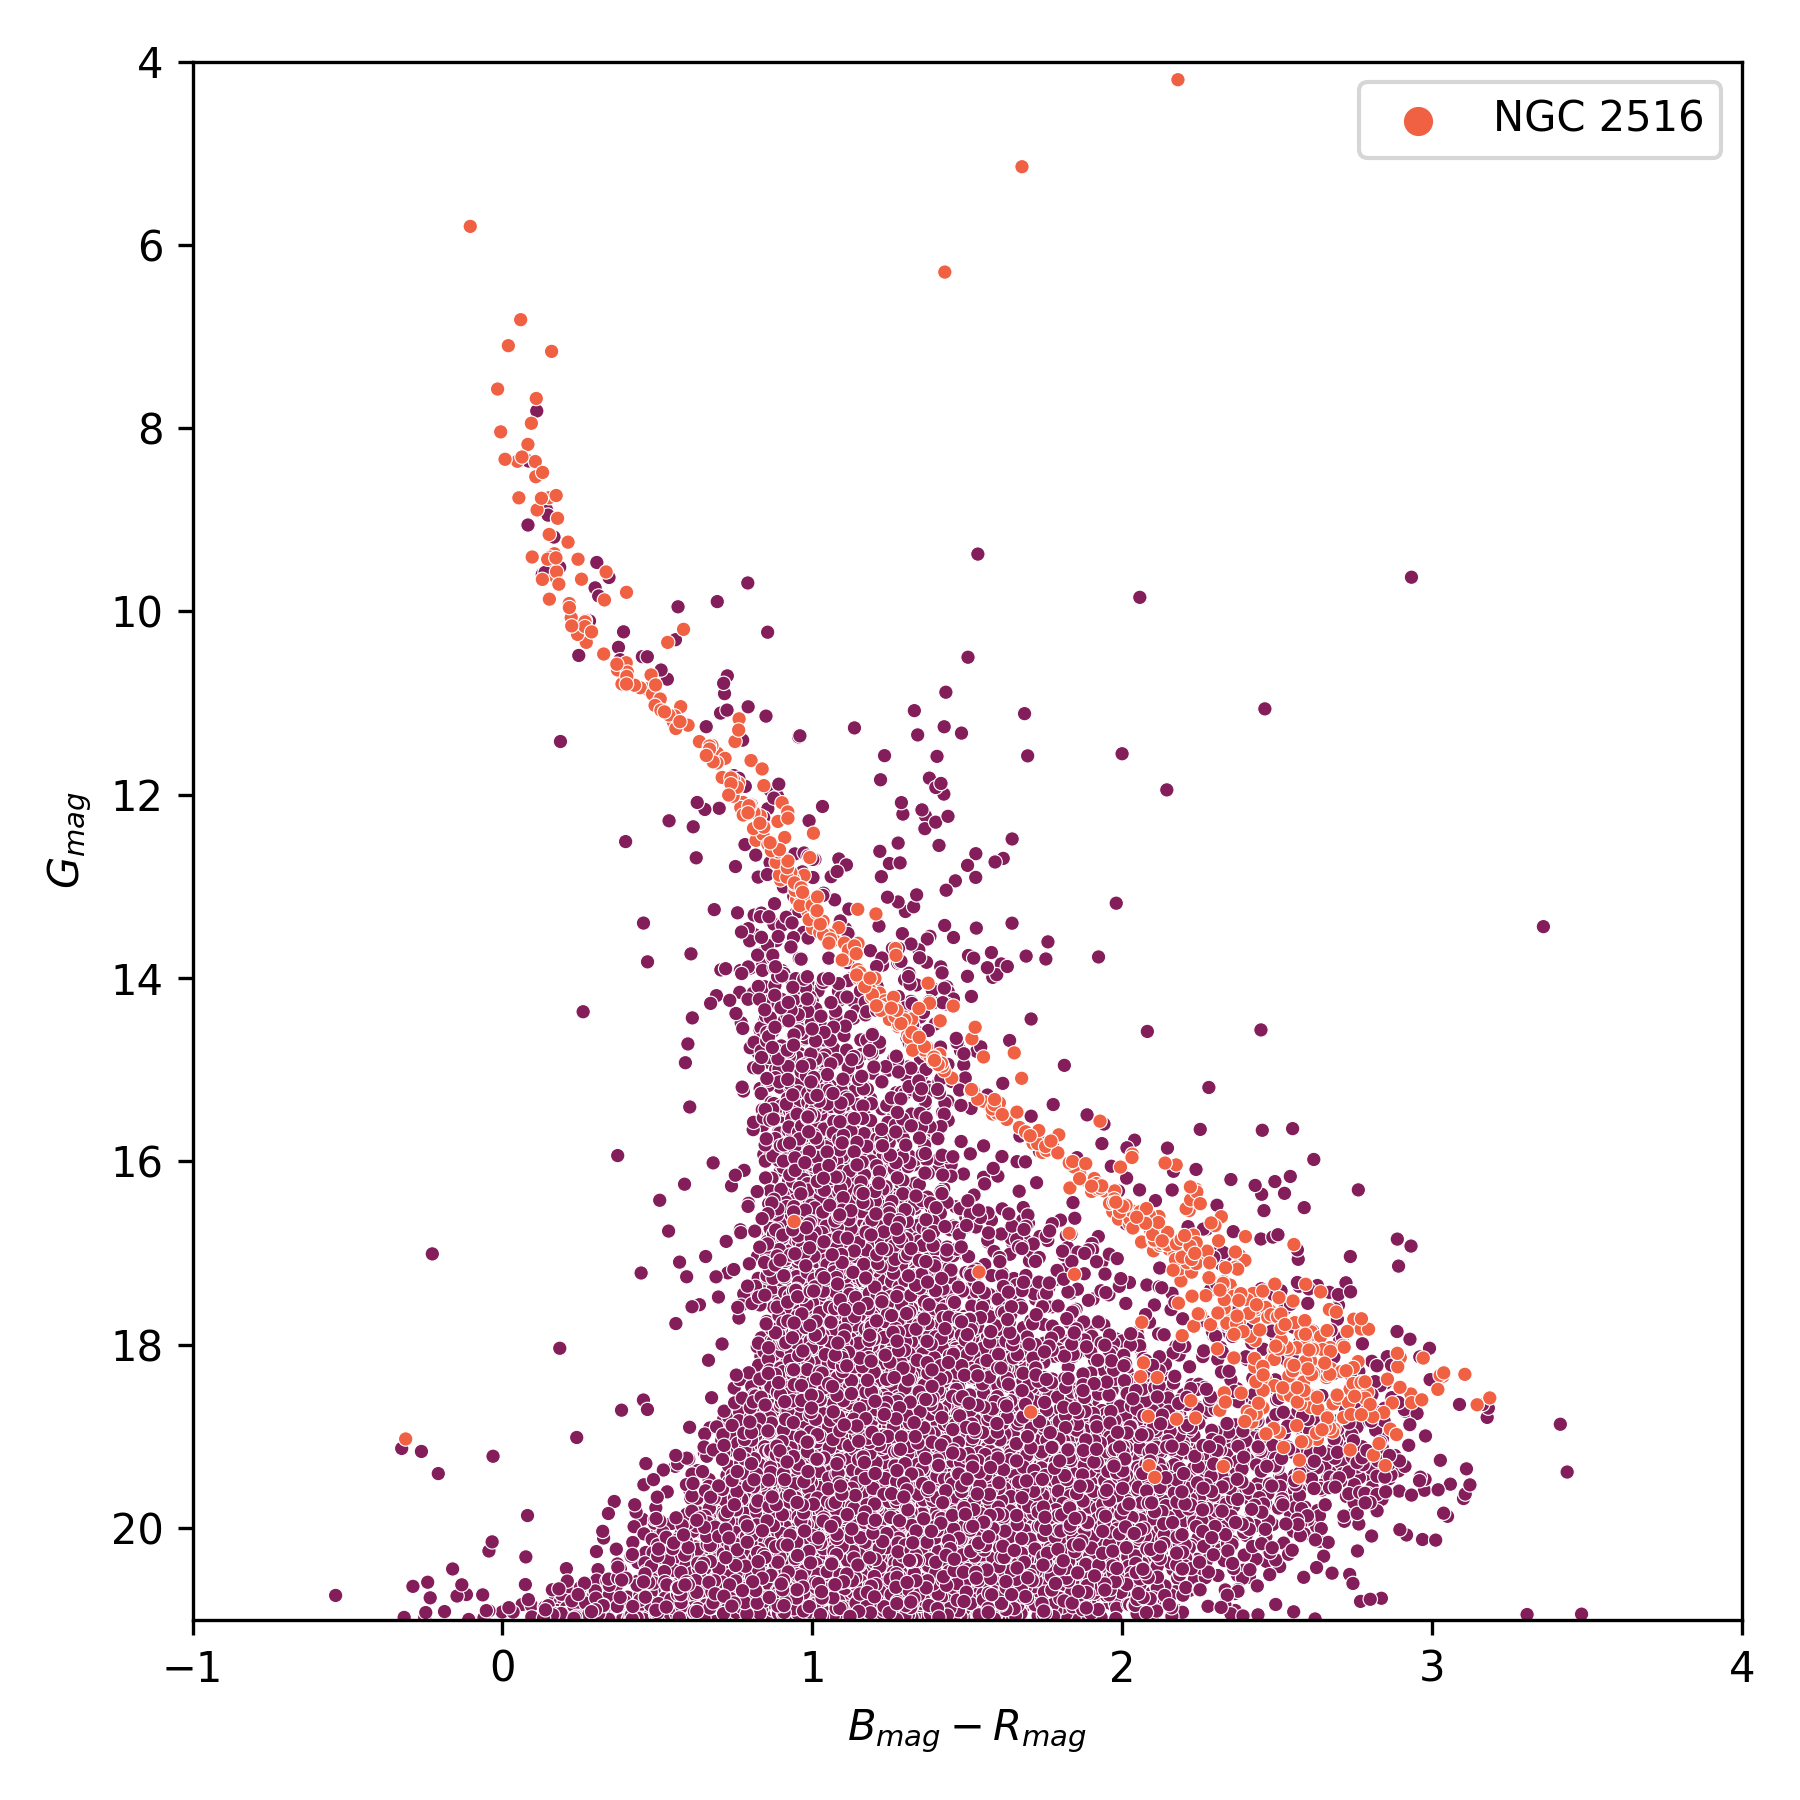
\includegraphics[width=\textwidth]{../figures/ngc_2516/hr_diagram_ngc_2516.png}
    \end{subfigure}
  \end{subfigure}
  \centering
  \begin{subfigure}{\columnwidth}
    \centering
    \begin{subfigure}[t]{0.30\textwidth}
      \centering
      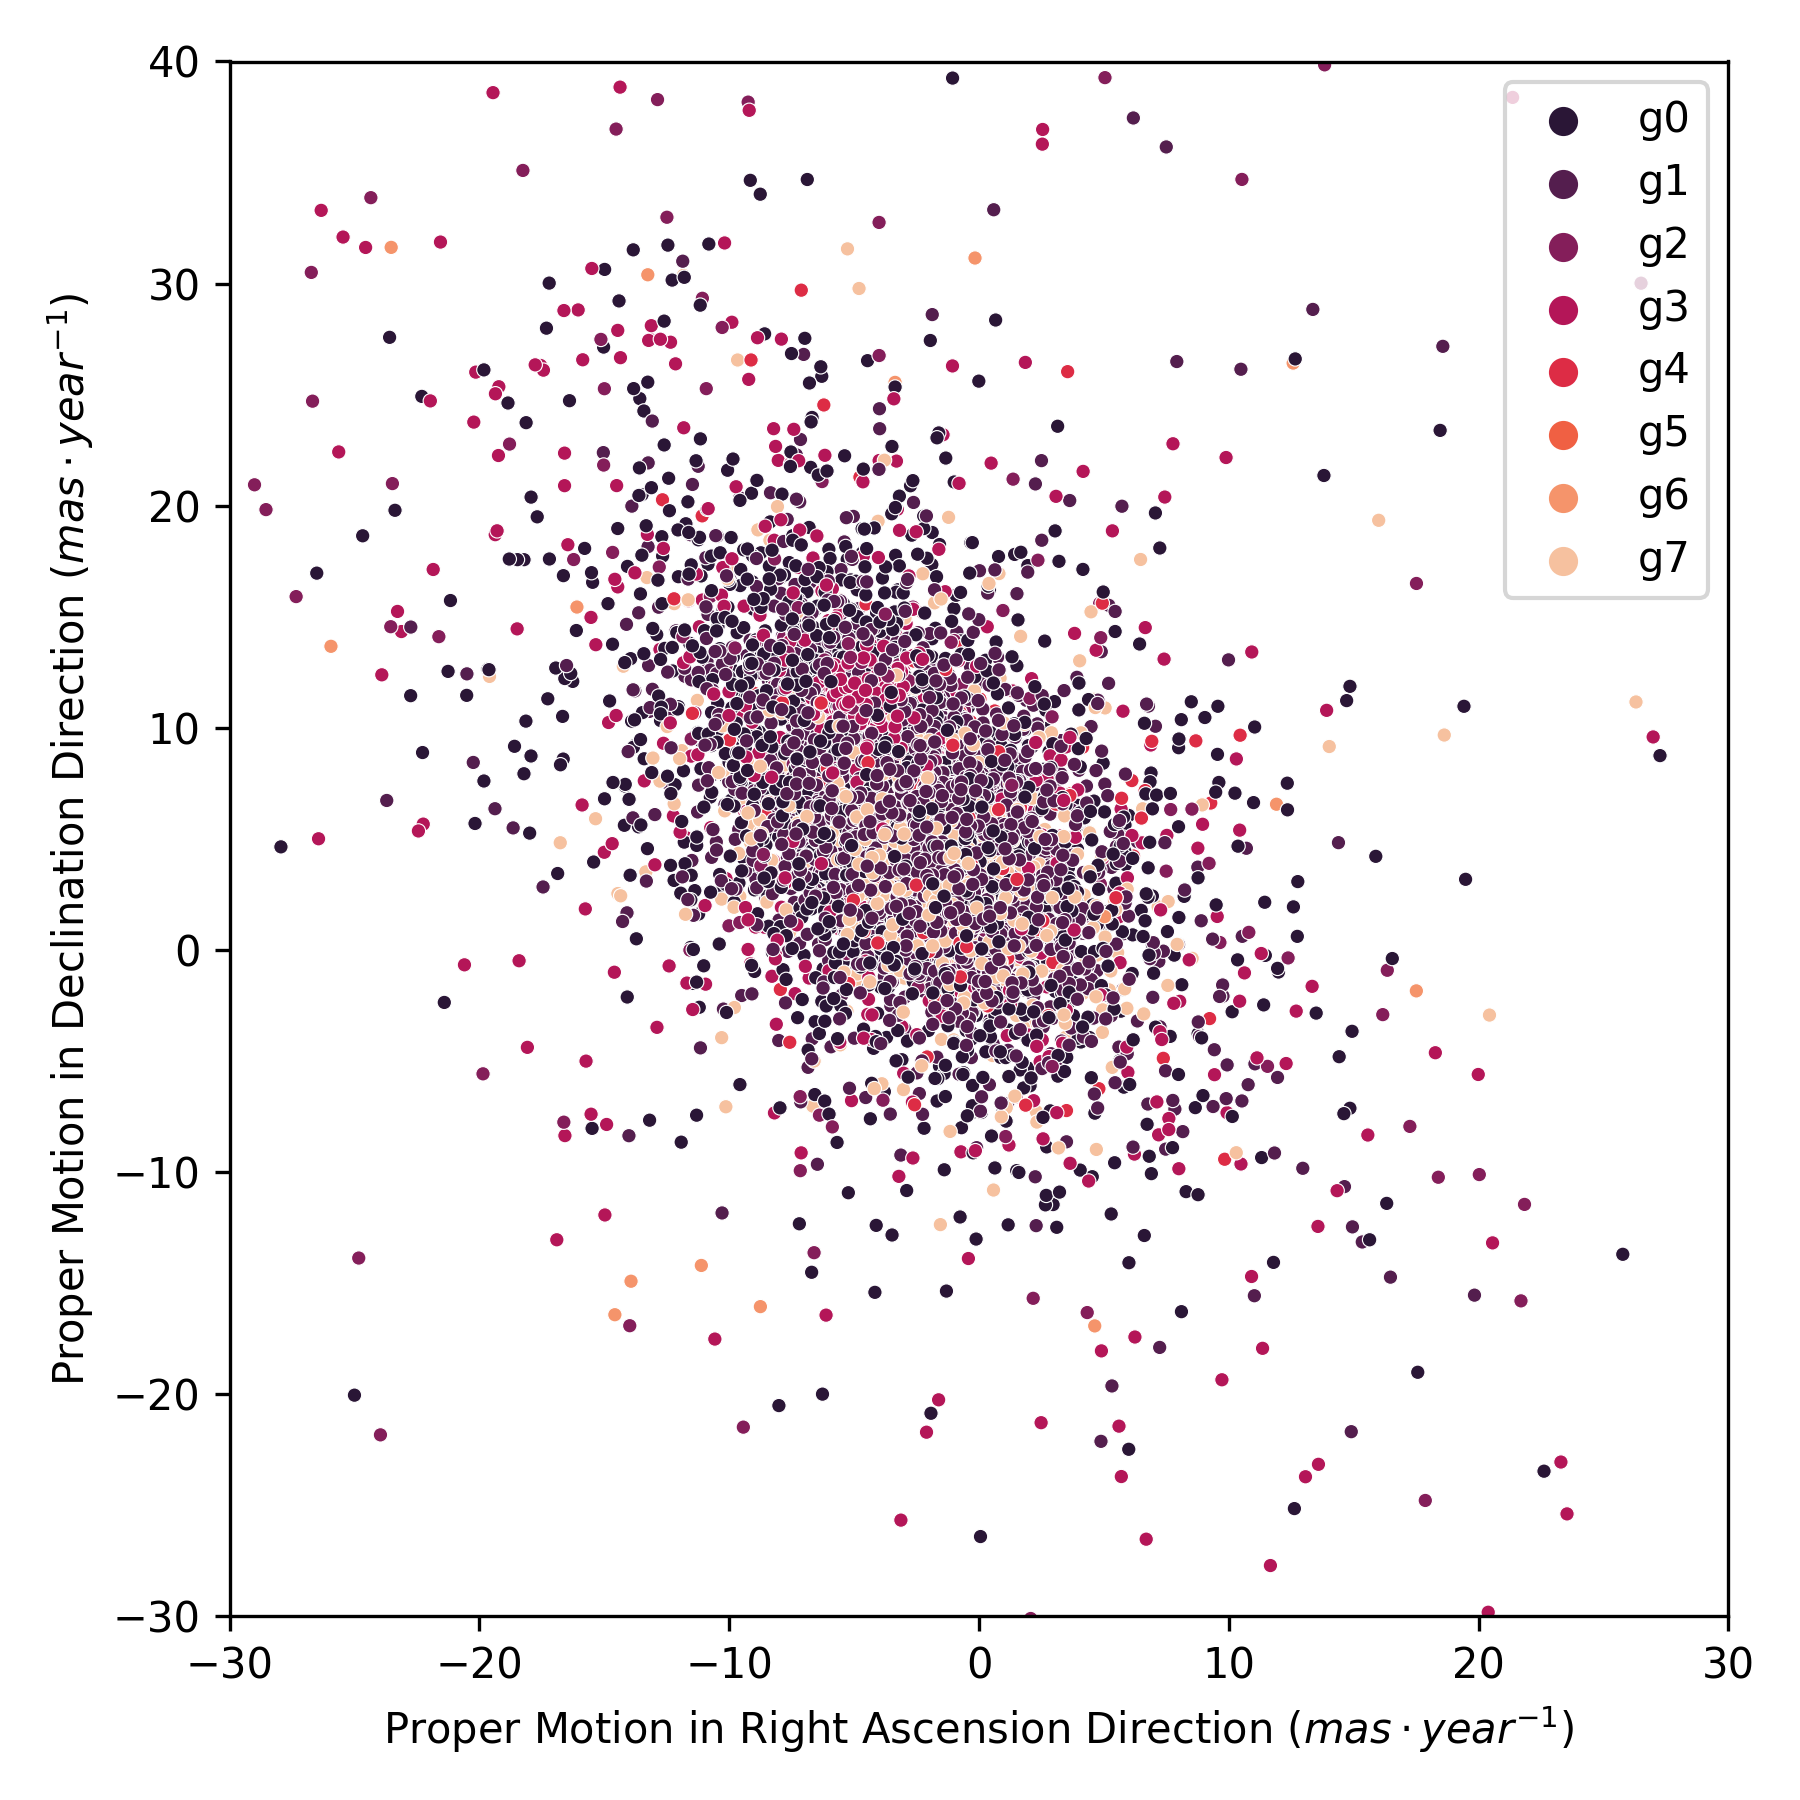
\includegraphics[width=\textwidth]{../figures/ngc_2516/kmeans_pm_ngc_2516.png}
    \end{subfigure}
    \hfill
    \begin{subfigure}[t]{0.30\textwidth}
      \centering
      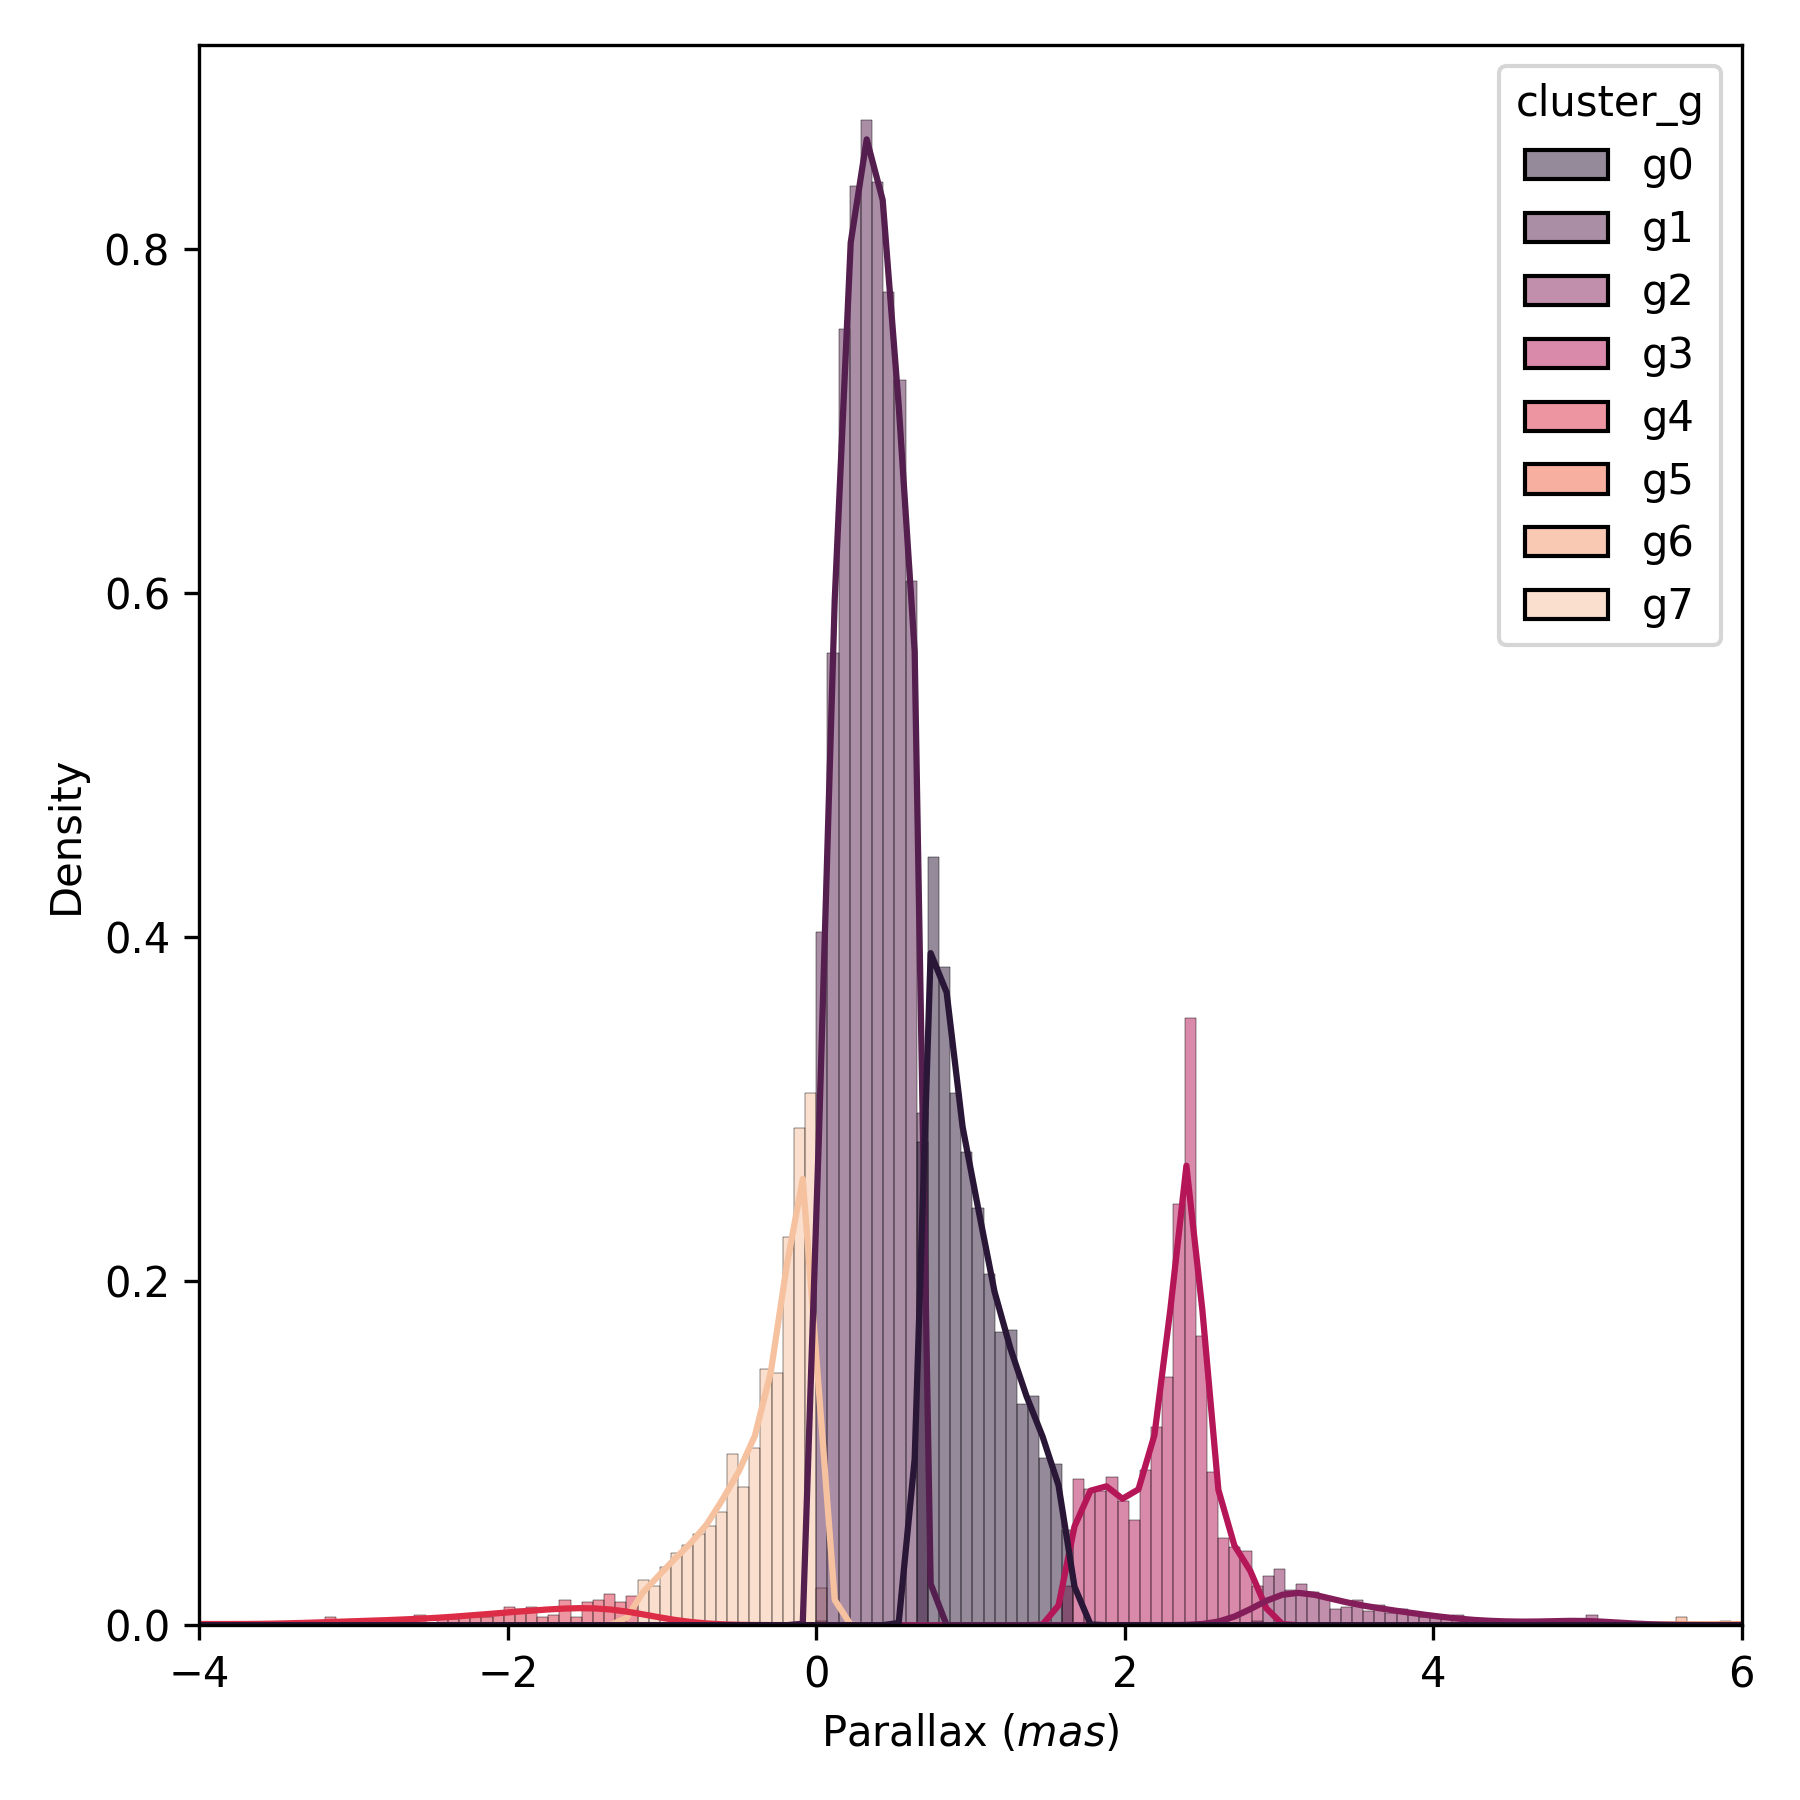
\includegraphics[width=\textwidth]{../figures/ngc_2516/kmeans_parallax_ngc_2516.png}
    \end{subfigure}
    \hfill
    \begin{subfigure}[t]{0.30\textwidth}
      \centering
      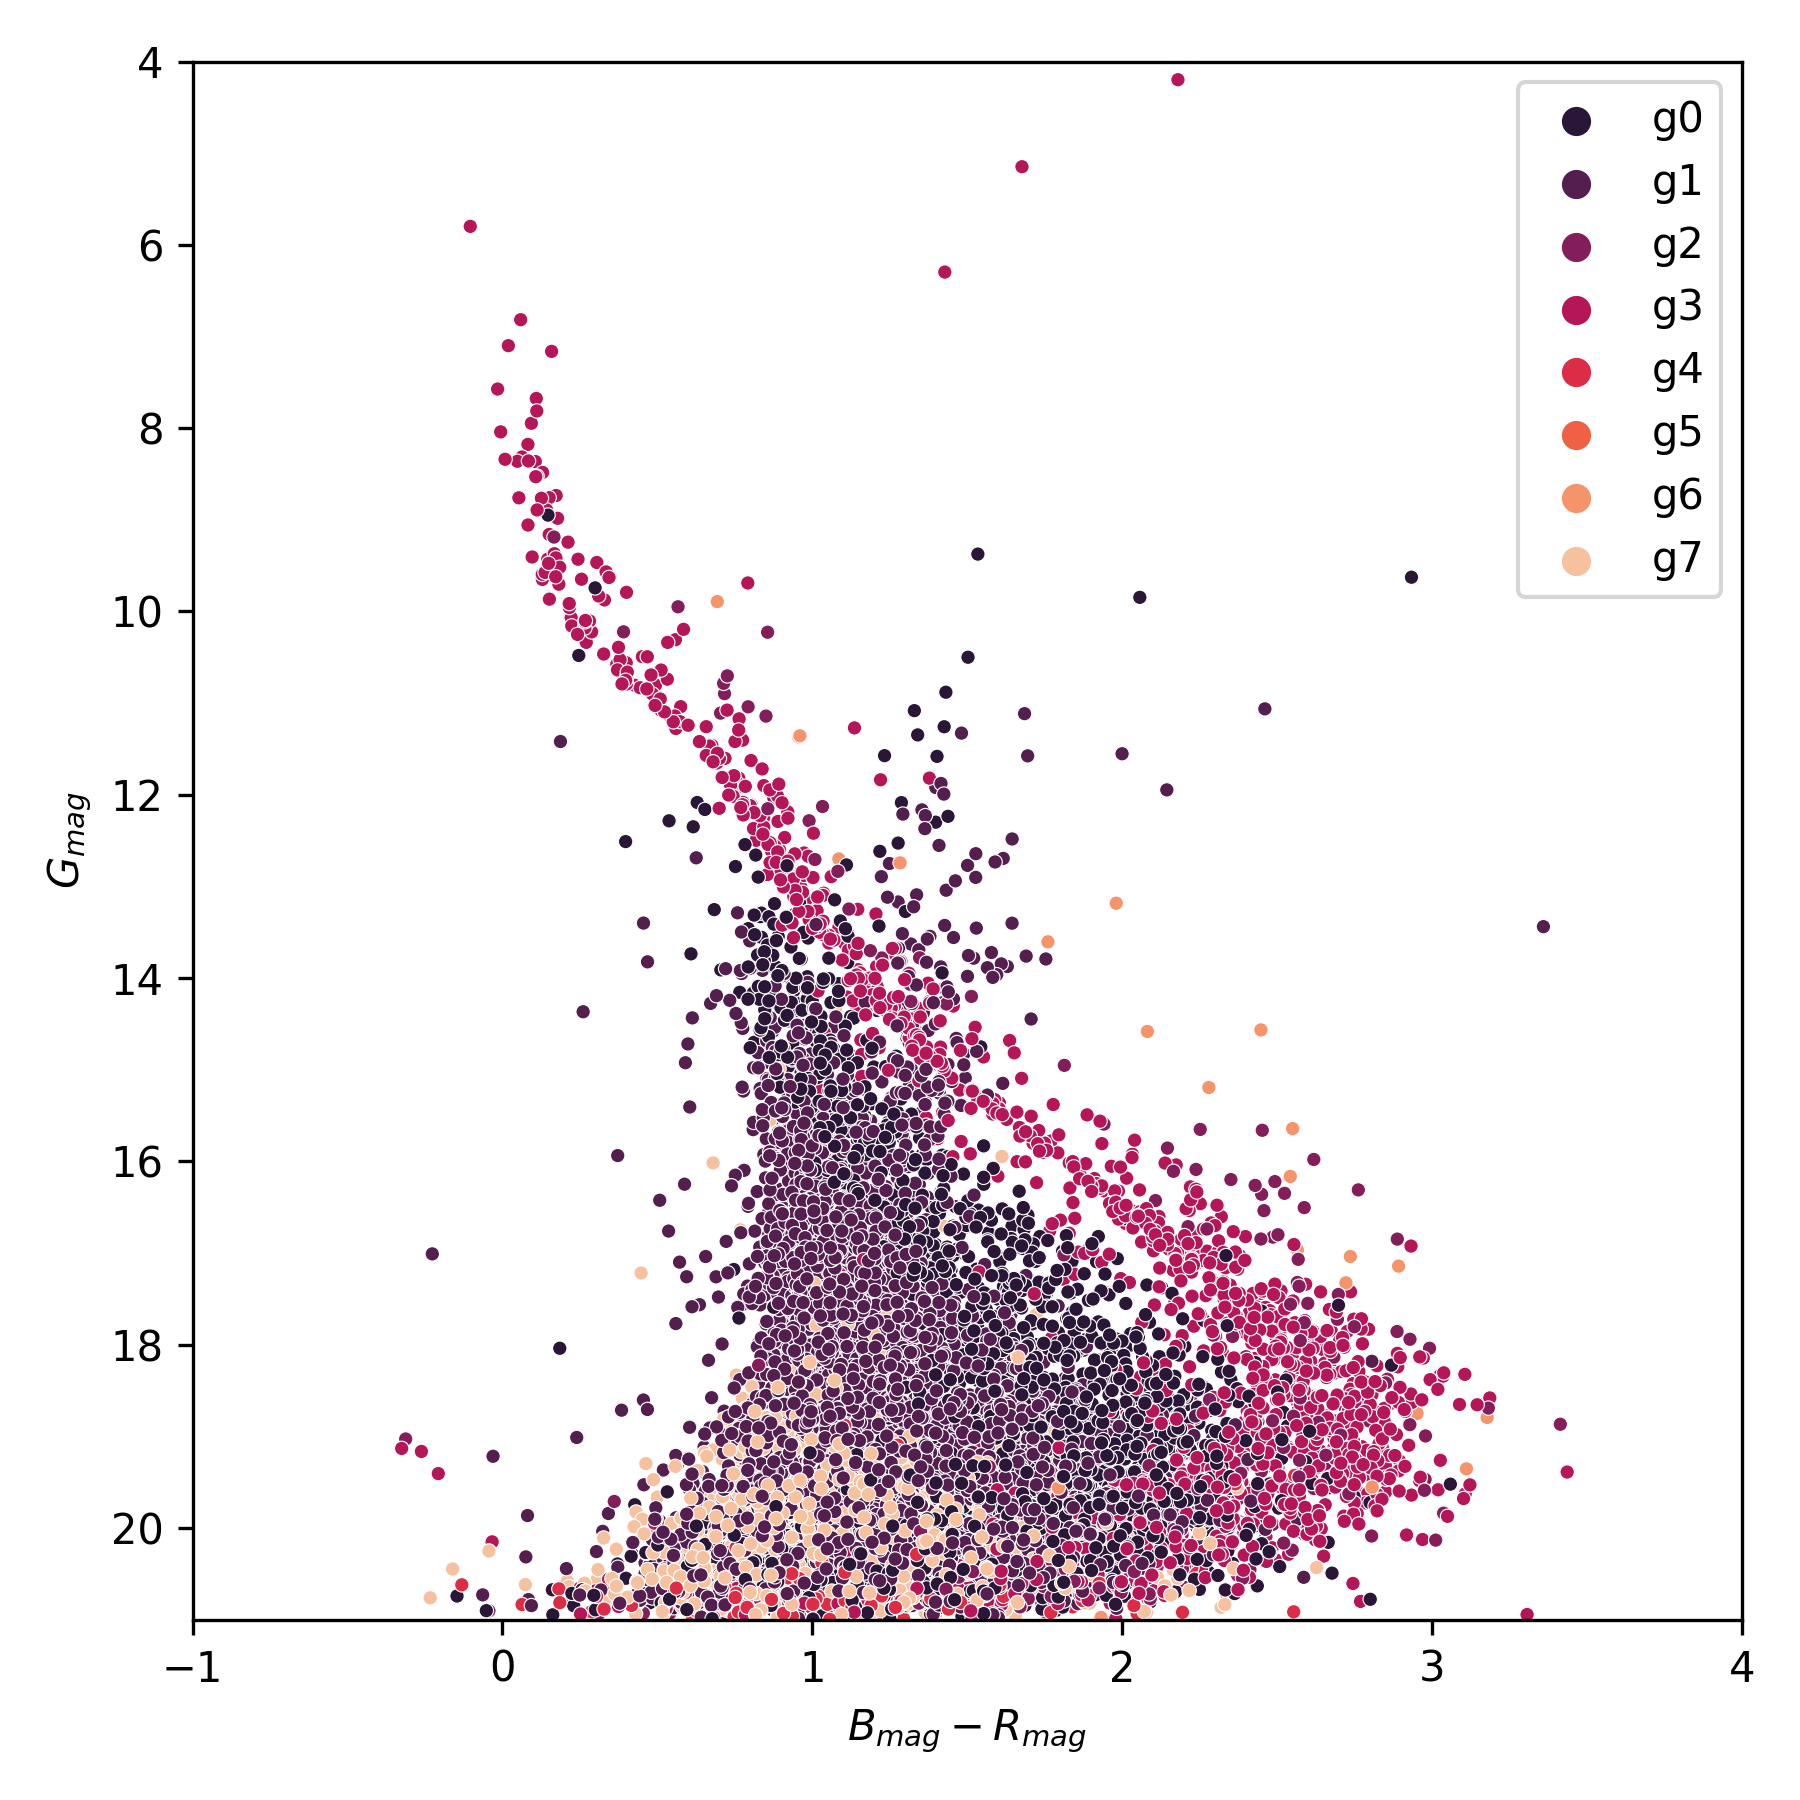
\includegraphics[width=\textwidth]{../figures/ngc_2516/kmeans_hr_diagram_ngc_2516.png}
    \end{subfigure}
  \end{subfigure}
  \caption{NGC 2516 characterization.
           Top: Clusterix+TOPCAT. Bottom: K-Means (\emph{g3}).}
  \label{fig:app_result_ngc_2516_clusterix_kmeans}
\end{figure}

Figure~\ref{fig:app_result_ngc_2516_dec} shows the groups found using the
DEC model (top row) and the DEC model filtered (bottom row).
K-Means and DEC have labeled NGC 2516 as \emph{g3}. Although in general,
groups between K-Means and DEC models may not match.
Hyperparameters used in this characterization are listed in
Table~\ref{tab:app_hyperparameters_ngc_2516}.

\begin{figure}[htbp]
  \centering
  \begin{subfigure}{\columnwidth}
    \centering
    \begin{subfigure}[t]{0.30\textwidth}
      \centering
      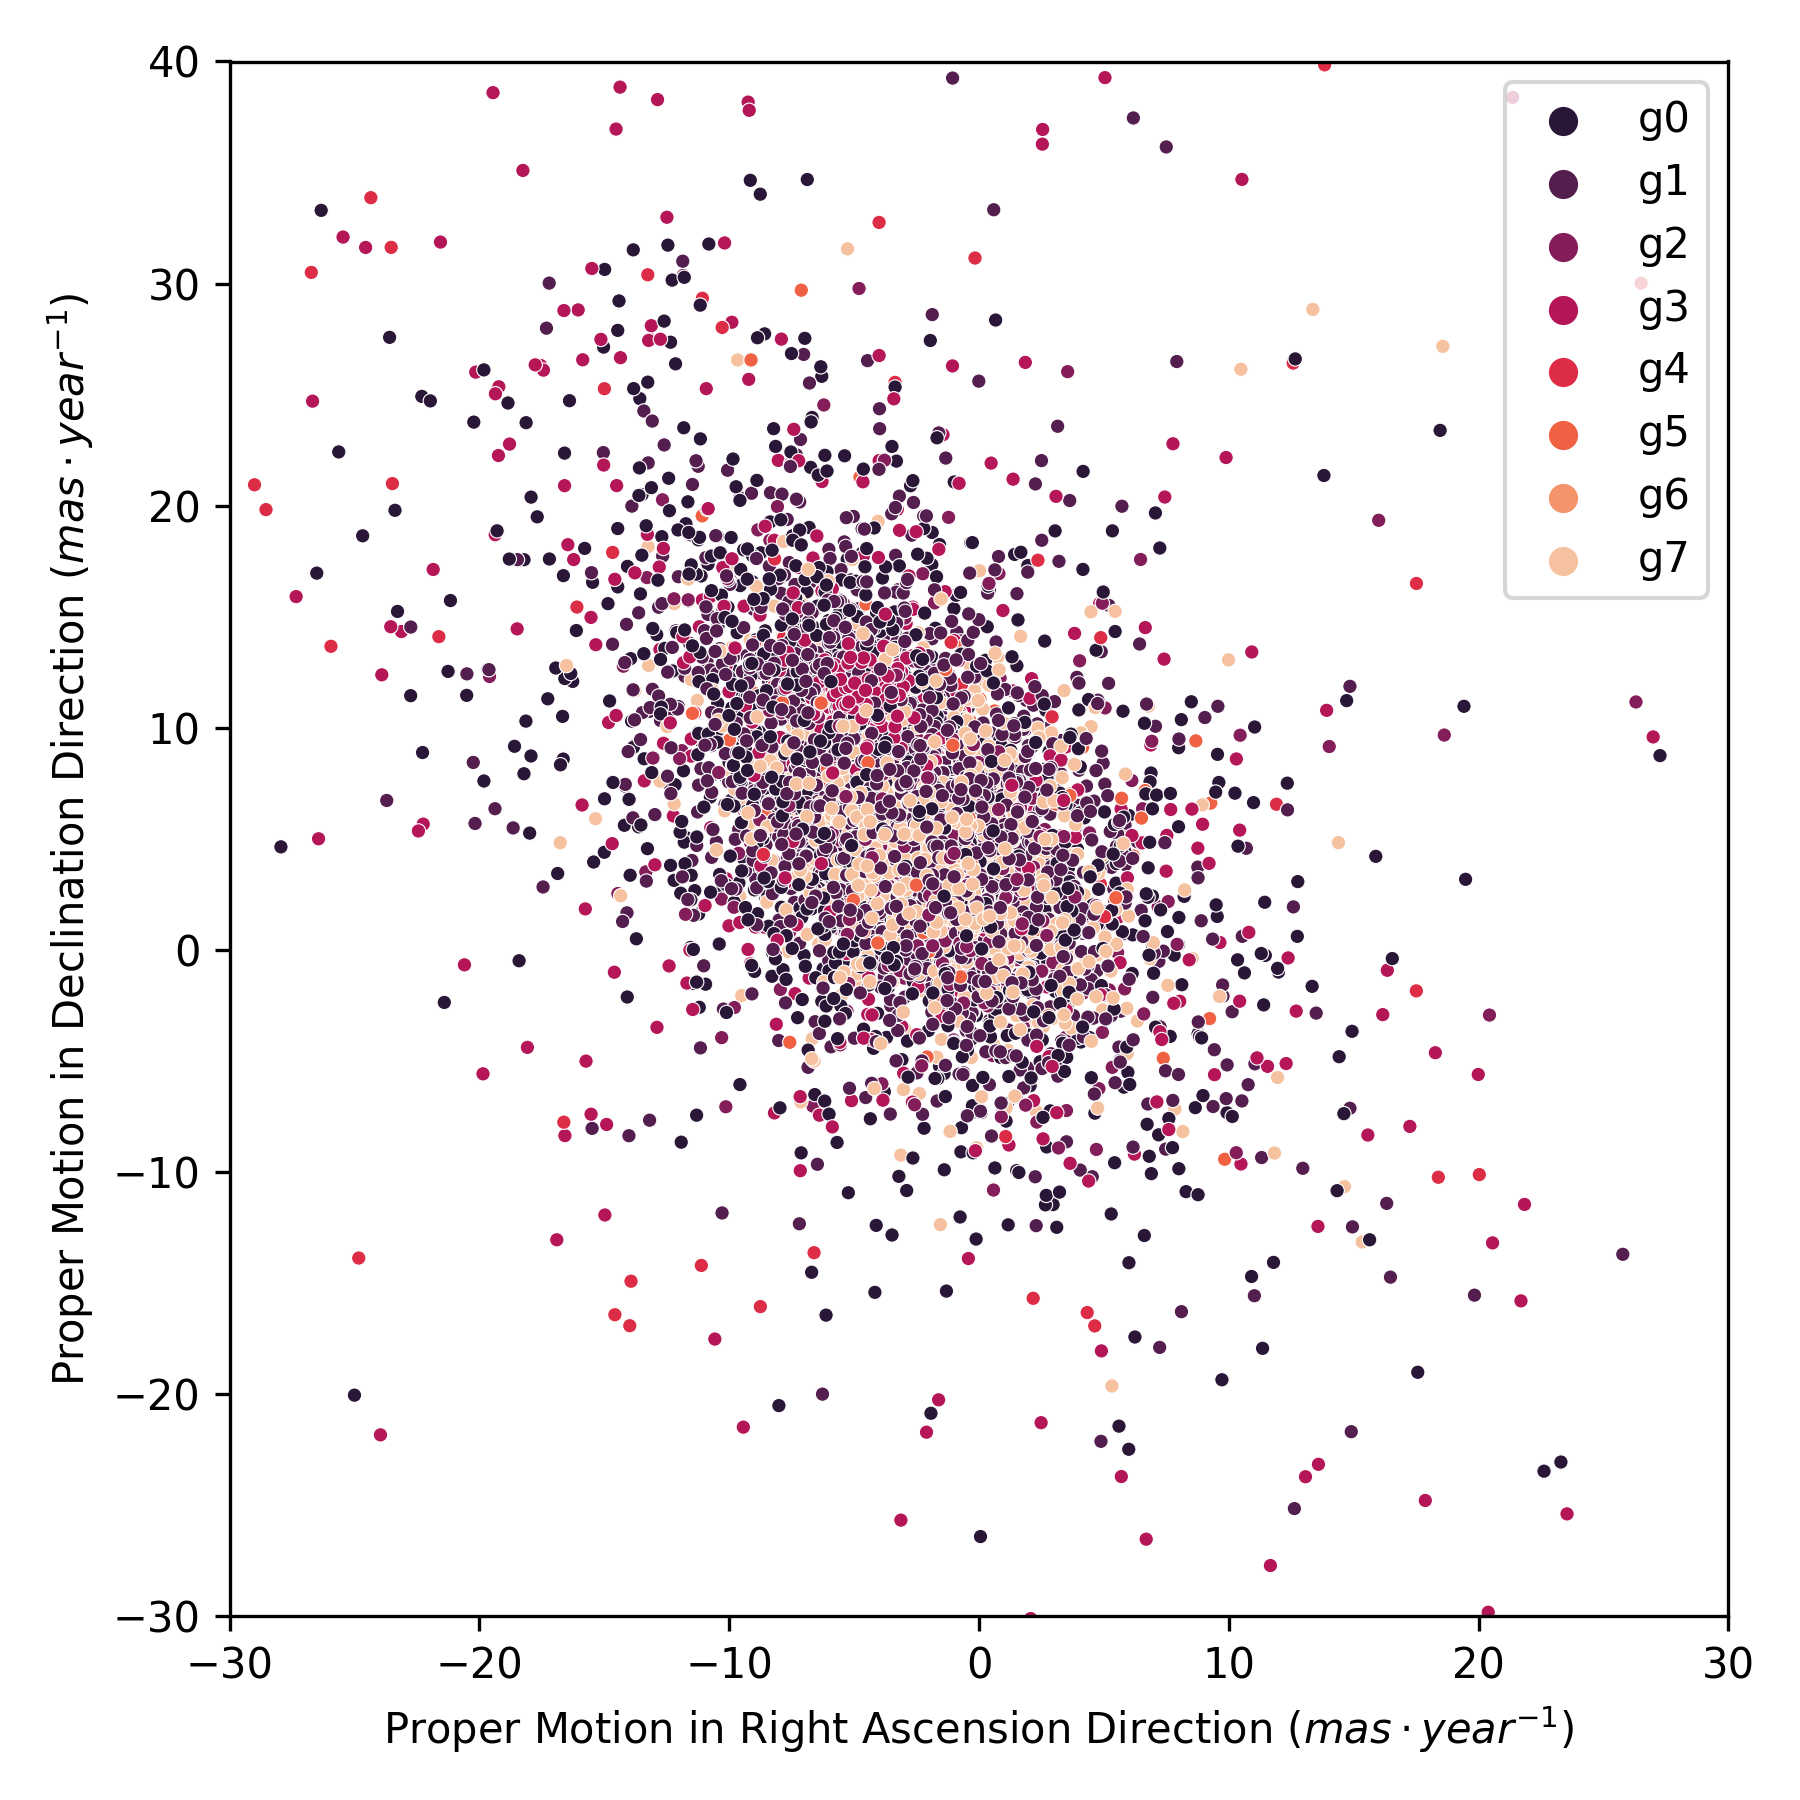
\includegraphics[width=\textwidth]{../figures/ngc_2516/dec_pm_ngc_2516.png}
    \end{subfigure}
    \hfill
    \begin{subfigure}[t]{0.30\textwidth}
      \centering
      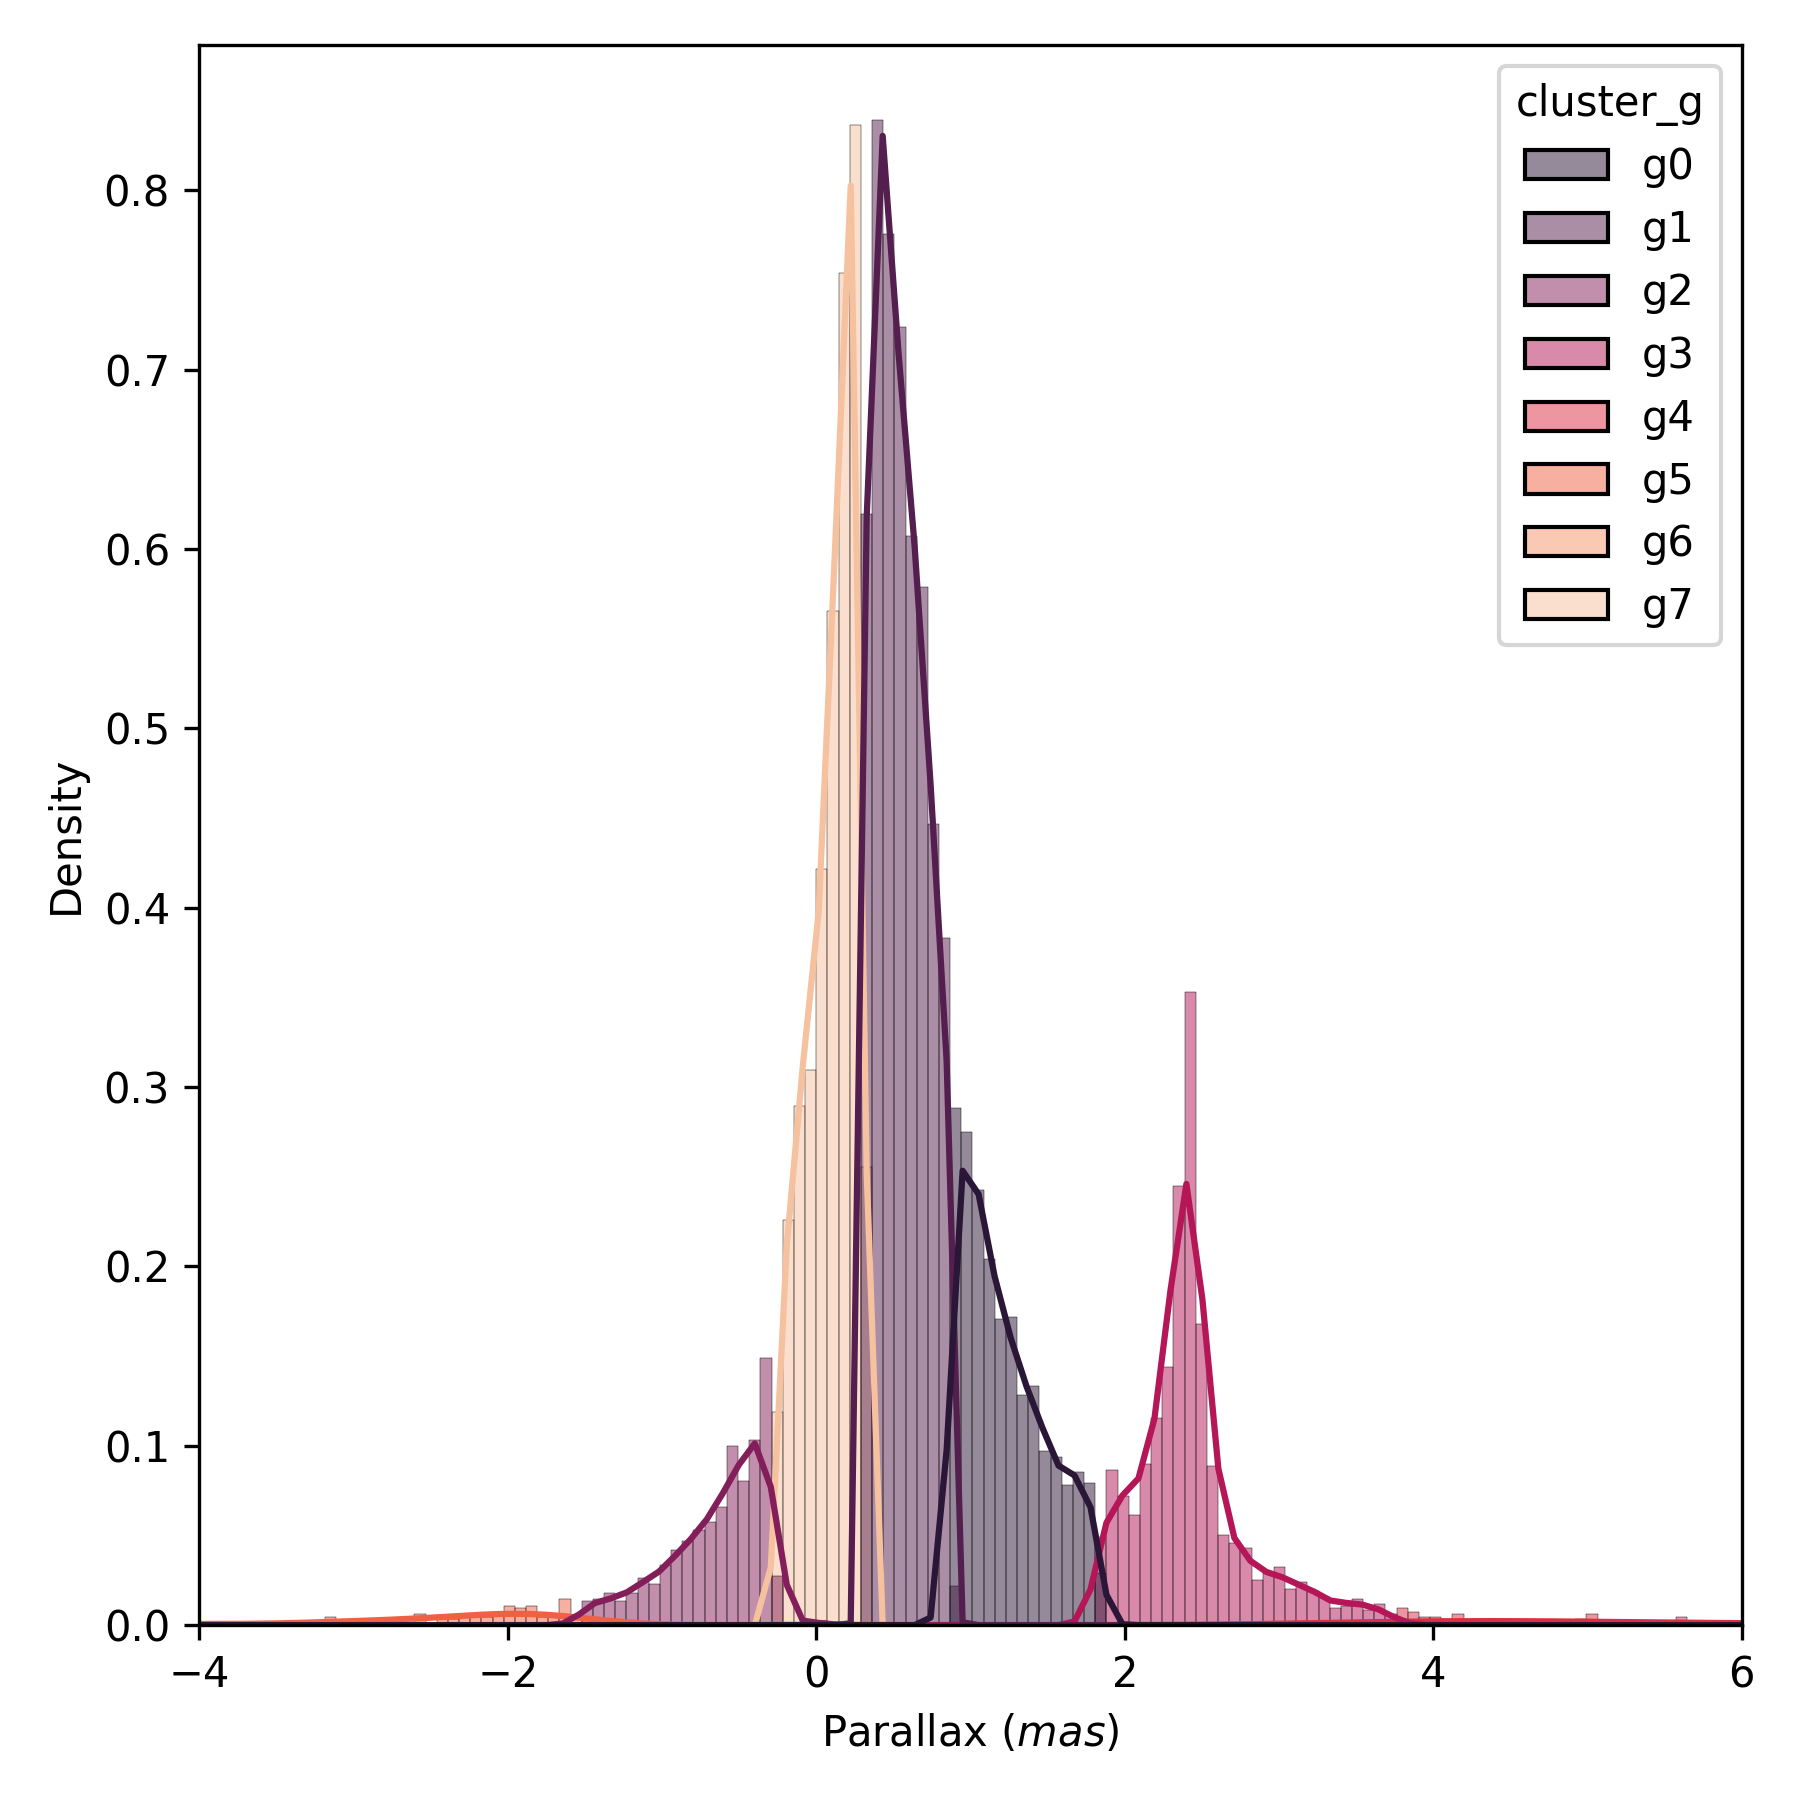
\includegraphics[width=\textwidth]{../figures/ngc_2516/dec_parallax_ngc_2516.png}
    \end{subfigure}
    \hfill
    \begin{subfigure}[t]{0.30\textwidth}
      \centering
      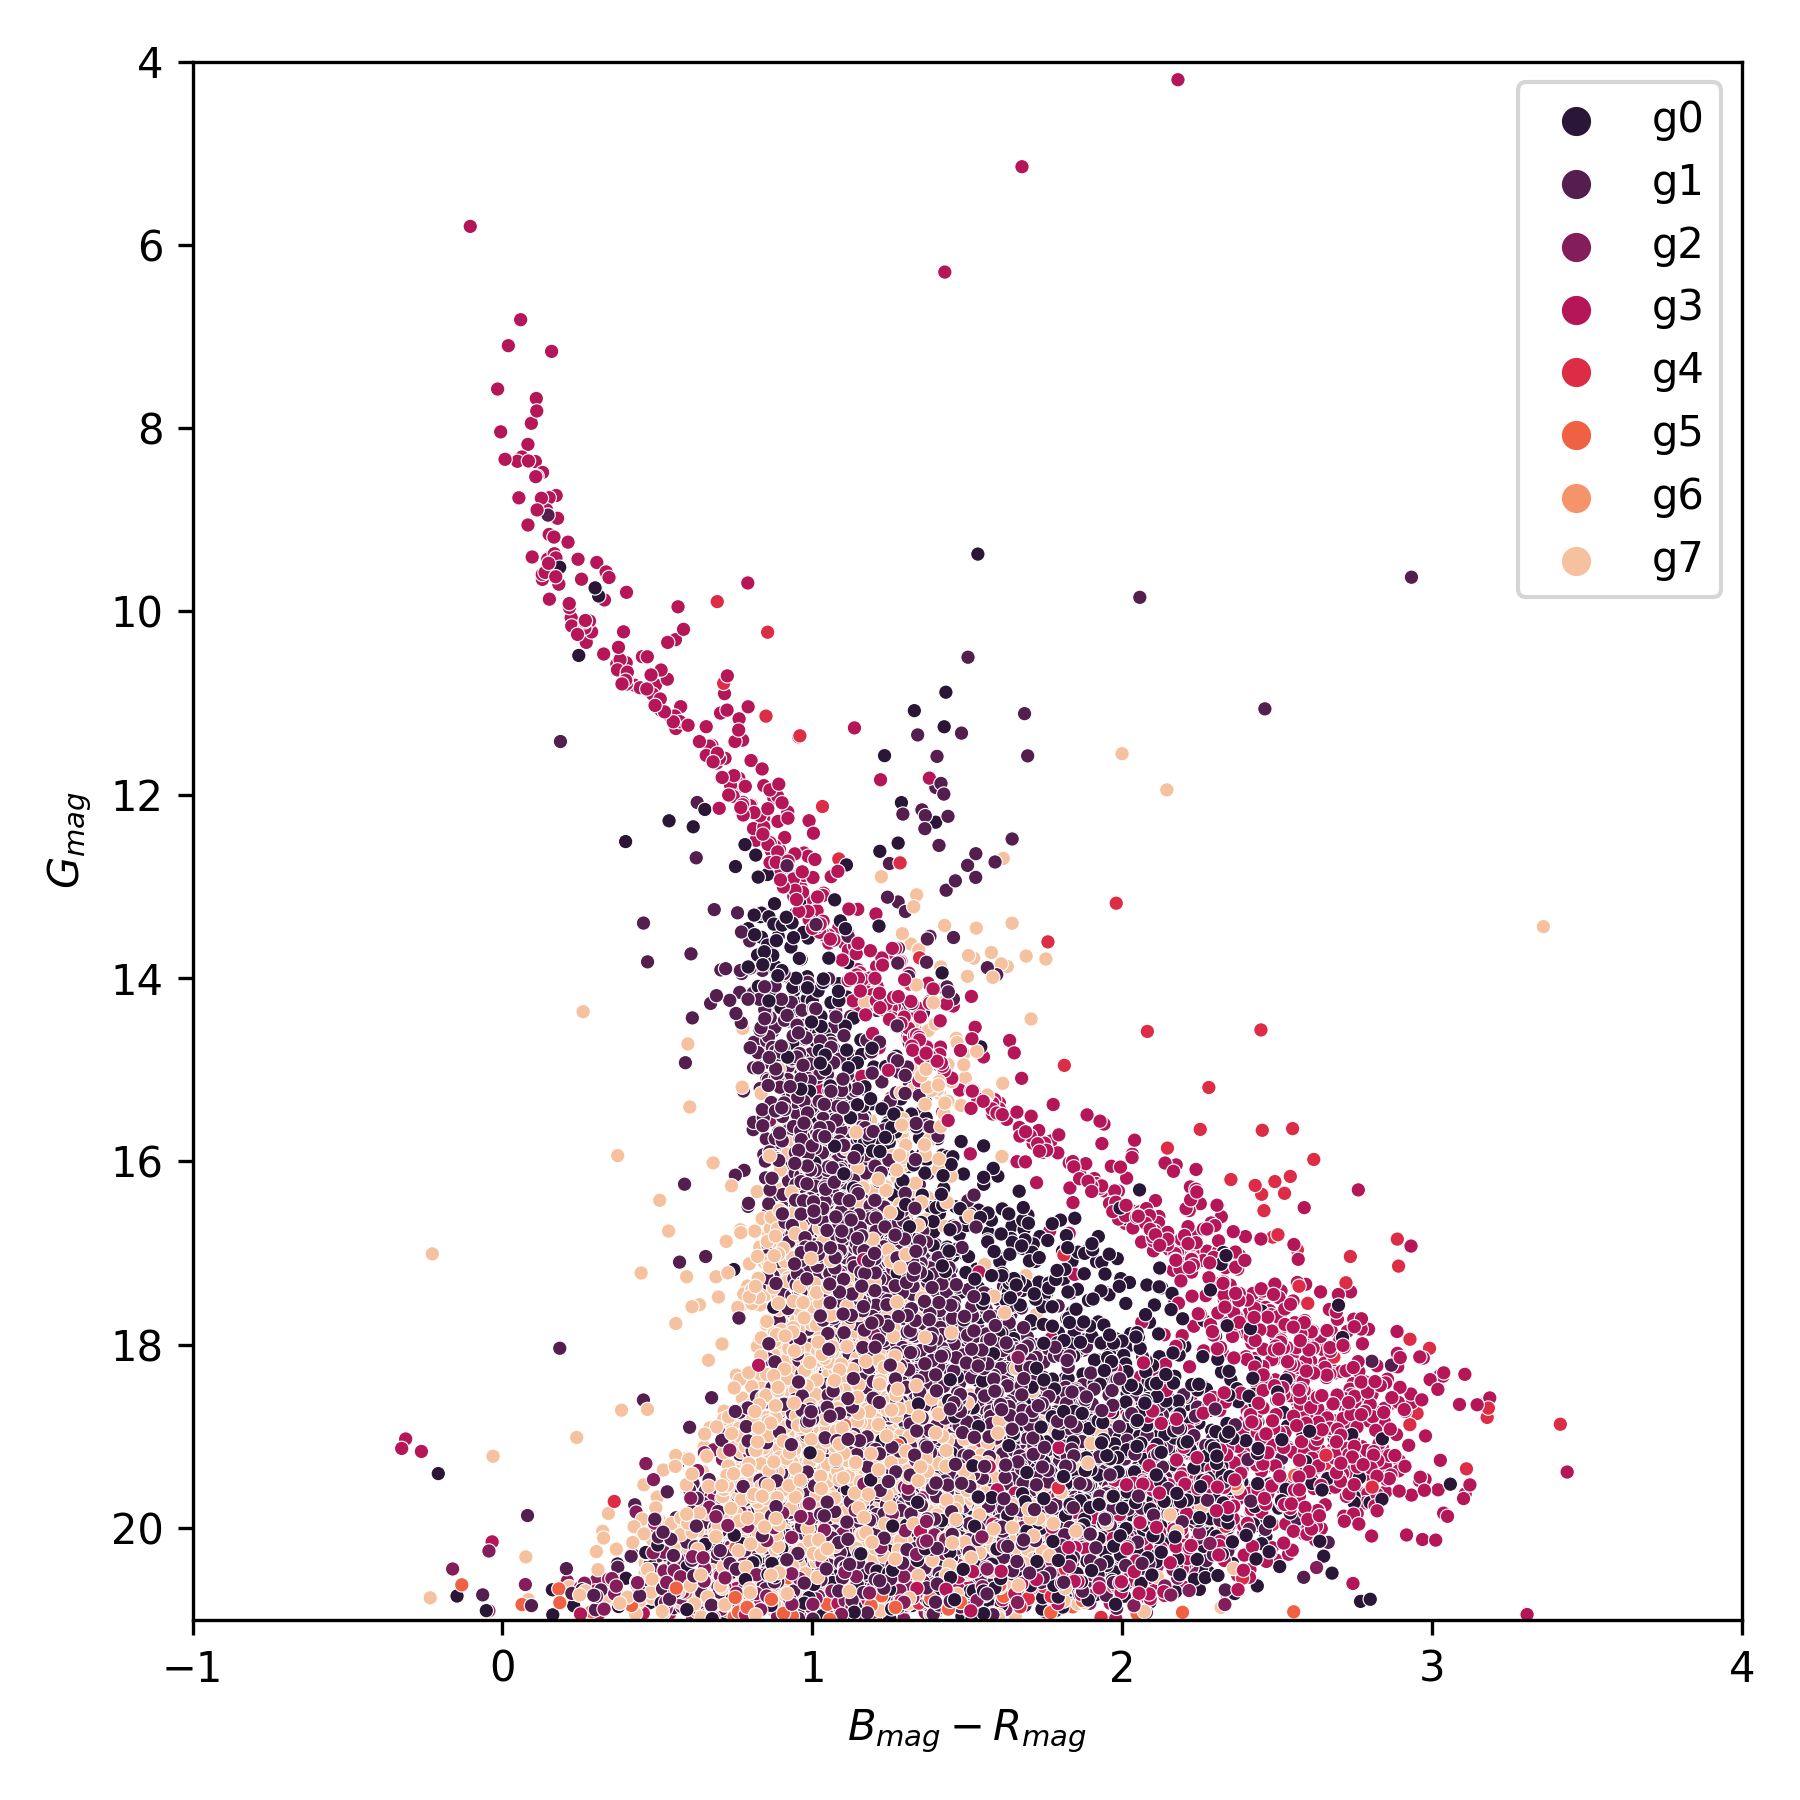
\includegraphics[width=\textwidth]{../figures/ngc_2516/dec_hr_diagram_ngc_2516.png}
    \end{subfigure}
  \end{subfigure}
  \centering
  \begin{subfigure}{\columnwidth}
    \centering
    \begin{subfigure}[t]{0.30\textwidth}
      \centering
      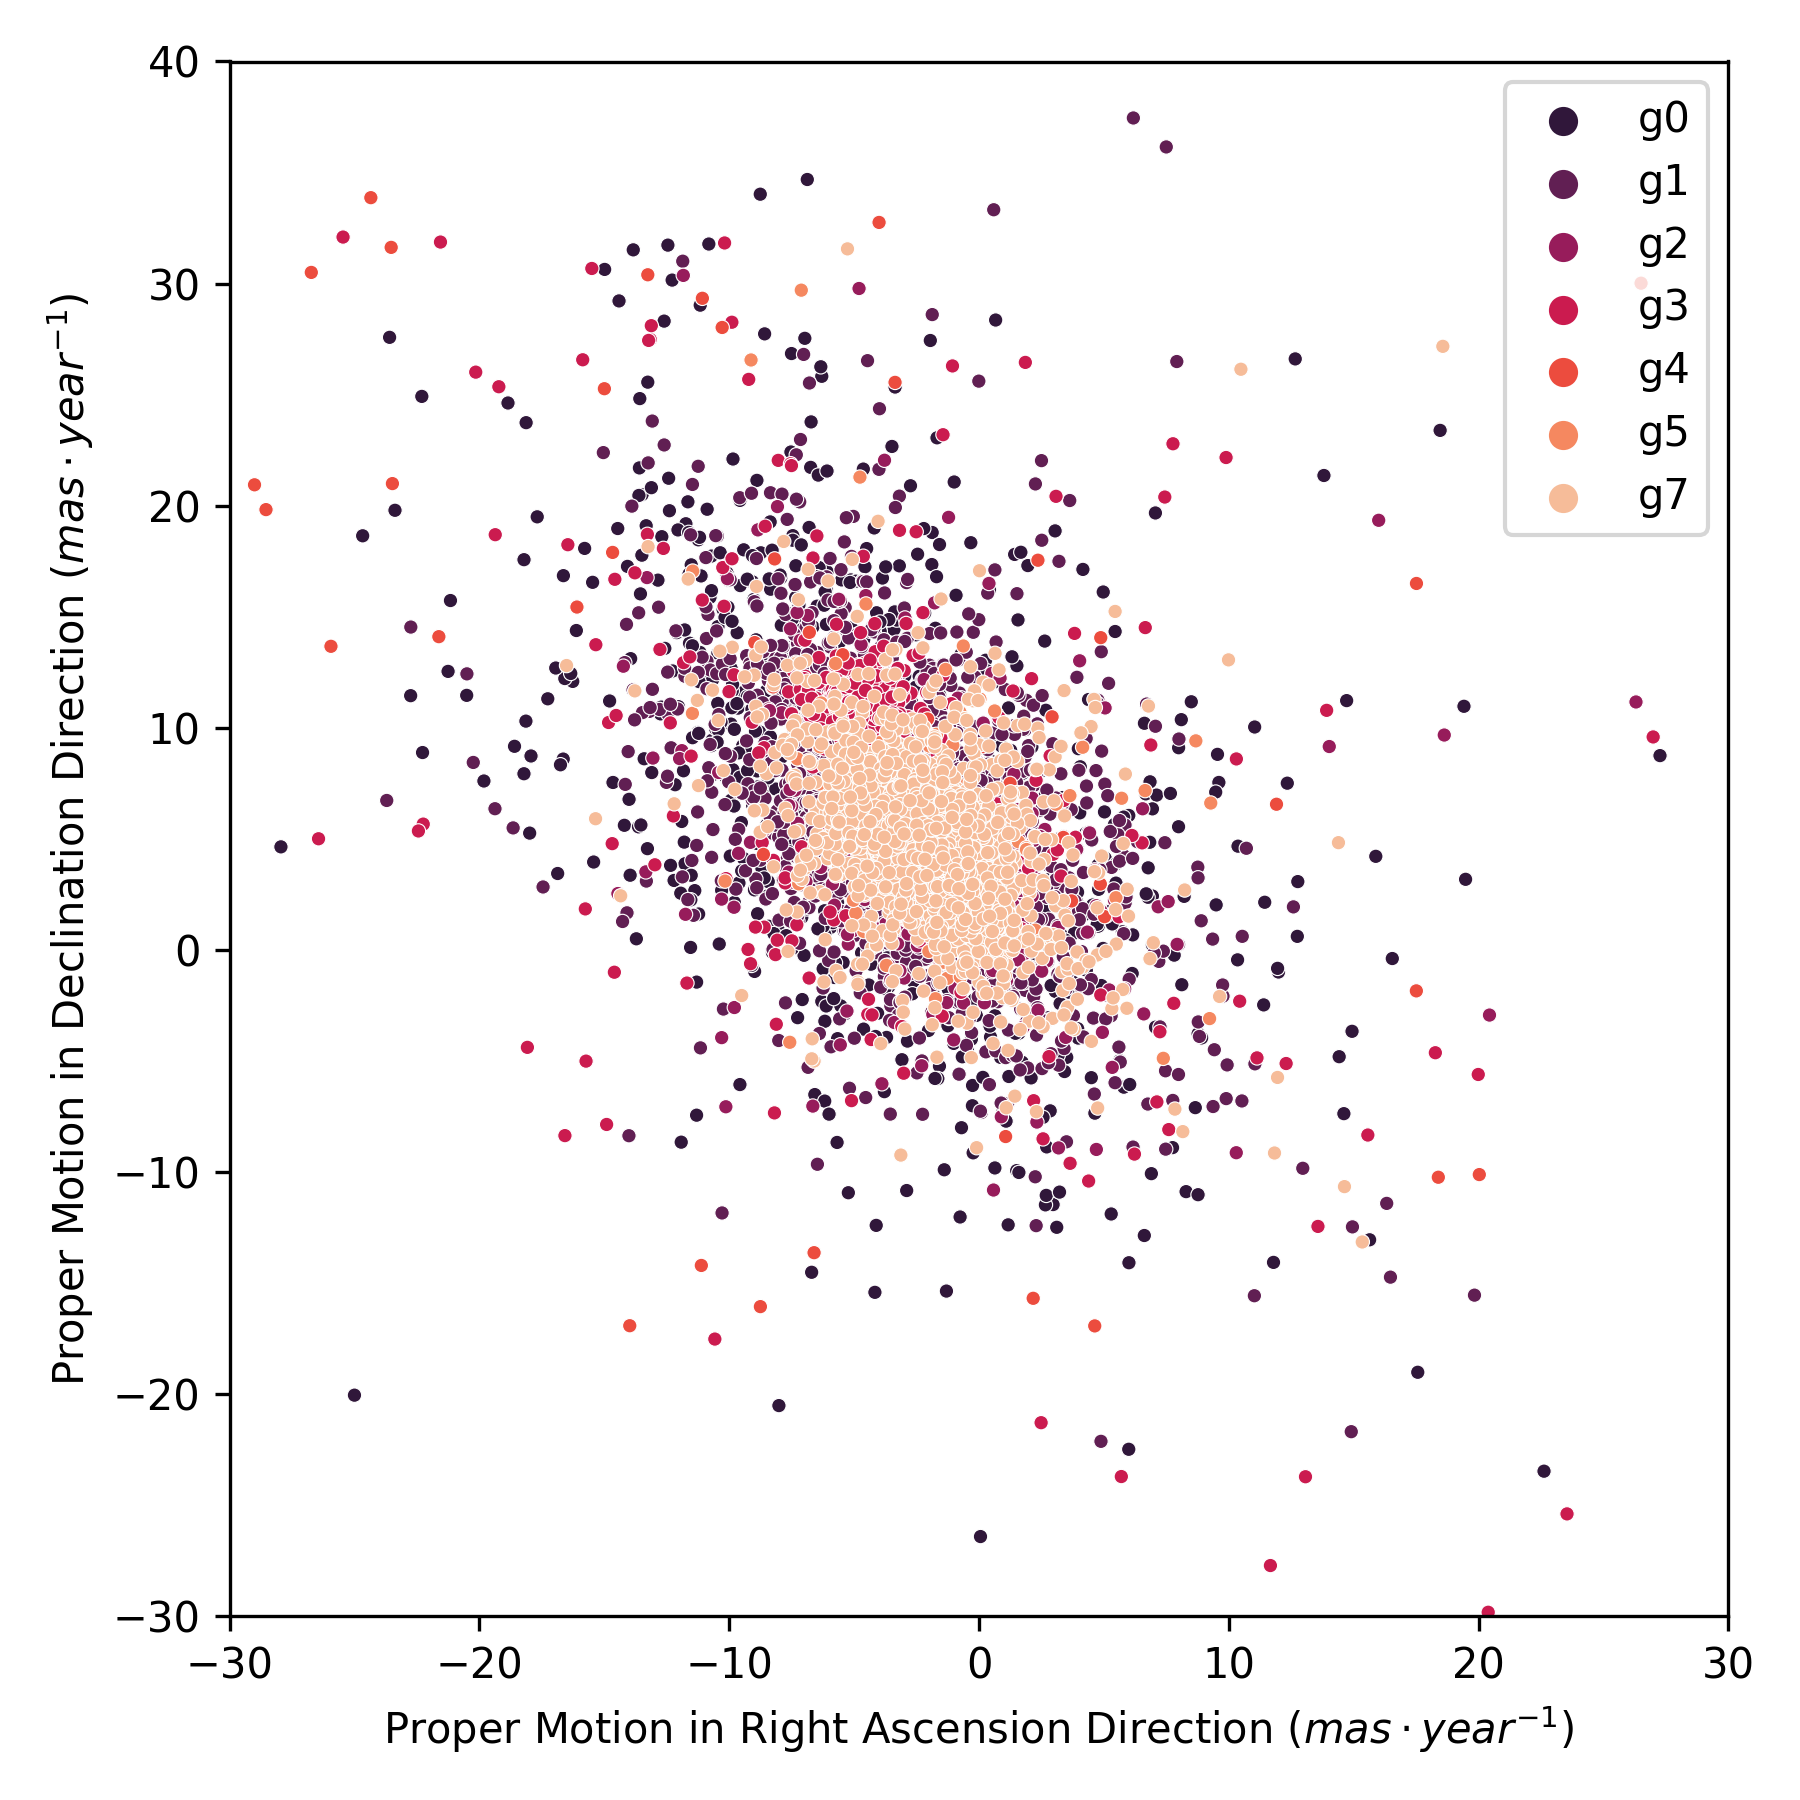
\includegraphics[width=\textwidth]{../figures/ngc_2516/dec_pm_filtered_ngc_2516.png}
    \end{subfigure}
    \hfill
    \begin{subfigure}[t]{0.30\textwidth}
      \centering
      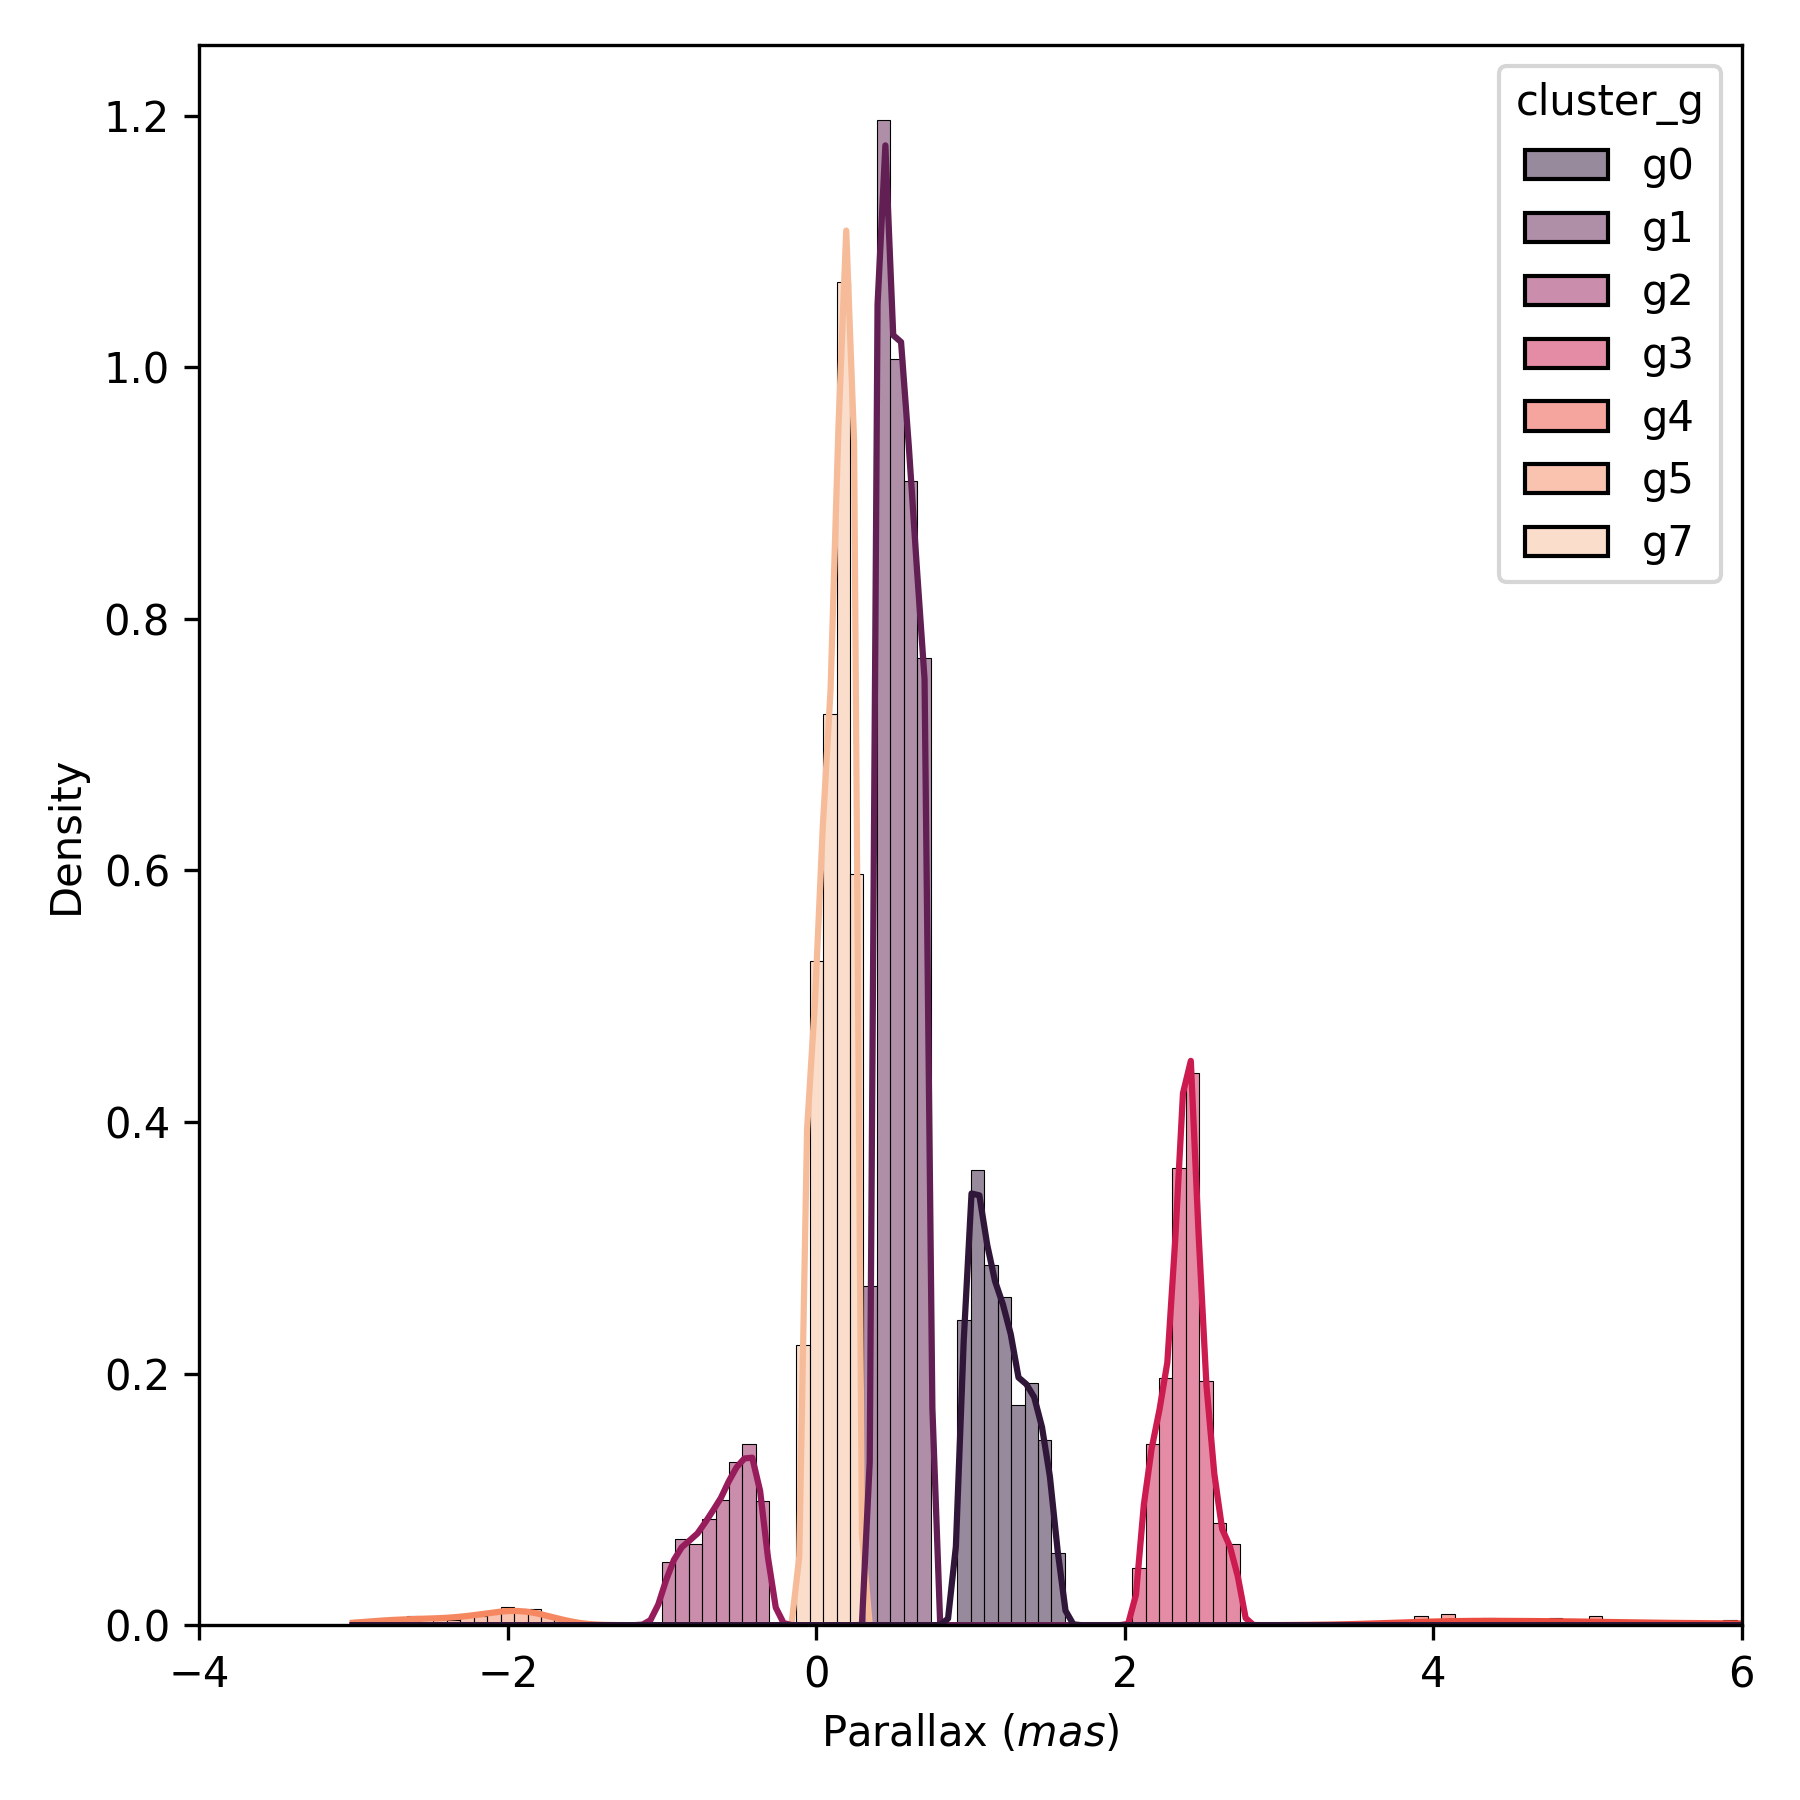
\includegraphics[width=\textwidth]{../figures/ngc_2516/dec_parallax_filtered_ngc_2516.png}
    \end{subfigure}
    \hfill
    \begin{subfigure}[t]{0.30\textwidth}
      \centering
      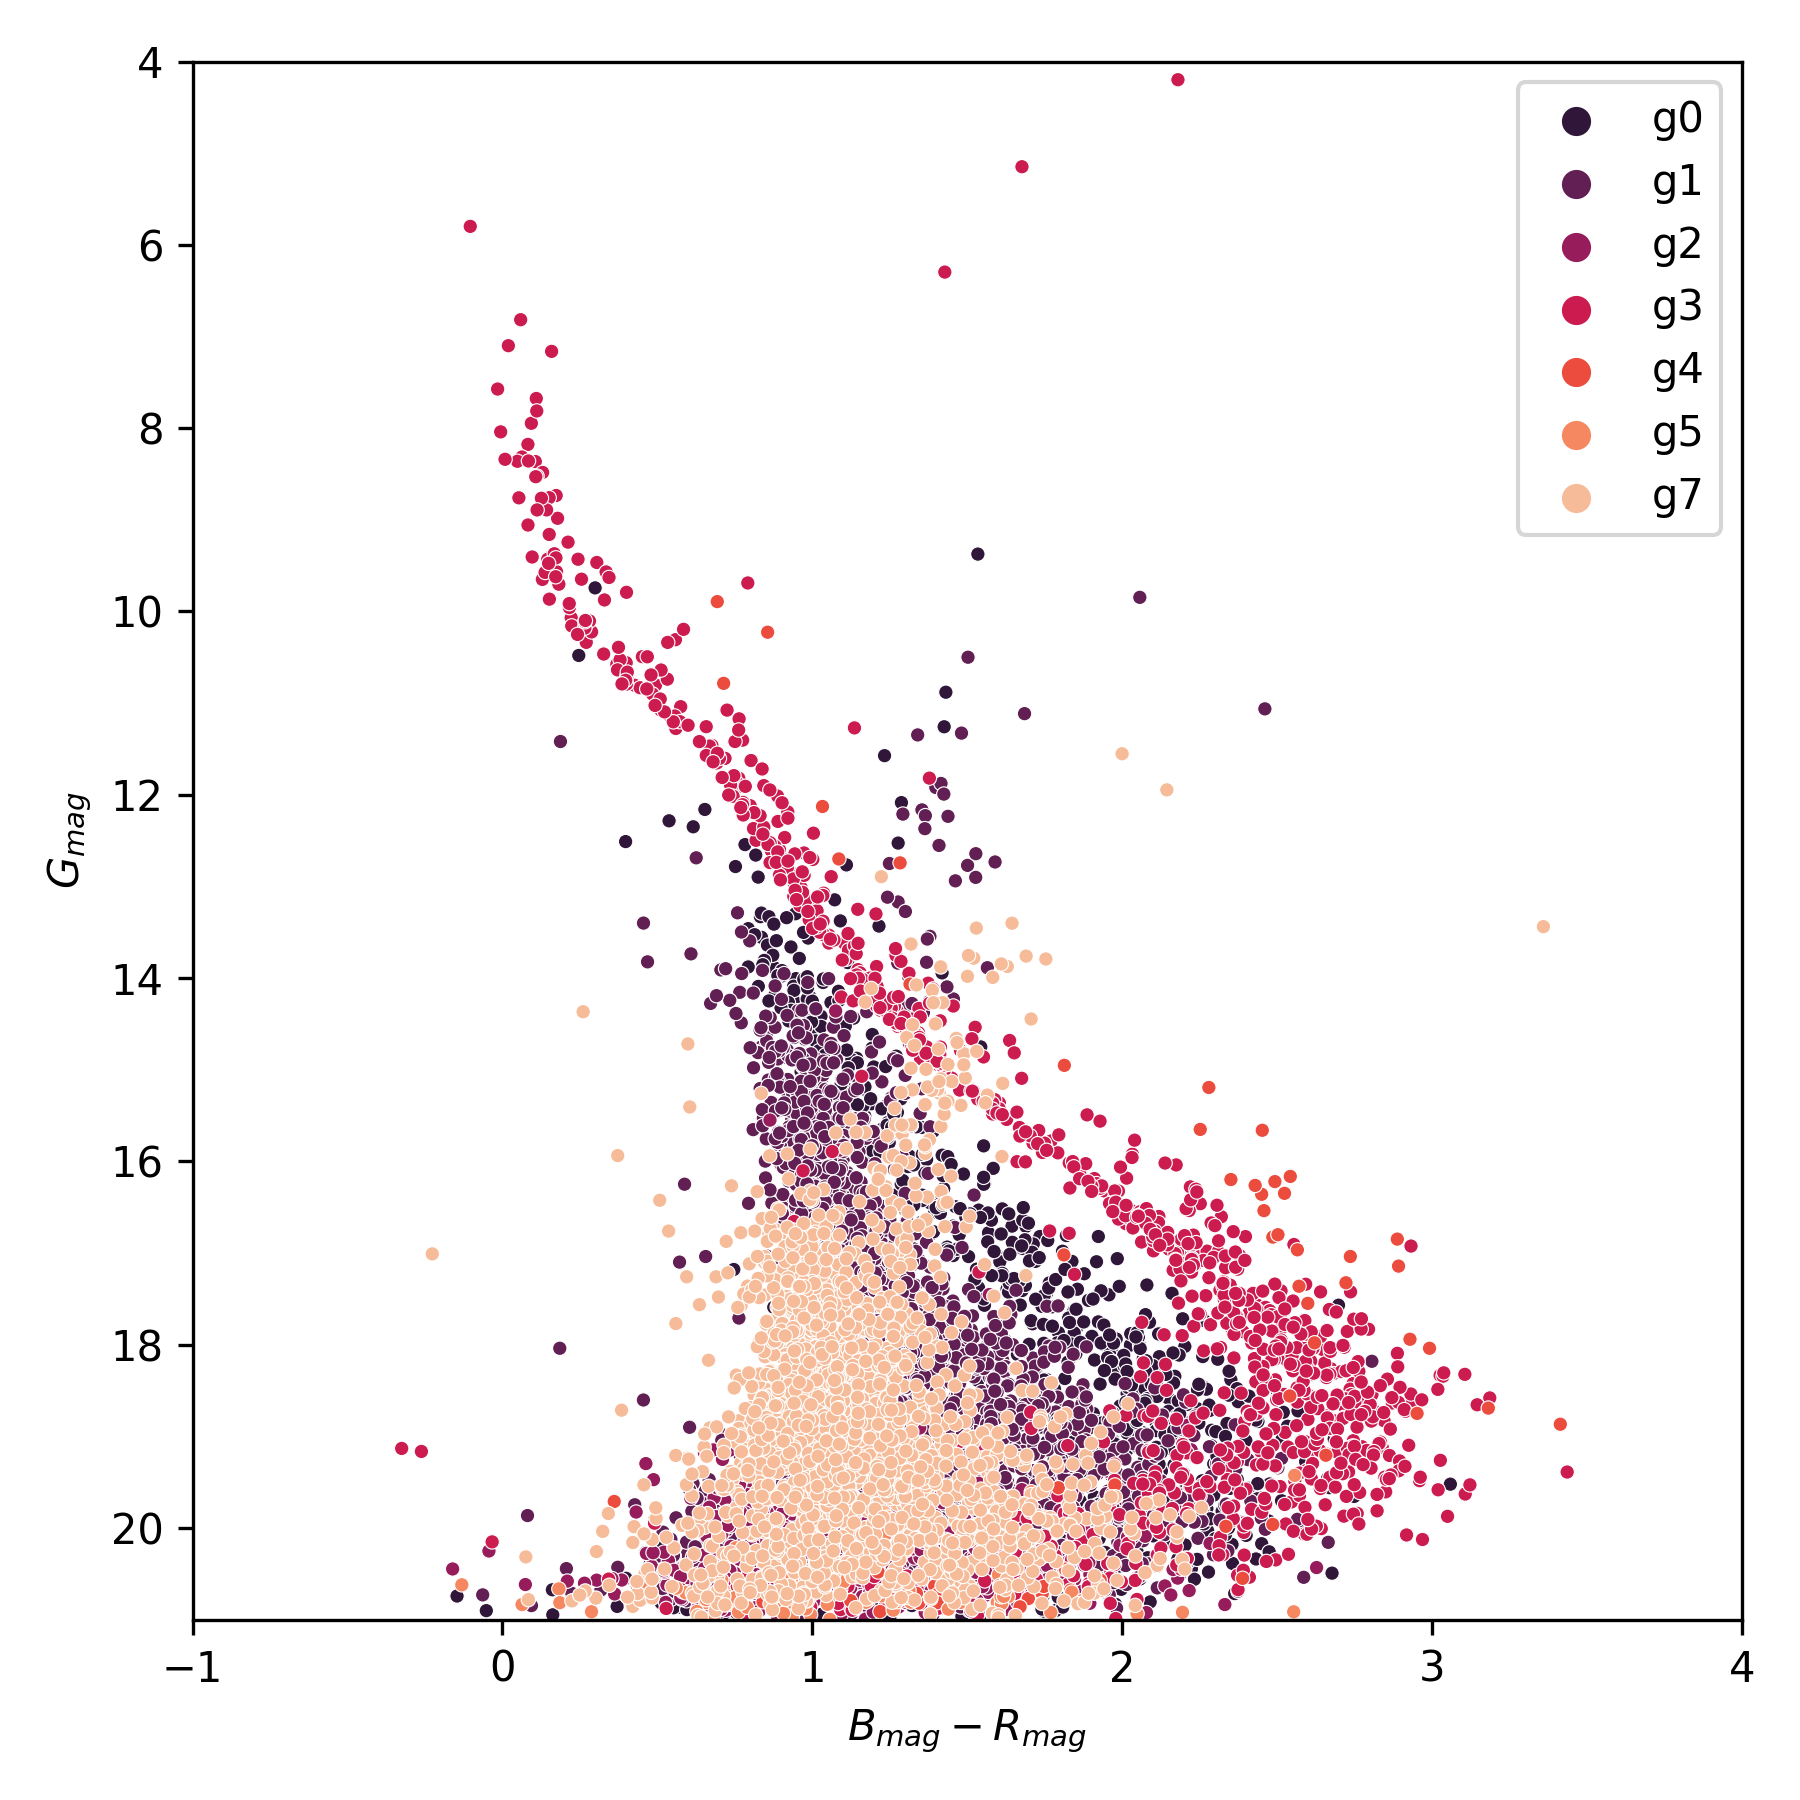
\includegraphics[width=\textwidth]{../figures/ngc_2516/dec_hr_diagram_filtered_ngc_2516.png}
    \end{subfigure}
  \end{subfigure}
  \caption{NGC 2516 characterization (labeled as \emph{g3}).
           DEC (top). DEC filtered (bottom).}
  \label{fig:app_result_ngc_2516_dec}
\end{figure}

\begin{table}[htbp]
  \begin{center}
    \begin{tabular}{l|c}
      \textbf{Hyperparameter} & \textbf{Value} \\
      \hline
      Number of Clusters & 8 \\
      Clustering Layer & \(\left[ 50, 50, 60 \right]\) \\
      Kernel Initializer Seed & 2 \\
      Quantil Threshold & 0.15 \\
    \end{tabular}
    \caption{NGC 2516 DEC hyperparameters.}
    \label{tab:app_hyperparameters_ngc_2516}
  \end{center}
\end{table}

\subsection{NGC 2632}
\label{sec:ngc2632}

Figure~\ref{fig:app_result_ngc_2632_clusterix_kmeans} shows NGC 2632 characterized
by the validation method (first row) and the characterization made by K-Means
showing ten clusters (second row). K-Means labels NGC 2632 as \emph{g1}.

\begin{figure}[htbp]
  \centering
  \begin{subfigure}{\columnwidth}
    \centering
    \begin{subfigure}[t]{0.30\textwidth}
      \centering
      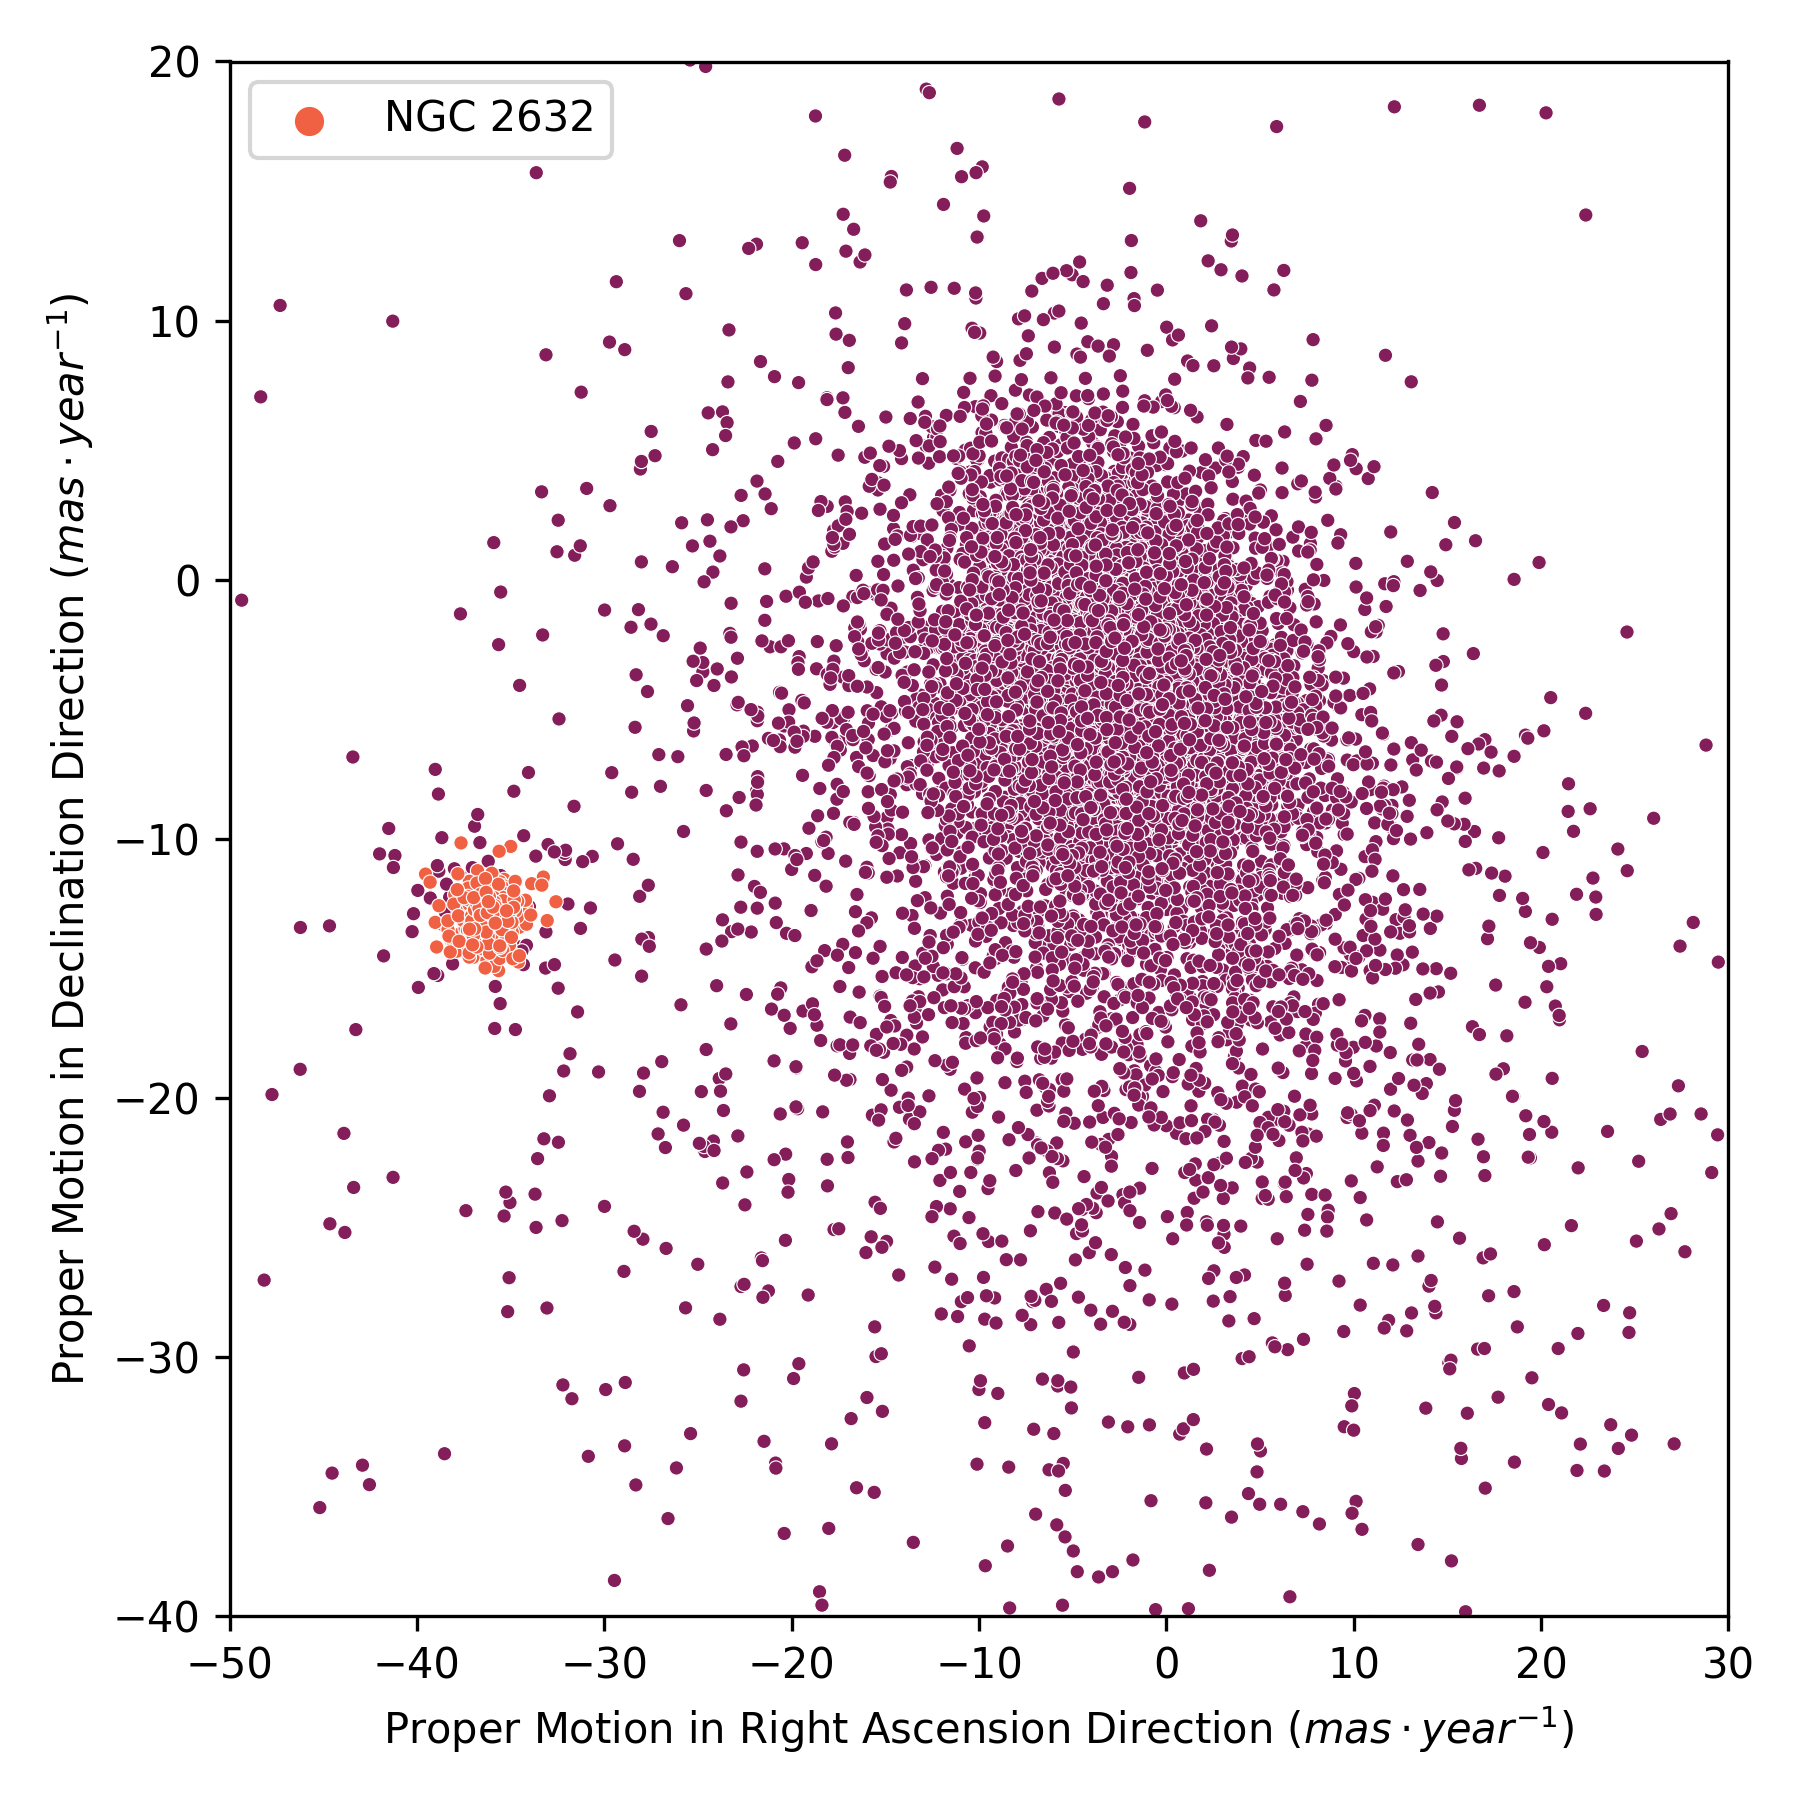
\includegraphics[width=\textwidth]{../figures/ngc_2632/pm_ngc_2632.png}
    \end{subfigure}
    \hfill
    \begin{subfigure}[t]{0.30\textwidth}
      \centering
      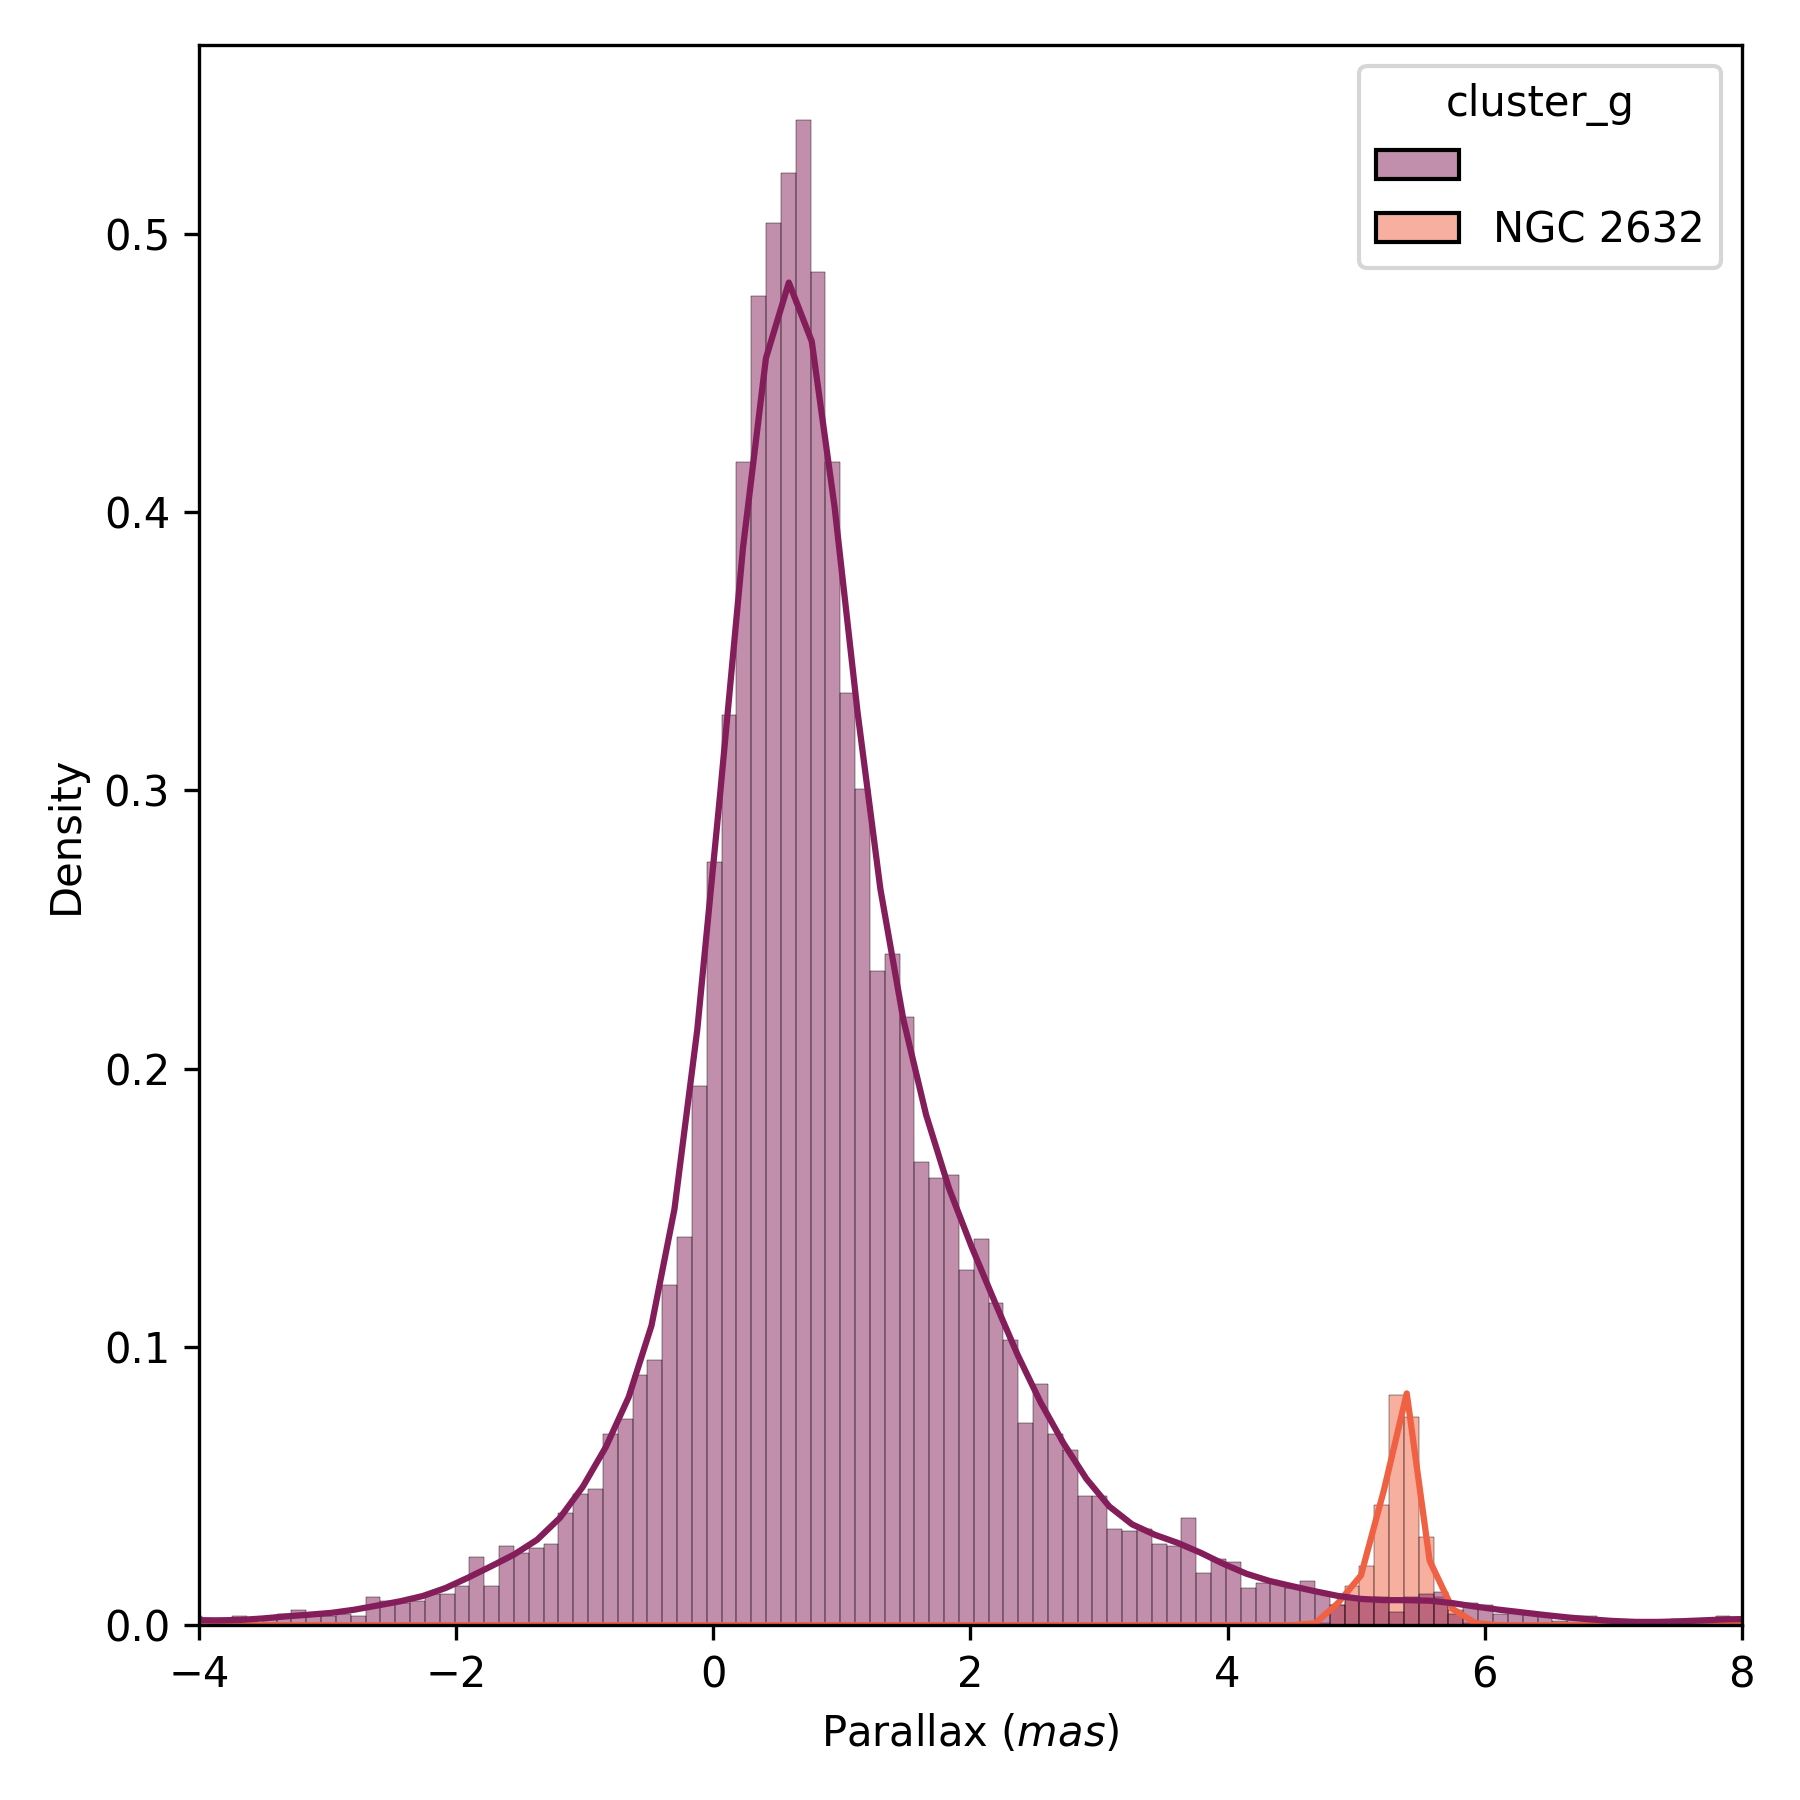
\includegraphics[width=\textwidth]{../figures/ngc_2632/parallax_ngc_2632.png}
    \end{subfigure}
    \hfill
    \begin{subfigure}[t]{0.30\textwidth}
      \centering
      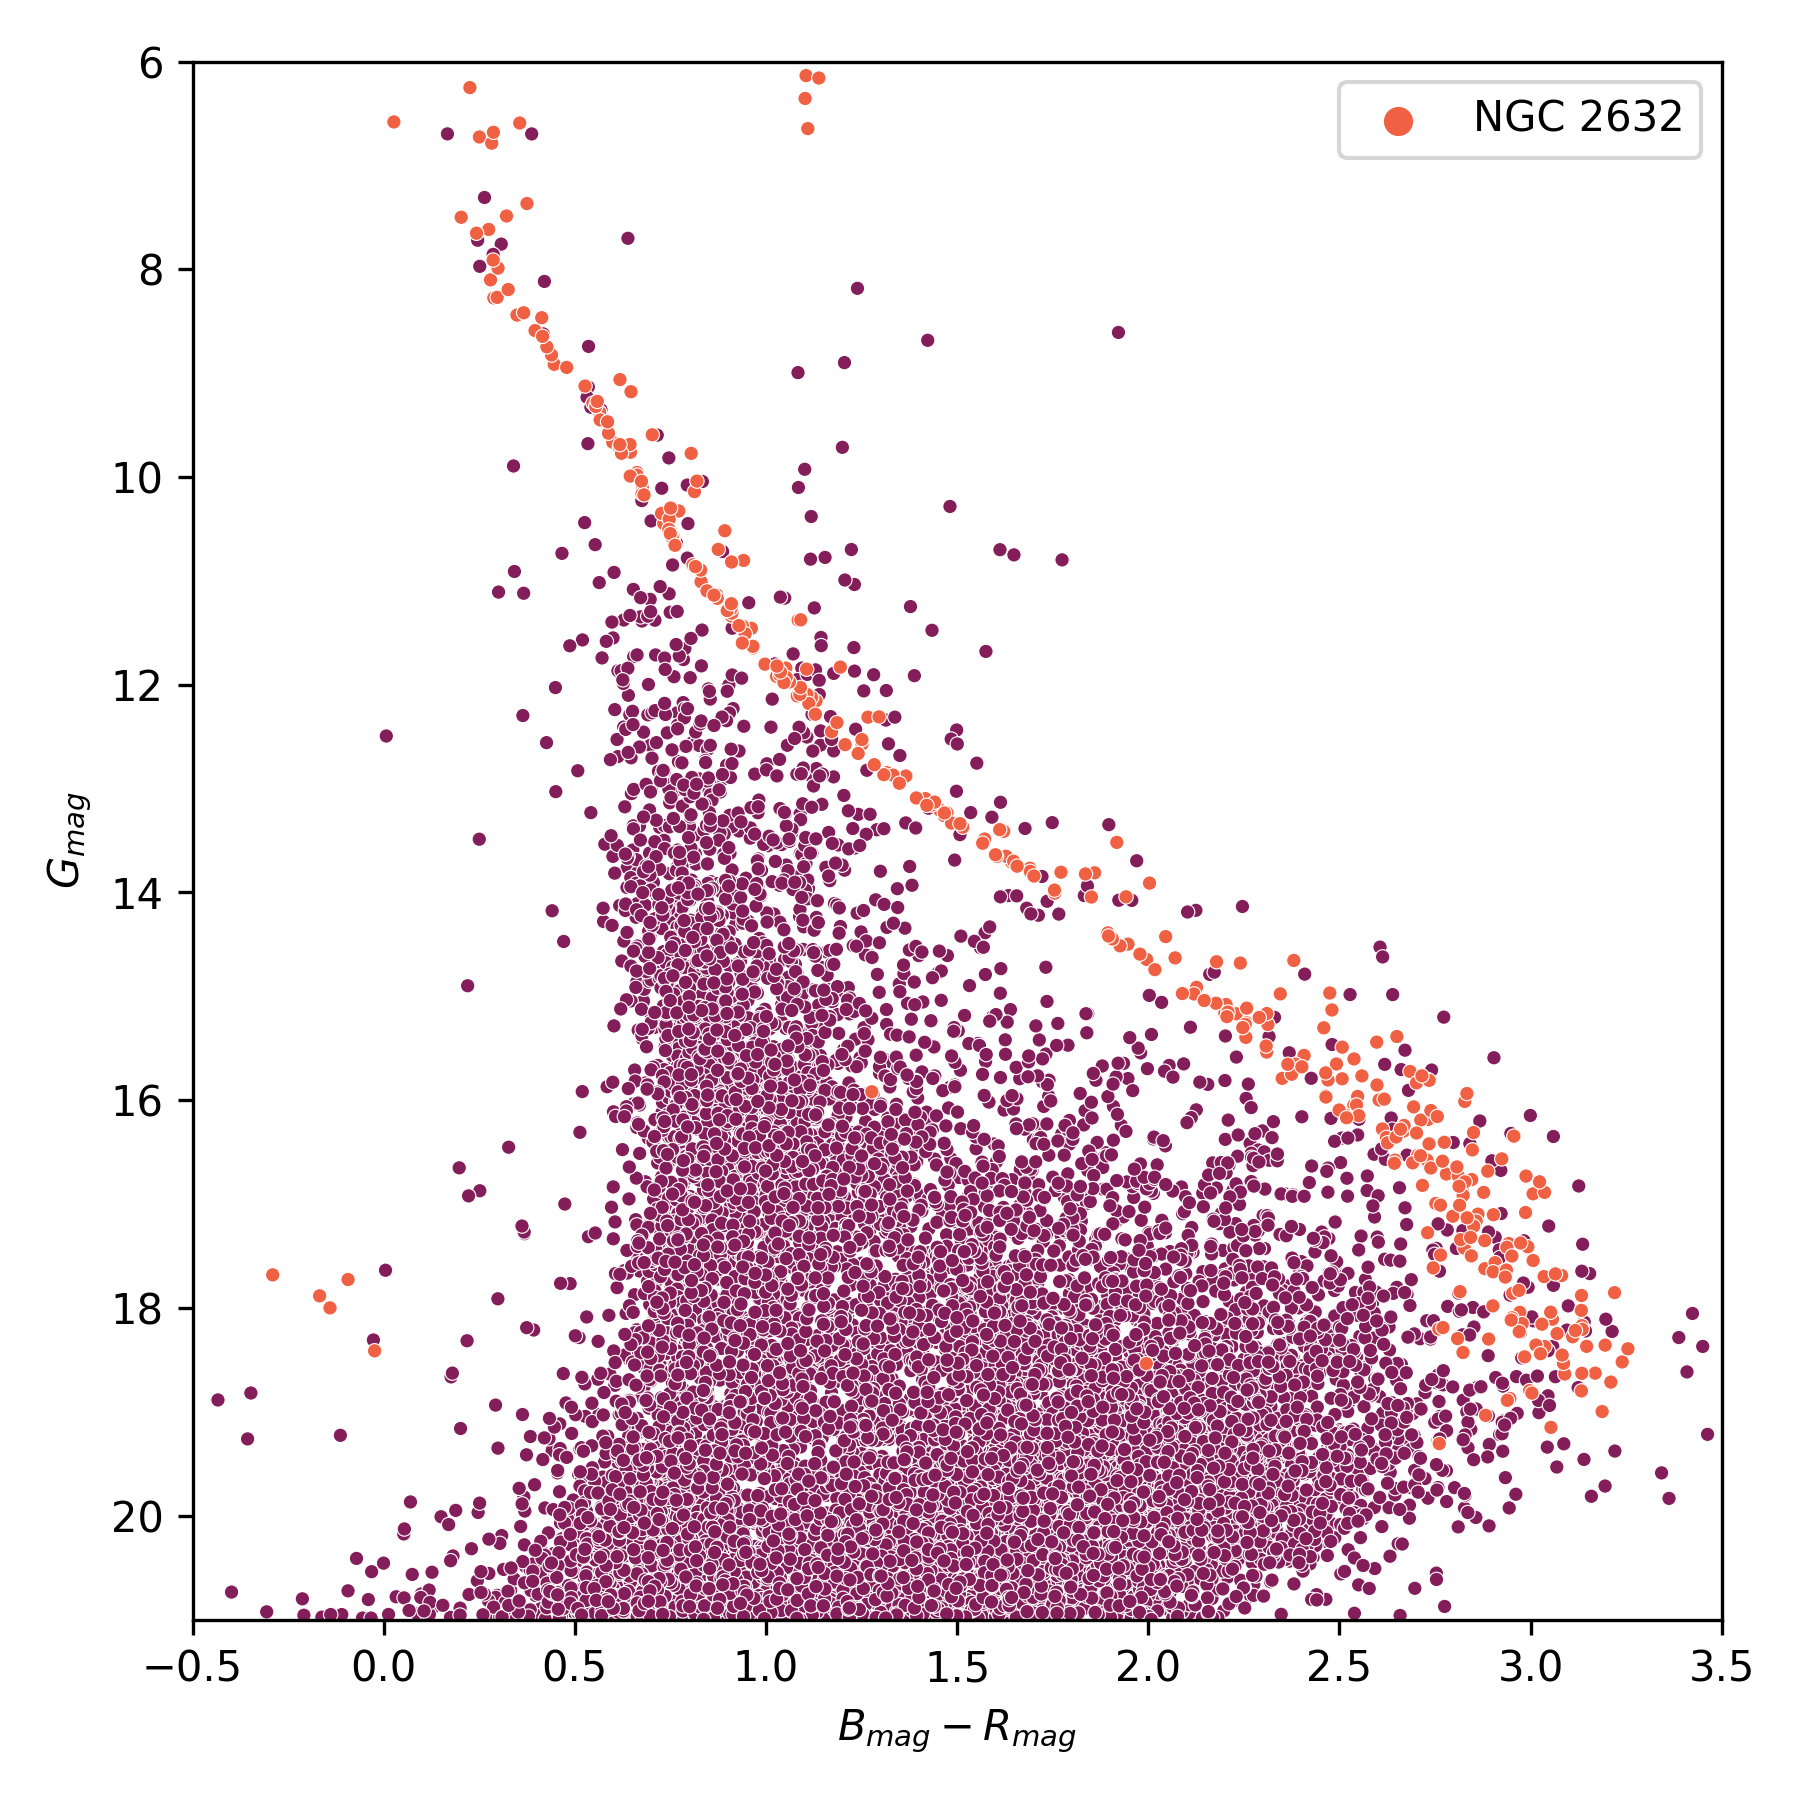
\includegraphics[width=\textwidth]{../figures/ngc_2632/hr_diagram_ngc_2632.png}
    \end{subfigure}
  \end{subfigure}
  \centering
  \begin{subfigure}{\columnwidth}
    \centering
    \begin{subfigure}[t]{0.30\textwidth}
      \centering
      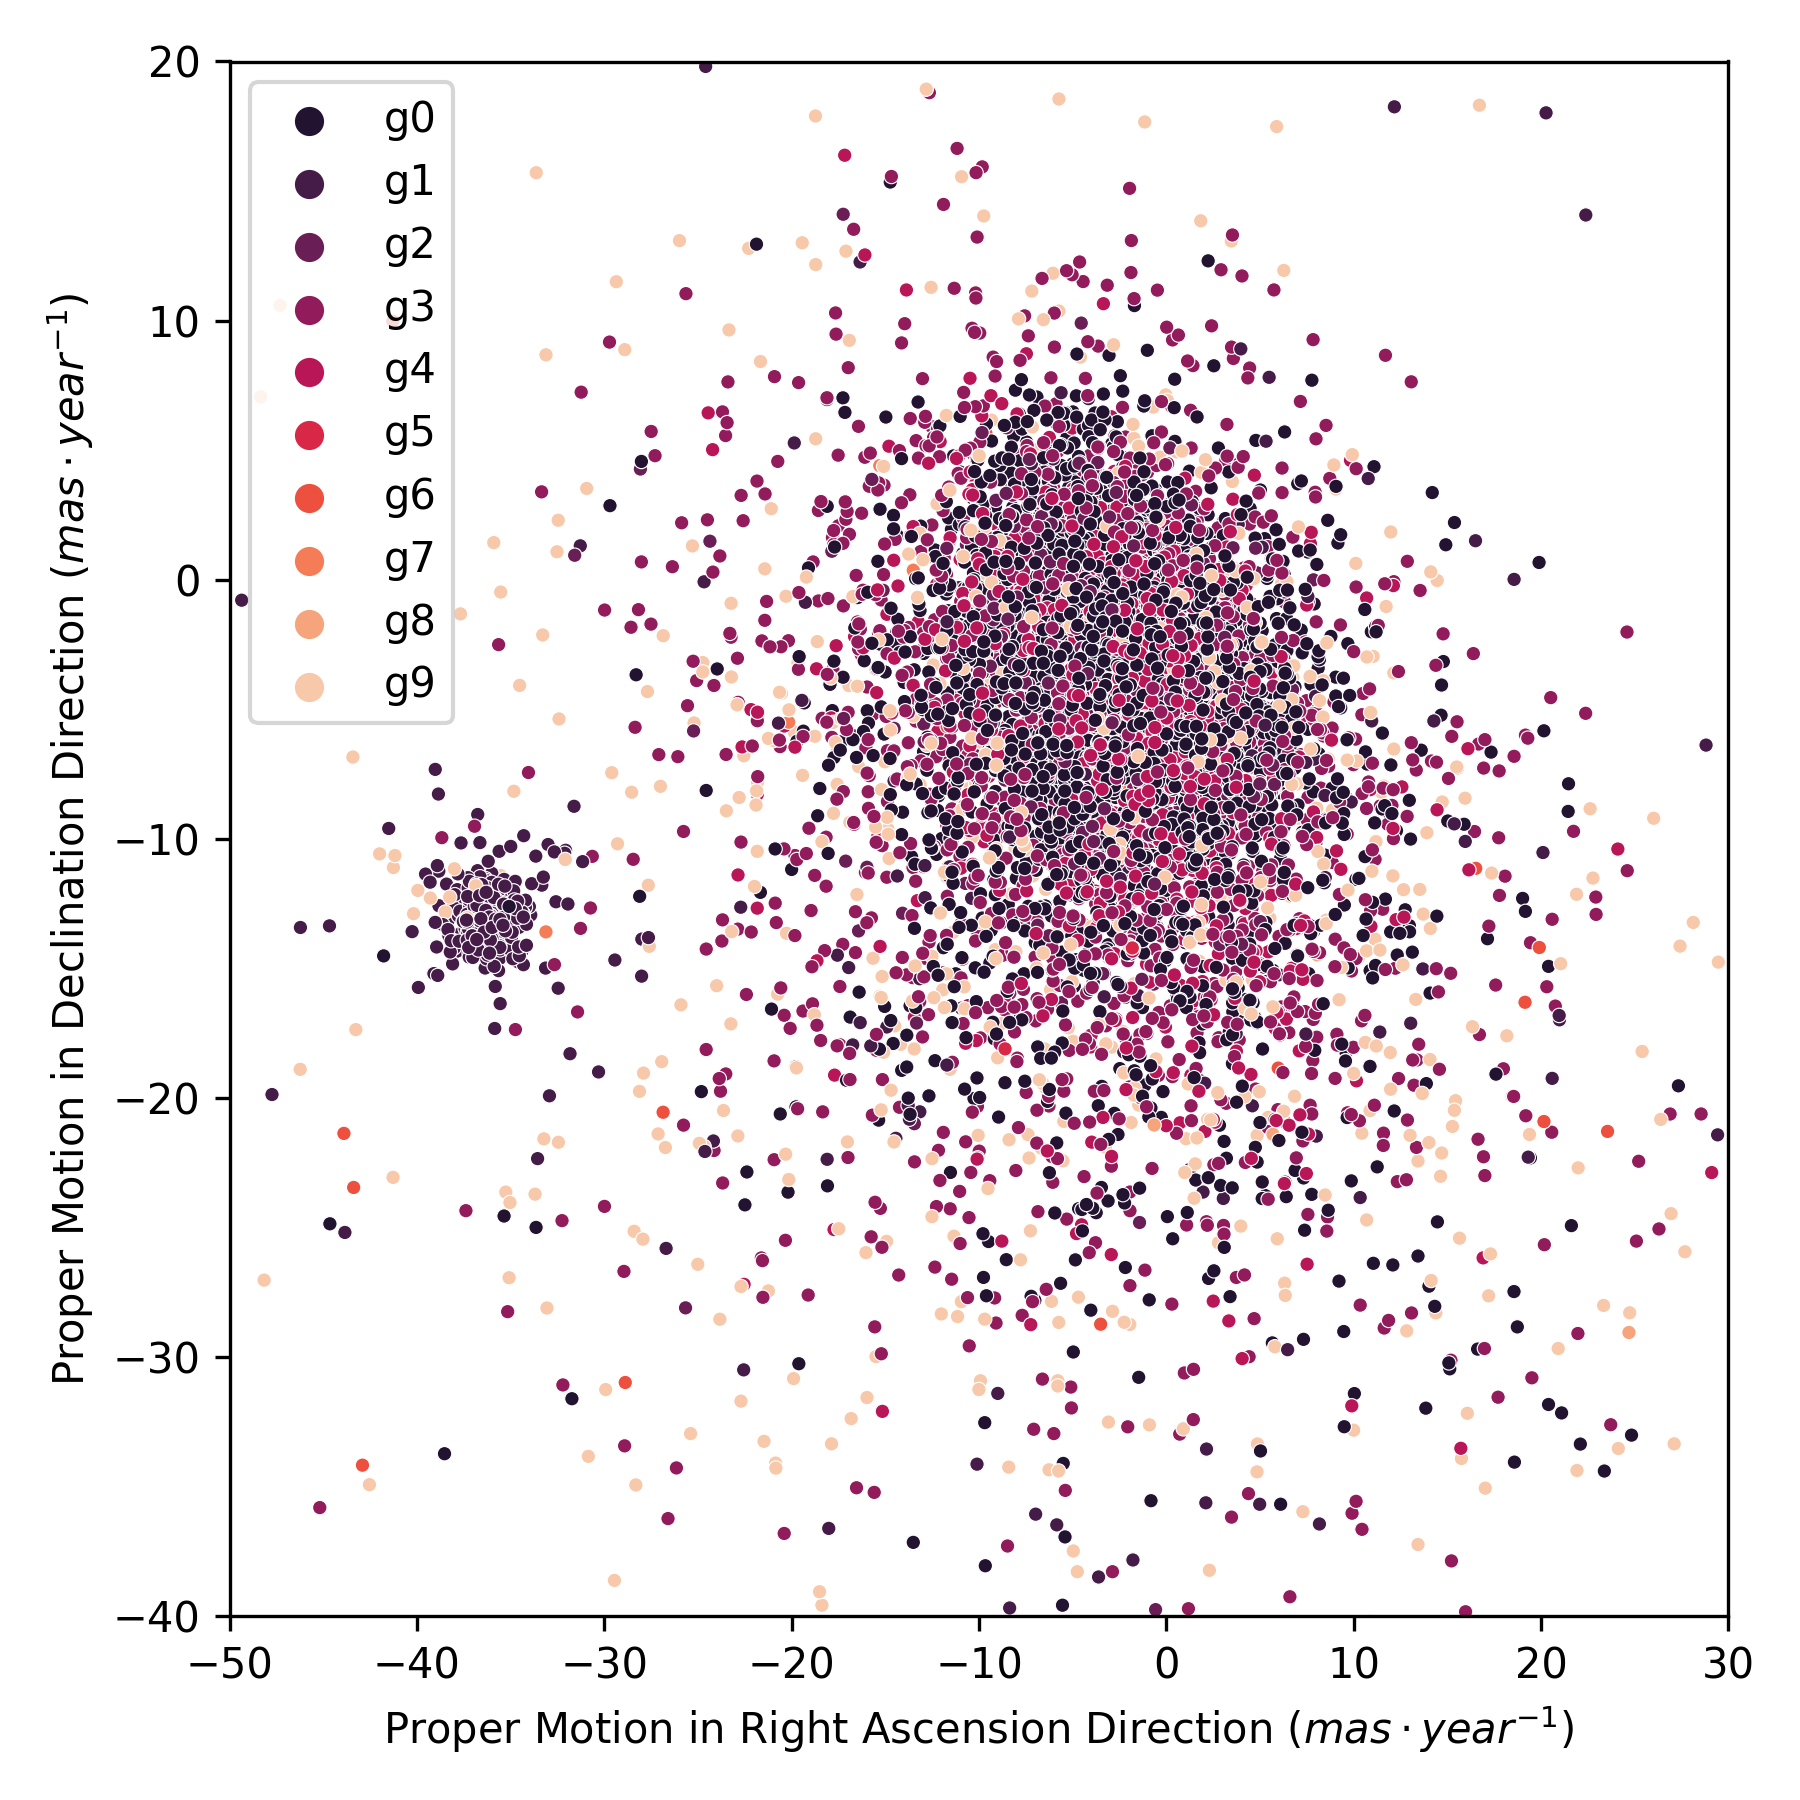
\includegraphics[width=\textwidth]{../figures/ngc_2632/kmeans_pm_ngc_2632.png}
    \end{subfigure}
    \hfill
    \begin{subfigure}[t]{0.30\textwidth}
      \centering
      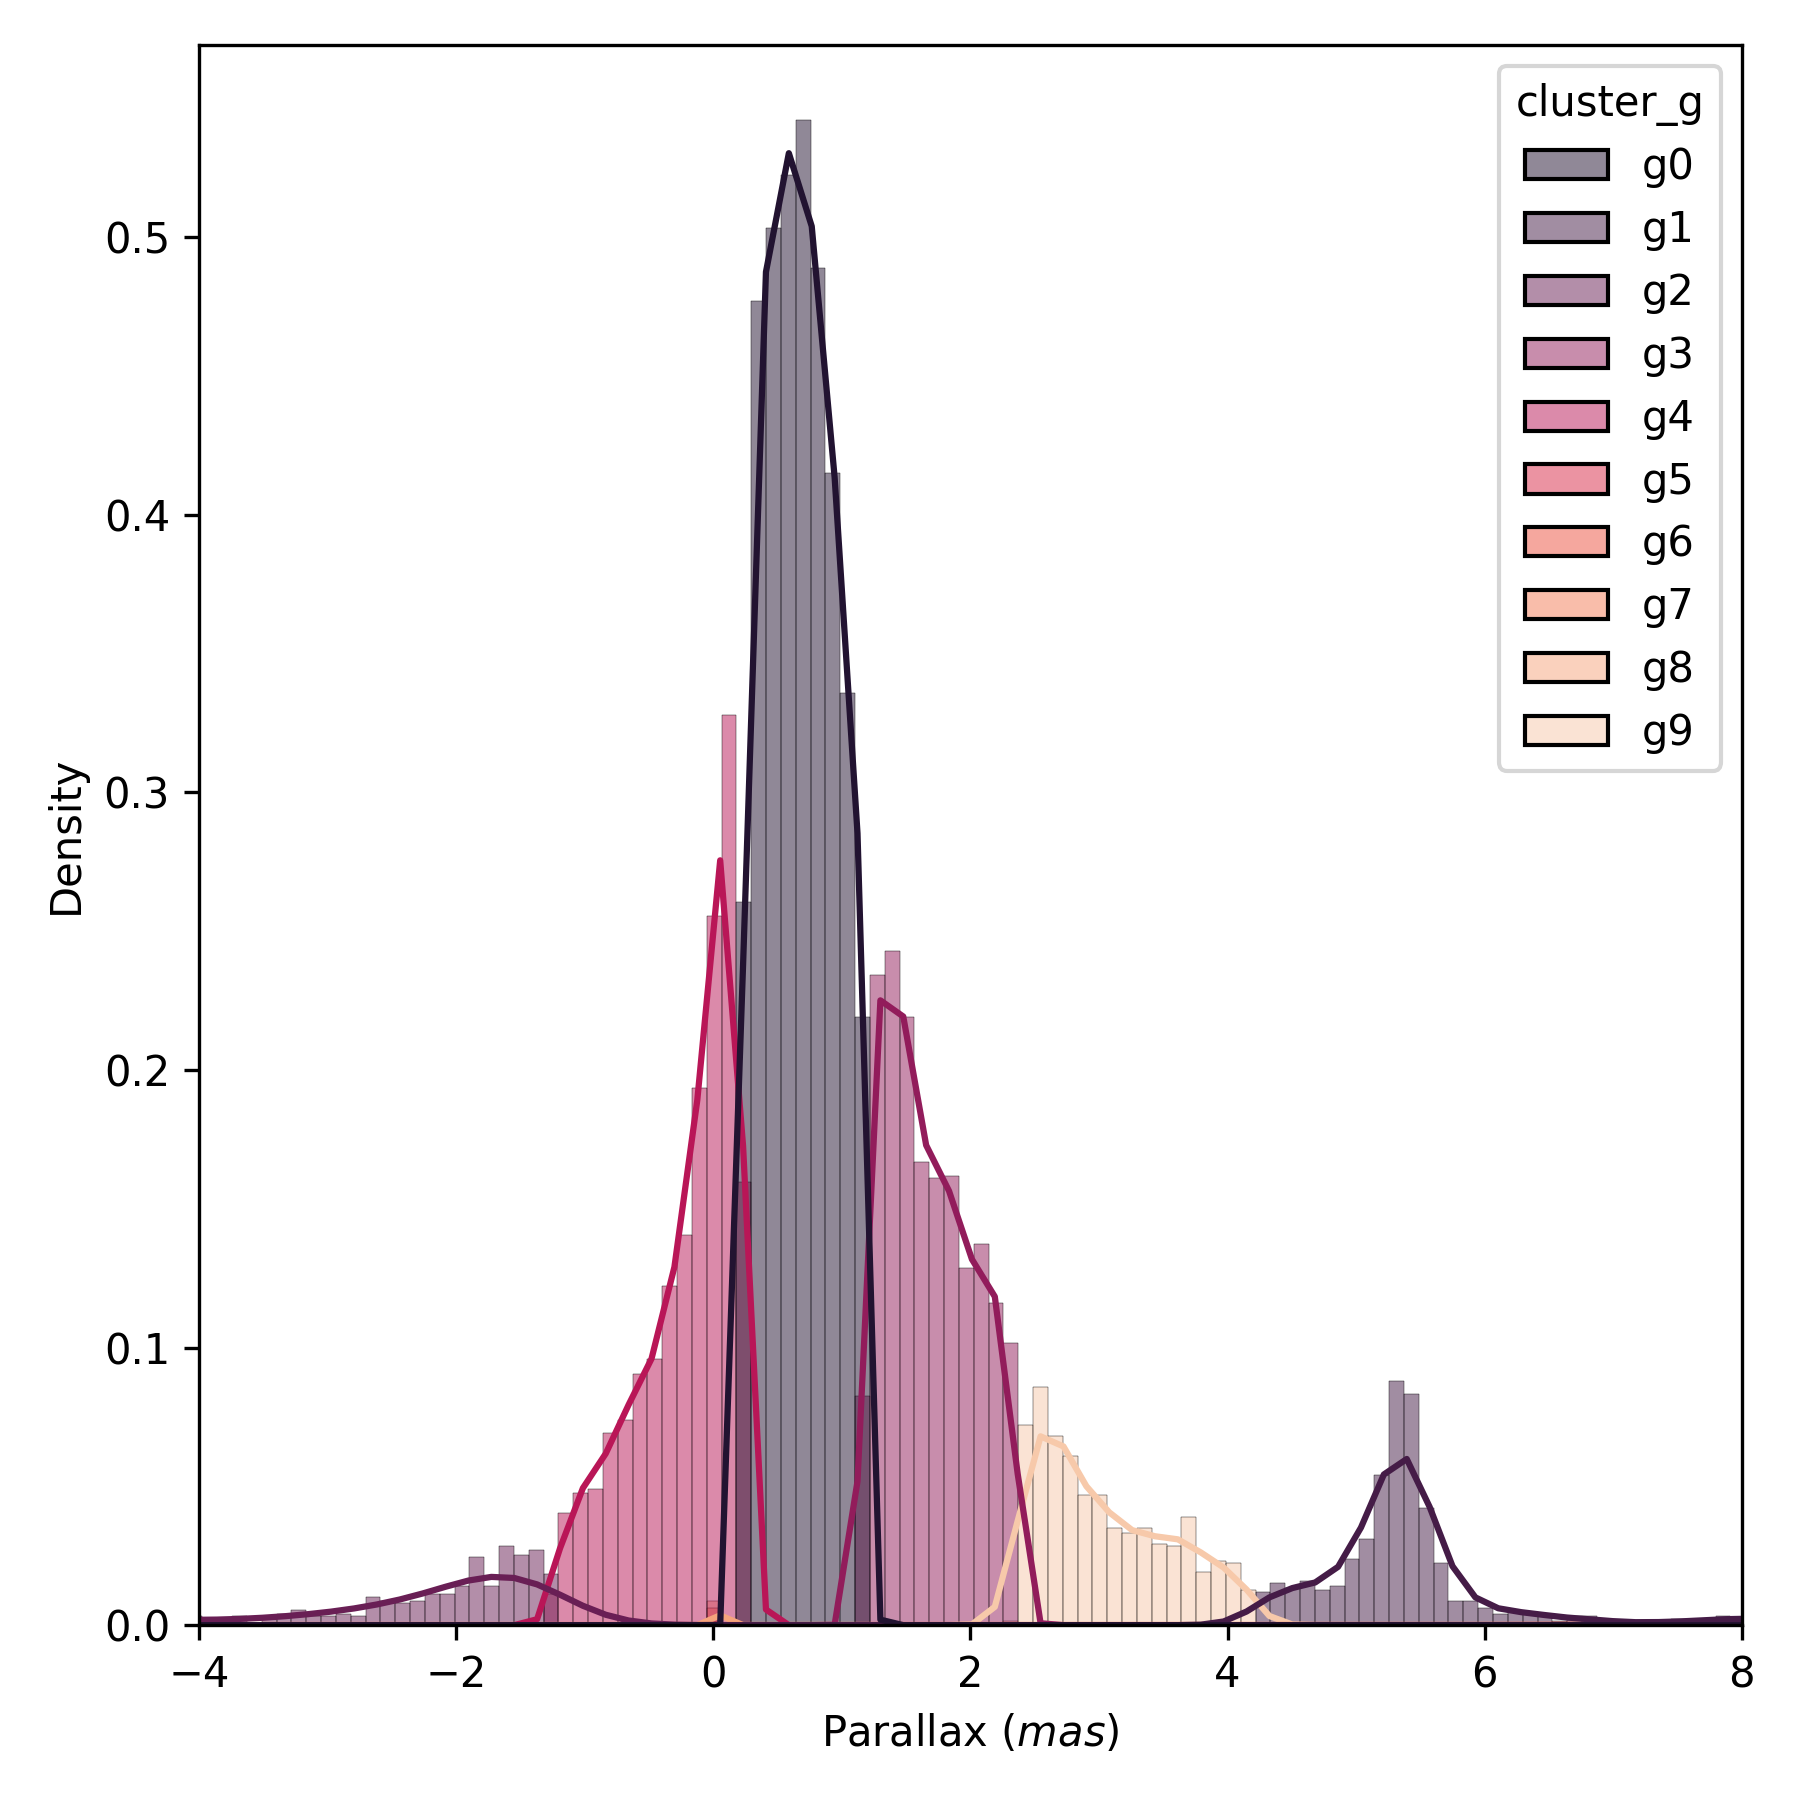
\includegraphics[width=\textwidth]{../figures/ngc_2632/kmeans_parallax_ngc_2632.png}
    \end{subfigure}
    \hfill
    \begin{subfigure}[t]{0.30\textwidth}
      \centering
      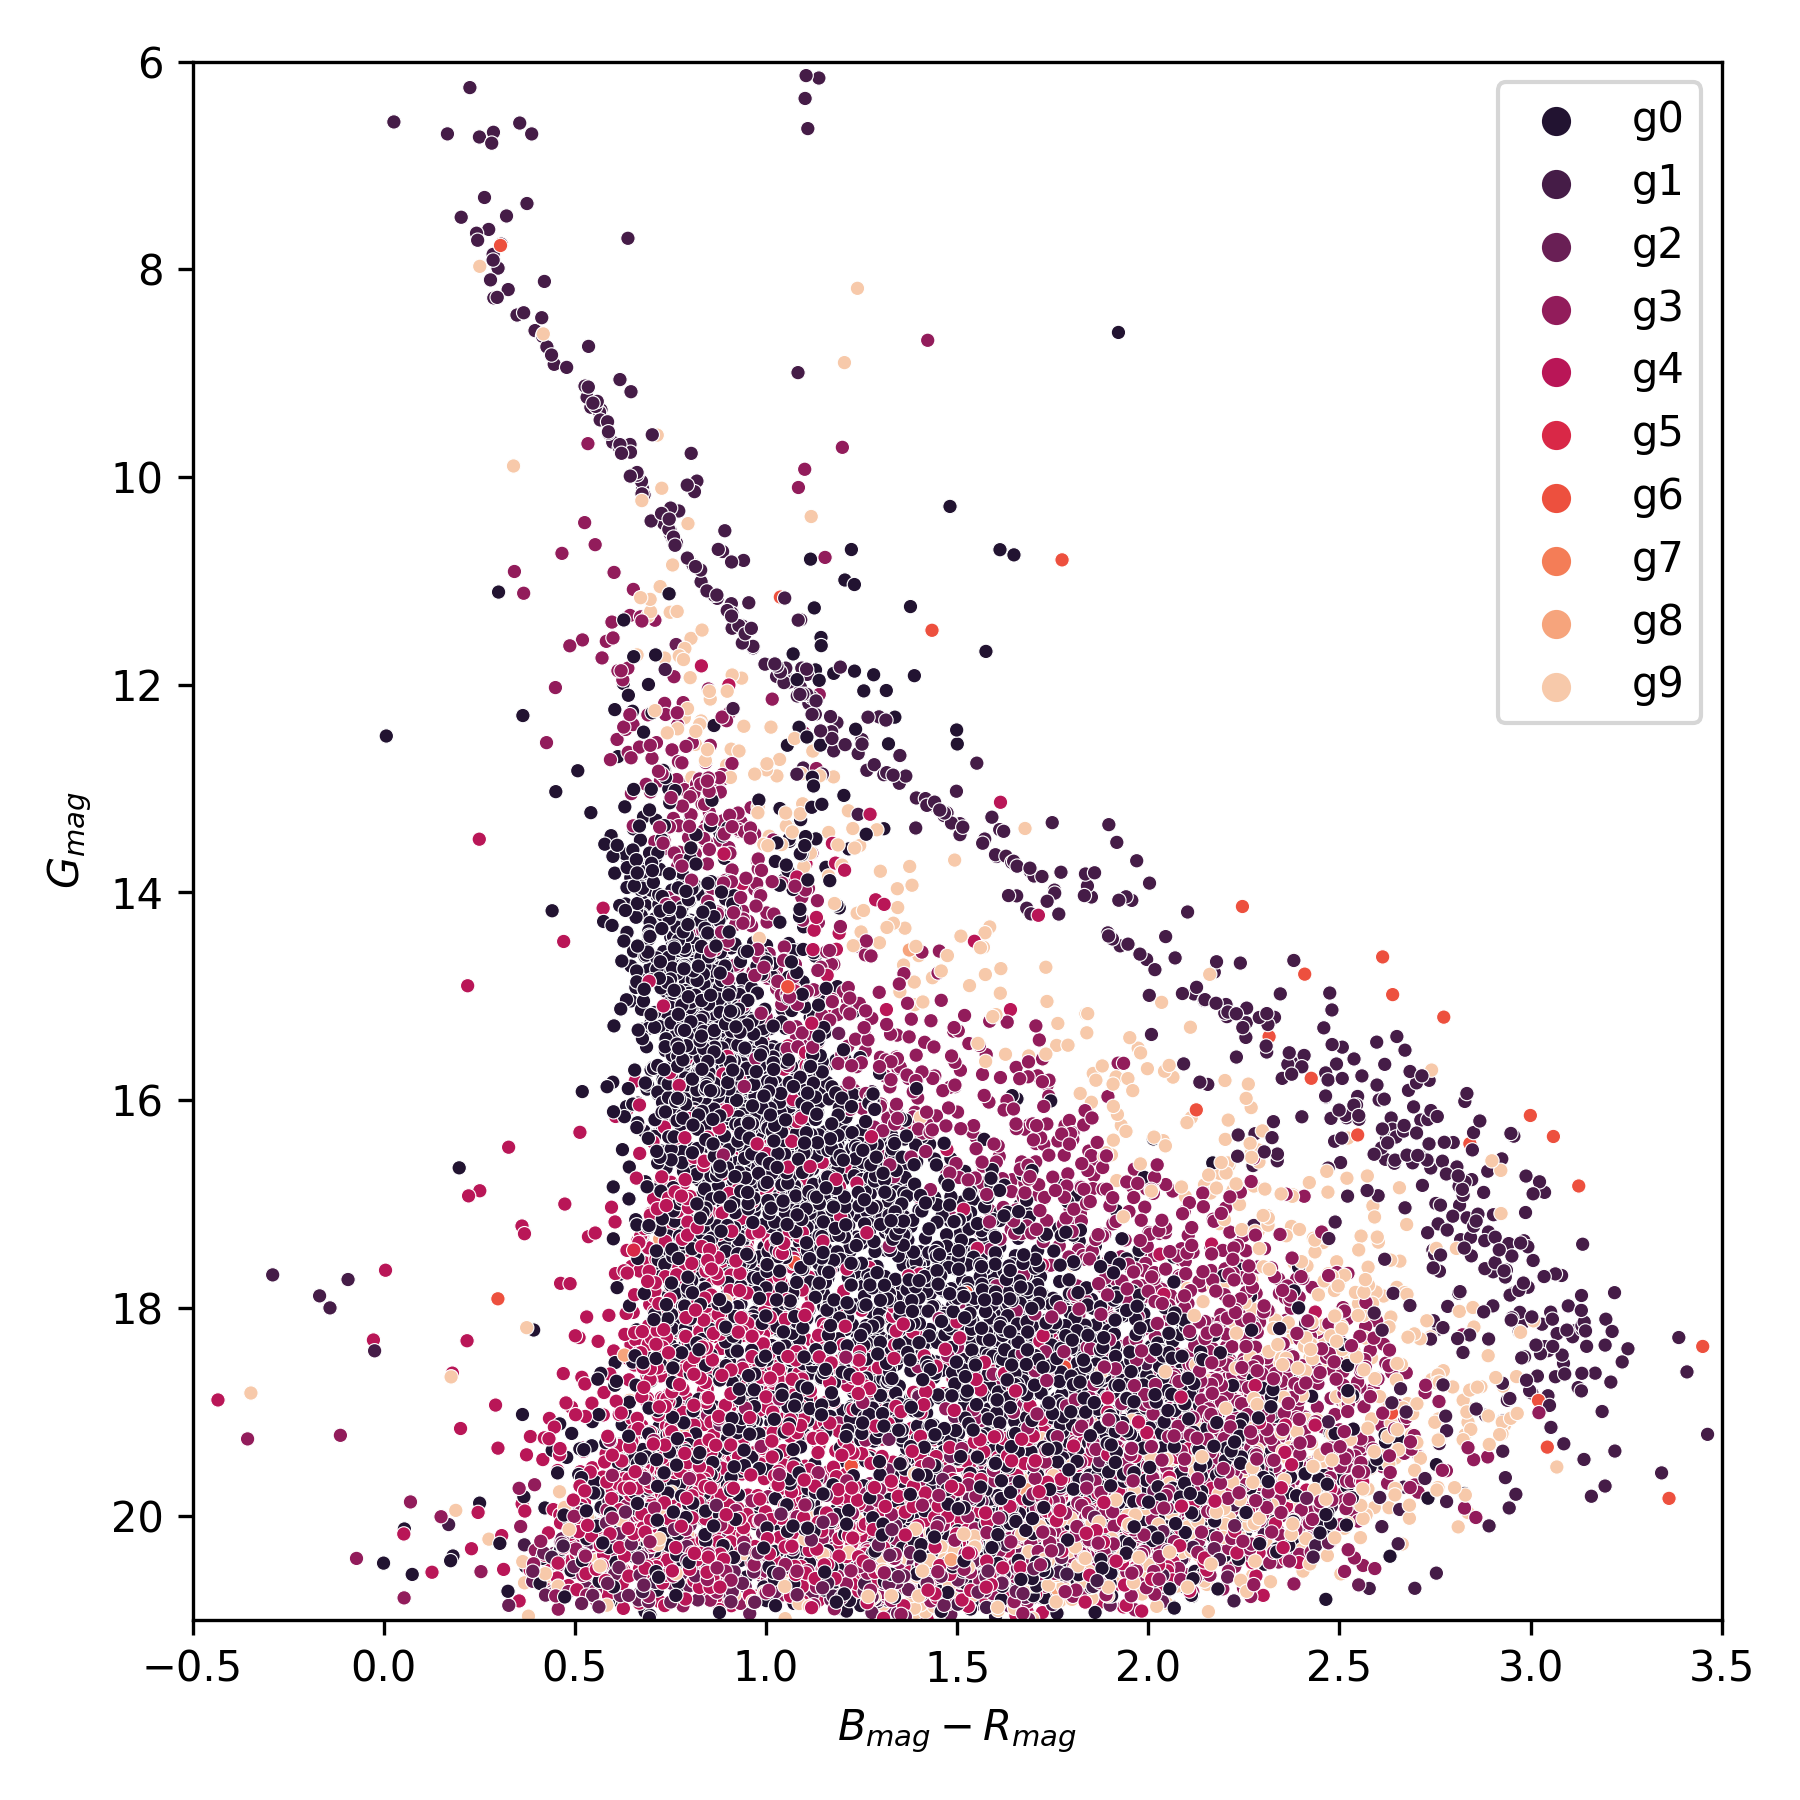
\includegraphics[width=\textwidth]{../figures/ngc_2632/kmeans_hr_diagram_ngc_2632.png}
    \end{subfigure}
  \end{subfigure}
  \caption{NGC 2632 characterization using Clusterix+TOPCAT (top) and K-Means (bottom).
           K-Means identifies NGC 2632 as \emph{g1}.}
  \label{fig:app_result_ngc_2632_clusterix_kmeans}
\end{figure}

Figure~\ref{fig:app_result_ngc_2632_dec} shows the groups found using
the DEC model (first row) and the DEC model filtered (second row).
Open cluster NGC 2632 is labeled as group \emph{g1}.

\begin{figure}[htbp]
  \centering
  \begin{subfigure}{\columnwidth}
    \centering
    \begin{subfigure}[t]{0.30\textwidth}
      \centering
      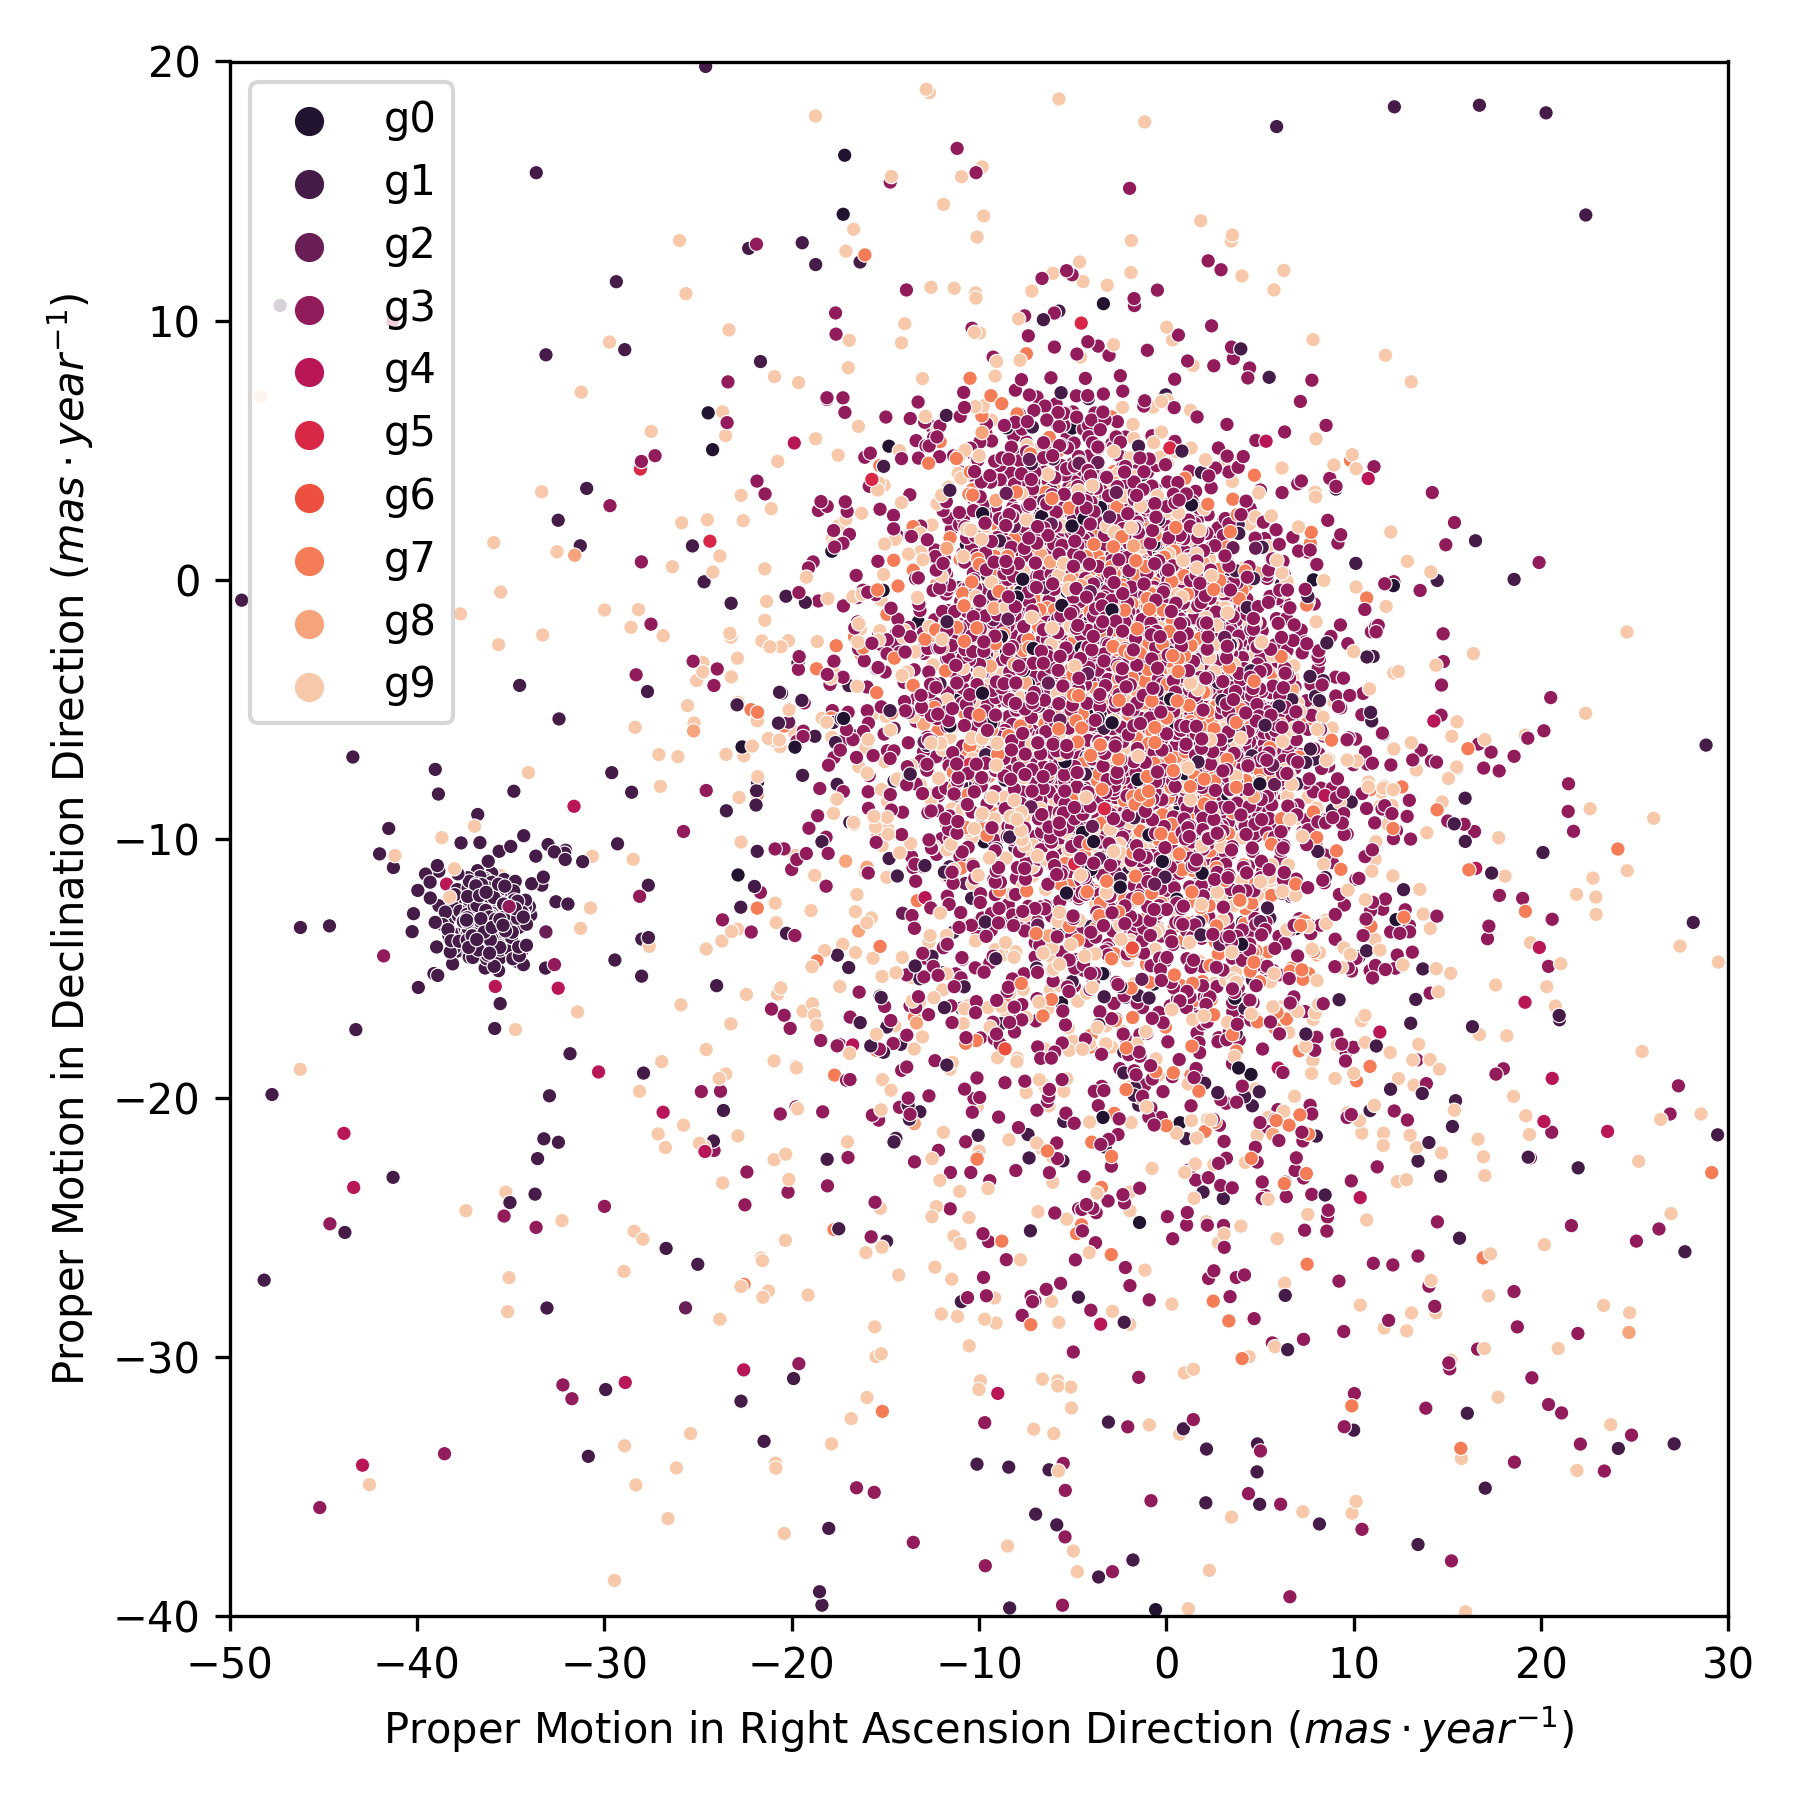
\includegraphics[width=\textwidth]{../figures/ngc_2632/dec_pm_ngc_2632.png}
    \end{subfigure}
    \hfill
    \begin{subfigure}[t]{0.30\textwidth}
      \centering
      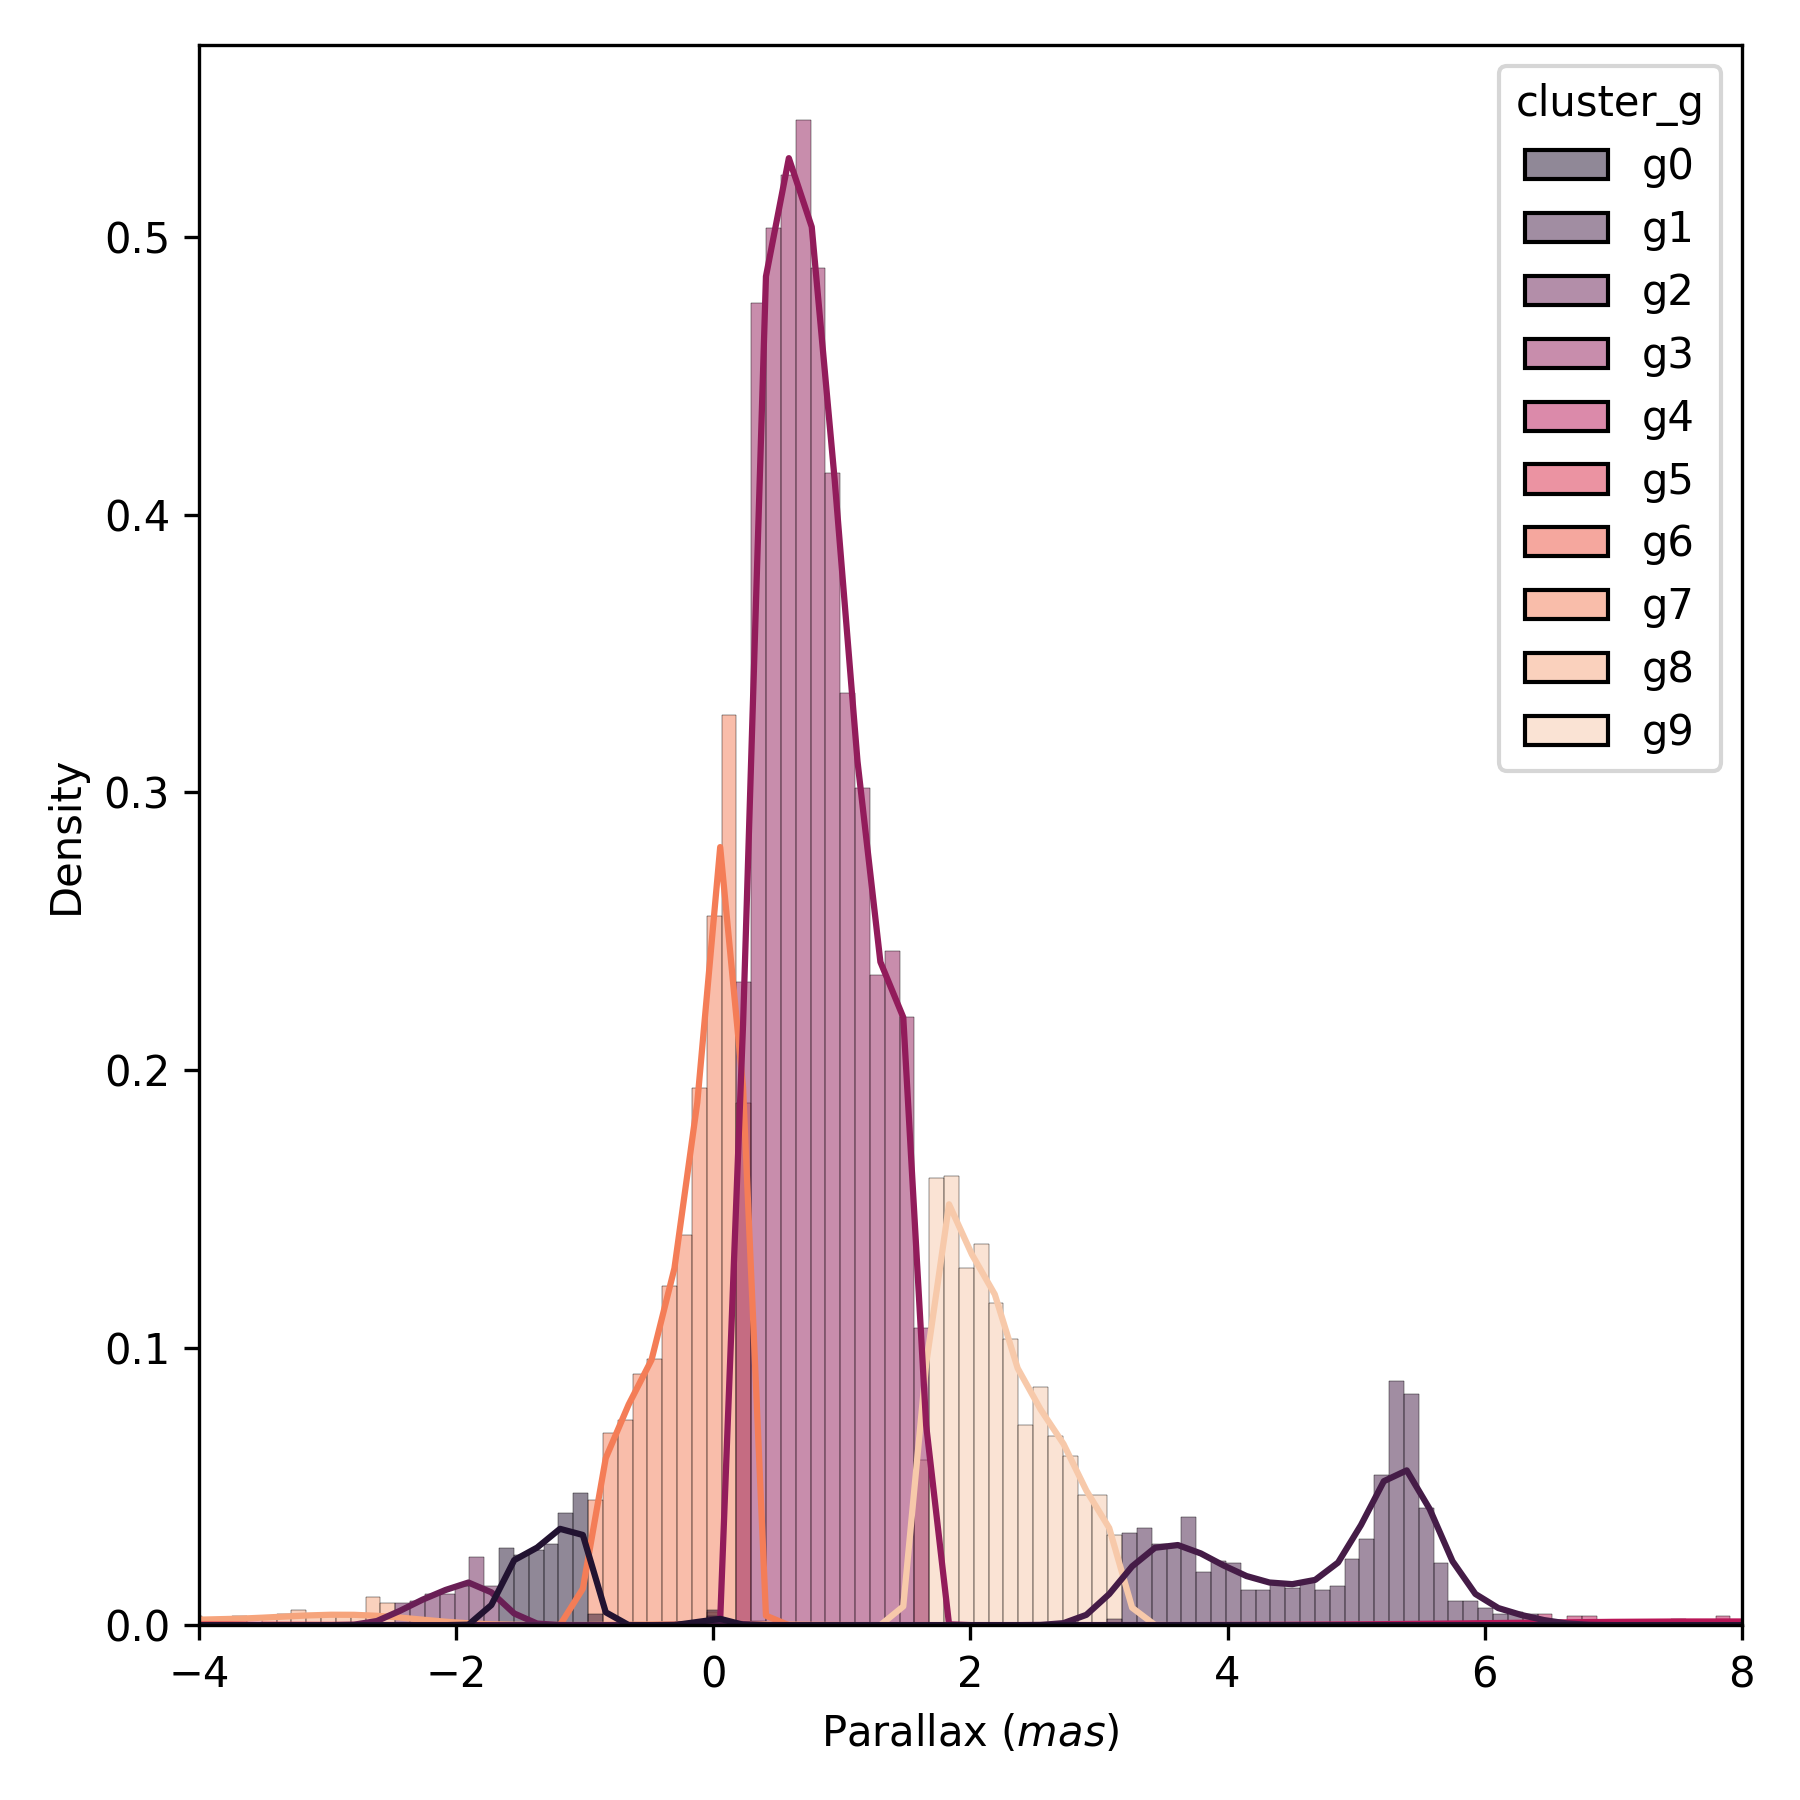
\includegraphics[width=\textwidth]{../figures/ngc_2632/dec_parallax_ngc_2632.png}
    \end{subfigure}
    \hfill
    \begin{subfigure}[t]{0.30\textwidth}
      \centering
      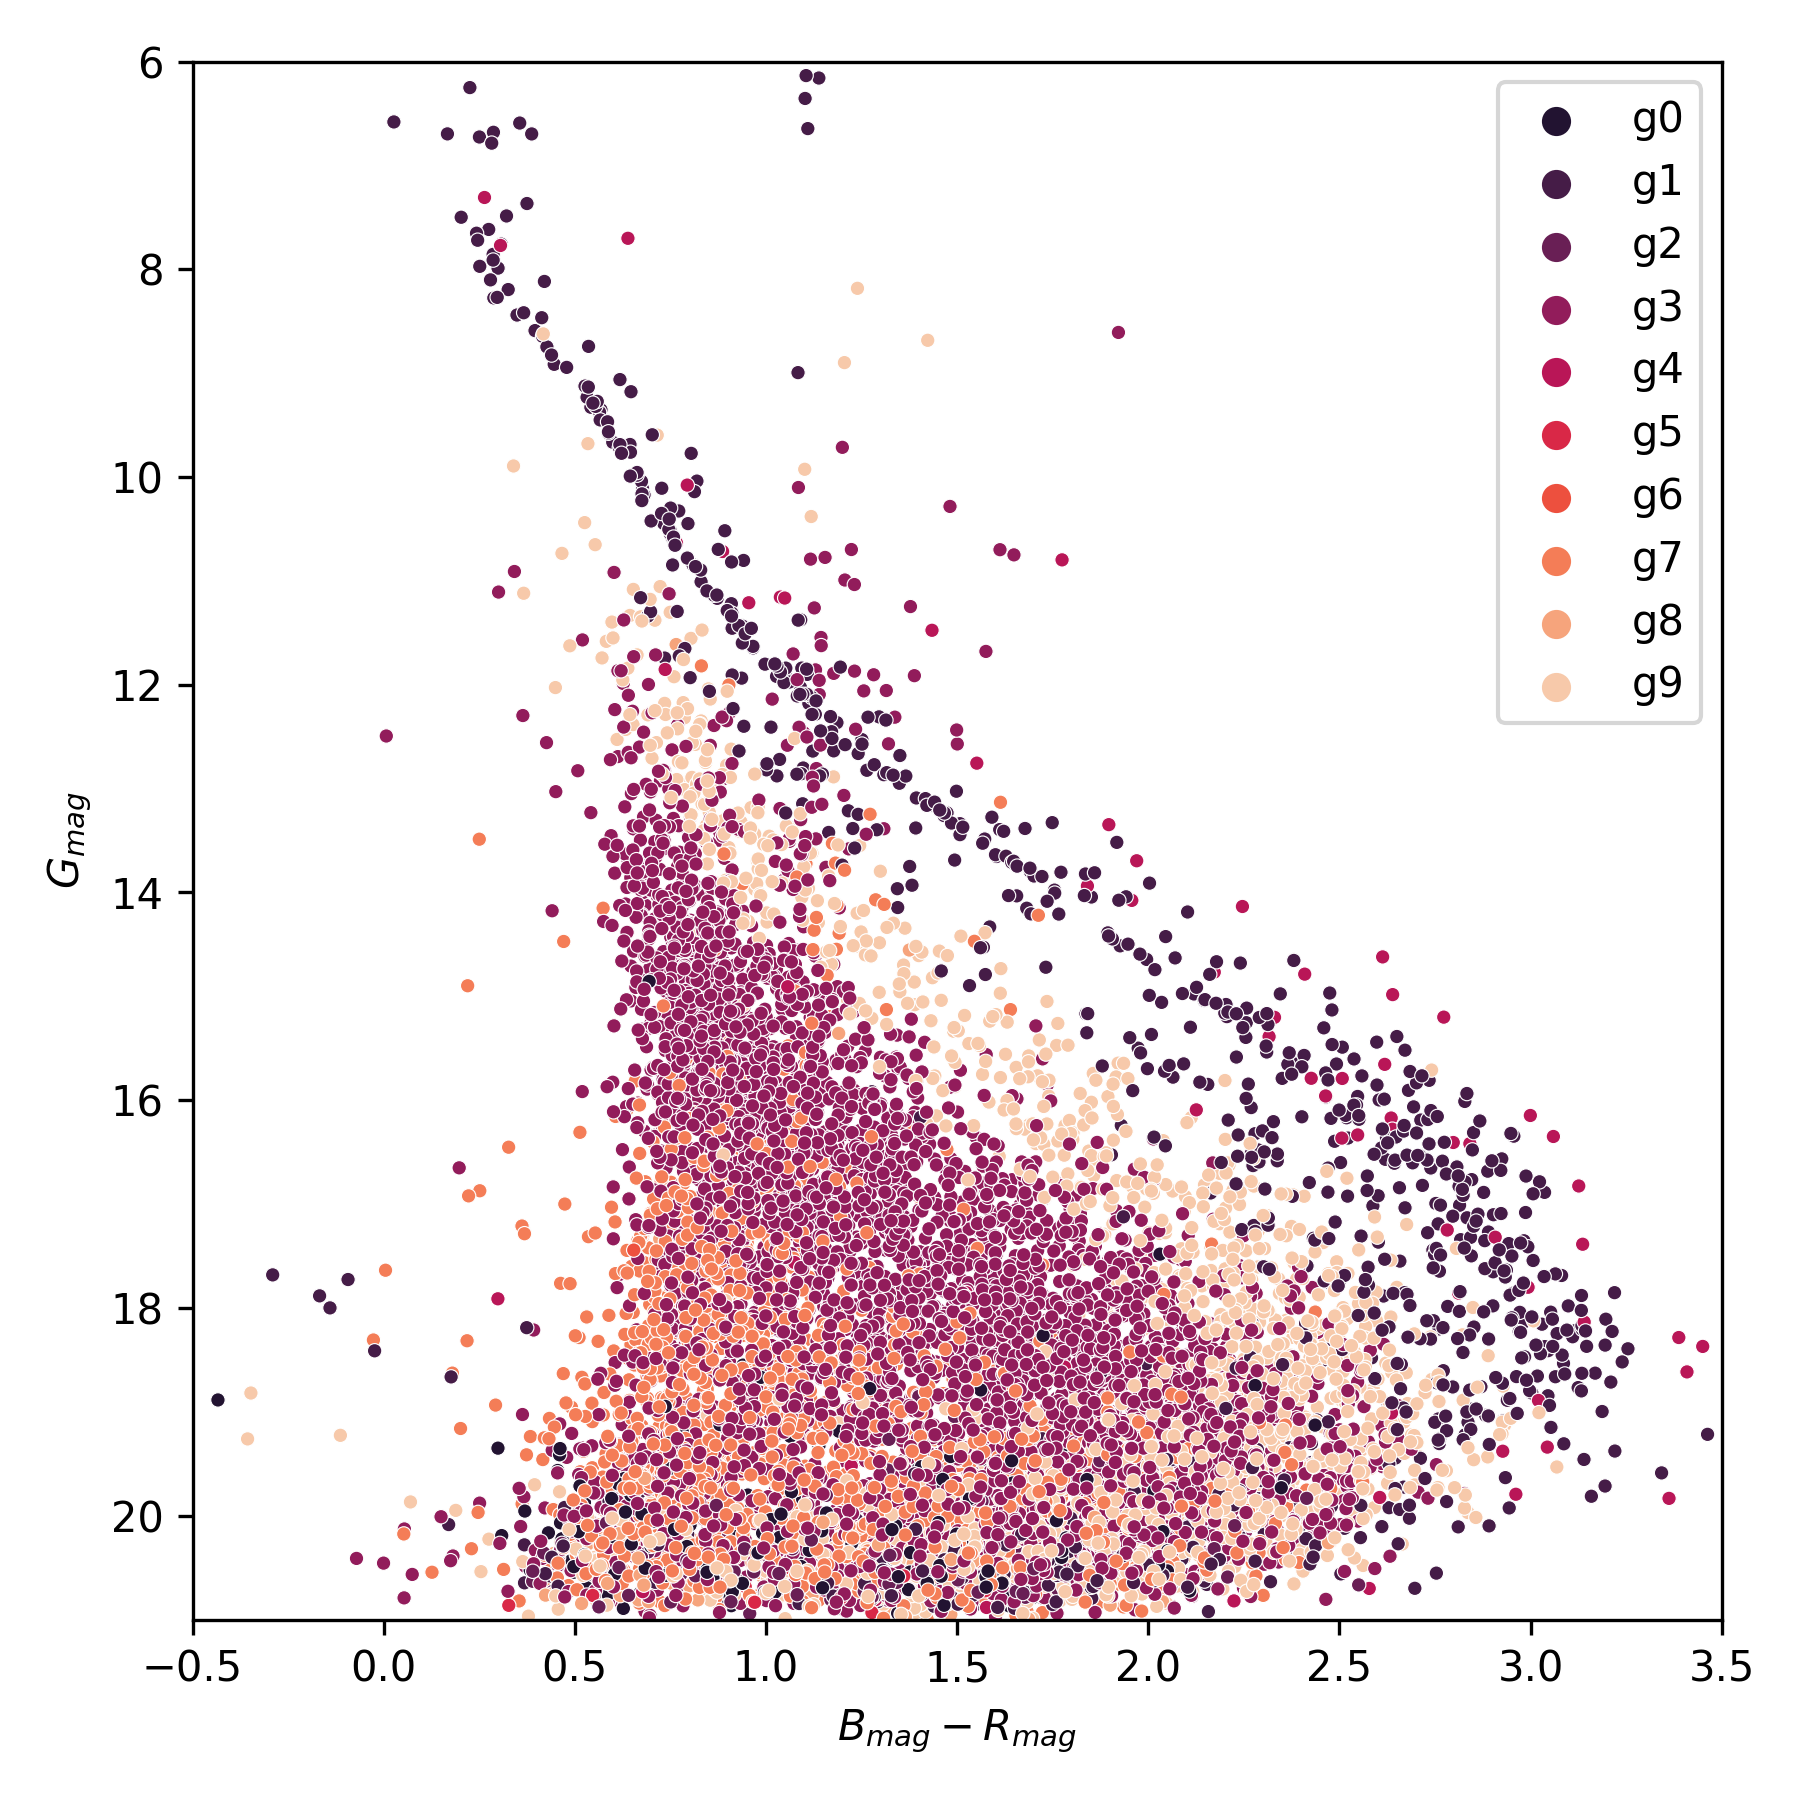
\includegraphics[width=\textwidth]{../figures/ngc_2632/dec_hr_diagram_ngc_2632.png}
    \end{subfigure}
  \end{subfigure}
  \centering
  \begin{subfigure}{\columnwidth}
    \centering
    \begin{subfigure}[t]{0.30\textwidth}
      \centering
      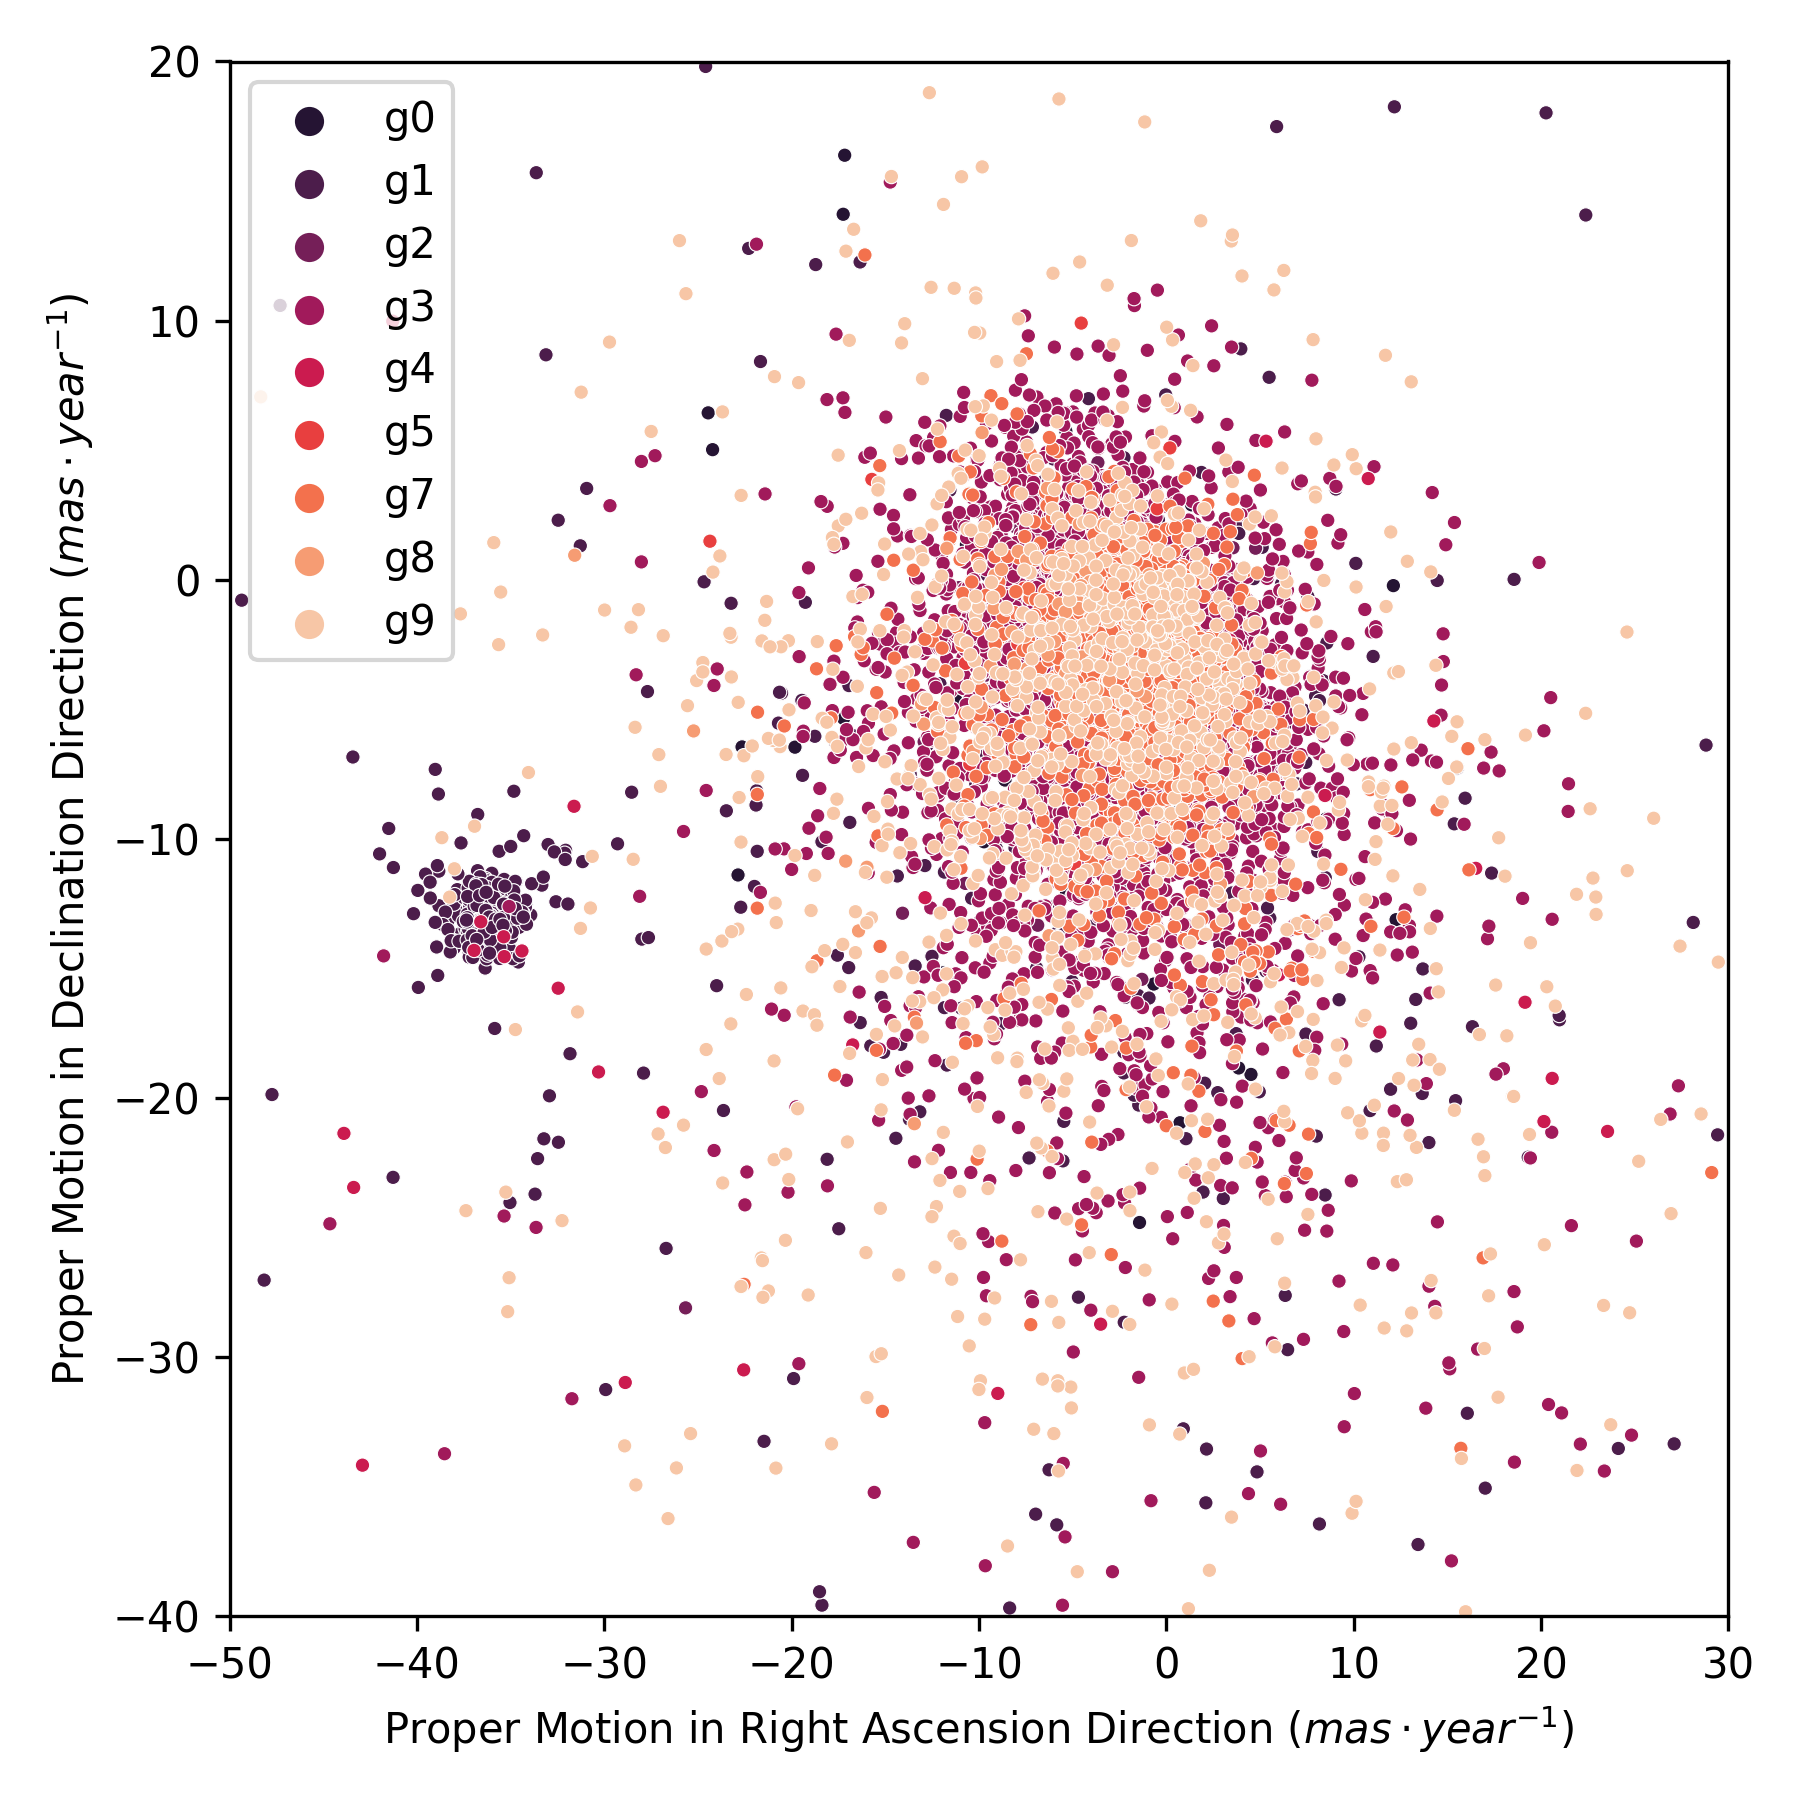
\includegraphics[width=\textwidth]{../figures/ngc_2632/dec_pm_filtered_ngc_2632.png}
    \end{subfigure}
    \hfill
    \begin{subfigure}[t]{0.30\textwidth}
      \centering
      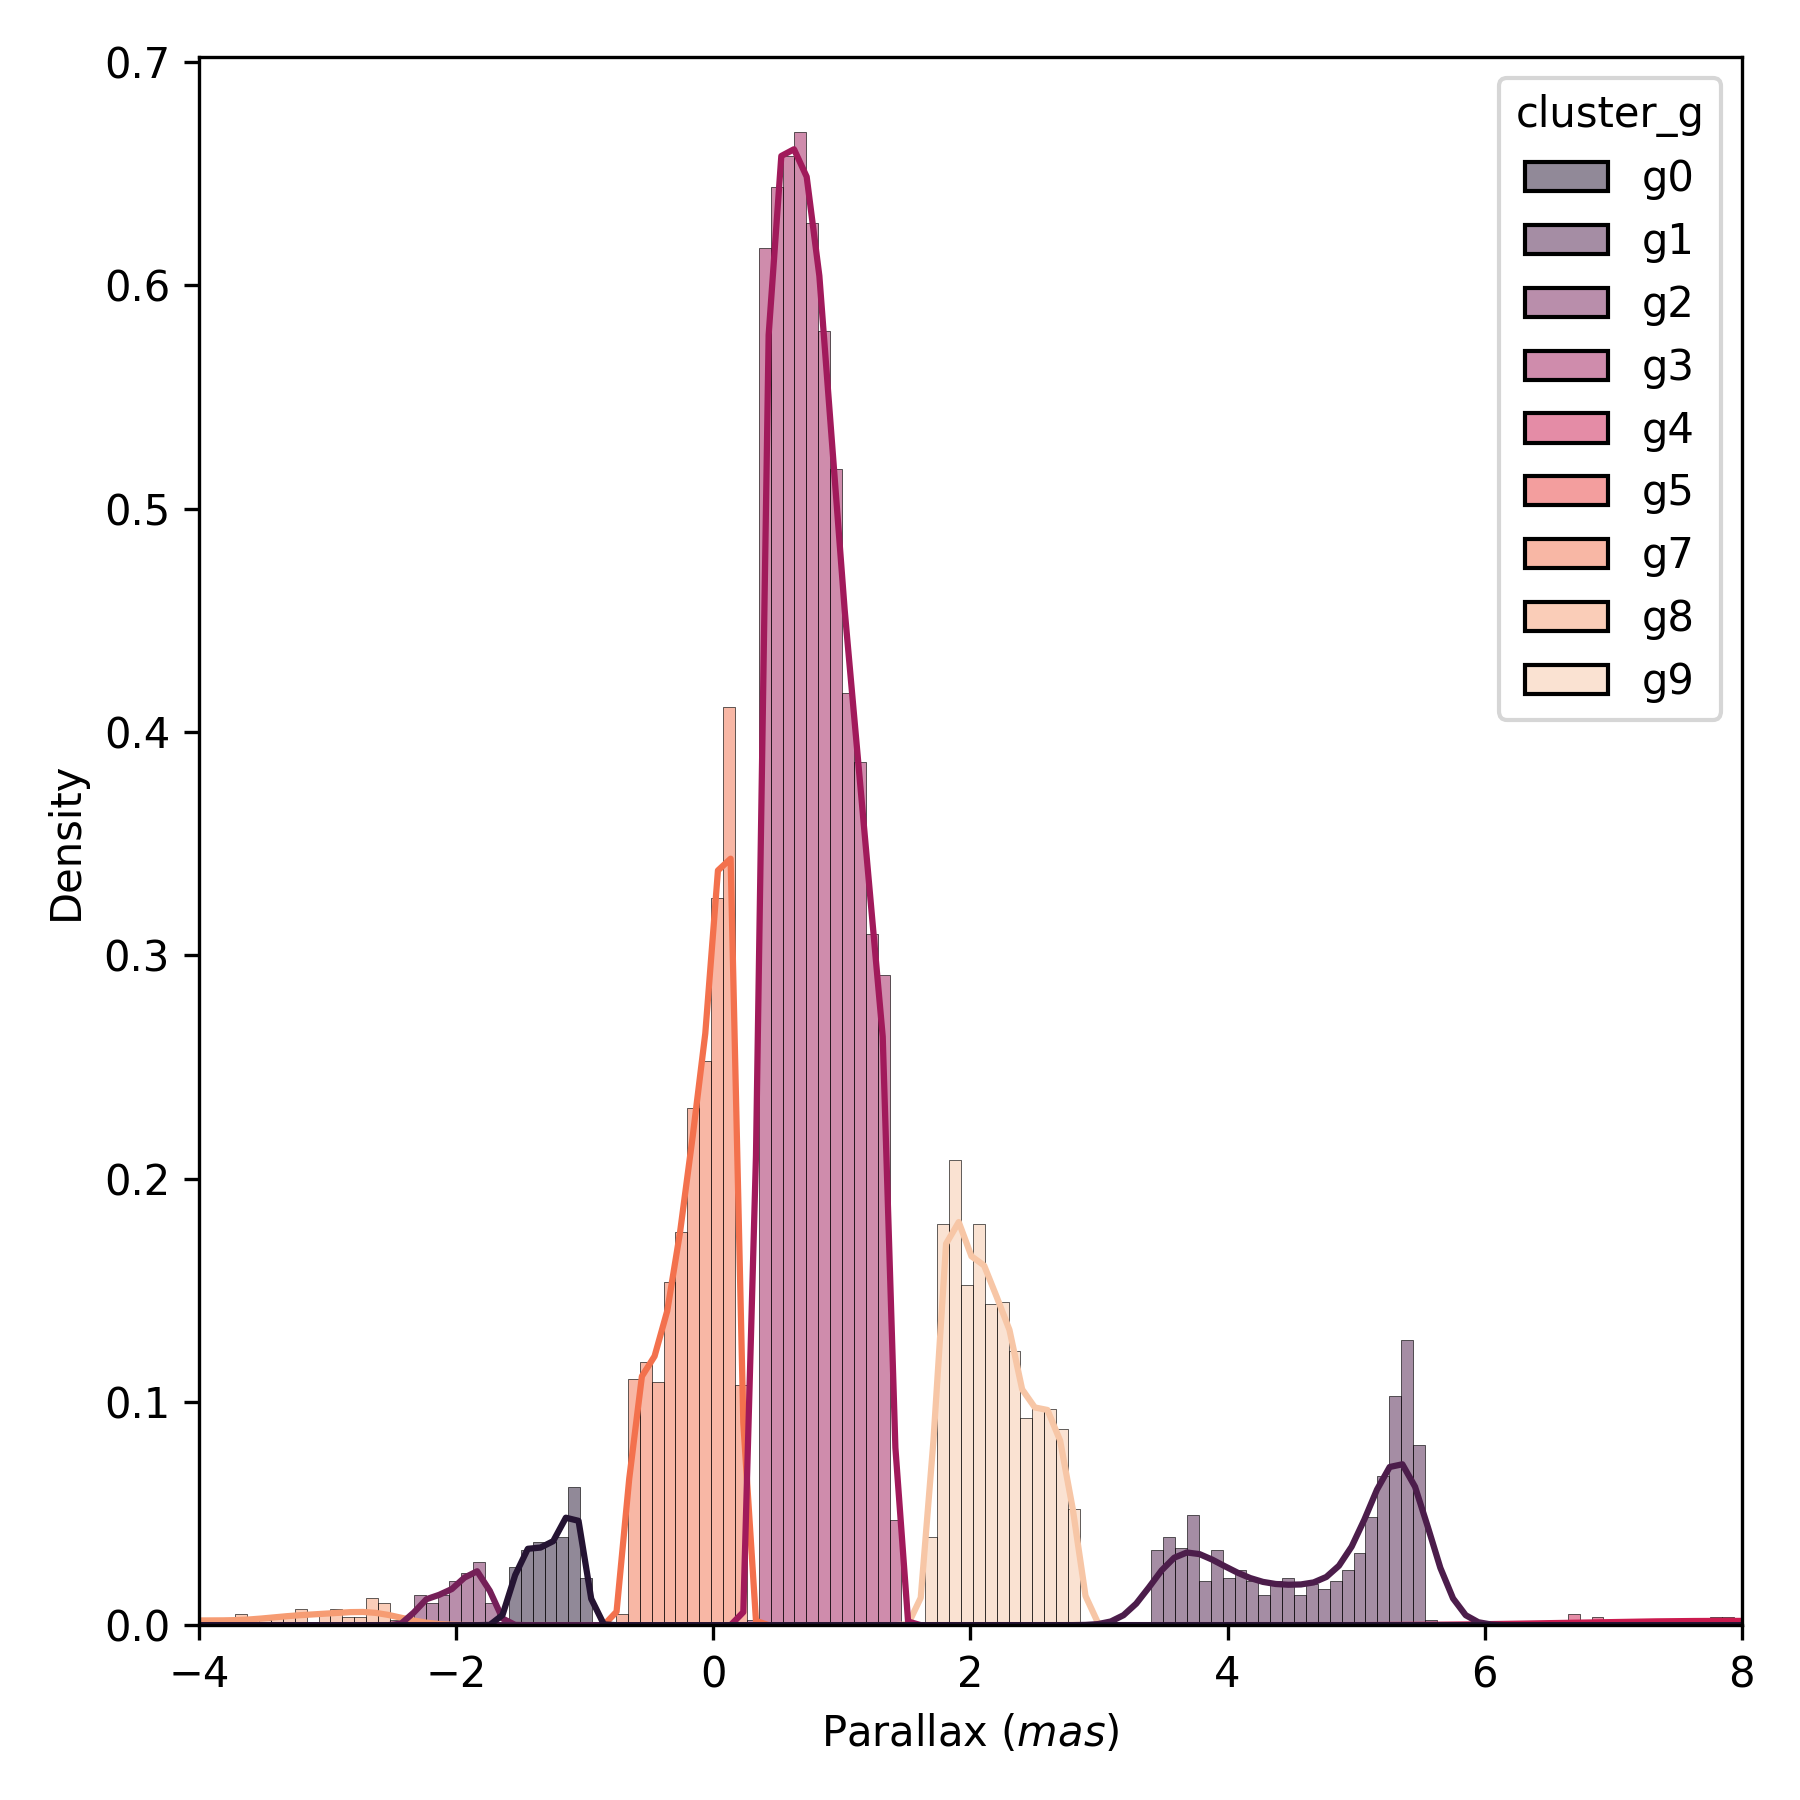
\includegraphics[width=\textwidth]{../figures/ngc_2632/dec_parallax_filtered_ngc_2632.png}
    \end{subfigure}
    \hfill
    \begin{subfigure}[t]{0.30\textwidth}
      \centering
      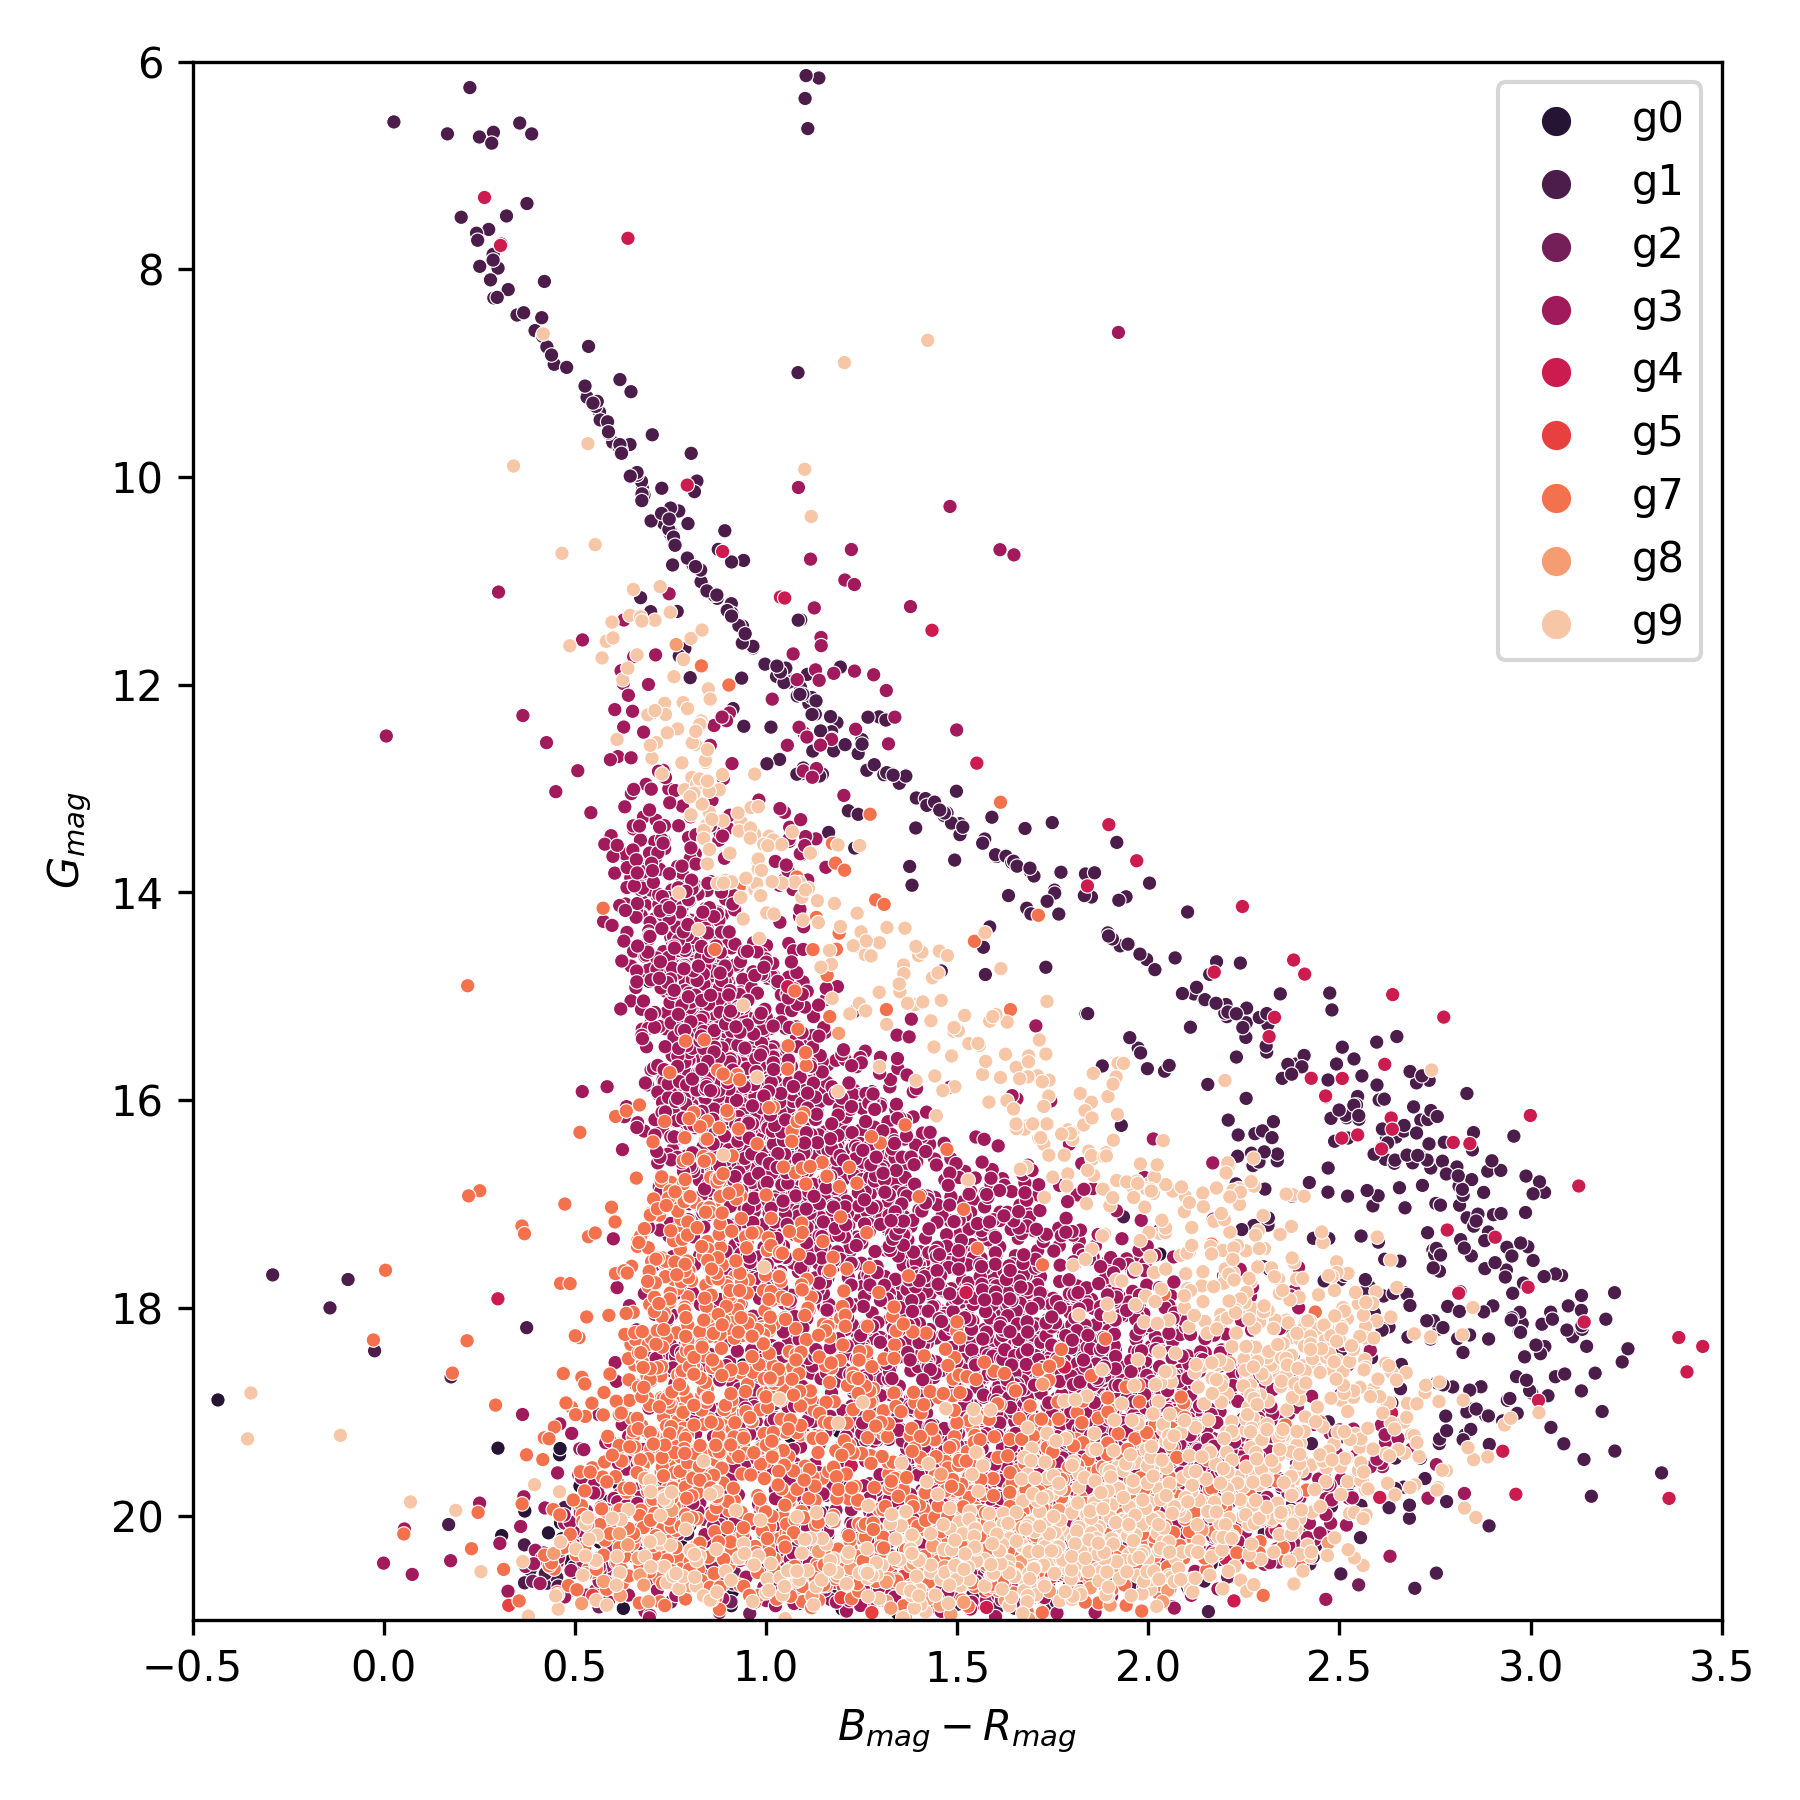
\includegraphics[width=\textwidth]{../figures/ngc_2632/dec_hr_diagram_filtered_ngc_2632.png}
    \end{subfigure}
  \end{subfigure}
  \caption{NGC 2632 characterization using DEC model (top) and DEC (filtered) (bottom).
           NGC 2632 is identified as \emph{g1}.}
  \label{fig:app_result_ngc_2632_dec}
\end{figure}

\begin{table}[htbp]
  \begin{center}
    \resizebox{\columnwidth}{!}{
      \begin{tabular}{l|c|c|c|c}
        \textbf{Method} & \emph{\(\mu_{\alpha}\) \((mas \cdot yr^{-1})\)} & \emph{\(\mu_{\delta}\) \((mas \cdot yr^{-1})\)}
        & \emph{\( \varpi \) \((mas)\)} & \emph{\# stars} \\
        \hline
        \textbf{Simbad} & -36.047 \( \pm \) 0.110 & -12.917 \( \pm \) 0.066 & 5.371 \( \pm \) 0.003 & - \\
        Clusterix & -36.154 \( \pm \) 1.001 & -12.909 \( \pm \) 0.806 & 5.327 \( \pm \) 0.187 & 371 \\
        K-Means & -26.352 \( \pm \) 0.82 & -15.828 \( \pm \) 0.76 & 5.394 \( \pm \) 0.03 & 629 \\
        DEC & -20.012 \( \pm \) 0.69 & -14.742 \( \pm \) 0.58 & 4.686 \( \pm \) 0.03 & 894 \\
        \textbf{DEC (filt.)} & -21.571 \( \pm \) 0.74 & -14.234 \( \pm \) 0.61 & 4.719 \( \pm \) 0.03 & 714 \\
      \end{tabular}
    }
    \caption{NGC 2632 results.}
    \label{tab:app_results_ngc_2632}
  \end{center}
\end{table}

Table~\ref{tab:app_results_ngc_2632} shows a results summary for NGC 2632 analysis.
While Table~\ref{tab:app_hyperparameters_ngc_2632} shows the hyperparameters
used for characterizing NGC 2632 with our model.

\begin{table}[htbp]
  \begin{center}
    \begin{tabular}{l|c}
      \textbf{Hyperparameter} & \textbf{Value} \\
      \hline
      Number of Clusters & 10 \\
      Clustering Layer & \(\left[ 50, 50, 40 \right]\) \\
      Kernel Initializer Seed & 10 \\
      Quantil Threshold & 0.1 \\
    \end{tabular}
    \caption{NGC 2632 DEC hyperparameters.}
    \label{tab:app_hyperparameters_ngc_2632}
  \end{center}
\end{table}

\subsection{NGC 2682}
\label{sec:ngc2682}

Table~\ref{tab:app_results_ngc_2682} shows a results summary for NGC 2682.

\begin{table}[htbp]
  \begin{center}
    \resizebox{\columnwidth}{!}{
      \begin{tabular}{l|c|c|c|c}
        \textbf{Method} & \emph{\(\mu_{\alpha}\) \((mas \cdot yr^{-1})\)} & \emph{\(\mu_{\delta}\) \((mas \cdot yr^{-1})\)}
        & \emph{\( \varpi \) \((mas)\)} & \emph{\# stars} \\
        \hline
        \textbf{Simbad} & -10.9737 \( \pm \) 0.0064 & -2.9396 \( \pm \) 0.0063 & 1.1325 \( \pm \) 0.0011 & 1194 \\
        Clusterix+TOPCAT & -10.970 \( \pm \) 0.322 & -2.958 \( \pm \) 0.327 & 1.142 \( \pm \) 0.080 & 649 \\
        K-Means & -8.616 \( \pm \) 0.15 & -3.710 \( \pm \) 0.16 & 1.196 \( \pm \) 0.01 & 1374 \\
        DEC & -8.926 \( \pm \) 0.15 & -3.550 \( \pm \) 0.15 & 1.144 \( \pm \) 0.005 & 1238 \\
        \textbf{DEC (filt.)} & -9.619 \( \pm \) 0.13 & -3.317 \( \pm \) 0.13 & 1.140 \( \pm \) 0.003 & 990 \\
      \end{tabular}
    }
    \caption{NGC 2682 results.}
    \label{tab:app_results_ngc_2682}
  \end{center}
\end{table}

Figure~\ref{fig:app_result_ngc_2682_clusterix_kmeans} shows
NGC 2682 characterized using Clusterix+TOPCAT tools (top row)
and ten clusters identified by K-Means (bottom row).
The characterization made by K-Means labels NGC 2682 as group \emph{g4}.

\begin{figure}[htbp]
  \centering
  \begin{subfigure}{\columnwidth}
    \centering
    \begin{subfigure}[t]{0.30\textwidth}
      \centering
      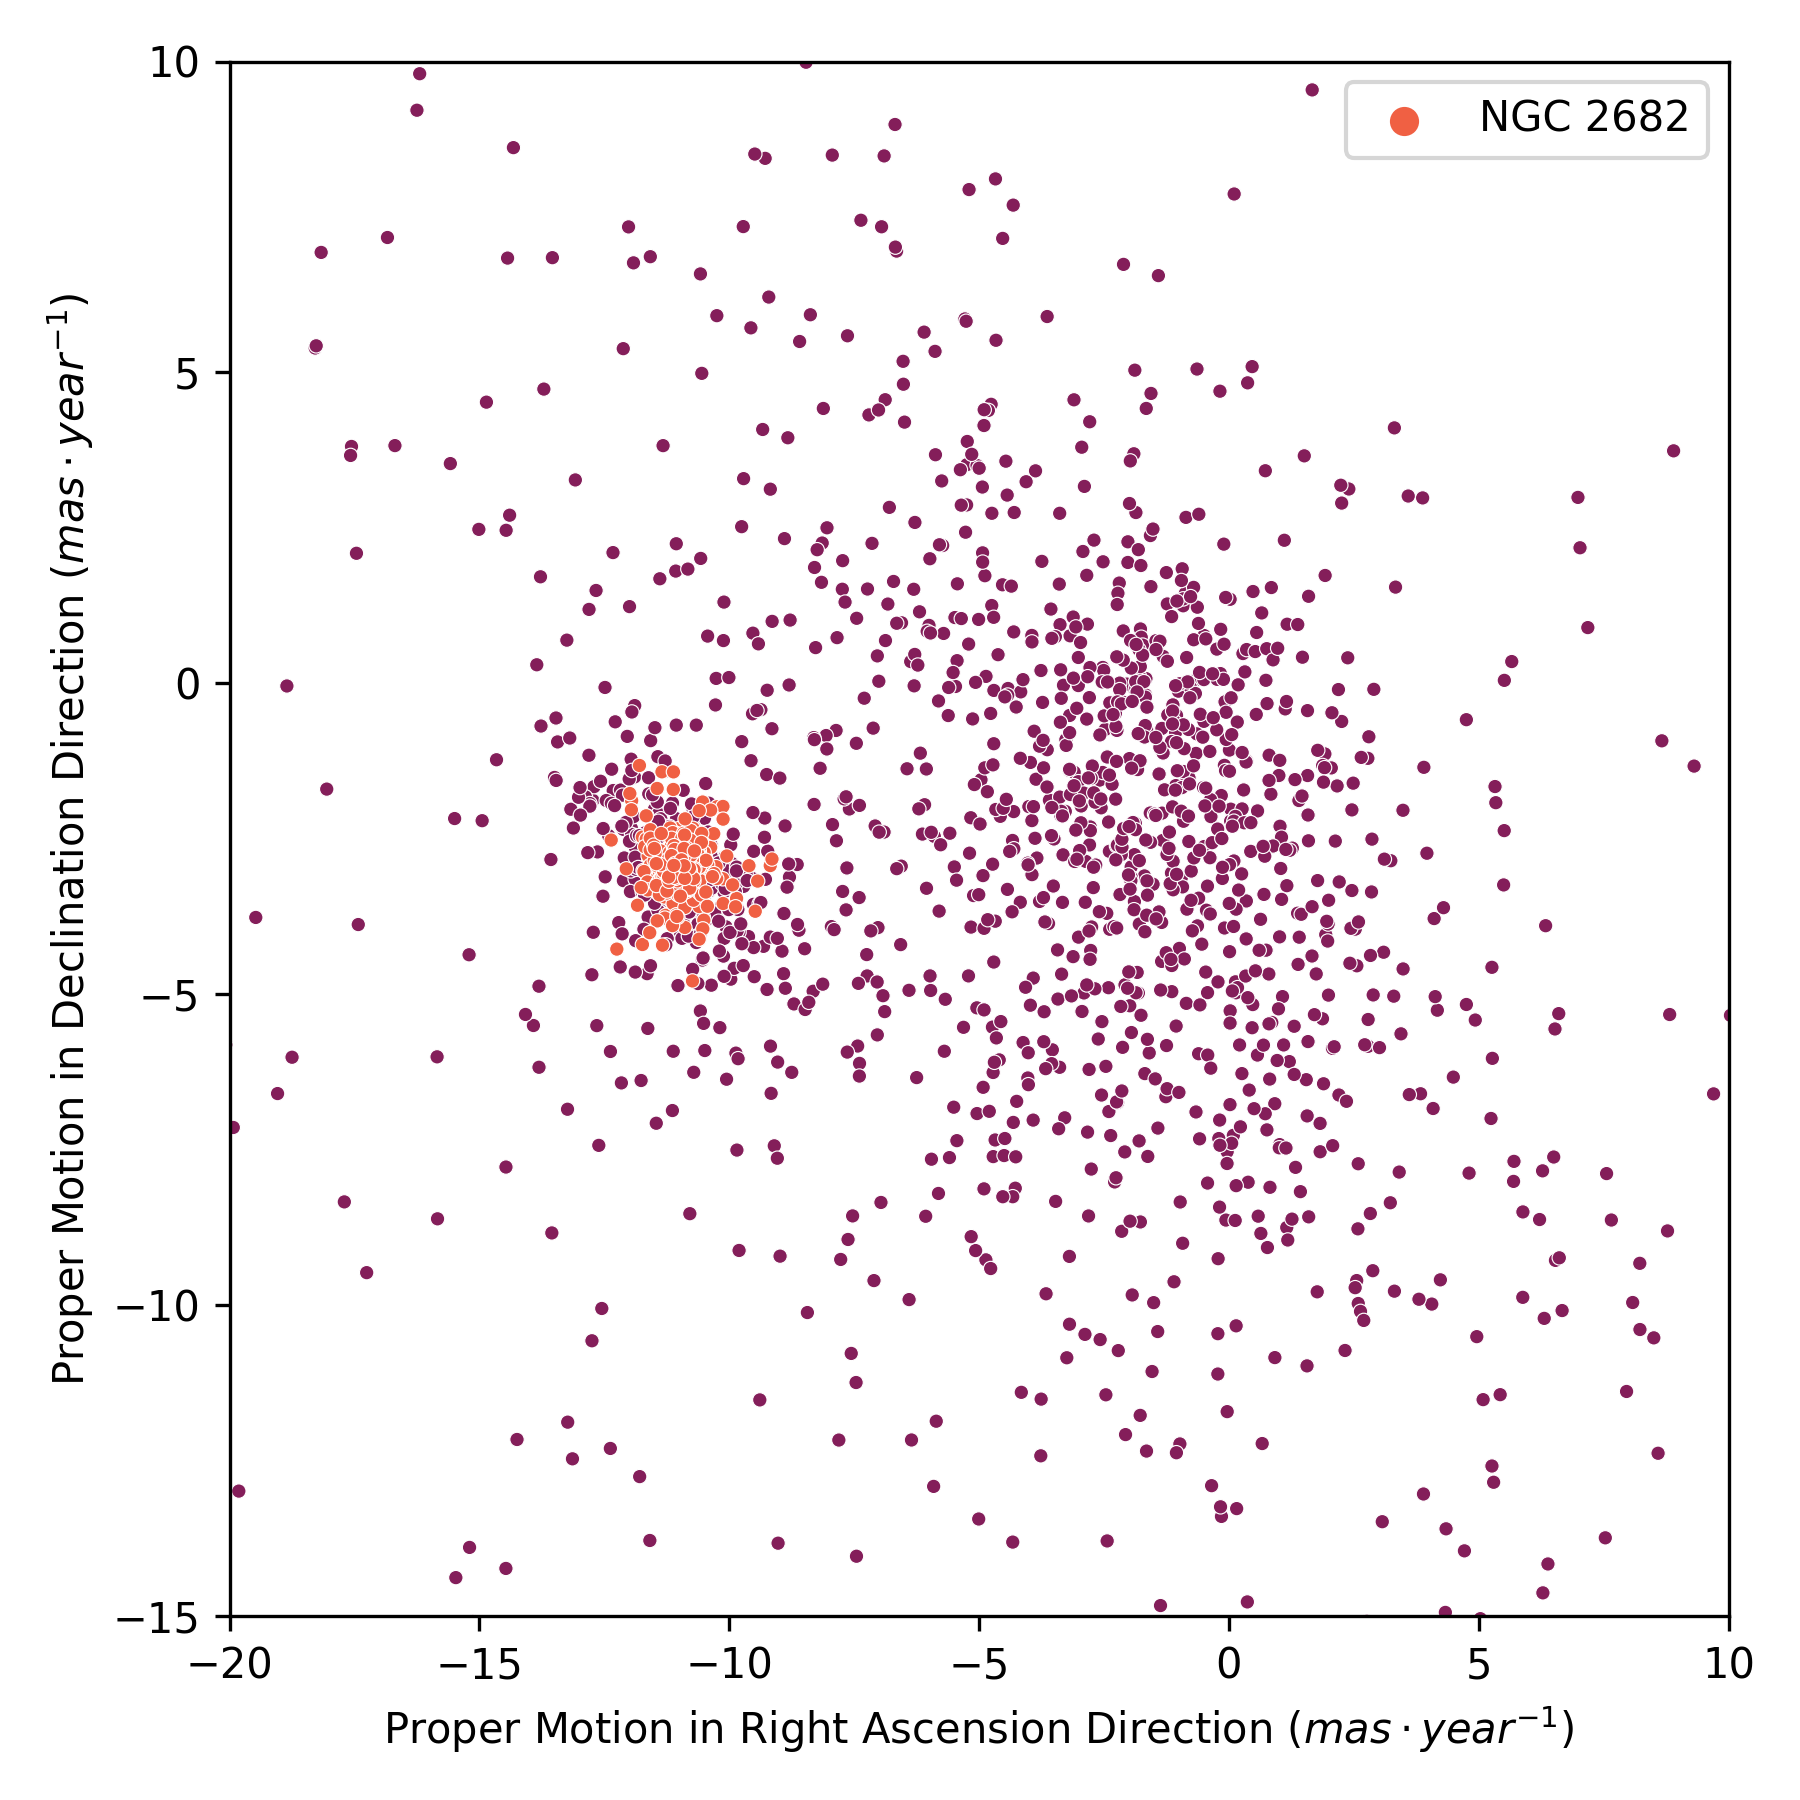
\includegraphics[width=\textwidth]{../figures/ngc_2682/pm_ngc_2682.png}
    \end{subfigure}
    \hfill
    \begin{subfigure}[t]{0.30\textwidth}
      \centering
      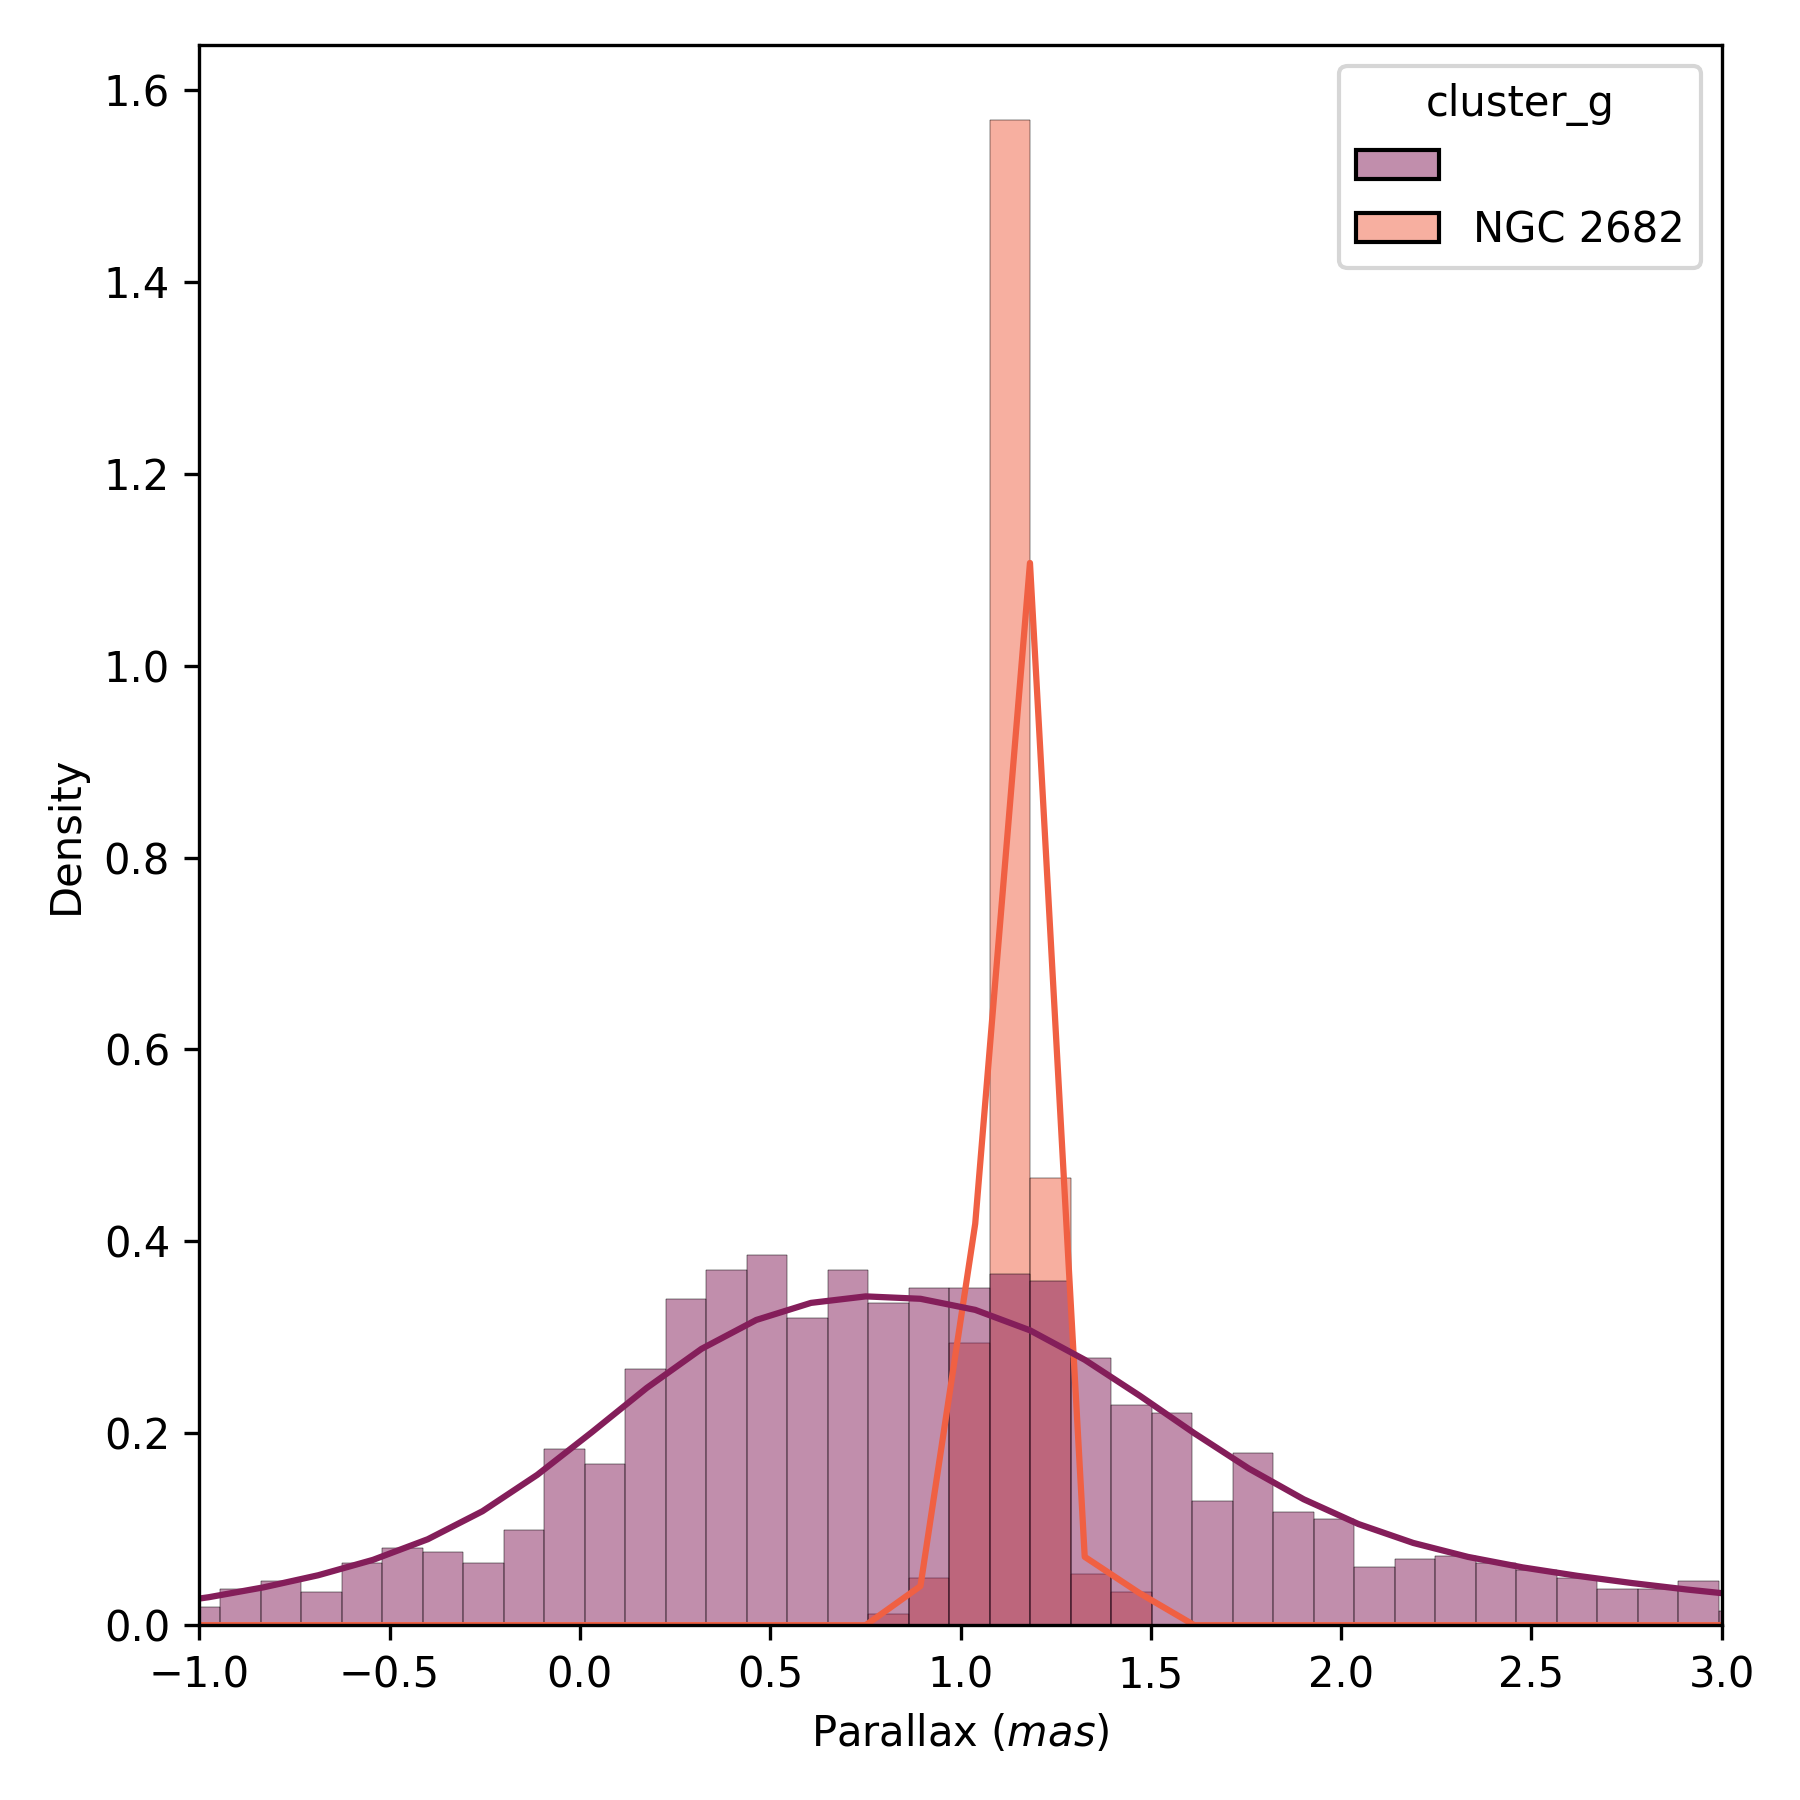
\includegraphics[width=\textwidth]{../figures/ngc_2682/parallax_ngc_2682.png}
    \end{subfigure}
    \hfill
    \begin{subfigure}[t]{0.30\textwidth}
      \centering
      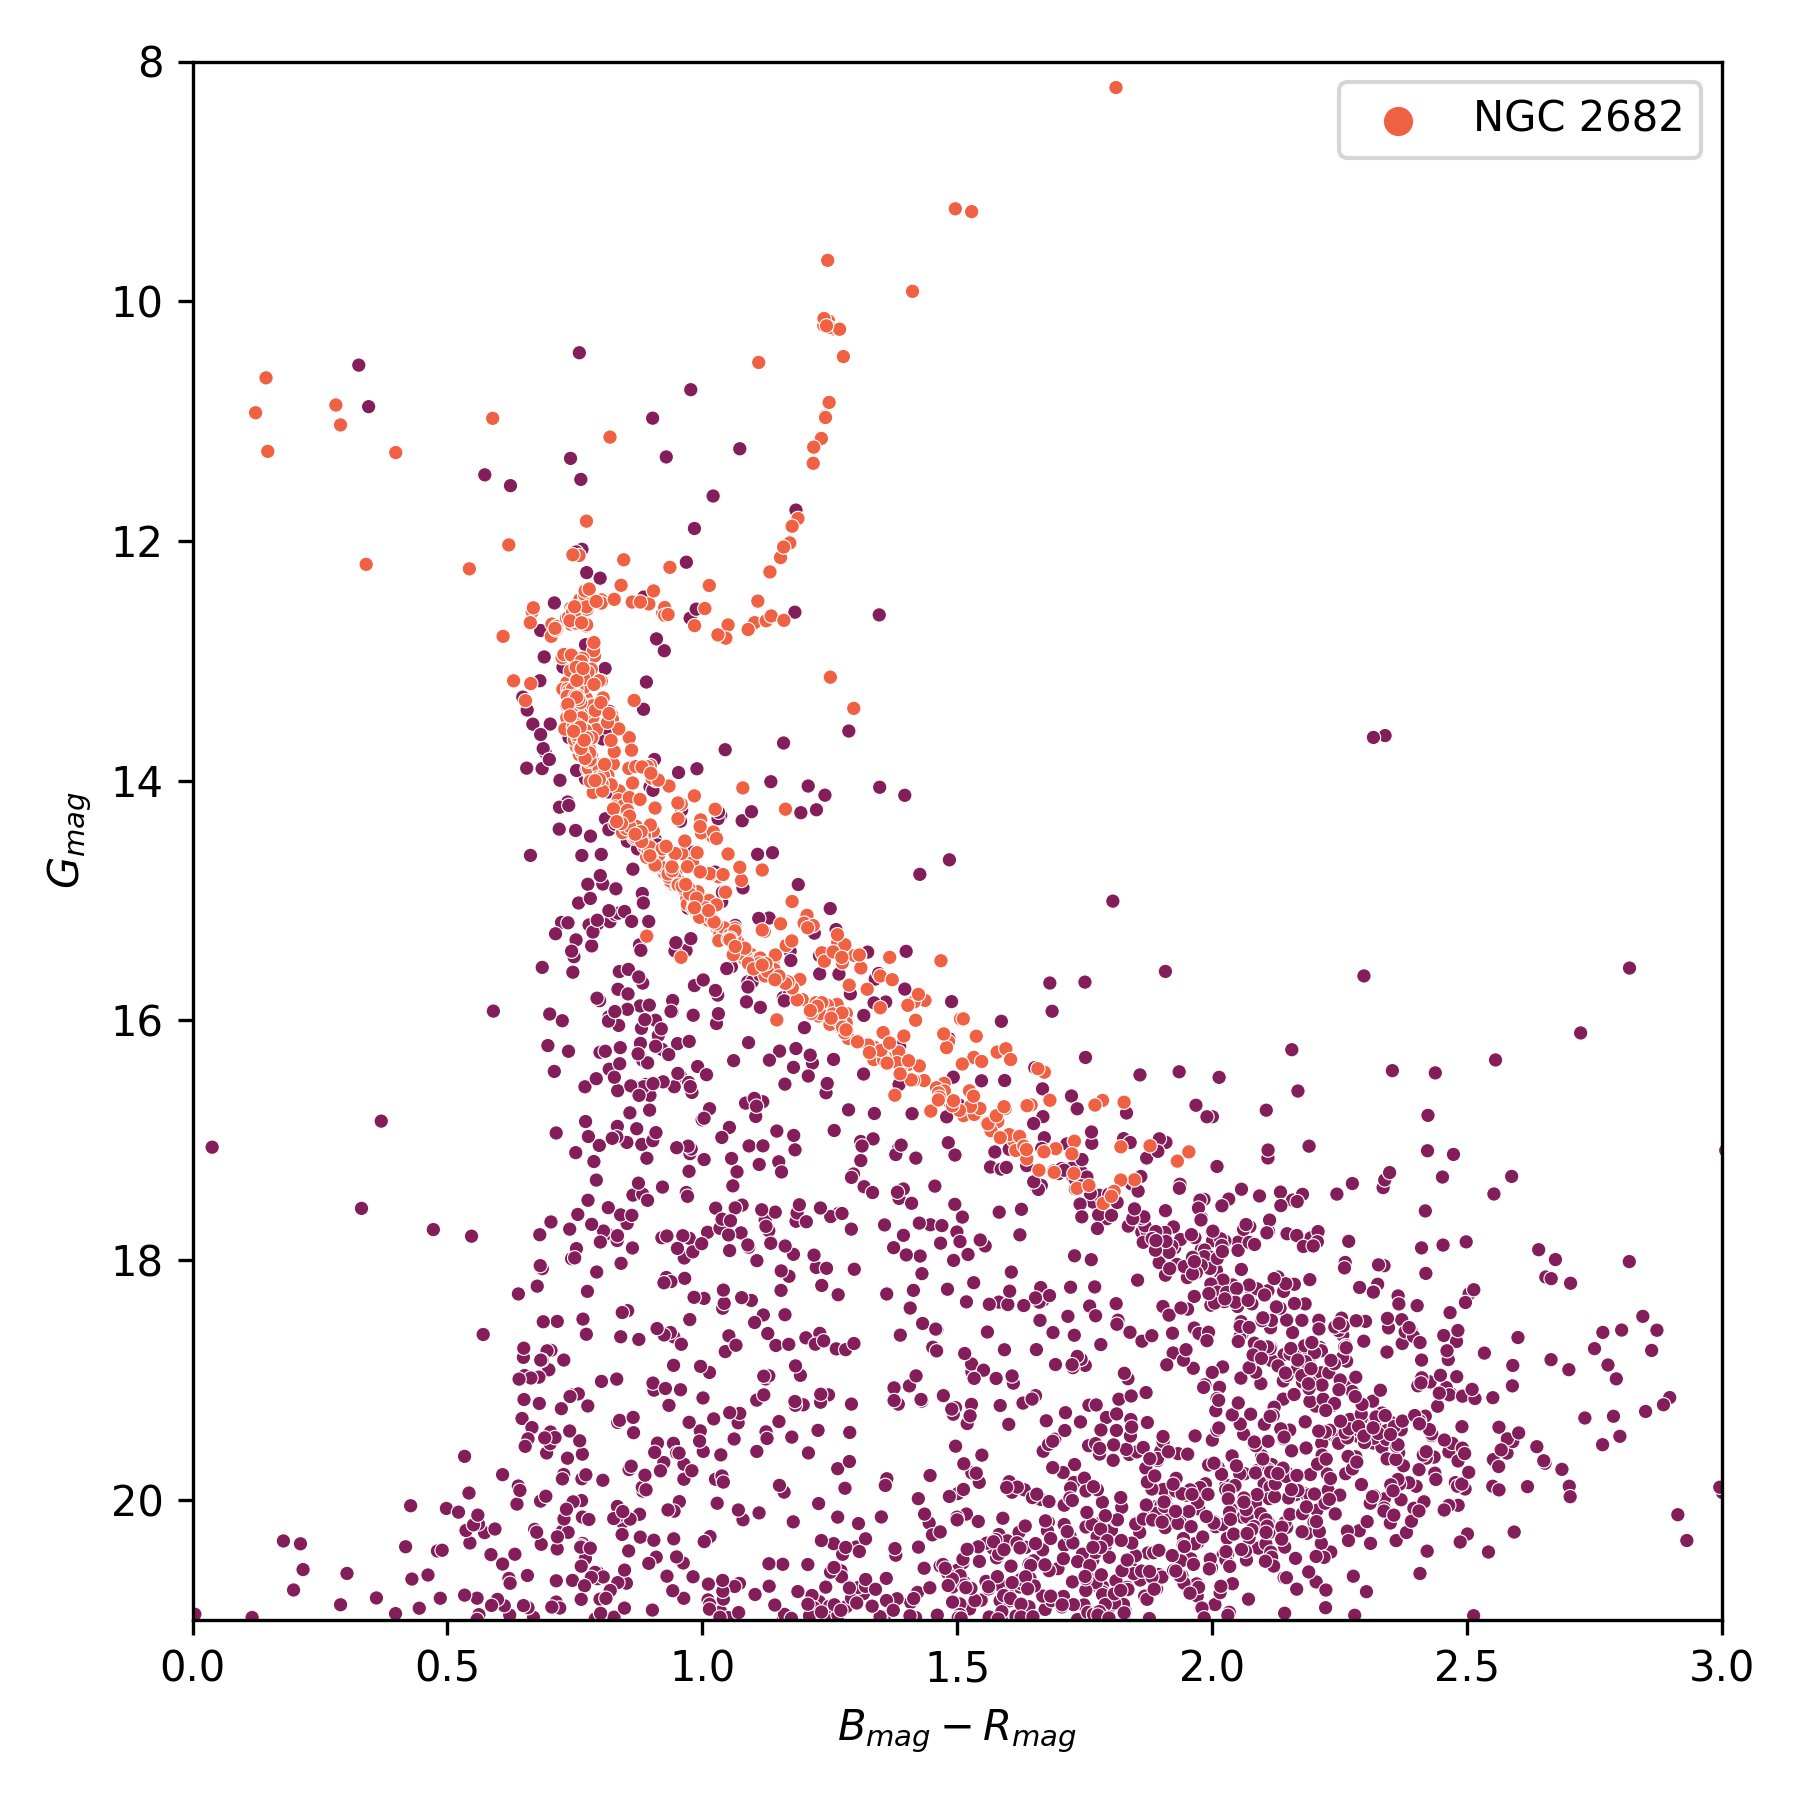
\includegraphics[width=\textwidth]{../figures/ngc_2682/hr_diagram_ngc_2682.png}
    \end{subfigure}
  \end{subfigure}
  \centering
  \begin{subfigure}{\columnwidth}
    \centering
    \begin{subfigure}[t]{0.30\textwidth}
      \centering
      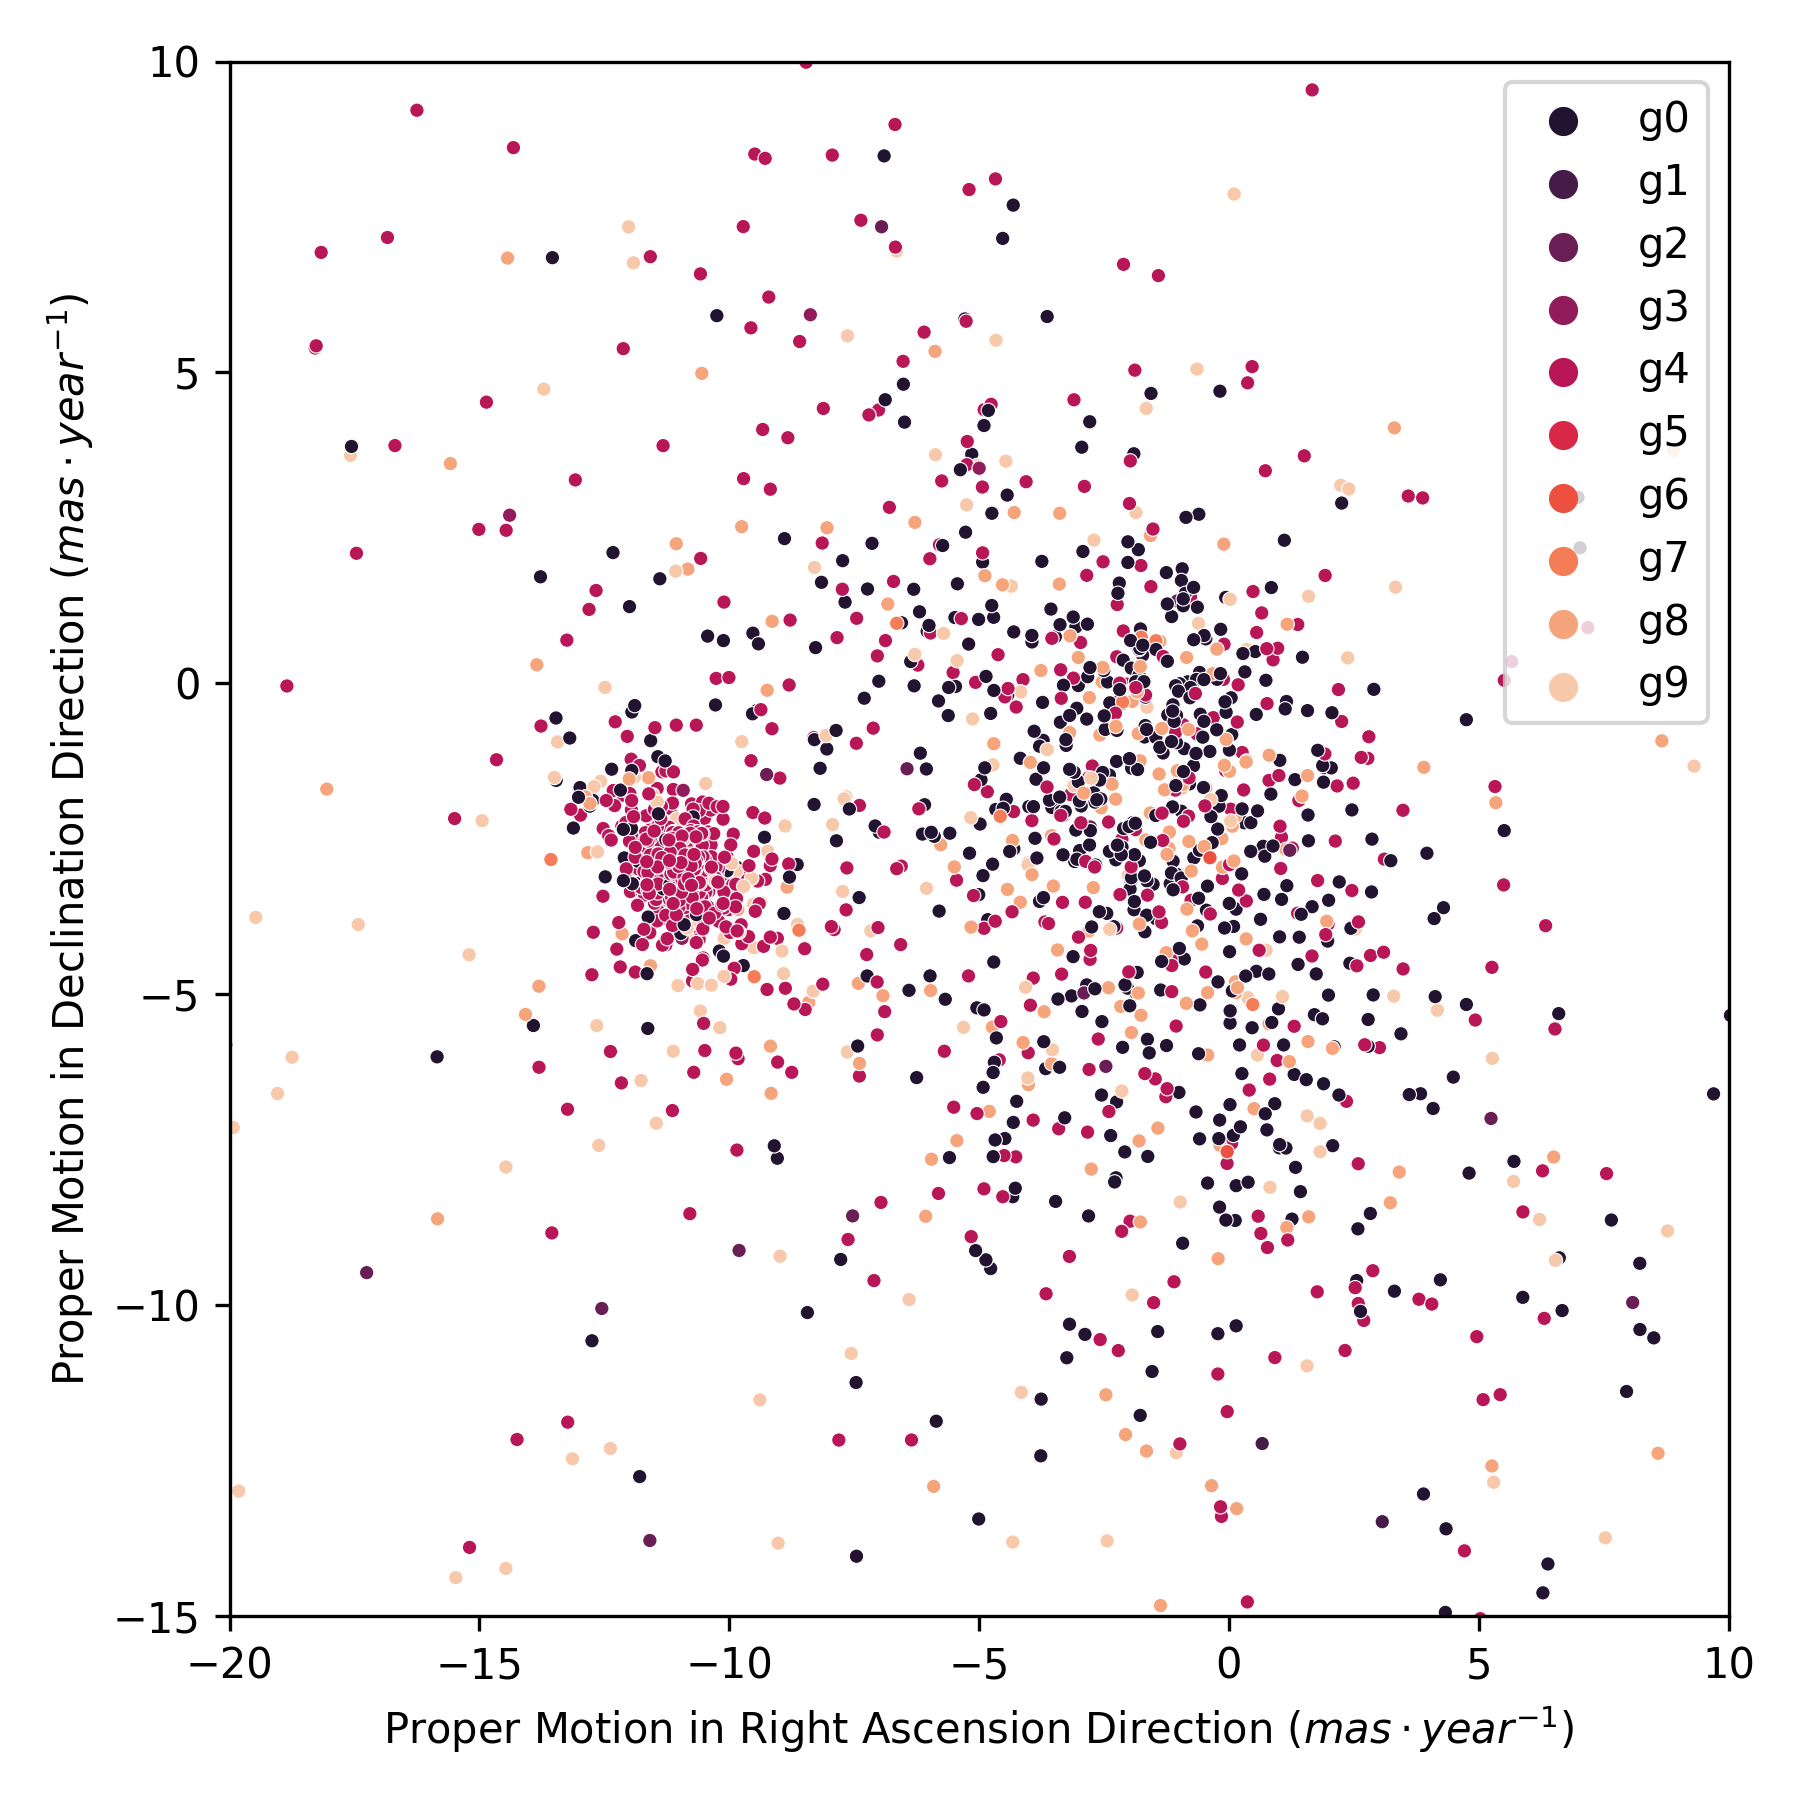
\includegraphics[width=\textwidth]{../figures/ngc_2682/kmeans_pm_ngc_2682.png}
    \end{subfigure}
    \hfill
    \begin{subfigure}[t]{0.30\textwidth}
      \centering
      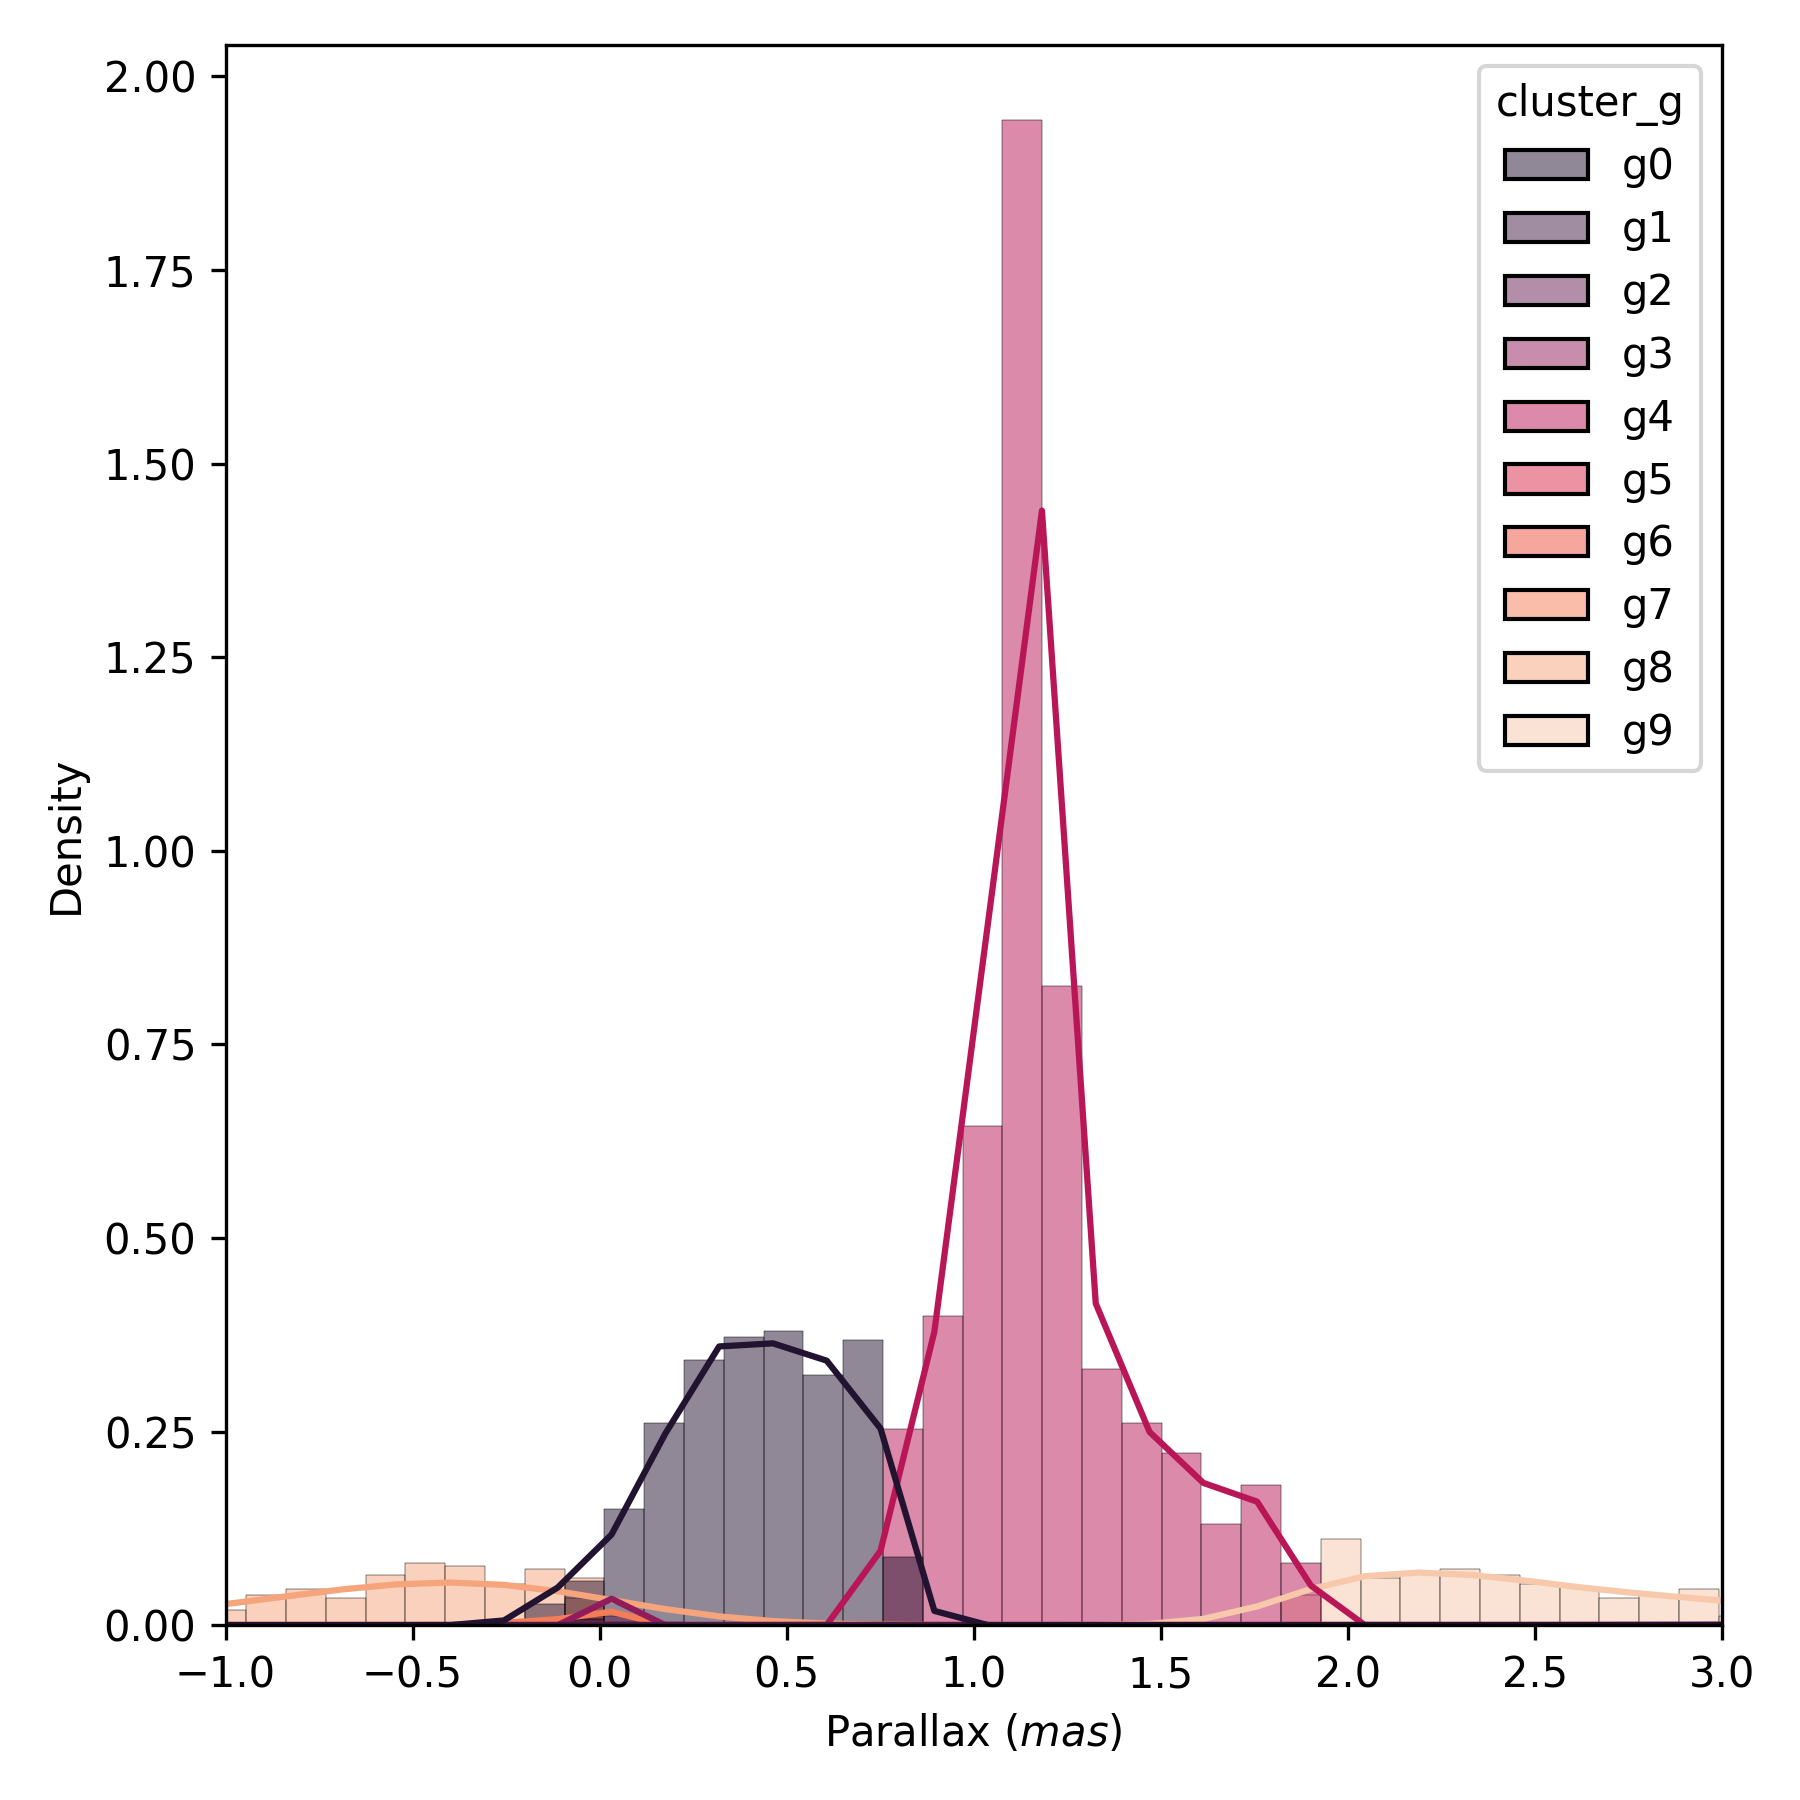
\includegraphics[width=\textwidth]{../figures/ngc_2682/kmeans_parallax_ngc_2682.png}
    \end{subfigure}
    \hfill
    \begin{subfigure}[t]{0.30\textwidth}
      \centering
      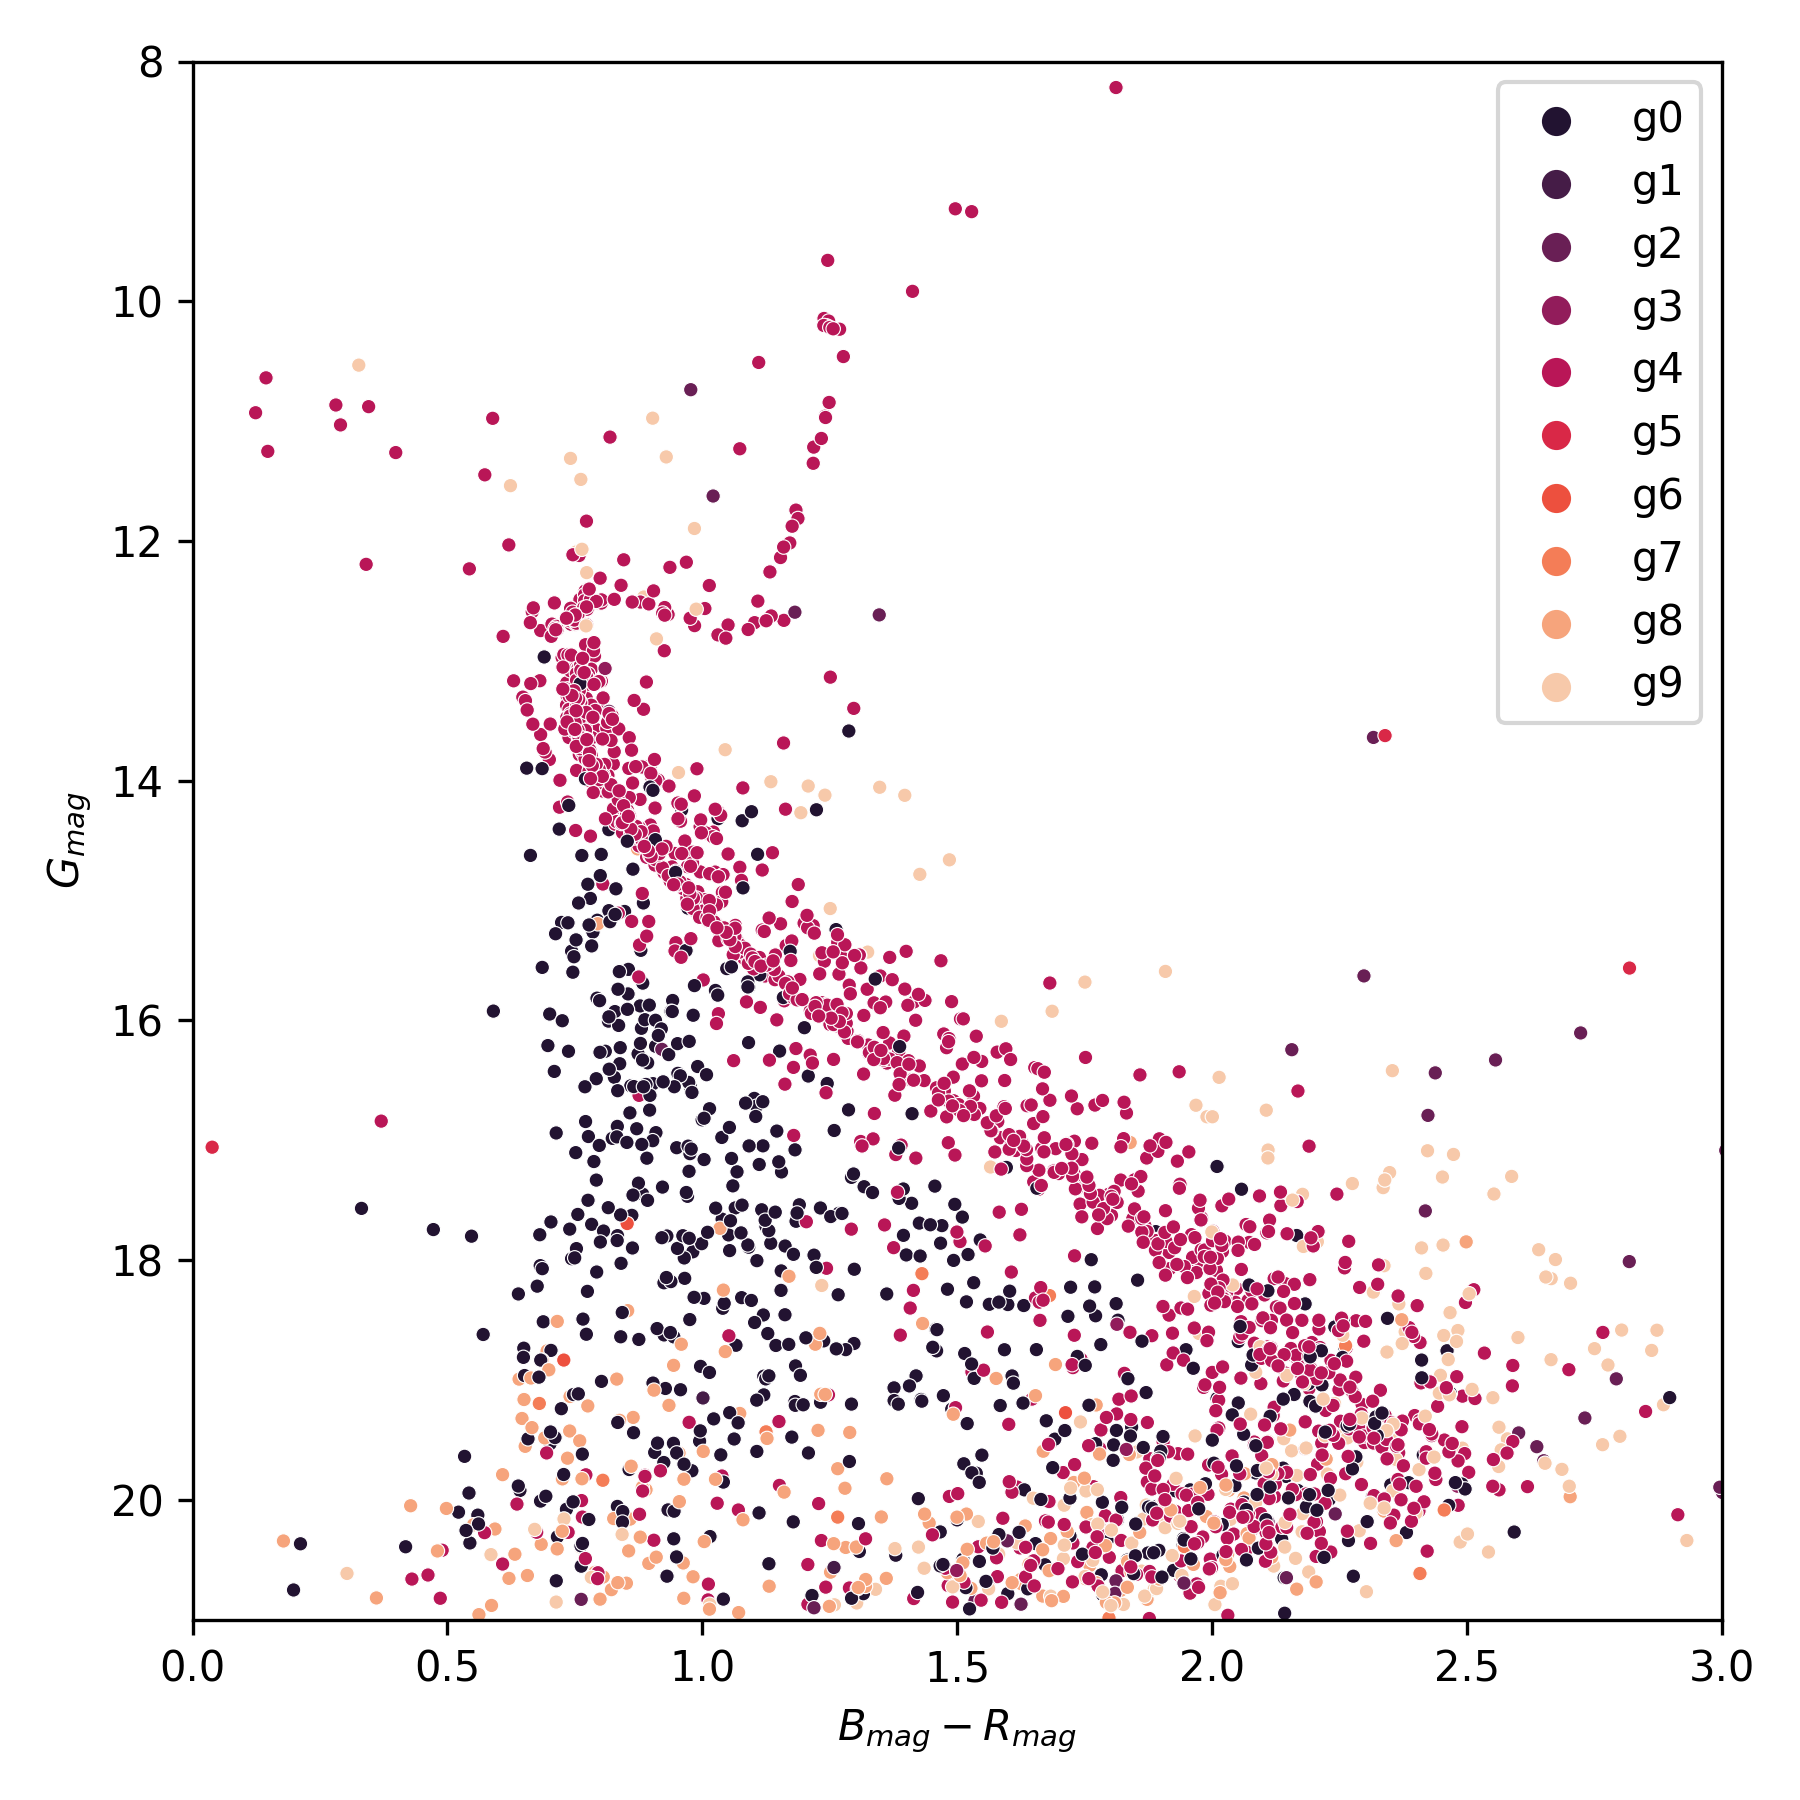
\includegraphics[width=\textwidth]{../figures/ngc_2682/kmeans_hr_diagram_ngc_2682.png}
    \end{subfigure}
  \end{subfigure}
  \caption{NGC 2682 K-Means characterization.
           Top row corresponds to Clusterix+TOPCAT characterization,
           while bottom row shows K-Means results identifying
           NGC 2682 as cluster \emph{g4}.}
  \label{fig:app_result_ngc_2682_clusterix_kmeans}
\end{figure}

Figure~\ref{fig:app_result_ngc_2682_dec} shows the groups found using
the DEC model (first row) and the DEC model filtered (second row).
The cluster of interest is the group \emph{g2}.

\begin{figure}[htbp]
  \centering
  \begin{subfigure}{\columnwidth}
    \centering
    \begin{subfigure}[t]{0.30\textwidth}
      \centering
      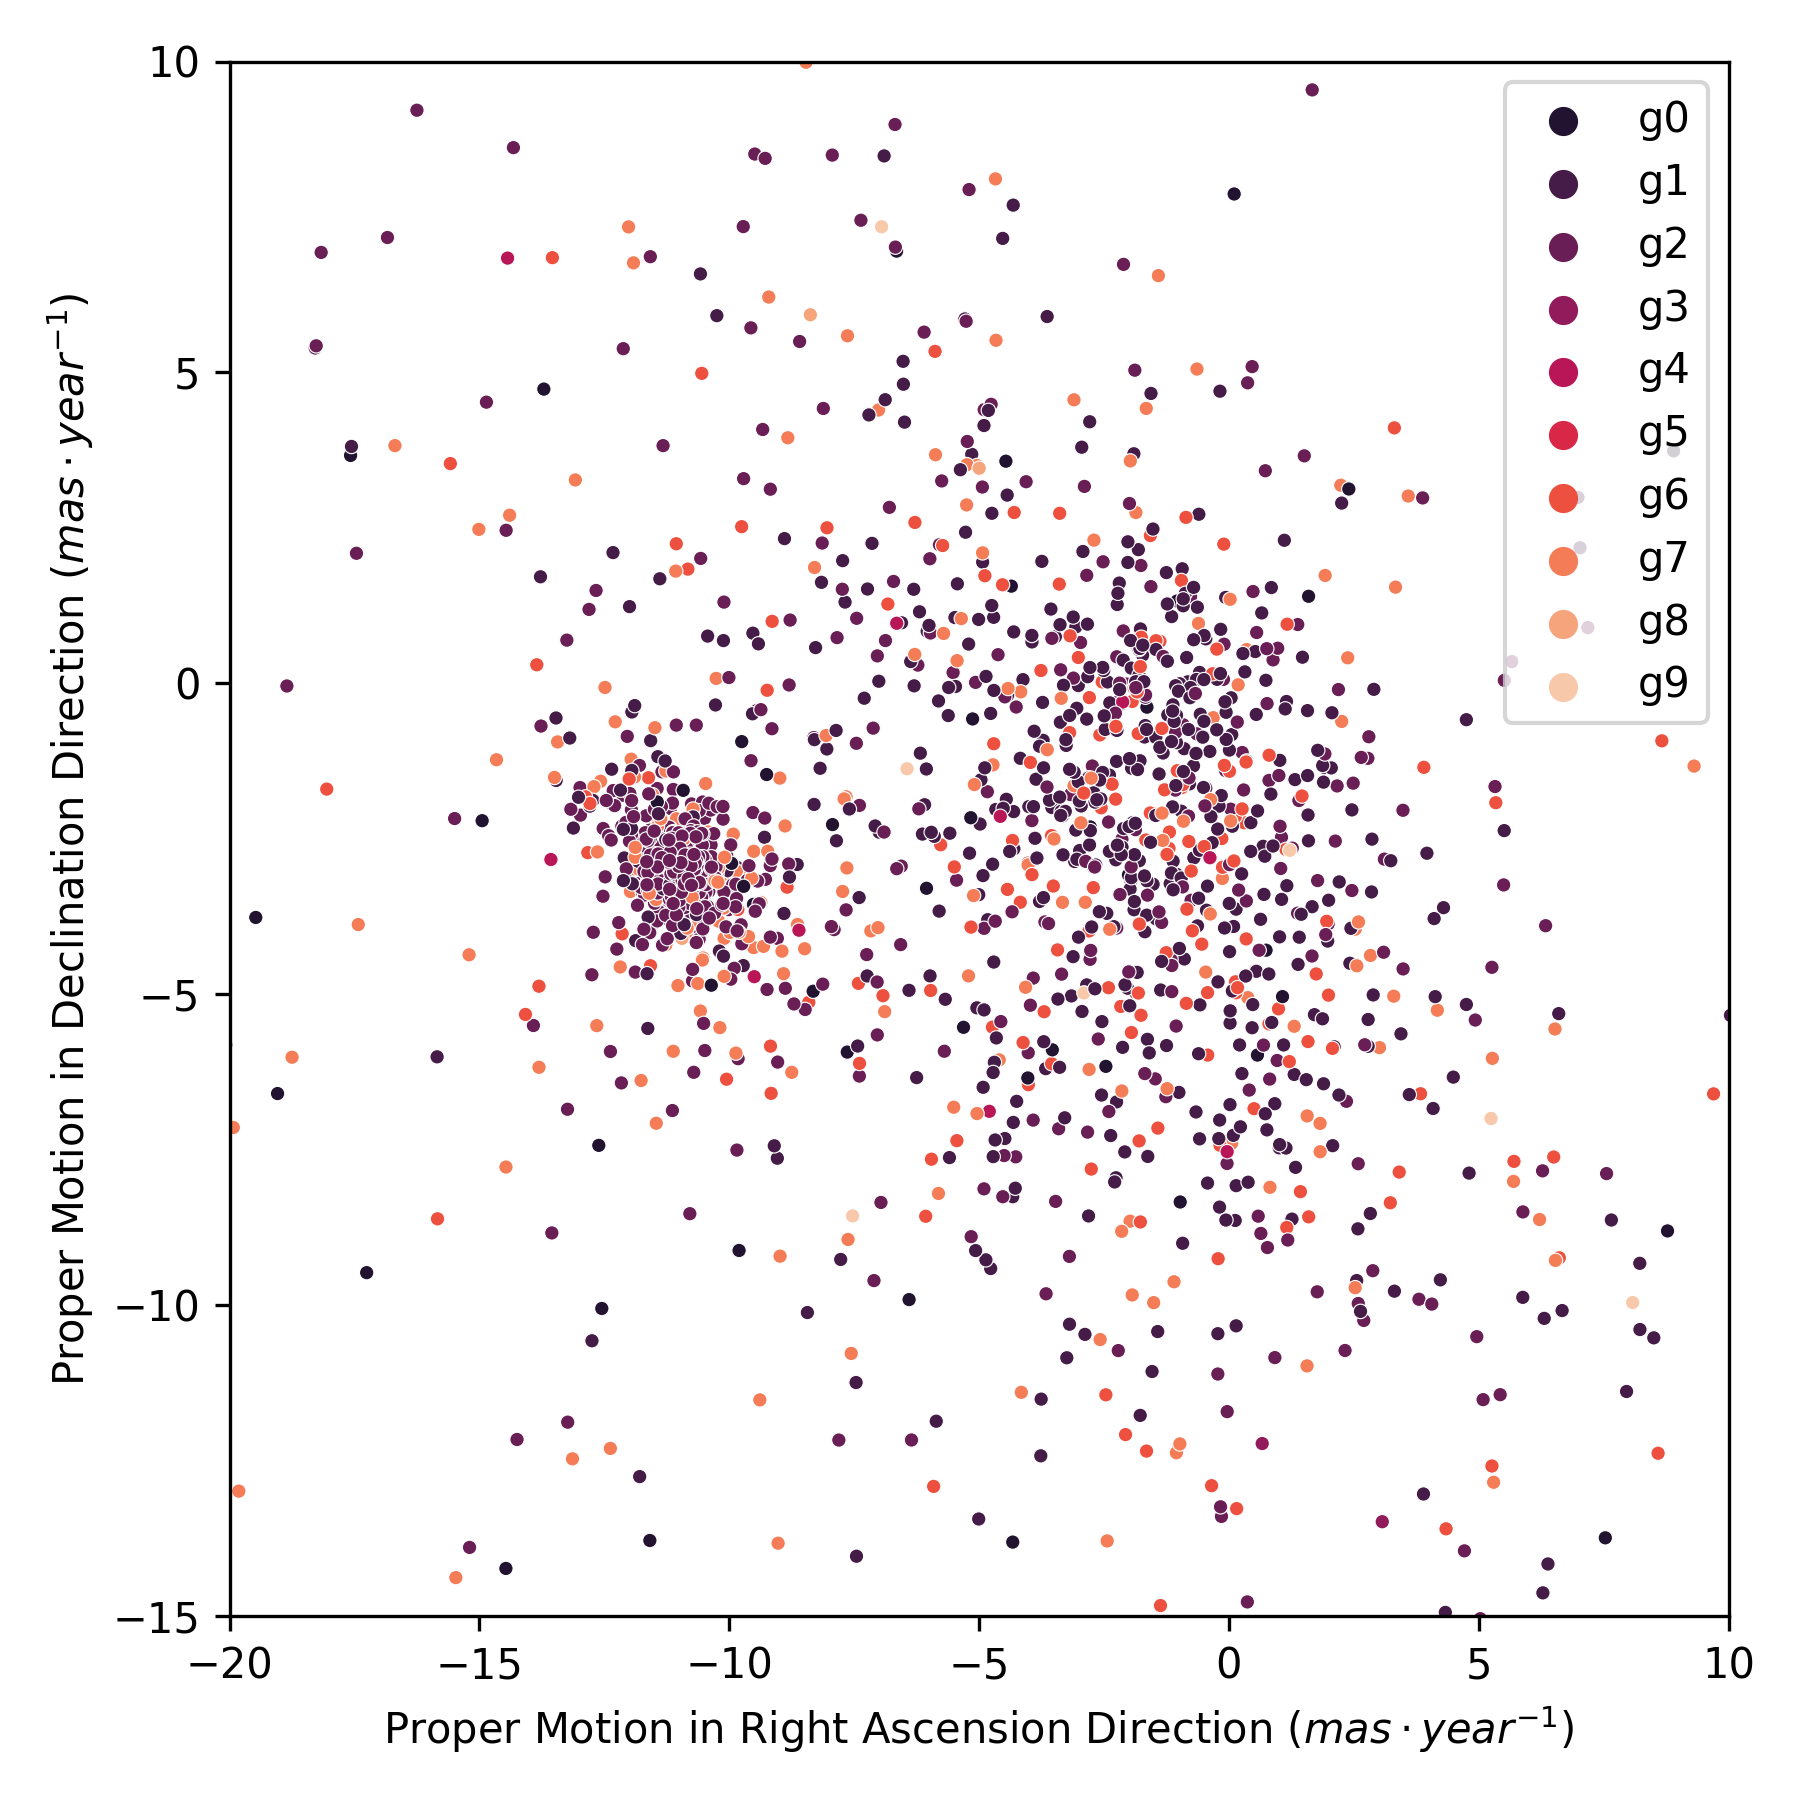
\includegraphics[width=\textwidth]{../figures/ngc_2682/dec_pm_ngc_2682.png}
    \end{subfigure}
    \hfill
    \begin{subfigure}[t]{0.30\textwidth}
      \centering
      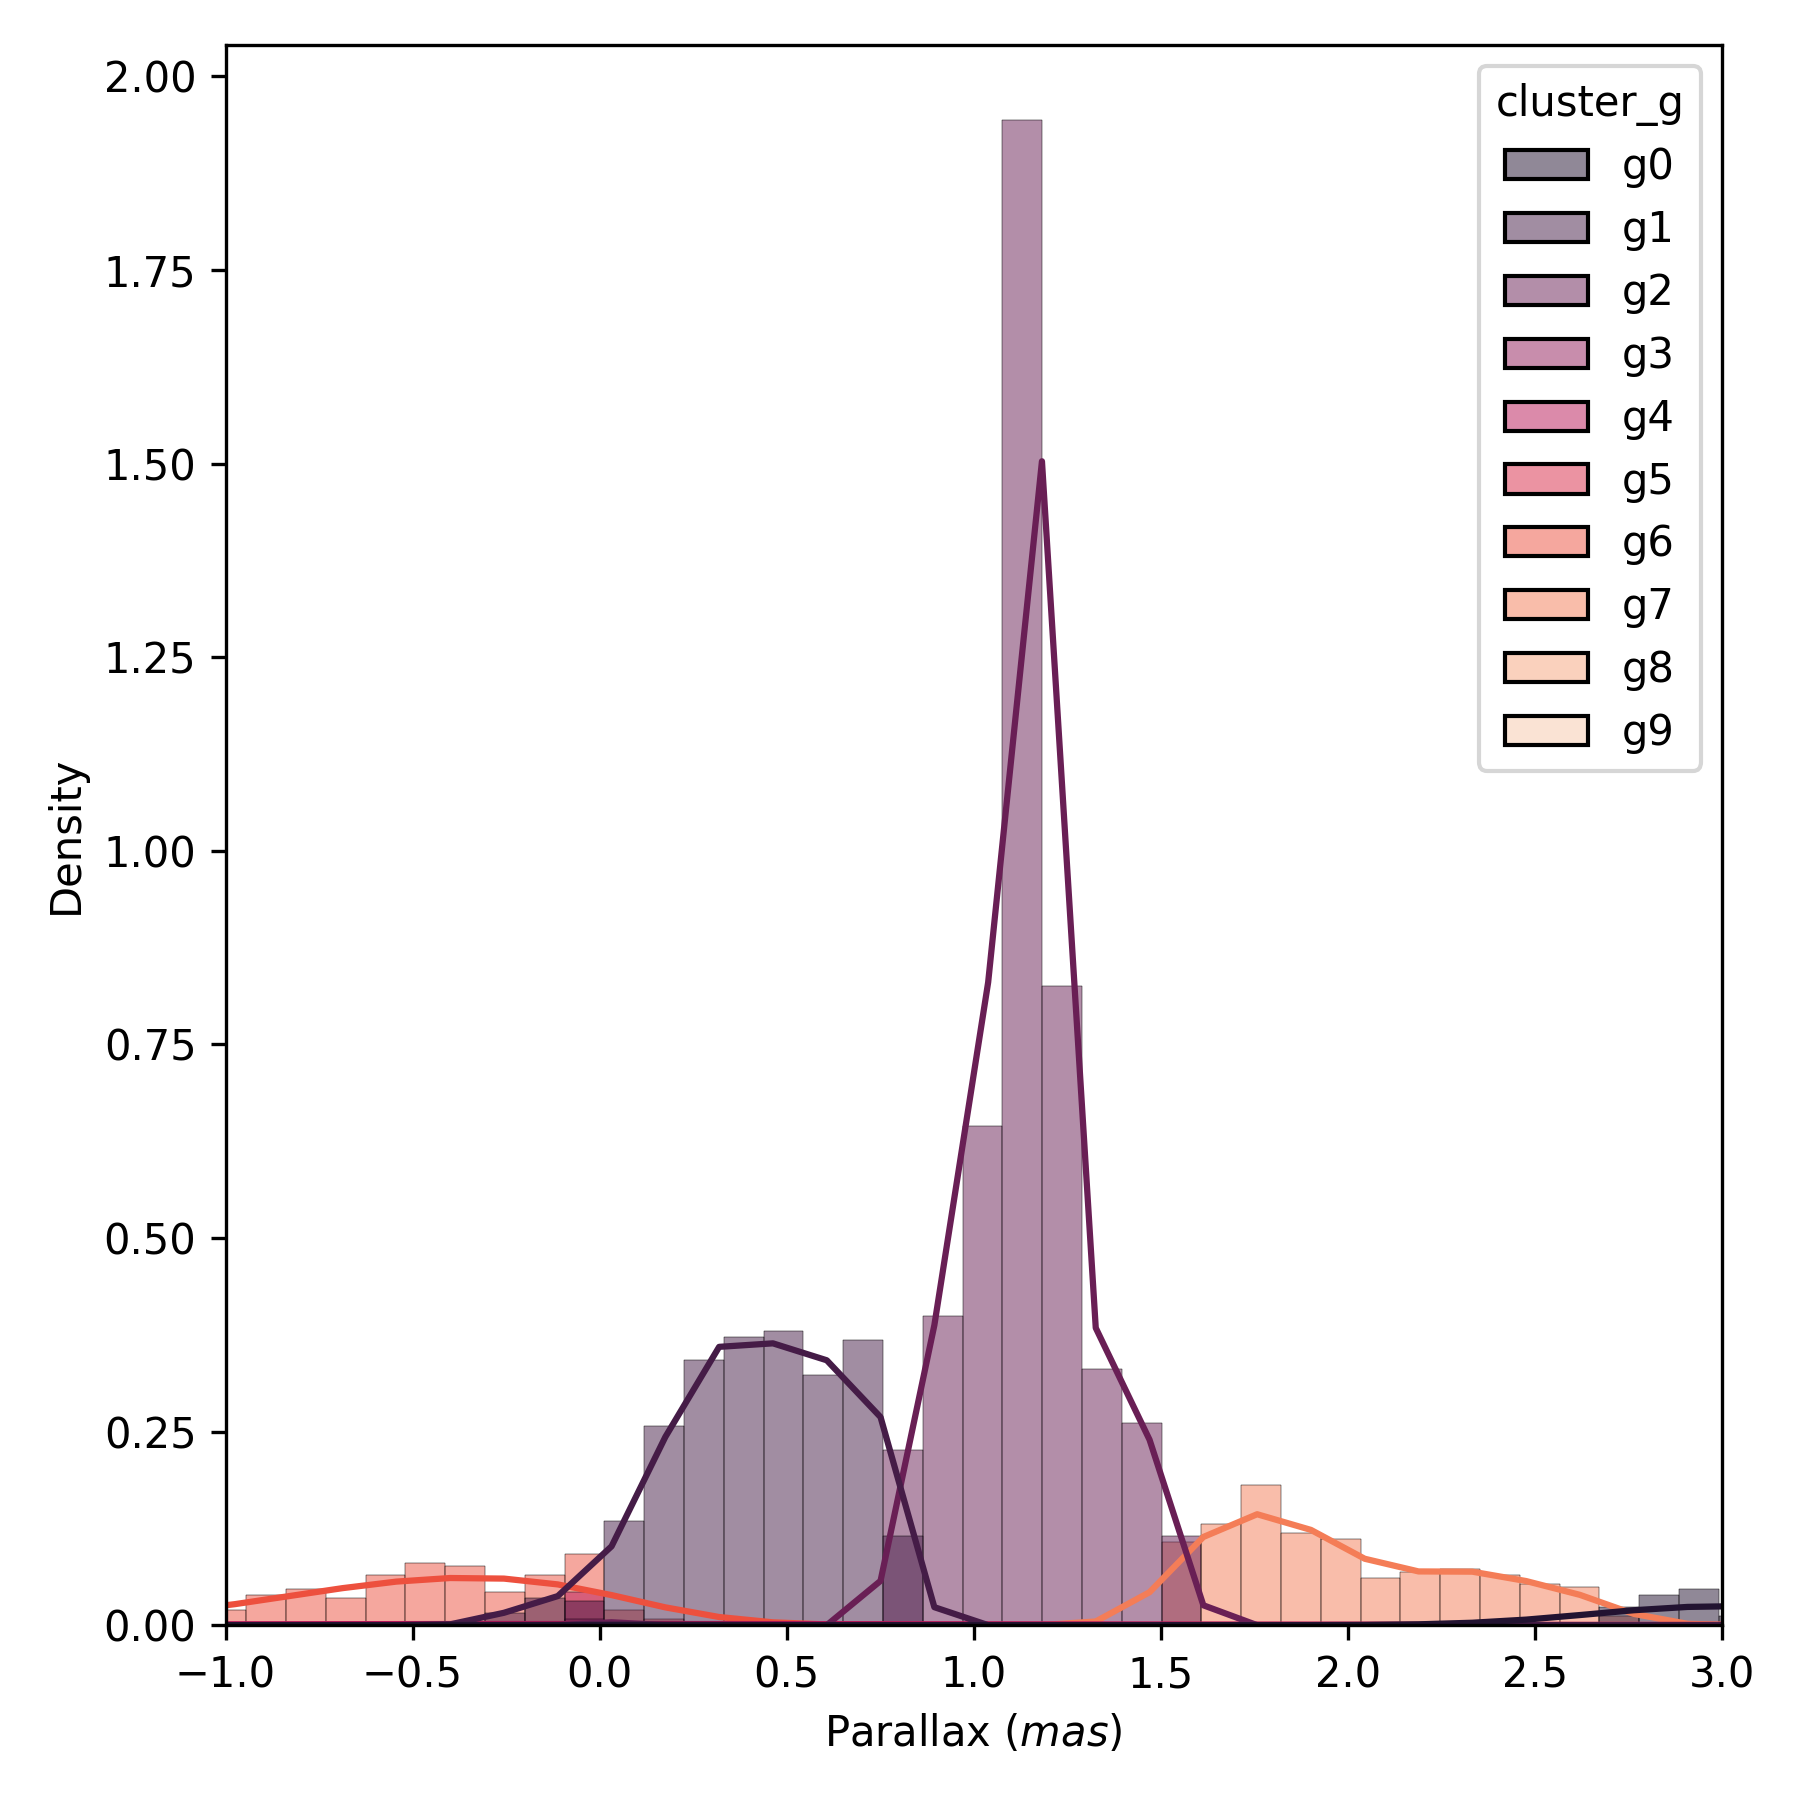
\includegraphics[width=\textwidth]{../figures/ngc_2682/dec_parallax_ngc_2682.png}
    \end{subfigure}
    \hfill
    \begin{subfigure}[t]{0.30\textwidth}
      \centering
      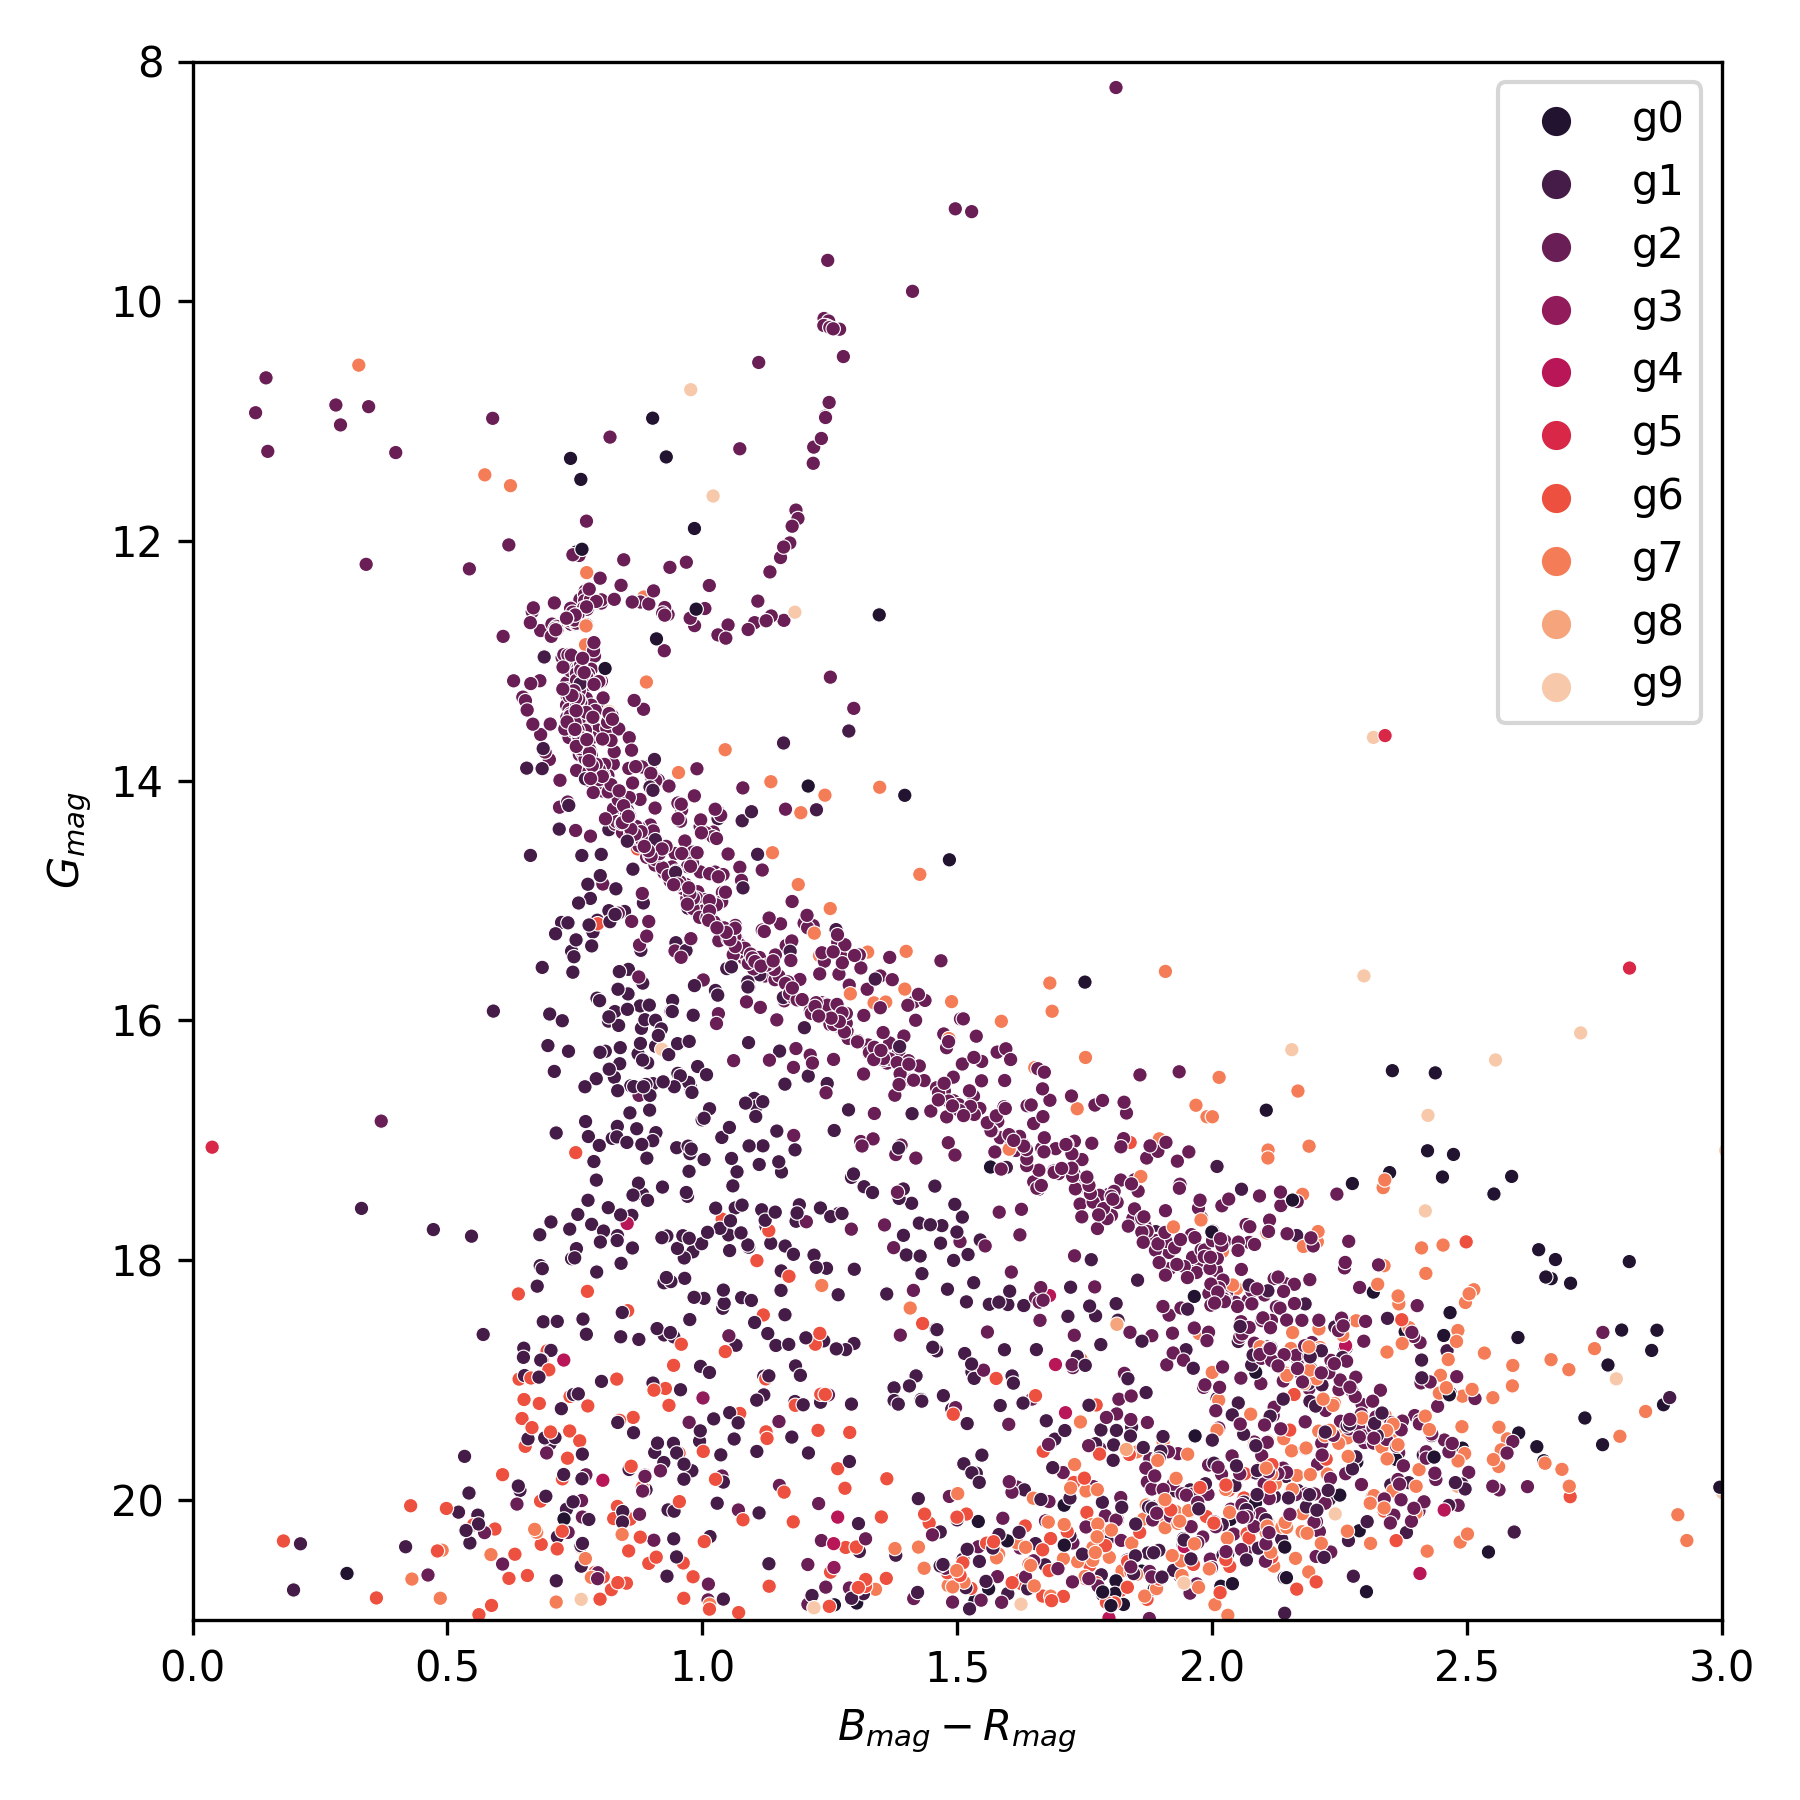
\includegraphics[width=\textwidth]{../figures/ngc_2682/dec_hr_diagram_ngc_2682.png}
    \end{subfigure}
  \end{subfigure}
  \centering
  \begin{subfigure}{\columnwidth}
    \centering
    \begin{subfigure}[t]{0.30\textwidth}
      \centering
      \includegraphics[width=\textwidth]{../figures/ngc_2682/dec_pm_filtered_ngc_2682.png}
    \end{subfigure}
    \hfill
    \begin{subfigure}[t]{0.30\textwidth}
      \centering
      \includegraphics[width=\textwidth]{../figures/ngc_2682/dec_parallax_filtered_ngc_2682.png}
    \end{subfigure}
    \hfill
    \begin{subfigure}[t]{0.30\textwidth}
      \centering
      \includegraphics[width=\textwidth]{../figures/ngc_2682/dec_hr_diagram_filtered_ngc_2682.png}
    \end{subfigure}
  \end{subfigure}
  \caption{NGC 2682 is identified as cluster \emph{g2}.
           Top row: DEC --- Bottom row: DEC (filtered)}
  \label{fig:app_result_ngc_2682_dec}
\end{figure}

Table~\ref{tab:app_hyperparameters_ngc_2682} shows the
hyperparameters used for characterizing NGC 2682 with DEC method.

\begin{table}[htbp]
  \begin{center}
    \begin{tabular}{l|c}
      \textbf{Hyperparameter} & \textbf{Value} \\
      \hline
      Number of Clusters & 10 \\
      Clustering Layer & \(\left[ 50, 50, 40 \right]\) \\
      Kernel Initializer Seed & 0 \\
      Quantil Threshold & 0.1 \\
    \end{tabular}
    \caption{NGC 2682 DEC hyperparameters.}
    \label{tab:app_hyperparameters_ngc_2682}
  \end{center}
\end{table}

\subsection{Melotte 22}
\label{sec:melotte22}

\begin{figure}[htbp]
  \centering
  \begin{subfigure}{\columnwidth}
    \centering
    \begin{subfigure}[t]{0.30\textwidth}
      \centering
      \includegraphics[width=\textwidth]{../figures/melotte_22/pm_melotte_22.png}
    \end{subfigure}
    \hfill
    \begin{subfigure}[t]{0.30\textwidth}
      \centering
      \includegraphics[width=\textwidth]{../figures/melotte_22/parallax_melotte_22.png}
    \end{subfigure}
    \hfill
    \begin{subfigure}[t]{0.30\textwidth}
      \centering
      \includegraphics[width=\textwidth]{../figures/melotte_22/hr_diagram_melotte_22.png}
    \end{subfigure}
  \end{subfigure}
  \centering
  \begin{subfigure}{\columnwidth}
    \centering
    \begin{subfigure}[t]{0.30\textwidth}
      \centering
      \includegraphics[width=\textwidth]{../figures/melotte_22/kmeans_pm_melotte_22.png}
    \end{subfigure}
    \hfill
    \begin{subfigure}[t]{0.30\textwidth}
      \centering
      \includegraphics[width=\textwidth]{../figures/melotte_22/kmeans_parallax_melotte_22.png}
    \end{subfigure}
    \hfill
    \begin{subfigure}[t]{0.30\textwidth}
      \centering
      \includegraphics[width=\textwidth]{../figures/melotte_22/kmeans_hr_diagram_melotte_22.png}
    \end{subfigure}
  \end{subfigure}
  \caption{Melotte 22 characterization.
           Top row: Clusterix+TOPCAT. Bottom row: K-Means.
           Melotte 22 is labeled as cluster \emph{g1}.}
  \label{fig:app_result_melotte_22_clusterix_kmeans}
\end{figure}

Figure~\ref{fig:app_result_melotte_22_clusterix_kmeans} shows Melotte 22
characterized using Clusterix+TOPCAT tools (top row) and the characterization
made by K-Means (bottom row) showing nine clusters. Melotte 22 is labeled as
group \emph{g1}.

Figure~\ref{fig:app_result_melotte_22_dec} shows the groups found using
DEC model (first row) and DEC model filtered (second row).
Melotte 22 is labeled as group \emph{g2} by DEC model.

\begin{figure}[htbp]
  \centering
  \begin{subfigure}{\columnwidth}
    \centering
    \begin{subfigure}[t]{0.30\textwidth}
      \centering
      \includegraphics[width=\textwidth]{../figures/melotte_22/dec_pm_melotte_22.png}
    \end{subfigure}
    \hfill
    \begin{subfigure}[t]{0.30\textwidth}
      \centering
      \includegraphics[width=\textwidth]{../figures/melotte_22/dec_parallax_melotte_22.png}
    \end{subfigure}
    \hfill
    \begin{subfigure}[t]{0.30\textwidth}
      \centering
      \includegraphics[width=\textwidth]{../figures/melotte_22/dec_hr_diagram_melotte_22.png}
    \end{subfigure}
  \end{subfigure}
  \centering
  \begin{subfigure}{\columnwidth}
    \centering
    \begin{subfigure}[t]{0.30\textwidth}
      \centering
      \includegraphics[width=\textwidth]{../figures/melotte_22/dec_pm_filtered_melotte_22.png}
    \end{subfigure}
    \hfill
    \begin{subfigure}[t]{0.30\textwidth}
      \centering
      \includegraphics[width=\textwidth]{../figures/melotte_22/dec_parallax_filtered_melotte_22.png}
    \end{subfigure}
    \hfill
    \begin{subfigure}[t]{0.30\textwidth}
      \centering
      \includegraphics[width=\textwidth]{../figures/melotte_22/dec_hr_diagram_filtered_melotte_22.png}
    \end{subfigure}
  \end{subfigure}
  \caption{Melotte 22 is identified as cluster \emph{g2}.
           Top row: DEC --- Bottom row: DEC (filtered)}
  \label{fig:app_result_melotte_22_dec}
\end{figure}

Table~\ref{tab:app_results_melotte_22} shows a results summary for Melotte 22.

\begin{table}[htbp]
  \begin{center}
    \resizebox{\columnwidth}{!}{
      \begin{tabular}{l|c|c|c|c}
        \textbf{Method} & \emph{\(\mu_{\alpha}\) \((mas \cdot yr^{-1})\)} & \emph{\(\mu_{\delta}\) \((mas \cdot yr^{-1})\)}
        & \emph{\( \varpi \) \((mas)\)} & \emph{\# stars} \\
        \hline
        \textbf{Simbad} & 19.997 \( \pm \) 0.127 & -45.548 \( \pm \) 0.101 & 7.364 \( \pm \) 0.005 & 1326 \\
        Clusterix & 19.98 \( \pm \) 1.25 & -45.47 \( \pm \) 1.48 & 7.33 \( \pm \) 0.21 & 634 \\
        K-Means & 20.25 \( \pm \) 0.95 & -38.01 \( \pm \) 1.08 & 7.23 \( \pm \) 0.06 & 1378 \\
        DEC & 23.67 \( \pm \) 1.29 & -46.23 \( \pm \) 1.50 & 8.04 \( \pm \) 0.09 & 878 \\
        \textbf{DEC (filt.)} & 19.50 \( \pm \) 0.41 & -44.23 \( \pm \) 0.39 & 7.42 \( \pm \) 0.005 & 438 \\
      \end{tabular}
    }
    \caption{Melotte 22 results.}
    \label{tab:app_results_melotte_22}
  \end{center}
\end{table}

While Table~\ref{tab:app_hyperparameters_melotte_22} shows the hyperparameters
used for characterizing Melotte 22 with the DEC model.

\begin{table}[hbtp]
  \begin{center}
    \begin{tabular}{l|c}
      \textbf{Hyperparameter} & \textbf{Value} \\
      \hline
      Number of Clusters & 5 \\
      Clustering Layer & \(\left[ 50, 50, 200 \right]\) \\
      Kernel Initializer Seed & 11 \\
      Quantil Threshold & 0.1 \\
    \end{tabular}
    \caption{Melotte 22 DEC hyperparameters.}
    \label{tab:app_hyperparameters_melotte_22}
  \end{center}
\end{table}

\renewcommand{\refname}{References}
\bibliographystyle{unsrt}
\bibliography{references}

\end{document}
